% Лабораторная работа по РЗП № 3
% Дуников Константин Артёмович

% Тип документа: статья, на бумаге А4
\documentclass[a4paper]{article}

% Подключение сторонних tex файлов 
\usepackage{import}


% Основные данные - ВУЗ, факультет, город...
\import{./../../../stuff/tex}{config.tex}

% Подключение необходимых зависимостей
\import{./../../../stuff/tex/settings}{packages.tex}
% Настройка подключенных пакетов
\import{./../../../stuff/tex/settings}{preferences.tex}


% Шаблон титульной страницы 
\import{./../../../stuff/tex/templates}{title.tex}
% Упрощенный блок "выполнил"
\import{./../../../stuff/tex/templates}{sign1.tex}
% Макрос для содержания
\import{./../../../stuff/tex/templates}{toc.tex}

% Определяем название документа
\title{
  Лабораторная работа №1 по курсу \\
  <<Разработка защищенных приложений>> \\
  Атака XSS
}
% Отключаем отображение правительства
\renewcommand{\government}{}
% Отключаем сокращенное нзавание университета
\renewcommand{\subuniversity}{}
% Указываем преподавателя
\renewcommand{\shortteachername}{Башун В.В.}


% Путь до внешних изображений
\graphicspath{ {./../figures/xss}}


% Основной текст работы
\begin{document}
  \templatedtitlepage
  
  \toc
  \section{Ход работы}

  \subsection{Запуск ВМ и проверка эндпоинта для захвата параметров}

  Настраиваем и запускаем виртуальную машину, используя для этого зара-нее подготовленный образ,
  в котором уже установлено всё необходимое ПО:

  \begin{figure}[H]
    \centering
    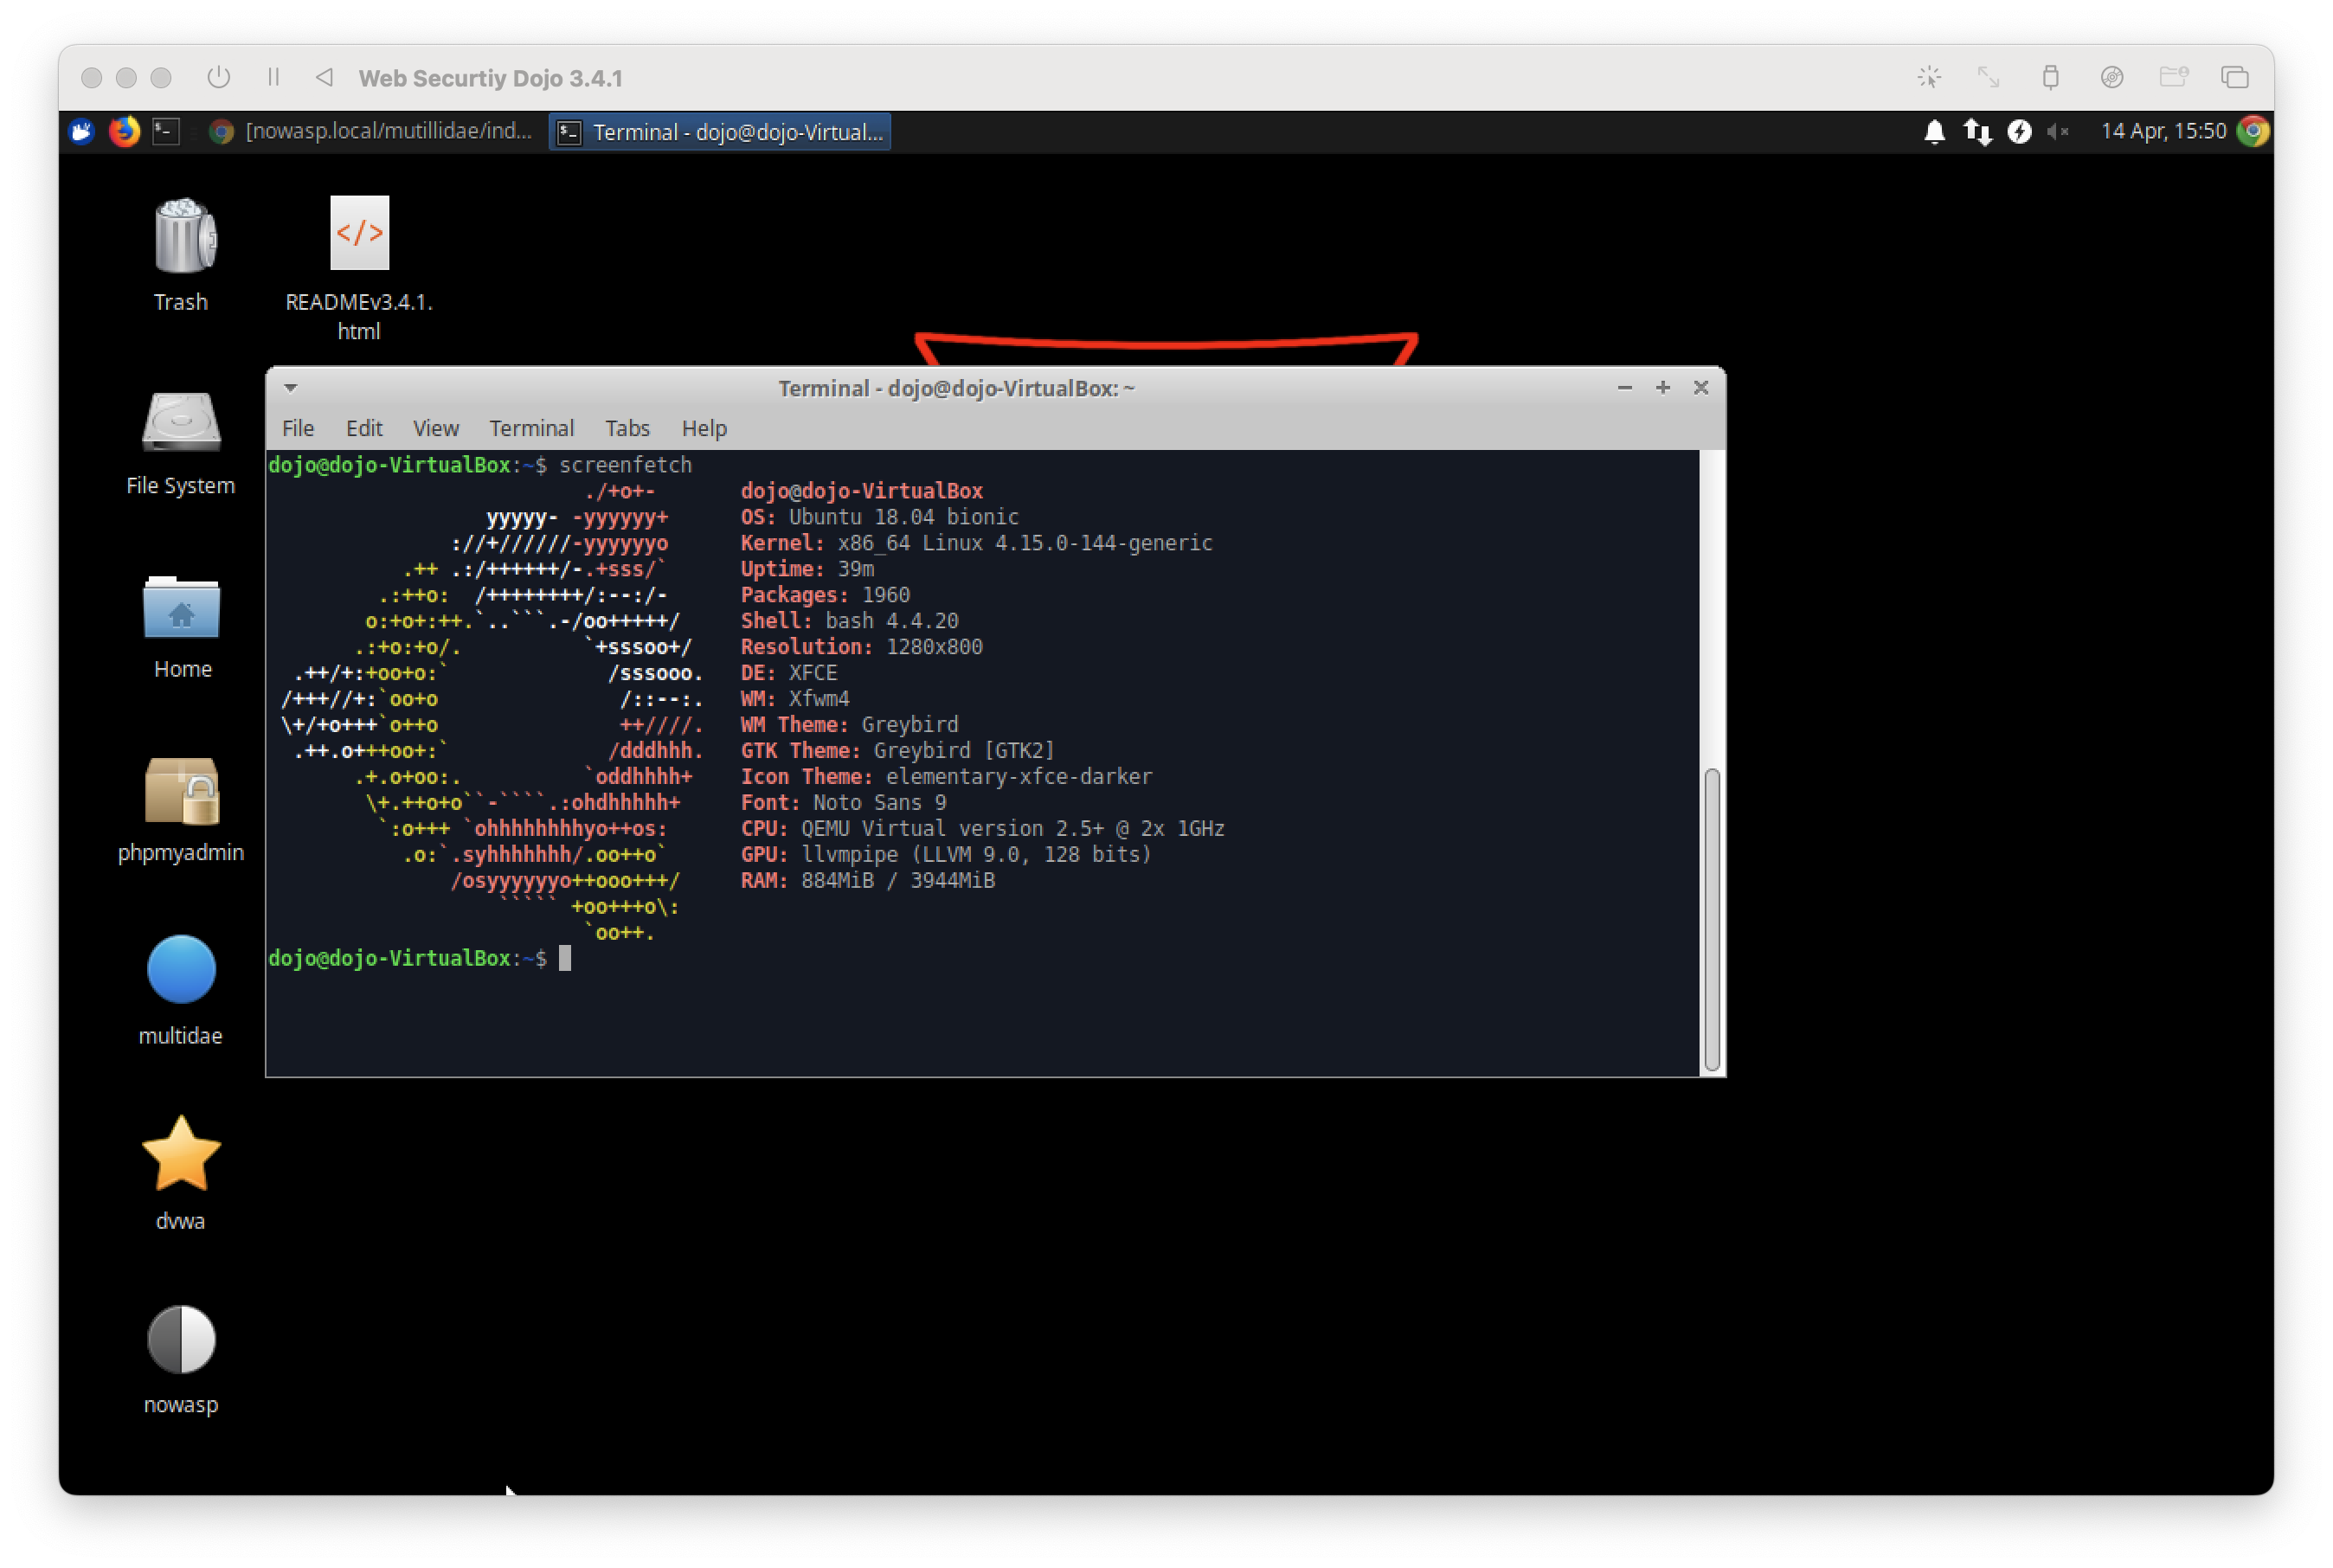
\includegraphics[width=0.8\textwidth]{step_00001}
    \caption{Запущенная виртуальная машина для эксплуатации атак}
  \end{figure}

  Чтобы не поднимать дополнительный сервер для получения и обра-ботки данных,
  полученных при помощи использования XSS атак, будем использовать уже готовую страницу,
  которая сохраняет все query-параметры и cookie, пере-данные при её запросе.

  \begin{figure}[H]
    \centering
    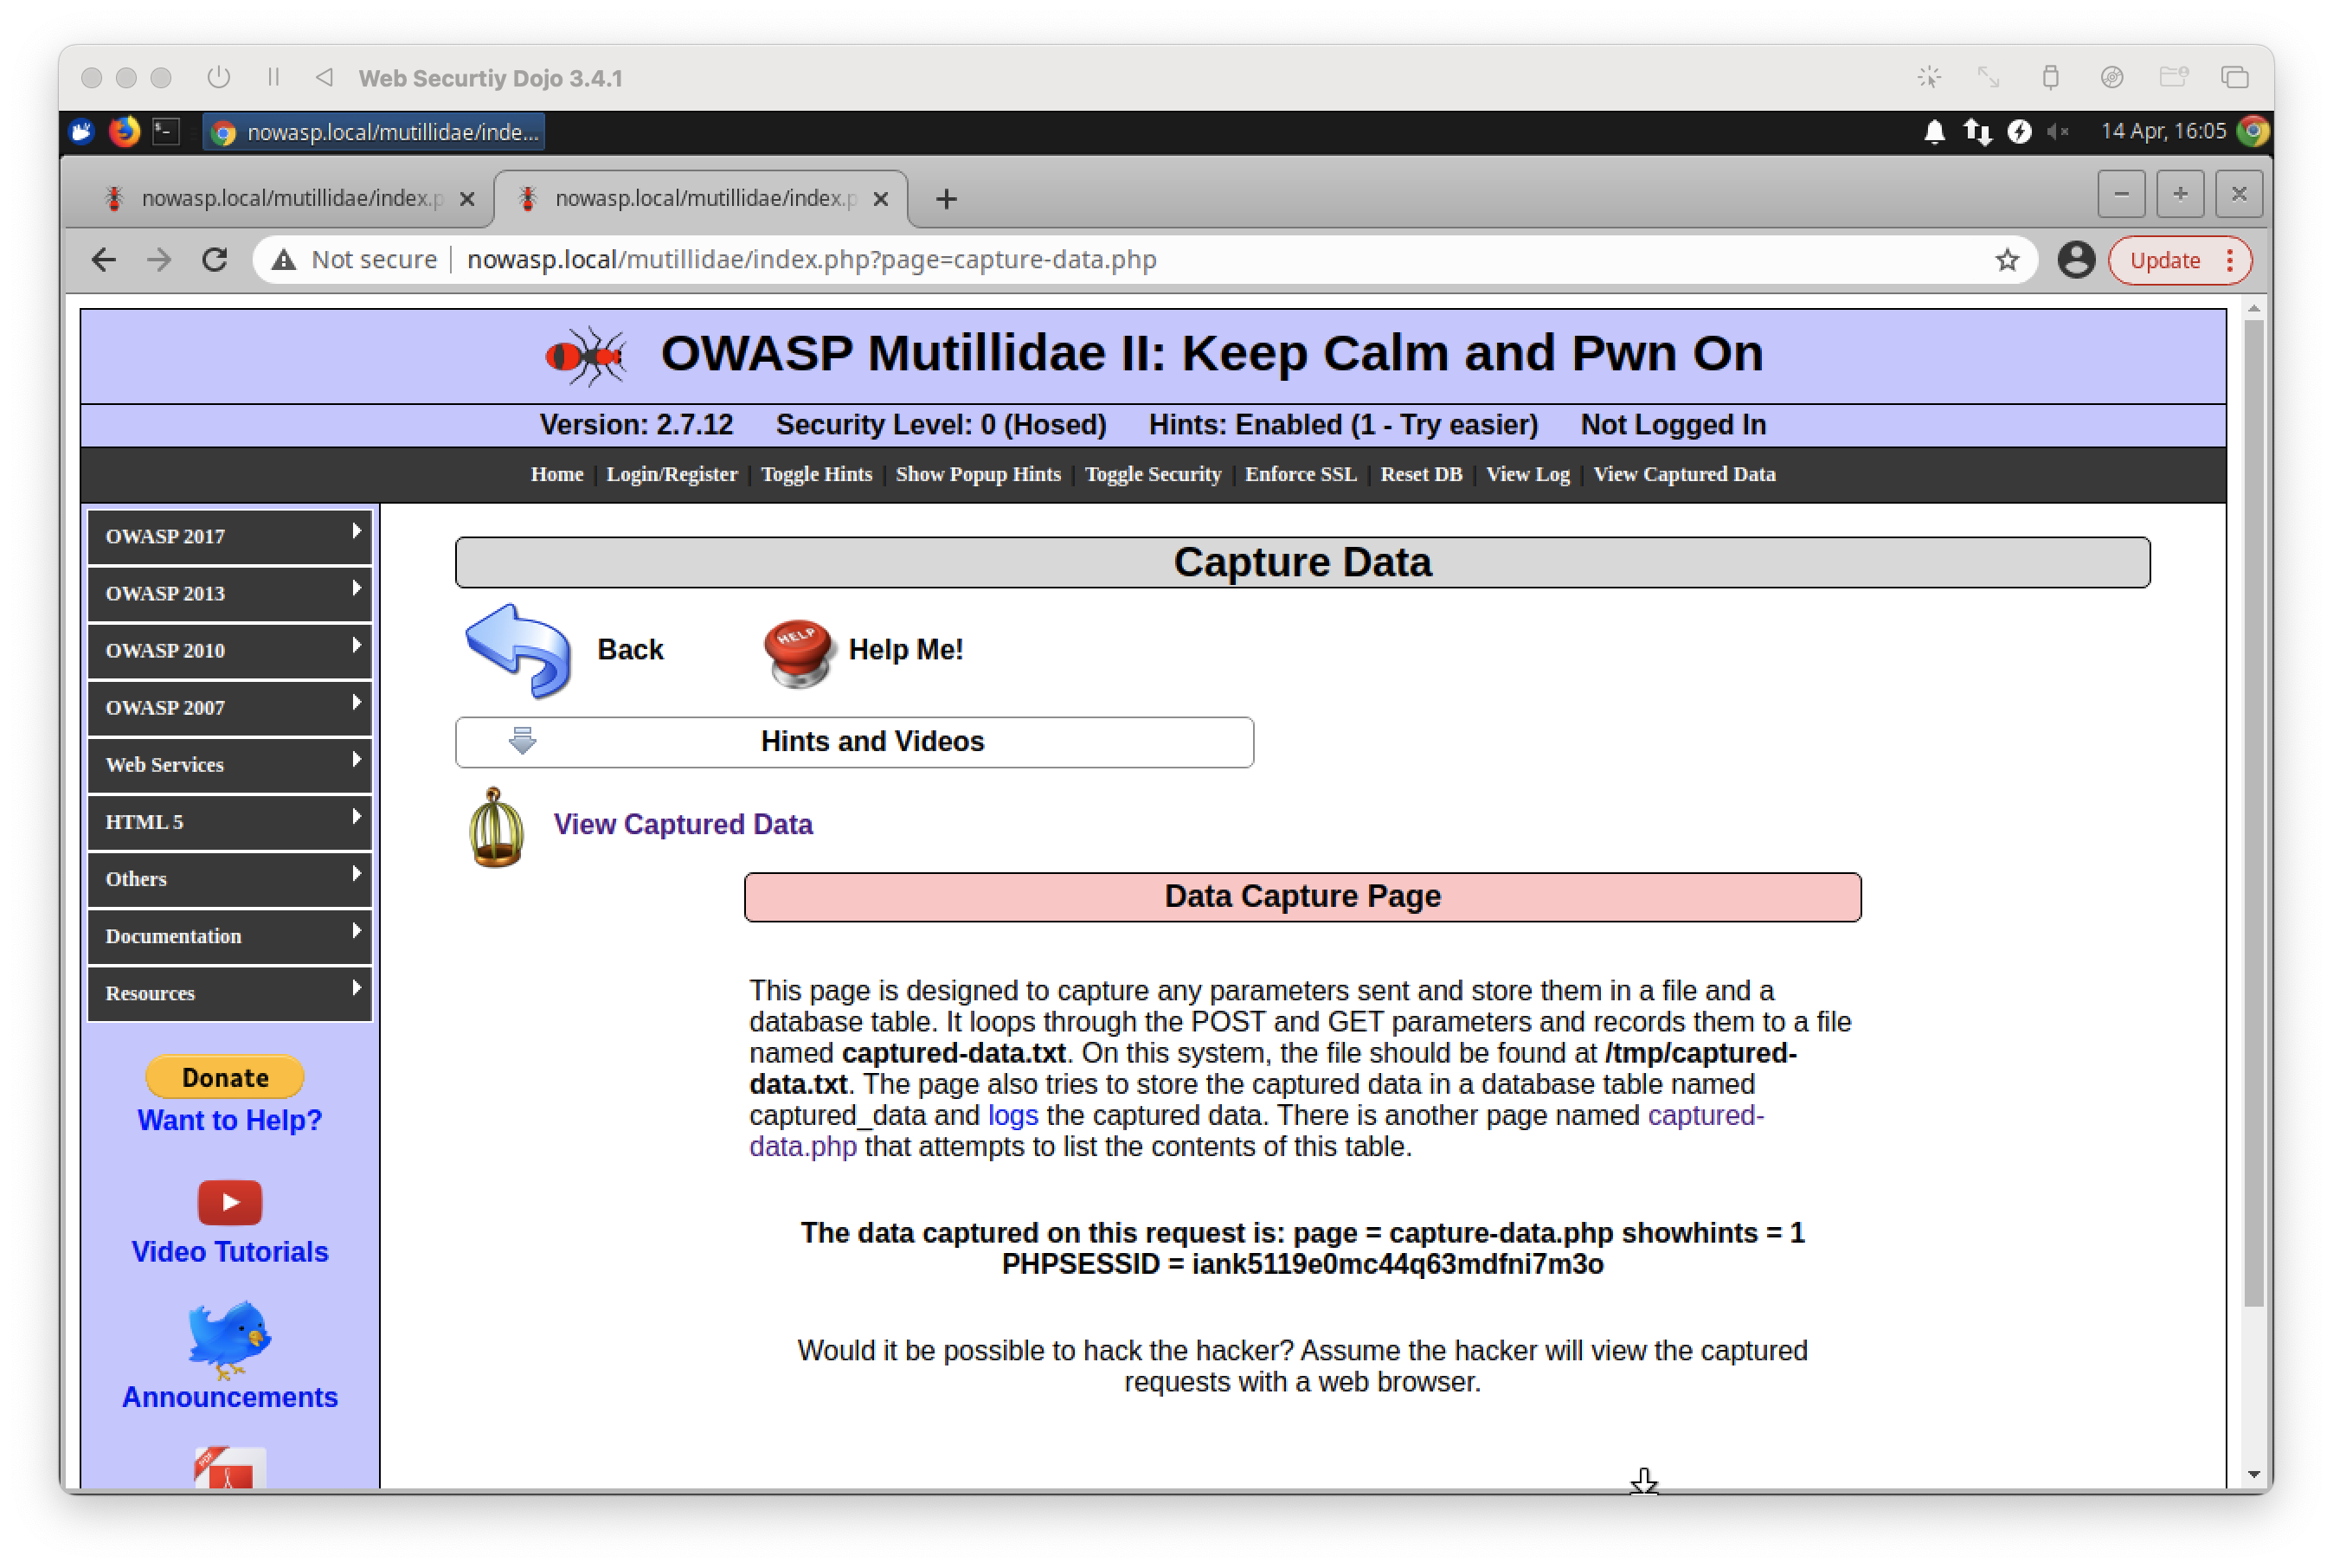
\includegraphics[width=0.8\textwidth]{step_00013}
    \caption{Страница для захвата}
  \end{figure}

  Как видим, эта страница отображает значение query-параметра page и все переданные ей
  Cookies, проверим это добавлением ещё одного аргумента:

  \begin{figure}[H]
    \centering
    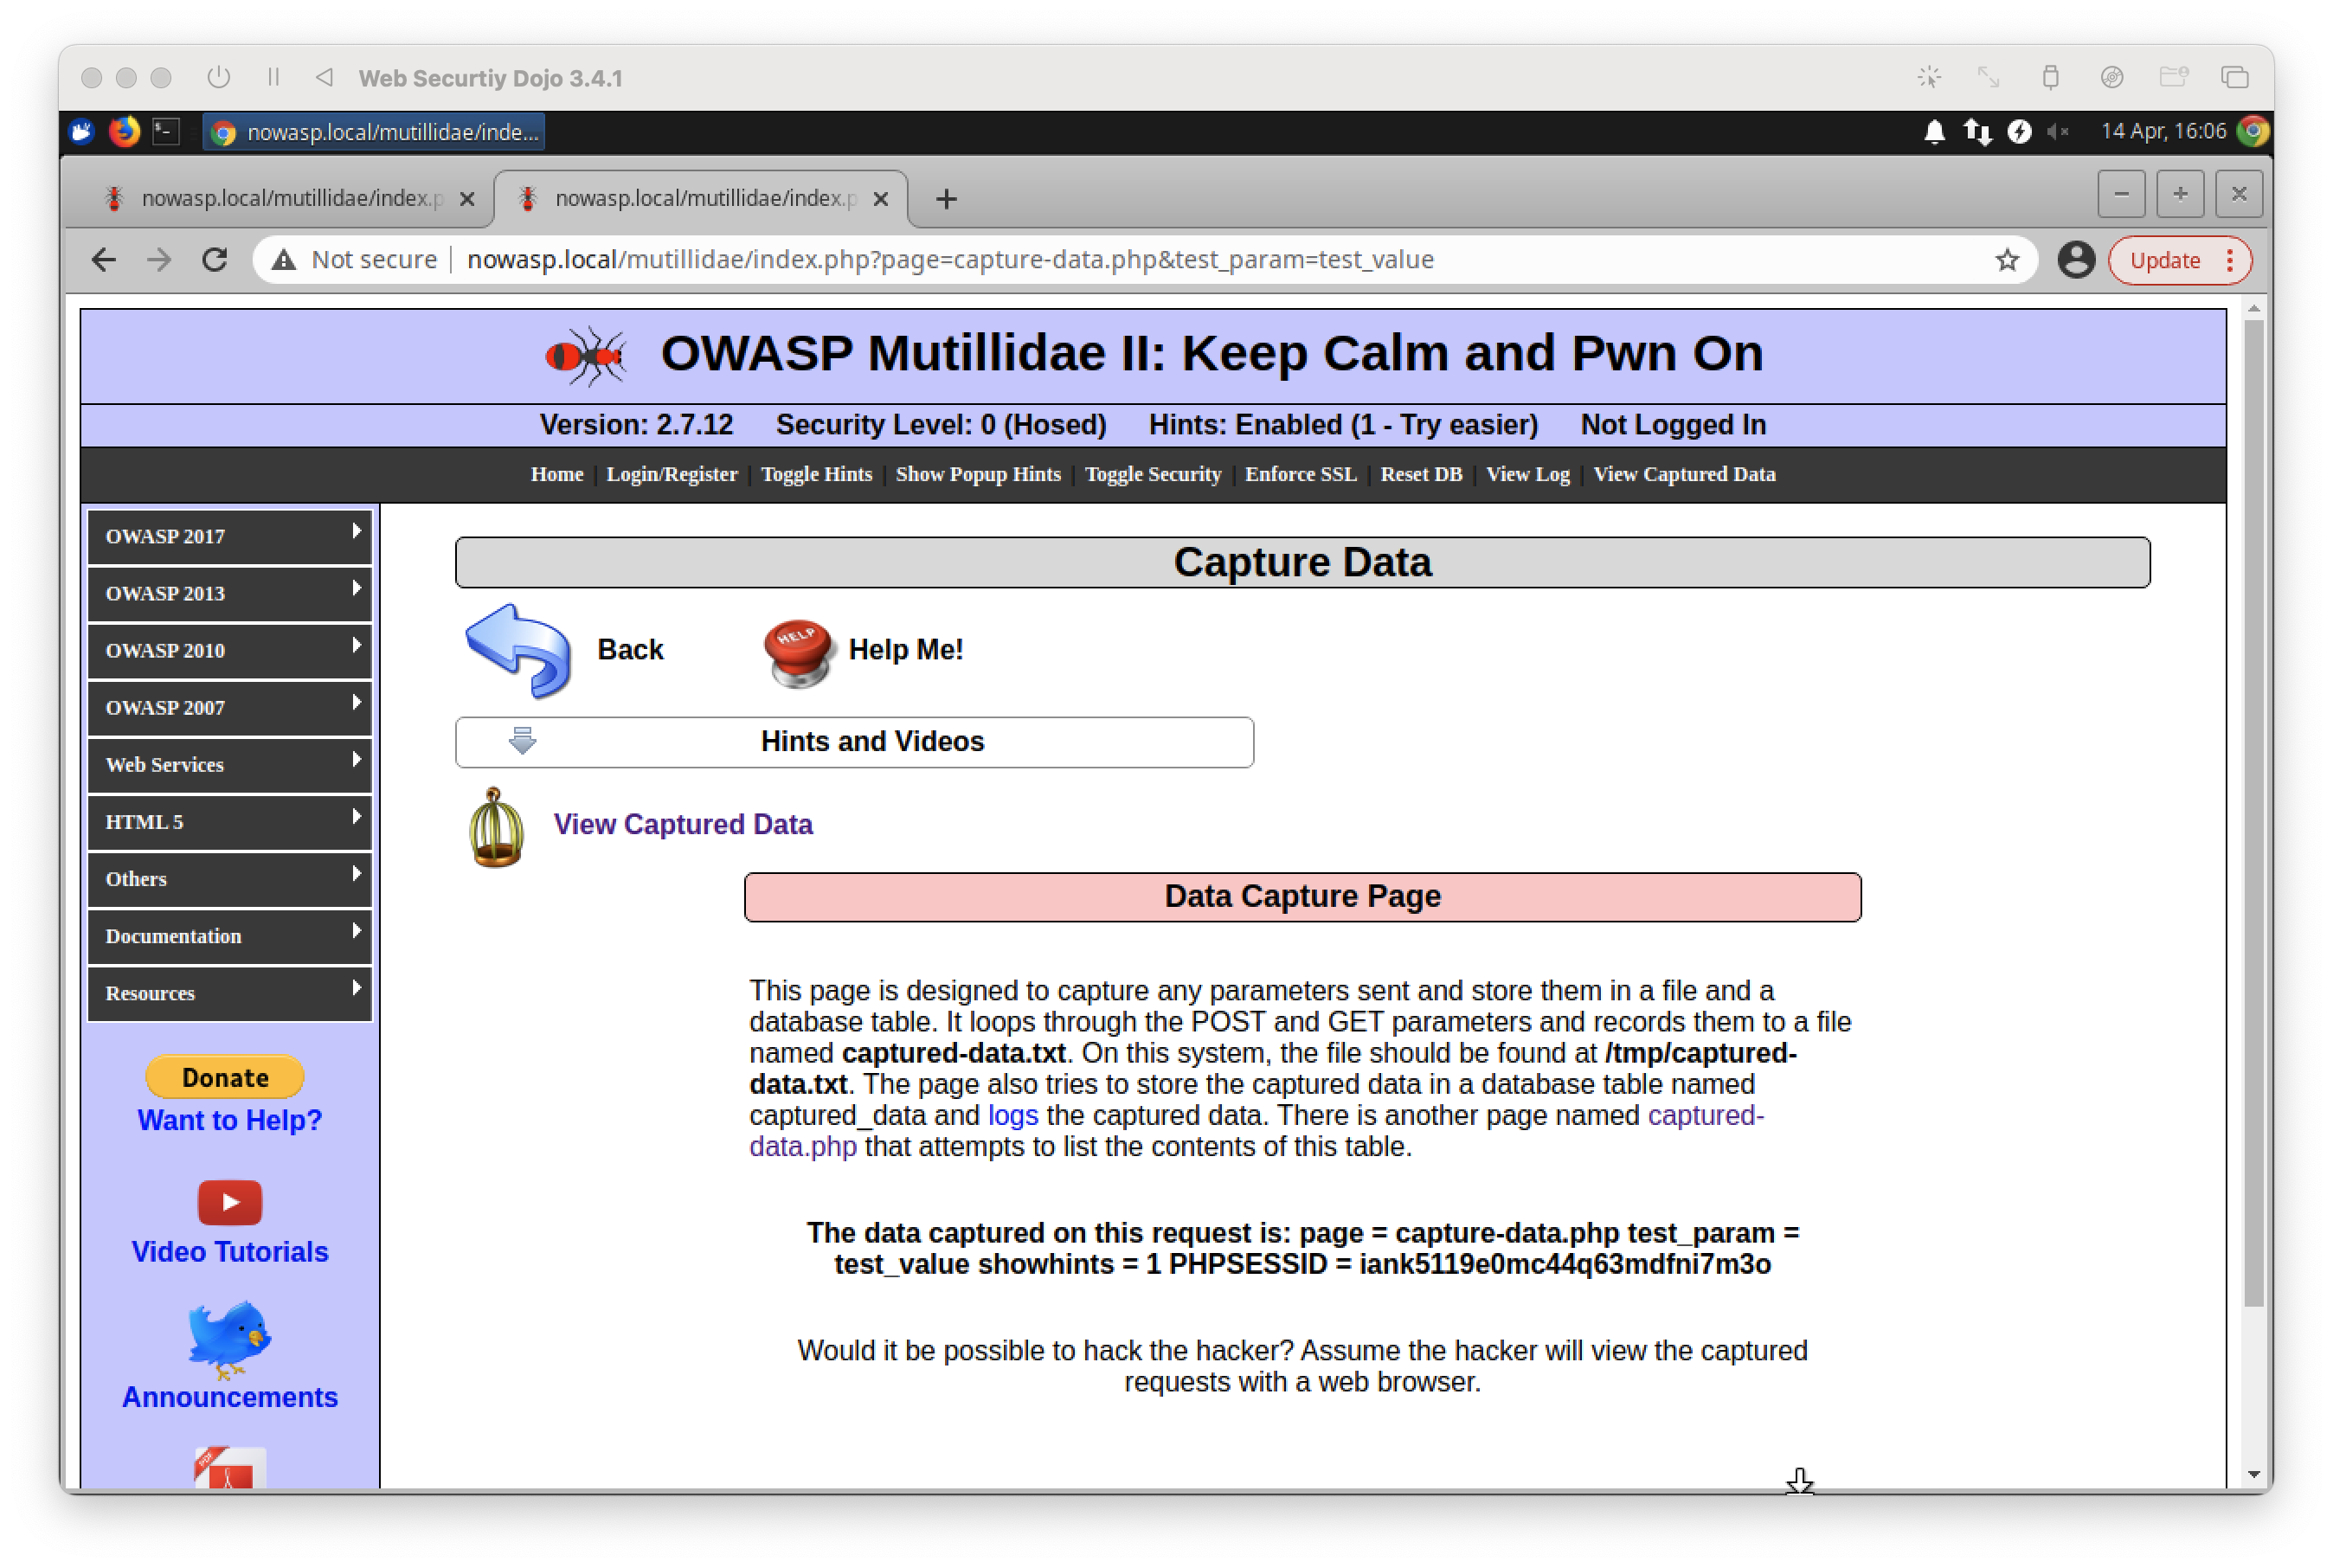
\includegraphics[width=0.8\textwidth]{step_00014}
    \caption{Страница перехватила новый query-параметр и отобразила его}
  \end{figure}

  Также есть возможность посмотреть всю историю захватов:

  \begin{figure}[H]
    \centering
    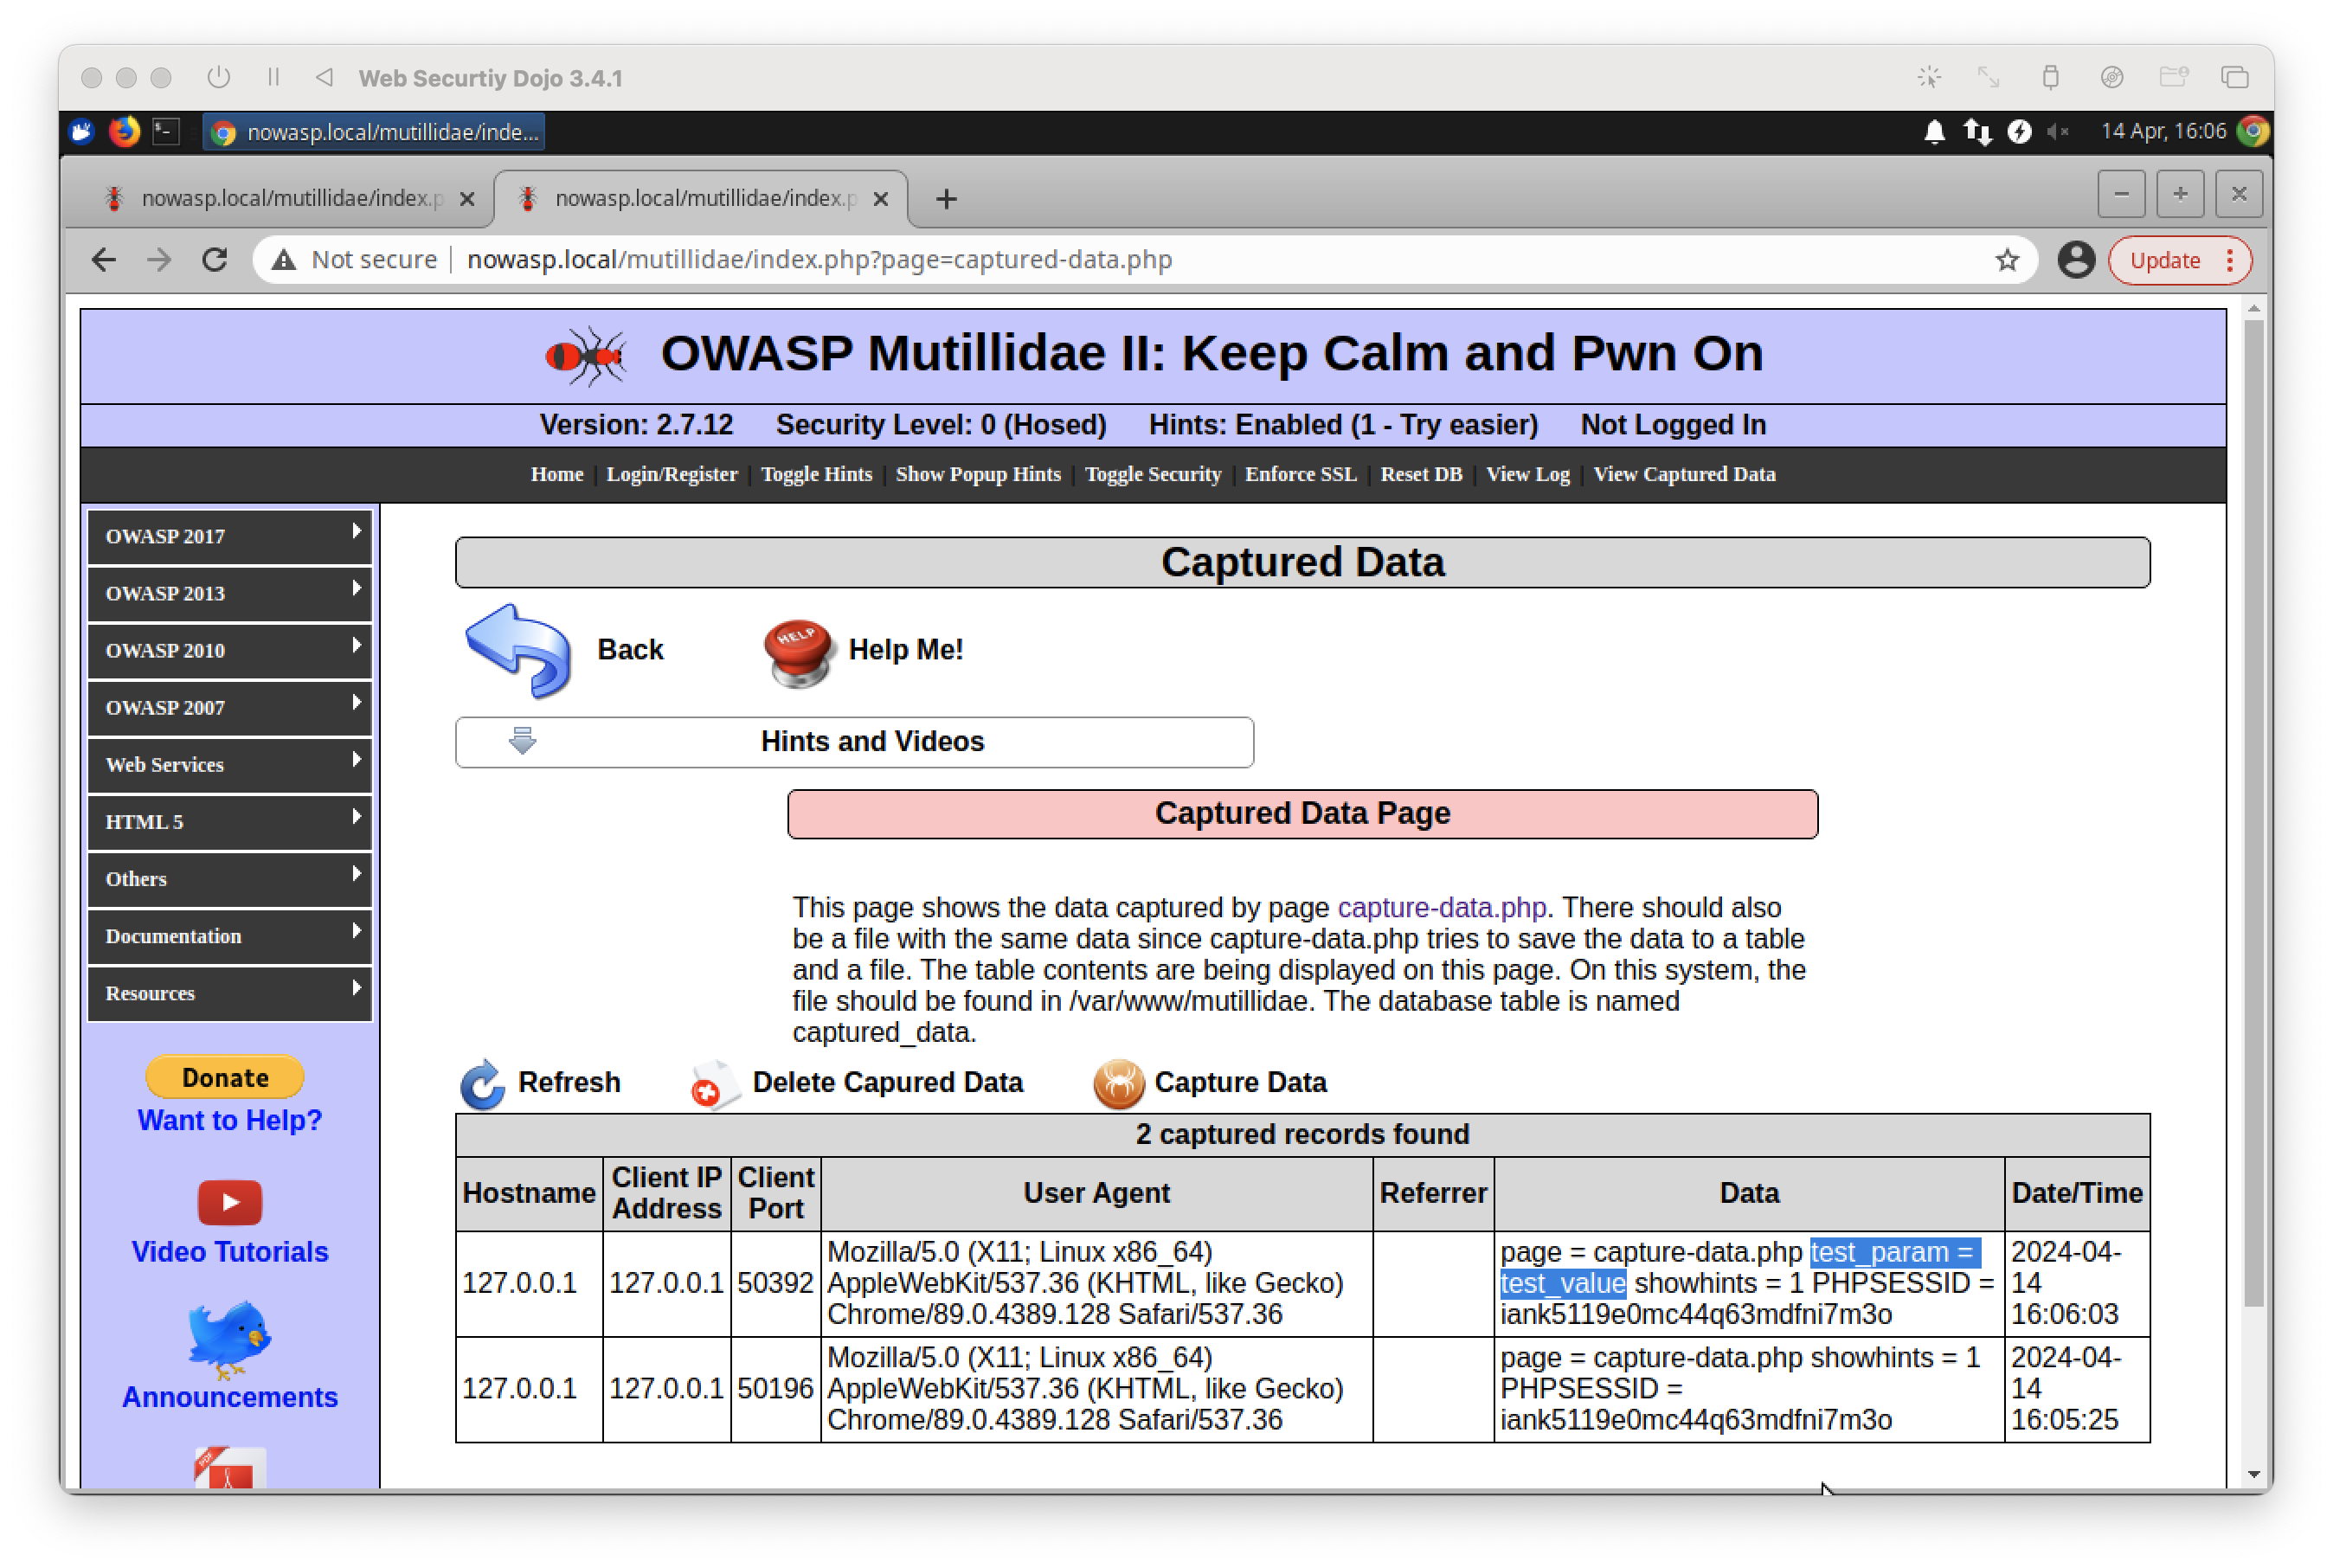
\includegraphics[width=0.8\textwidth]{step_00015}
    \caption{Страница с историей запросов к странице}
  \end{figure}

  \subsection{Reflected атака на Set Background Color}

  Открываем страницу для атаки и изучаем принцип её работы:

  \begin{figure}[H]
    \centering
    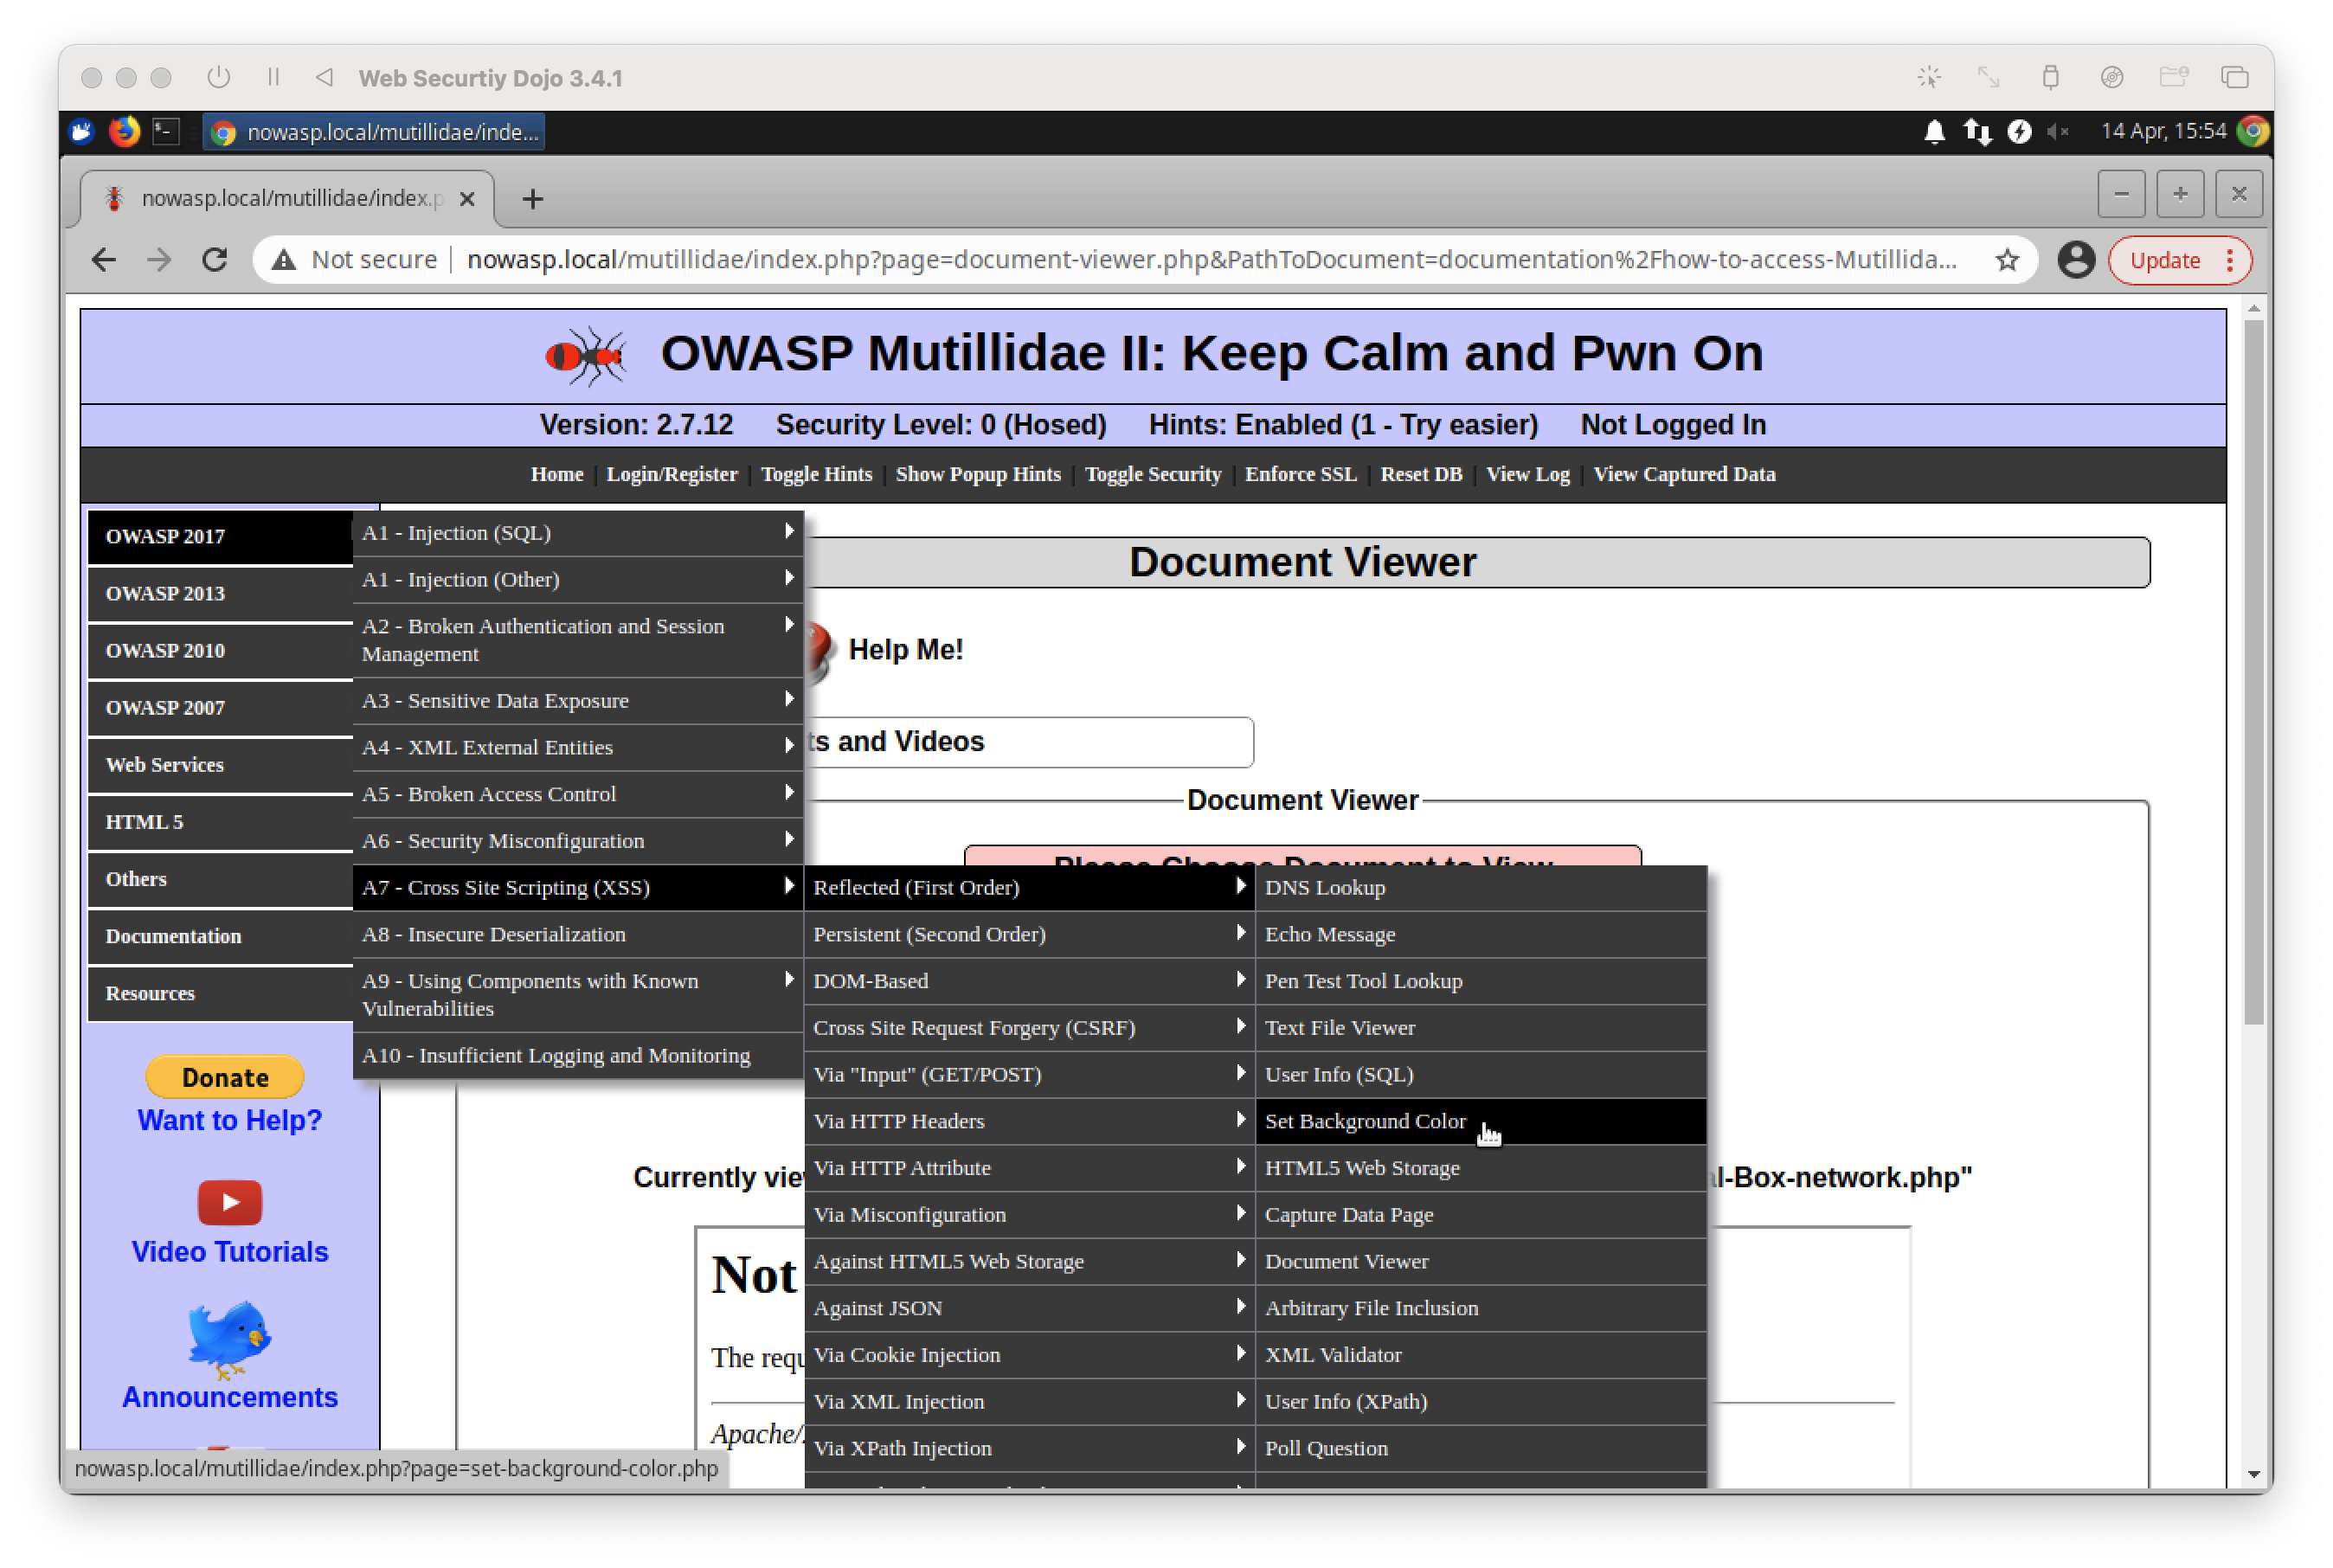
\includegraphics[width=0.8\textwidth]{step_00002}
    \caption{Расположение страницы}
  \end{figure}

  \begin{figure}[H]
    \centering
    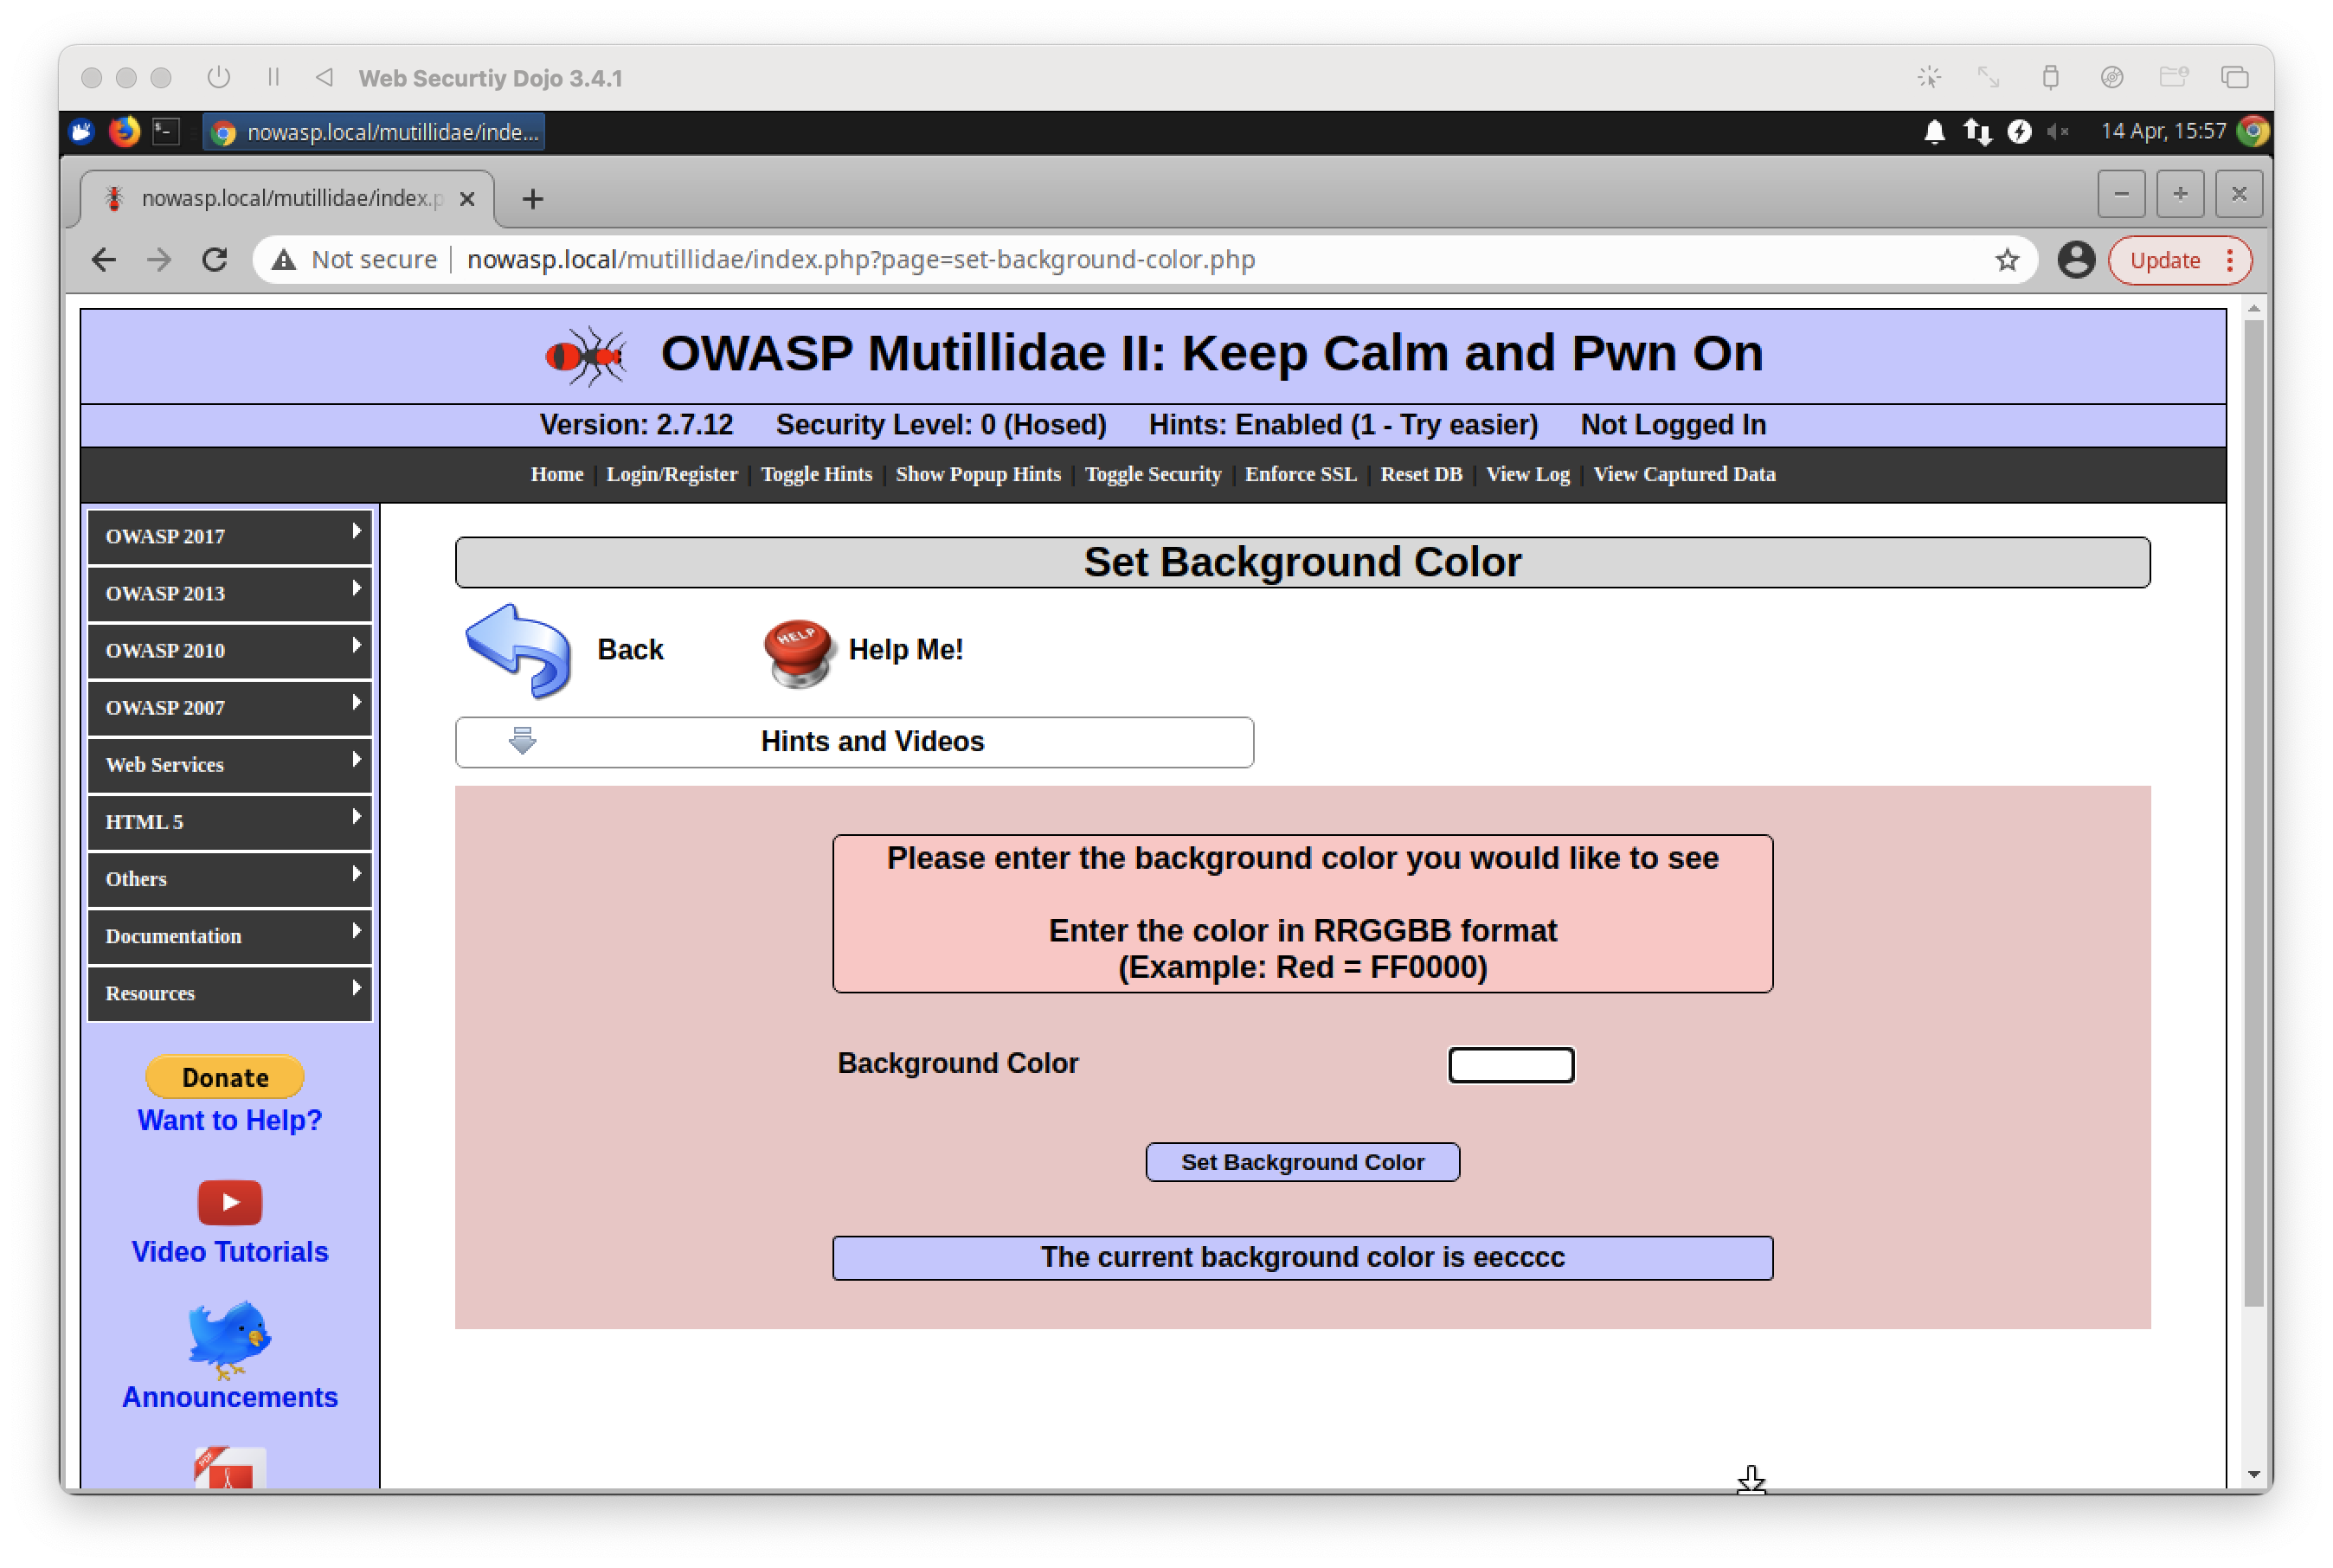
\includegraphics[width=0.8\textwidth]{step_00003}
    \caption{Сама страница}
  \end{figure}

  Судя по описанию необходимо вписать в поле ввода hex форму rgb цвета и
  фон формы изменит свой окрас на указанный:

  \begin{figure}[H]
    \centering
    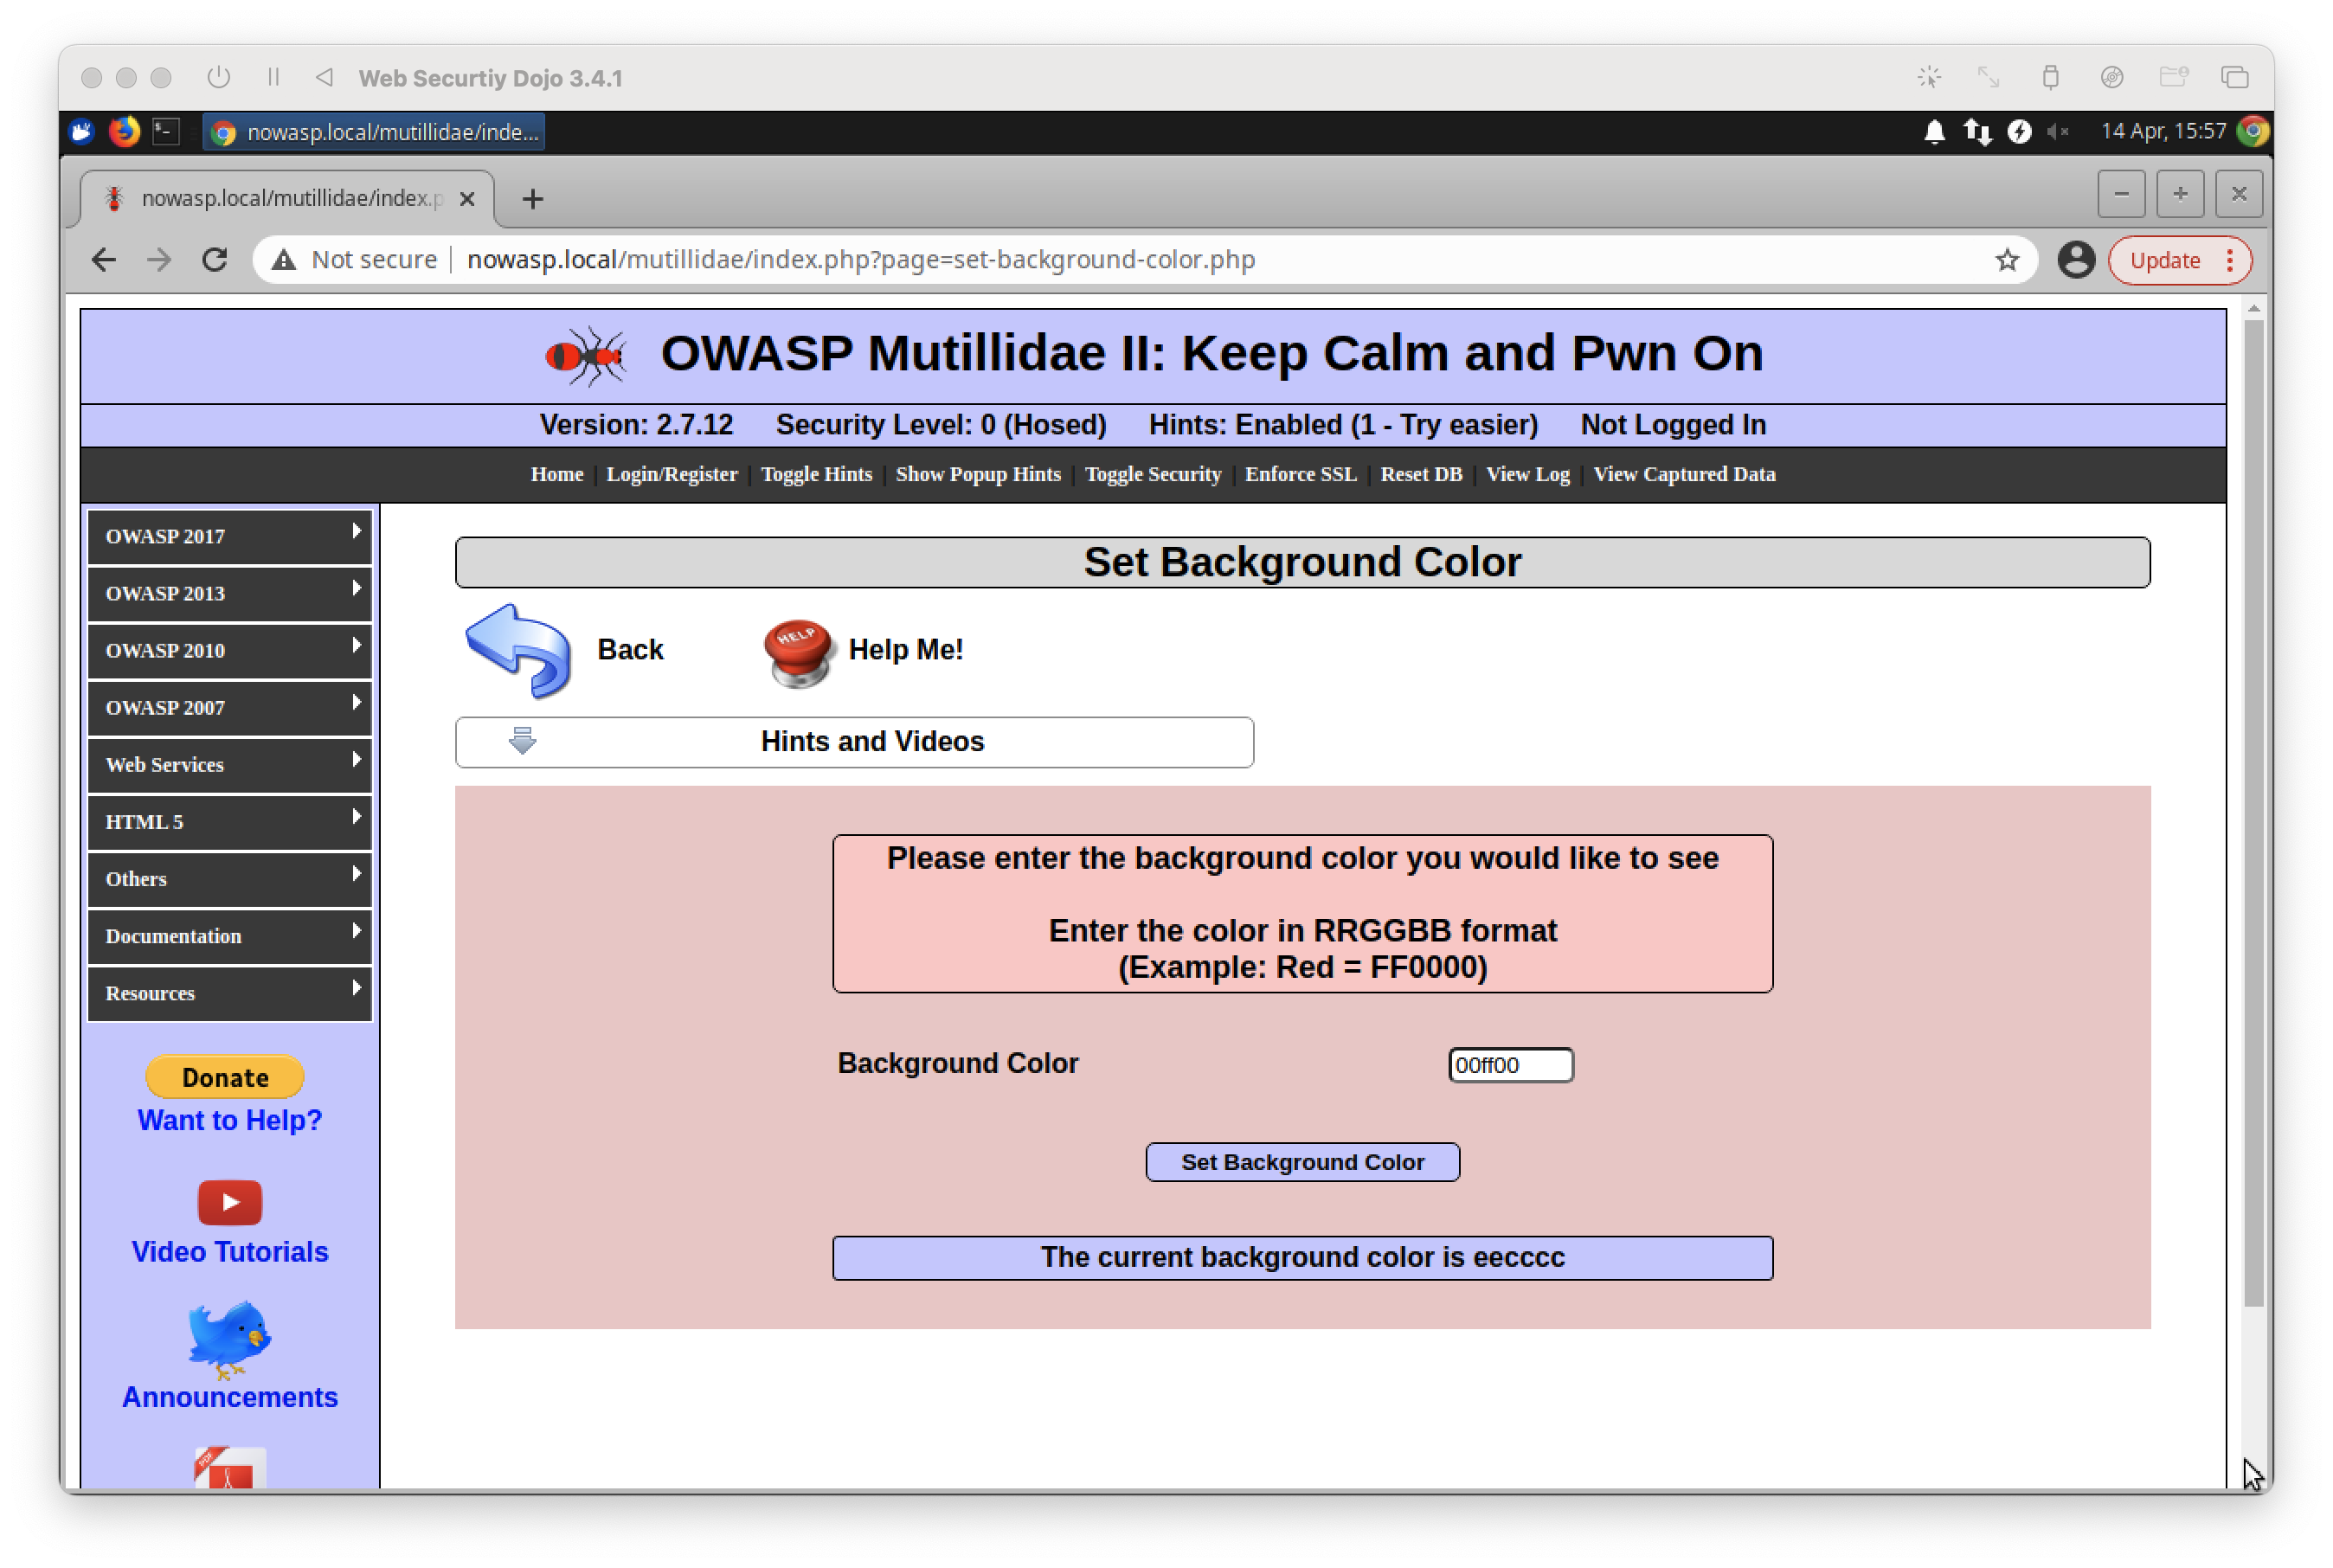
\includegraphics[width=0.8\textwidth]{step_00004}
    \caption{Попробуем установить зелёный - 00ff00}
  \end{figure}

  \begin{figure}[H]
    \centering
    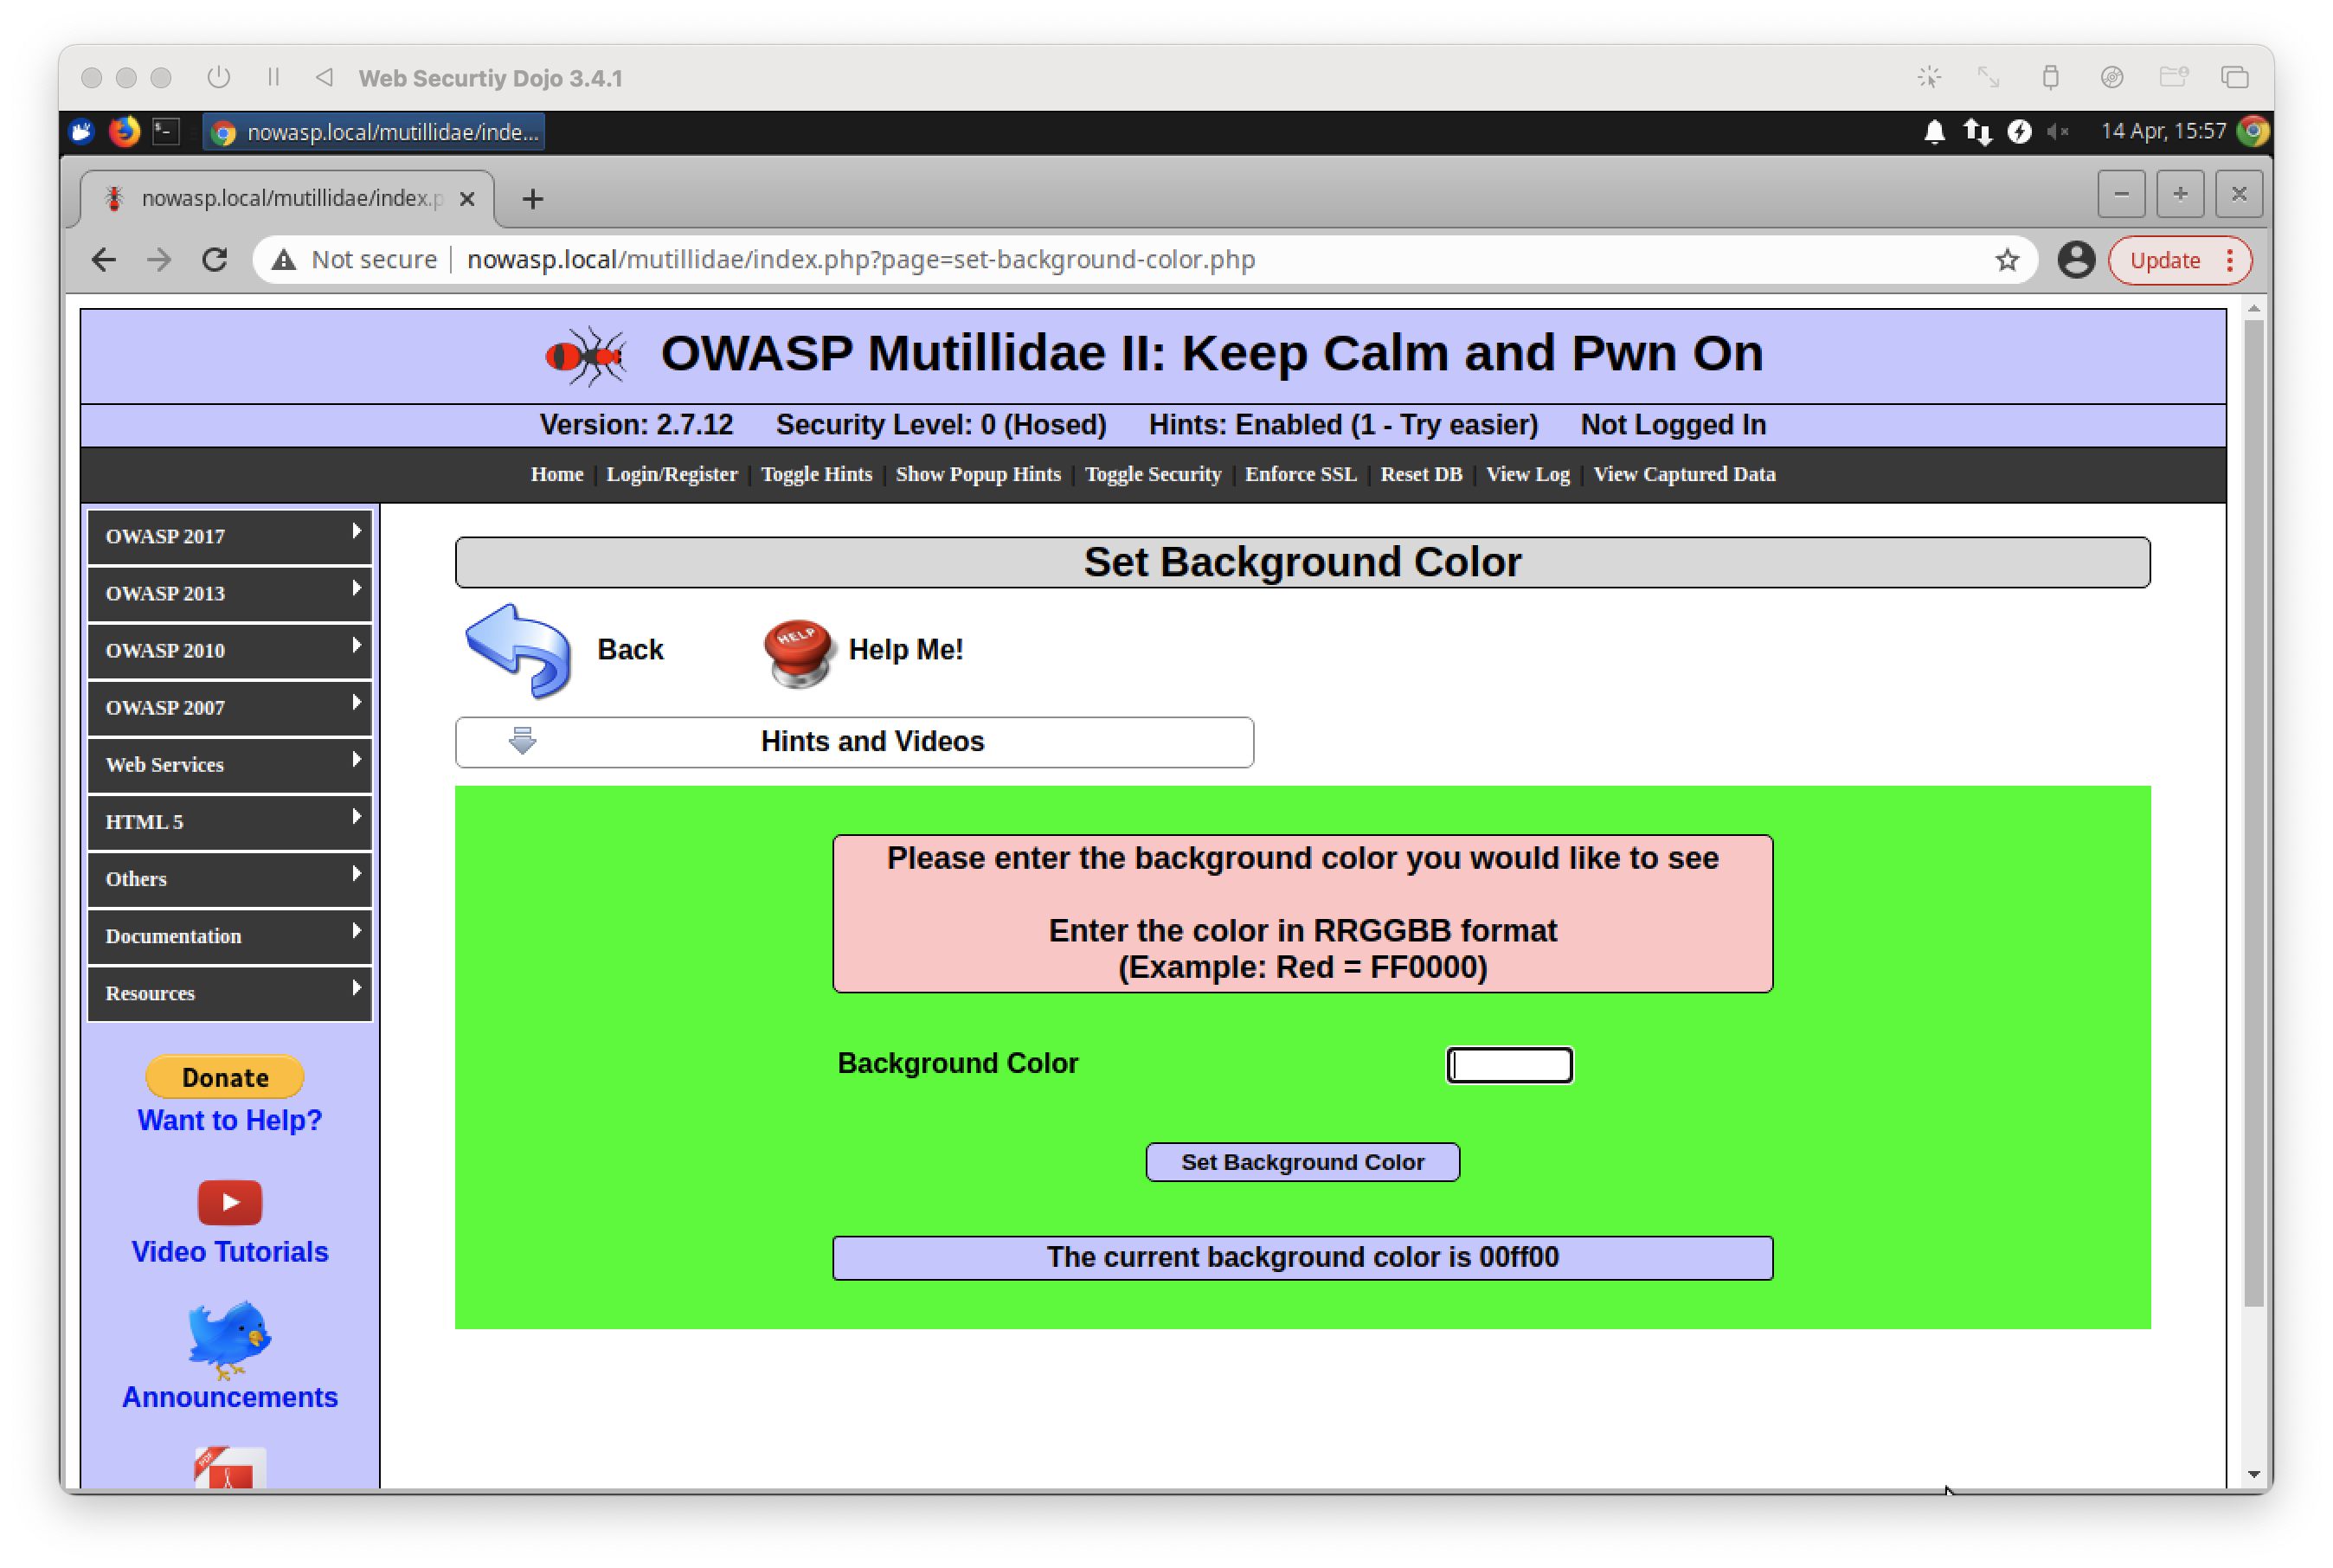
\includegraphics[width=0.8\textwidth]{step_00005}
    \caption{Цвет изменился}
  \end{figure}

  Изучим код страницы и попытаемся понять, как логика работы с цветом заливки формы
  действует изнутри:

  \begin{figure}[H]
    \centering
    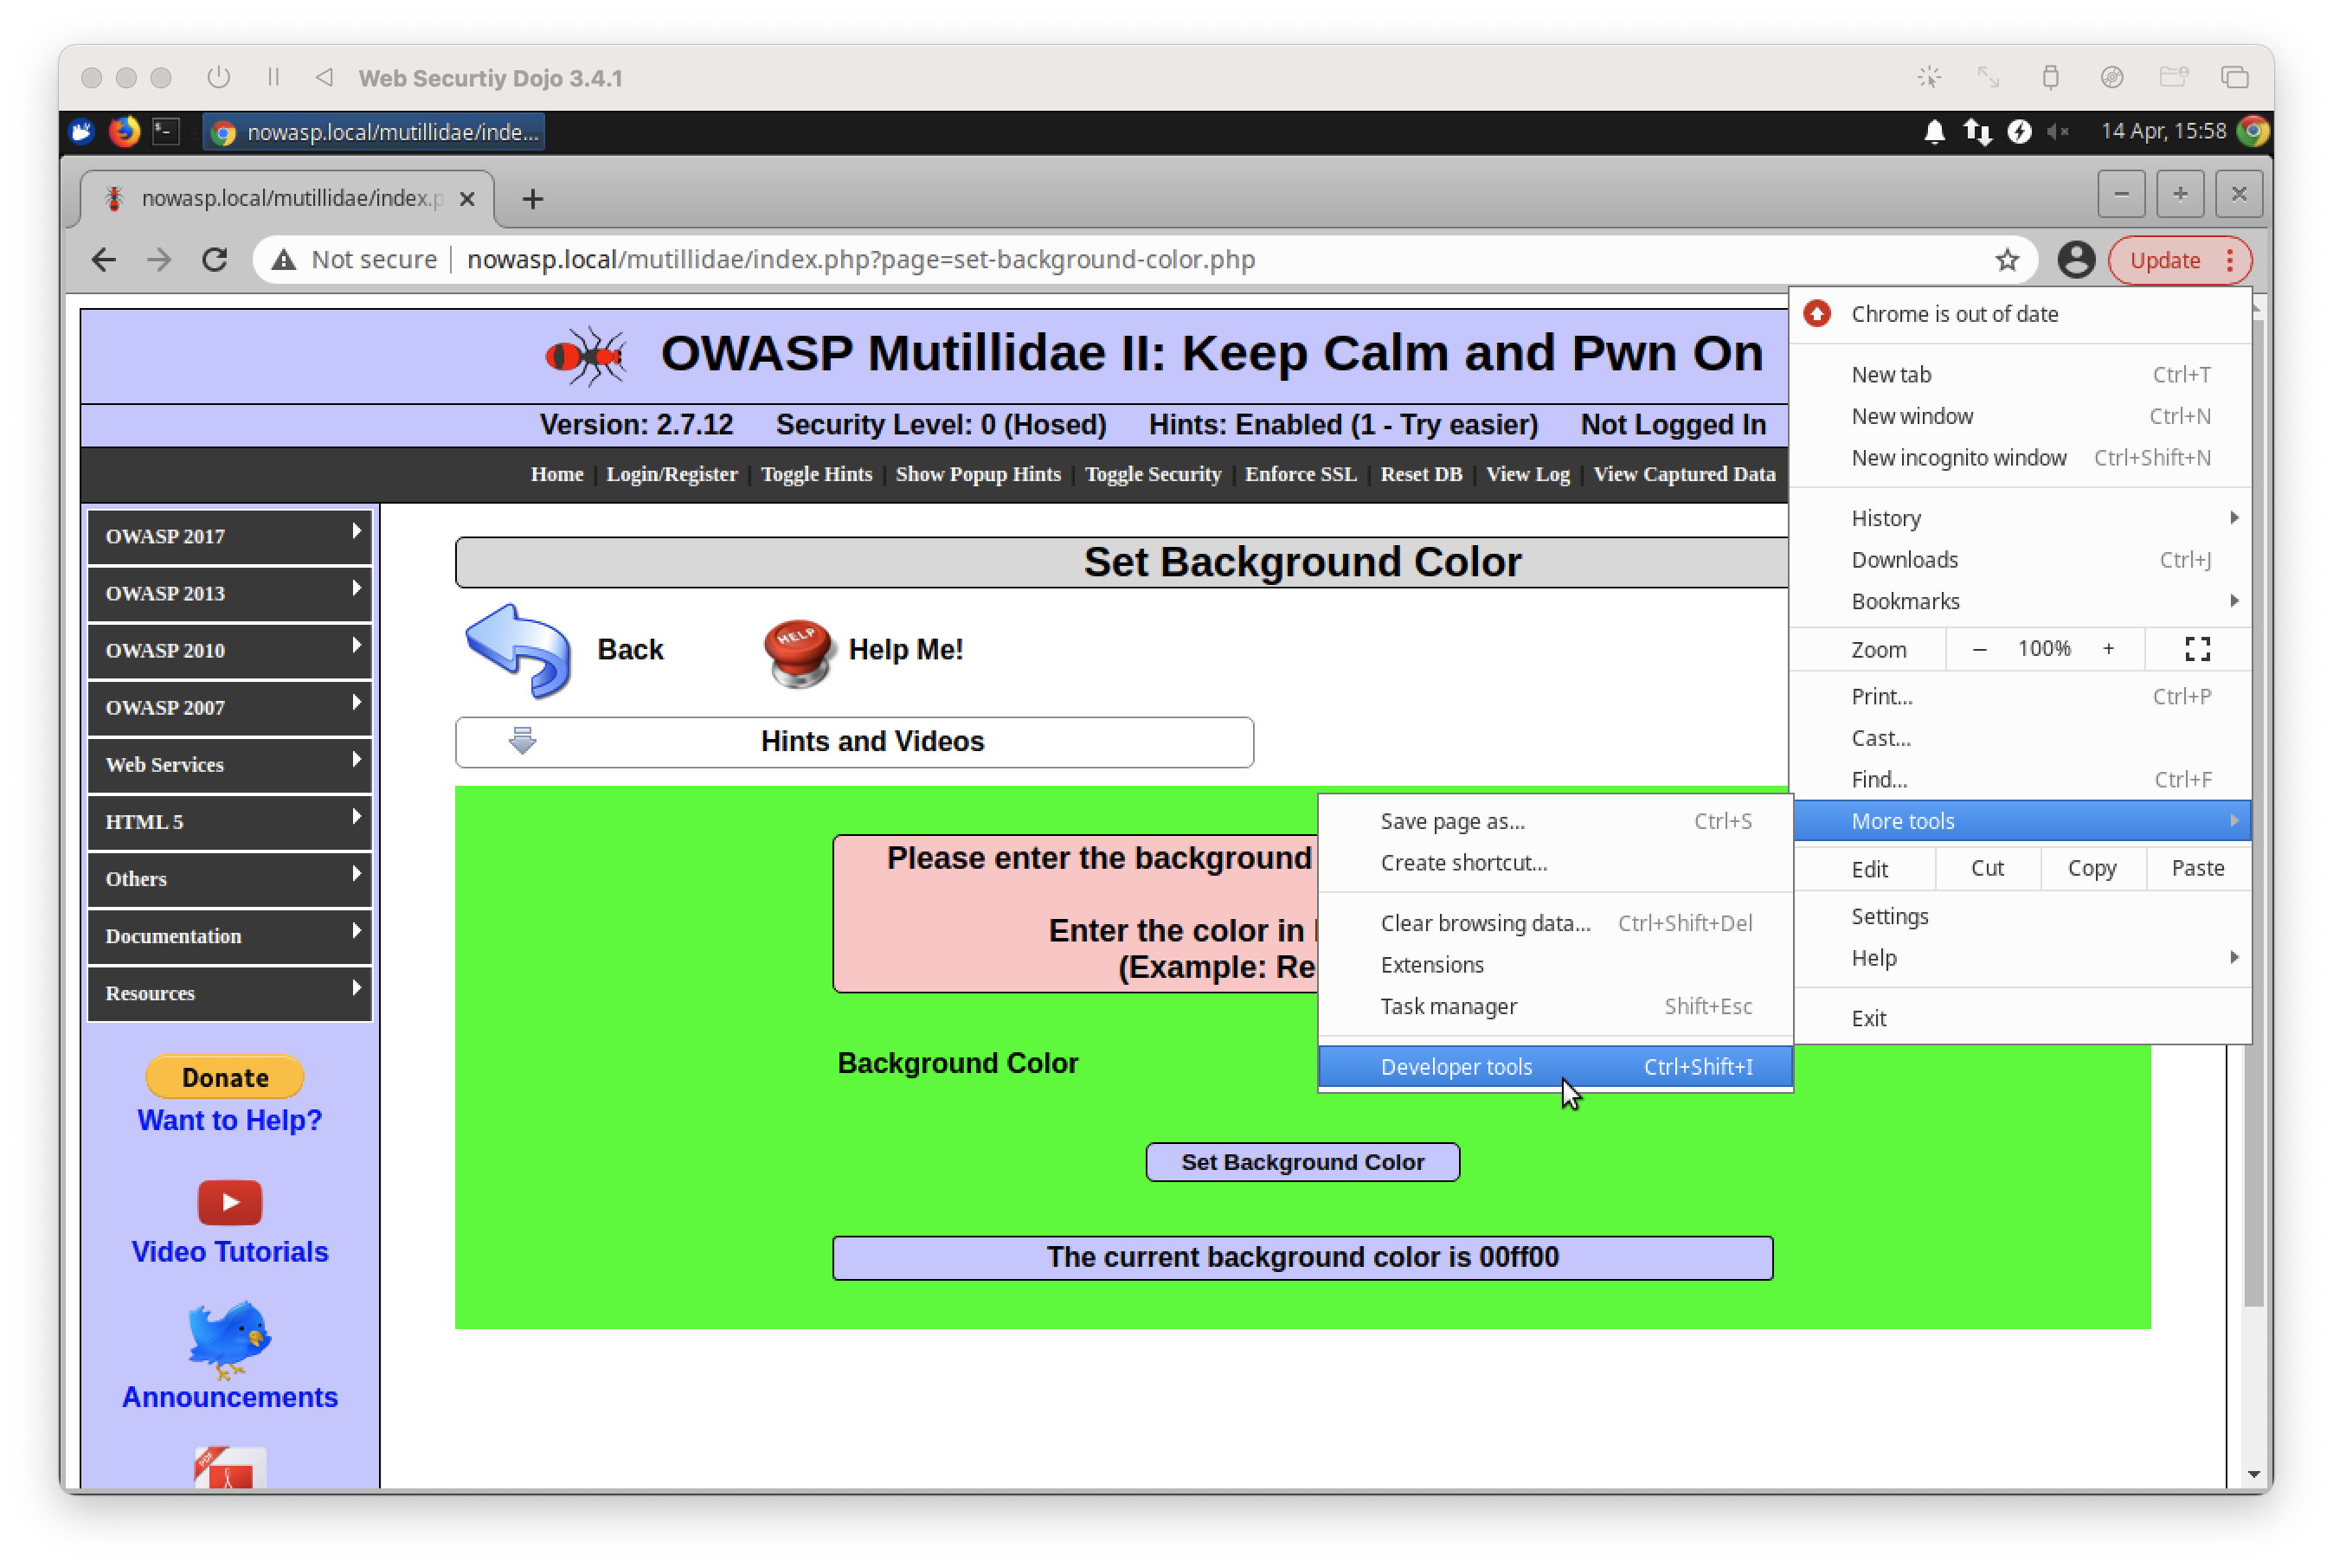
\includegraphics[width=0.8\textwidth]{step_00006}
    \caption{Запускаем инструменты разработчика}
  \end{figure}

  \begin{figure}[H]
    \centering
    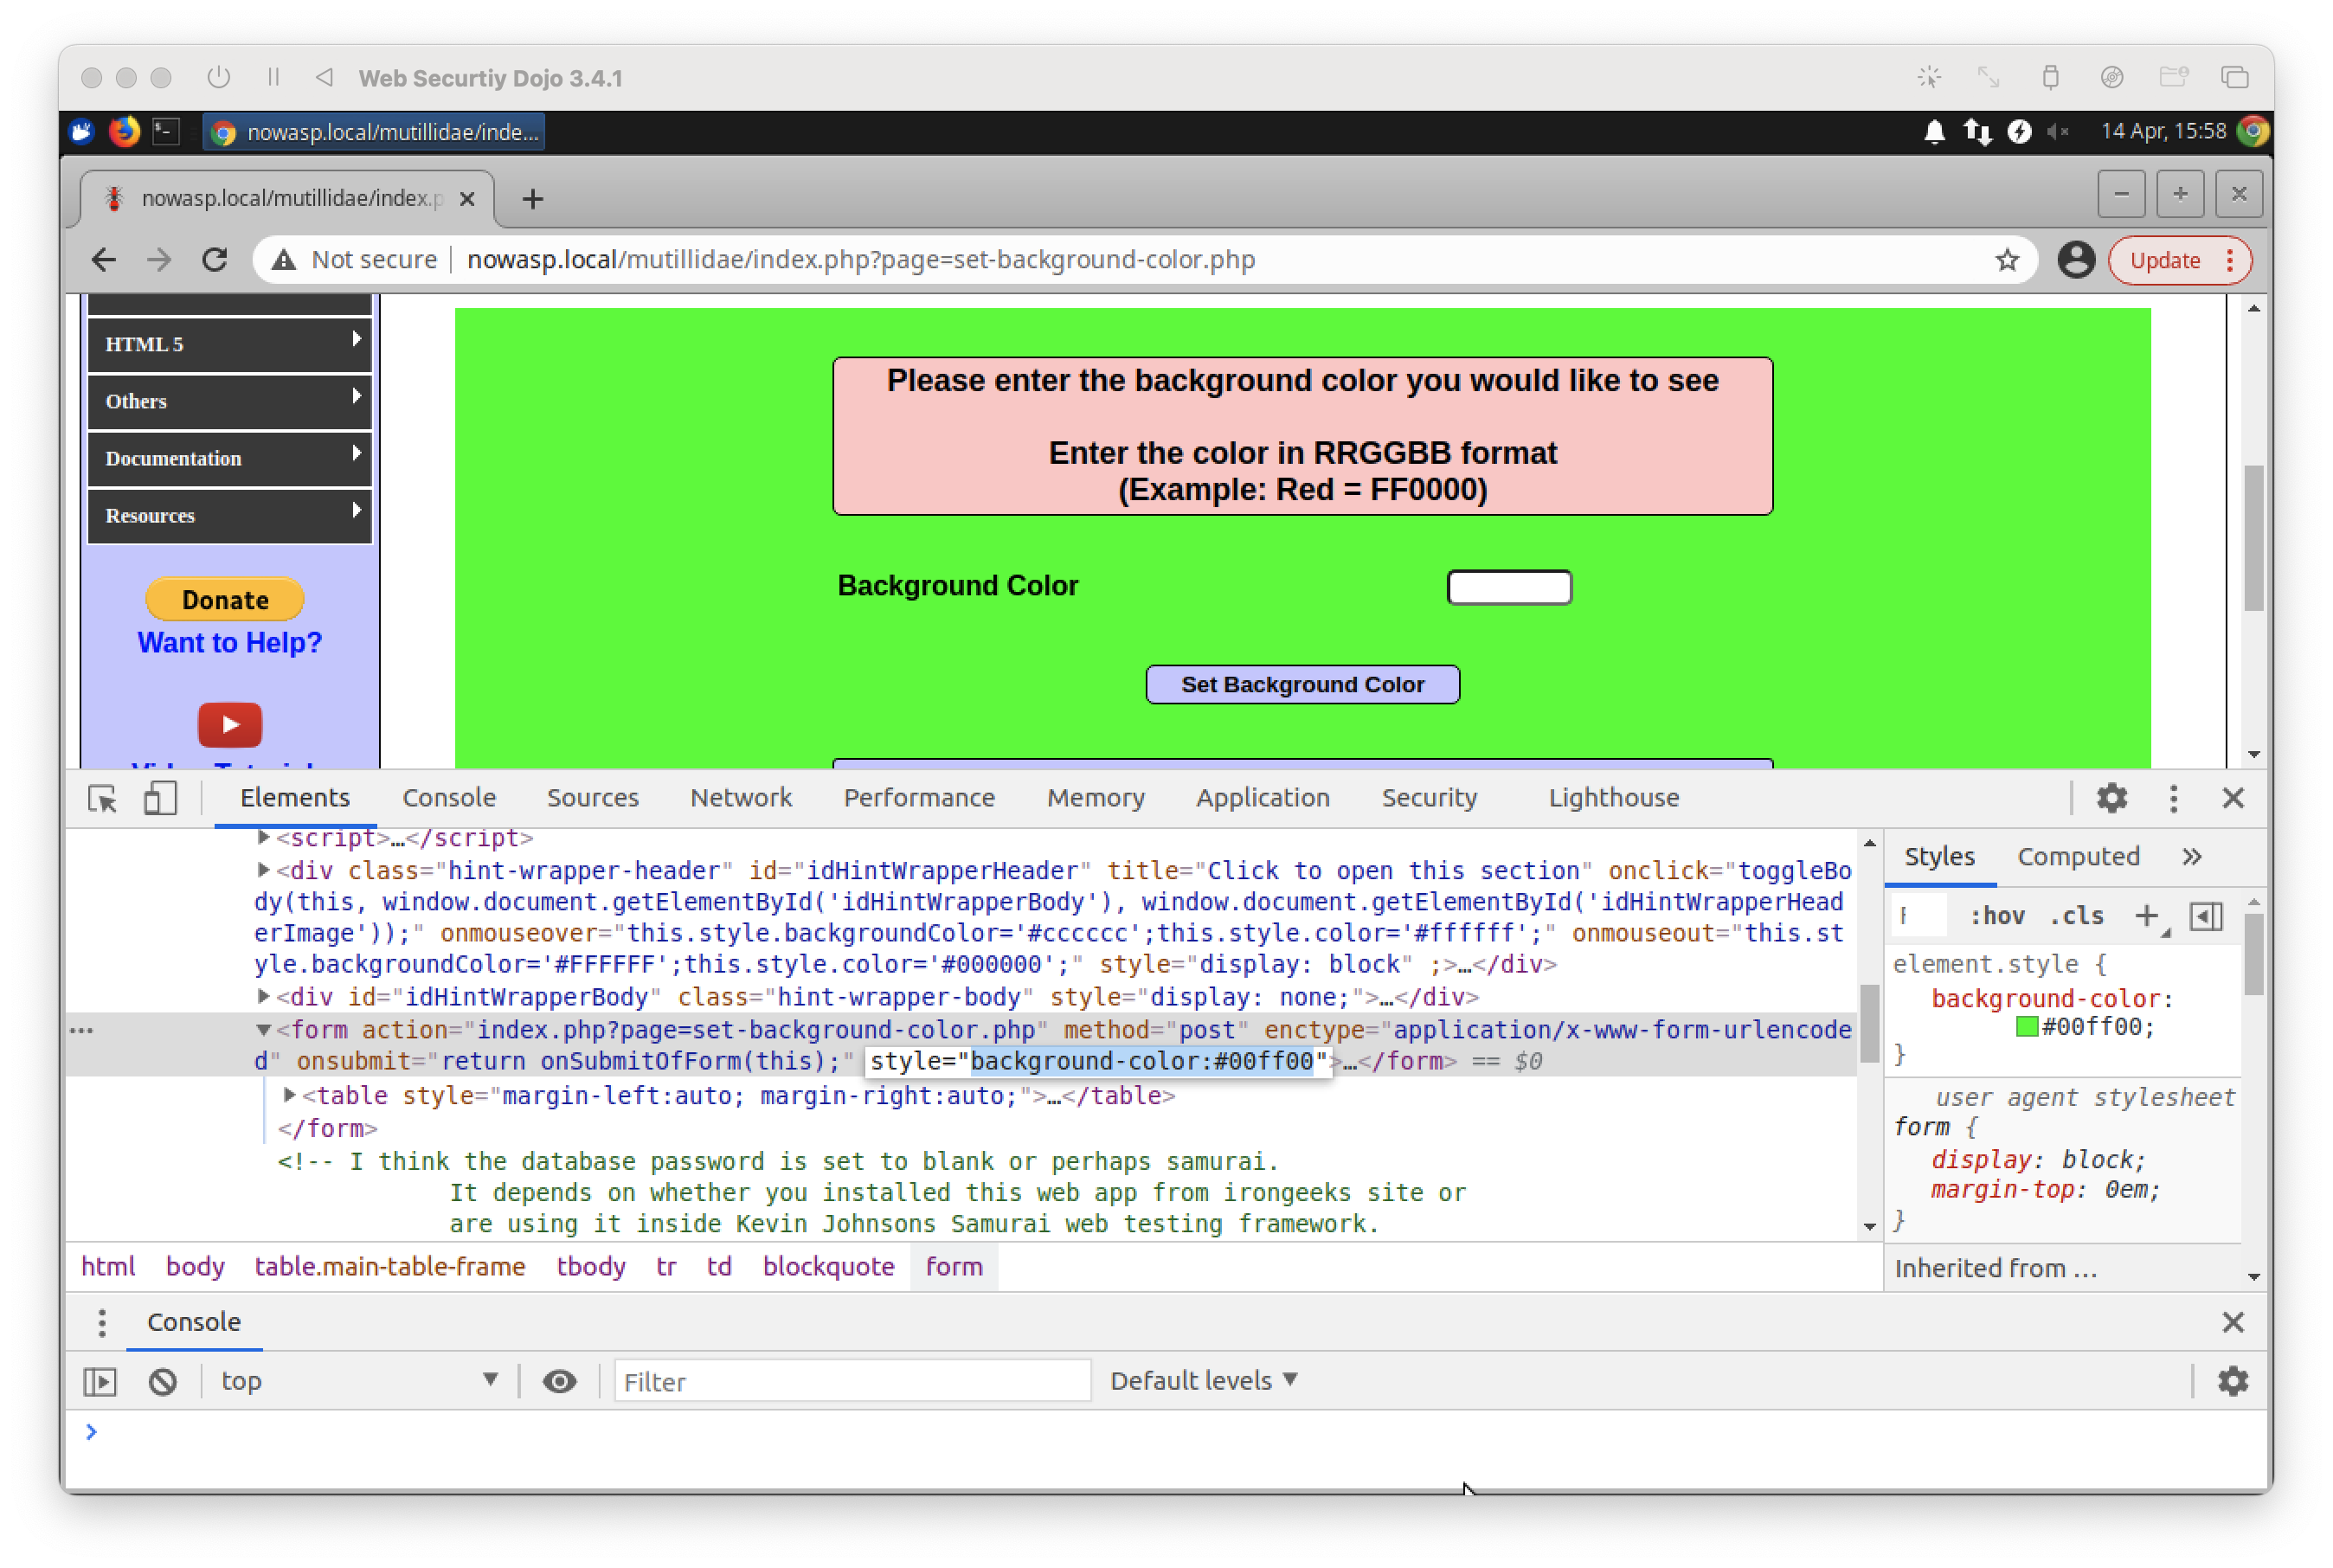
\includegraphics[width=0.8\textwidth]{step_00007}
    \caption{Видим указанный нами цвет}
  \end{figure}

  Он проставился как значение css параметра background-color. Попробуем записать
  сюда что-то, что не является hex представлением цвета из пространст-ва rgb:

  \begin{figure}[H]
    \centering
    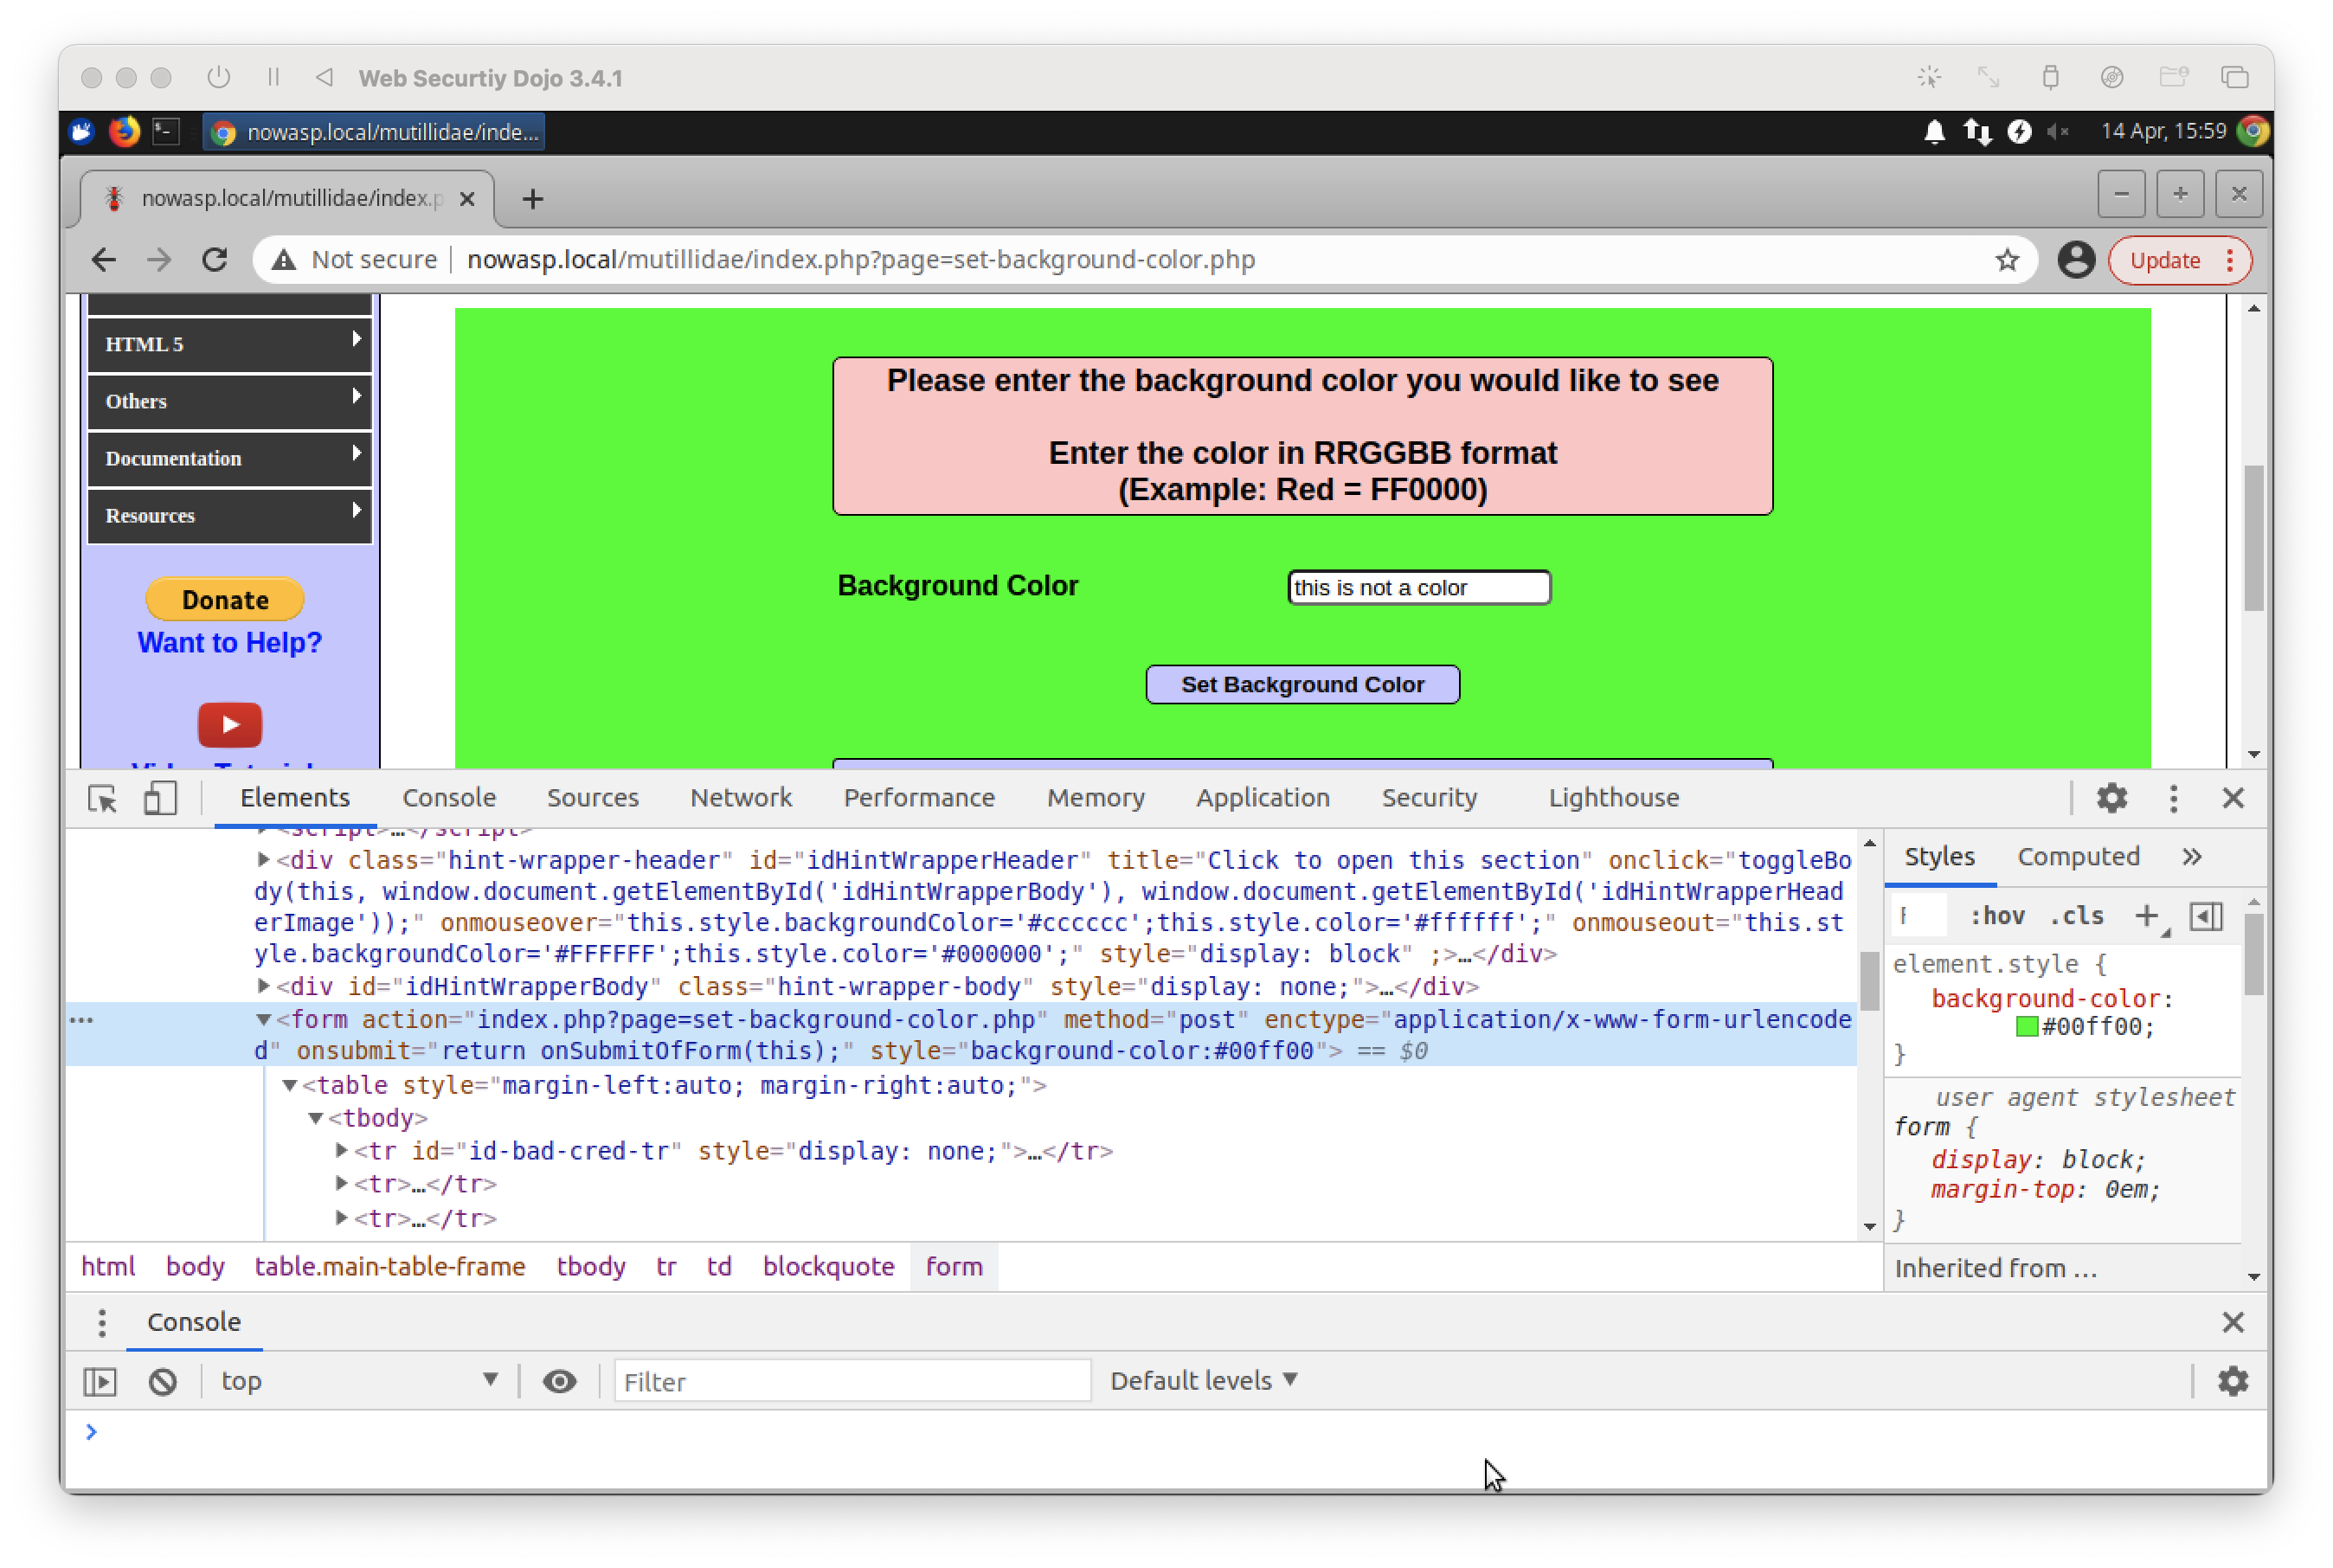
\includegraphics[width=0.8\textwidth]{step_00008}
    \caption{Вводим невалидный цвет (совсем не цвет)}
  \end{figure}

  \begin{figure}[H]
    \centering
    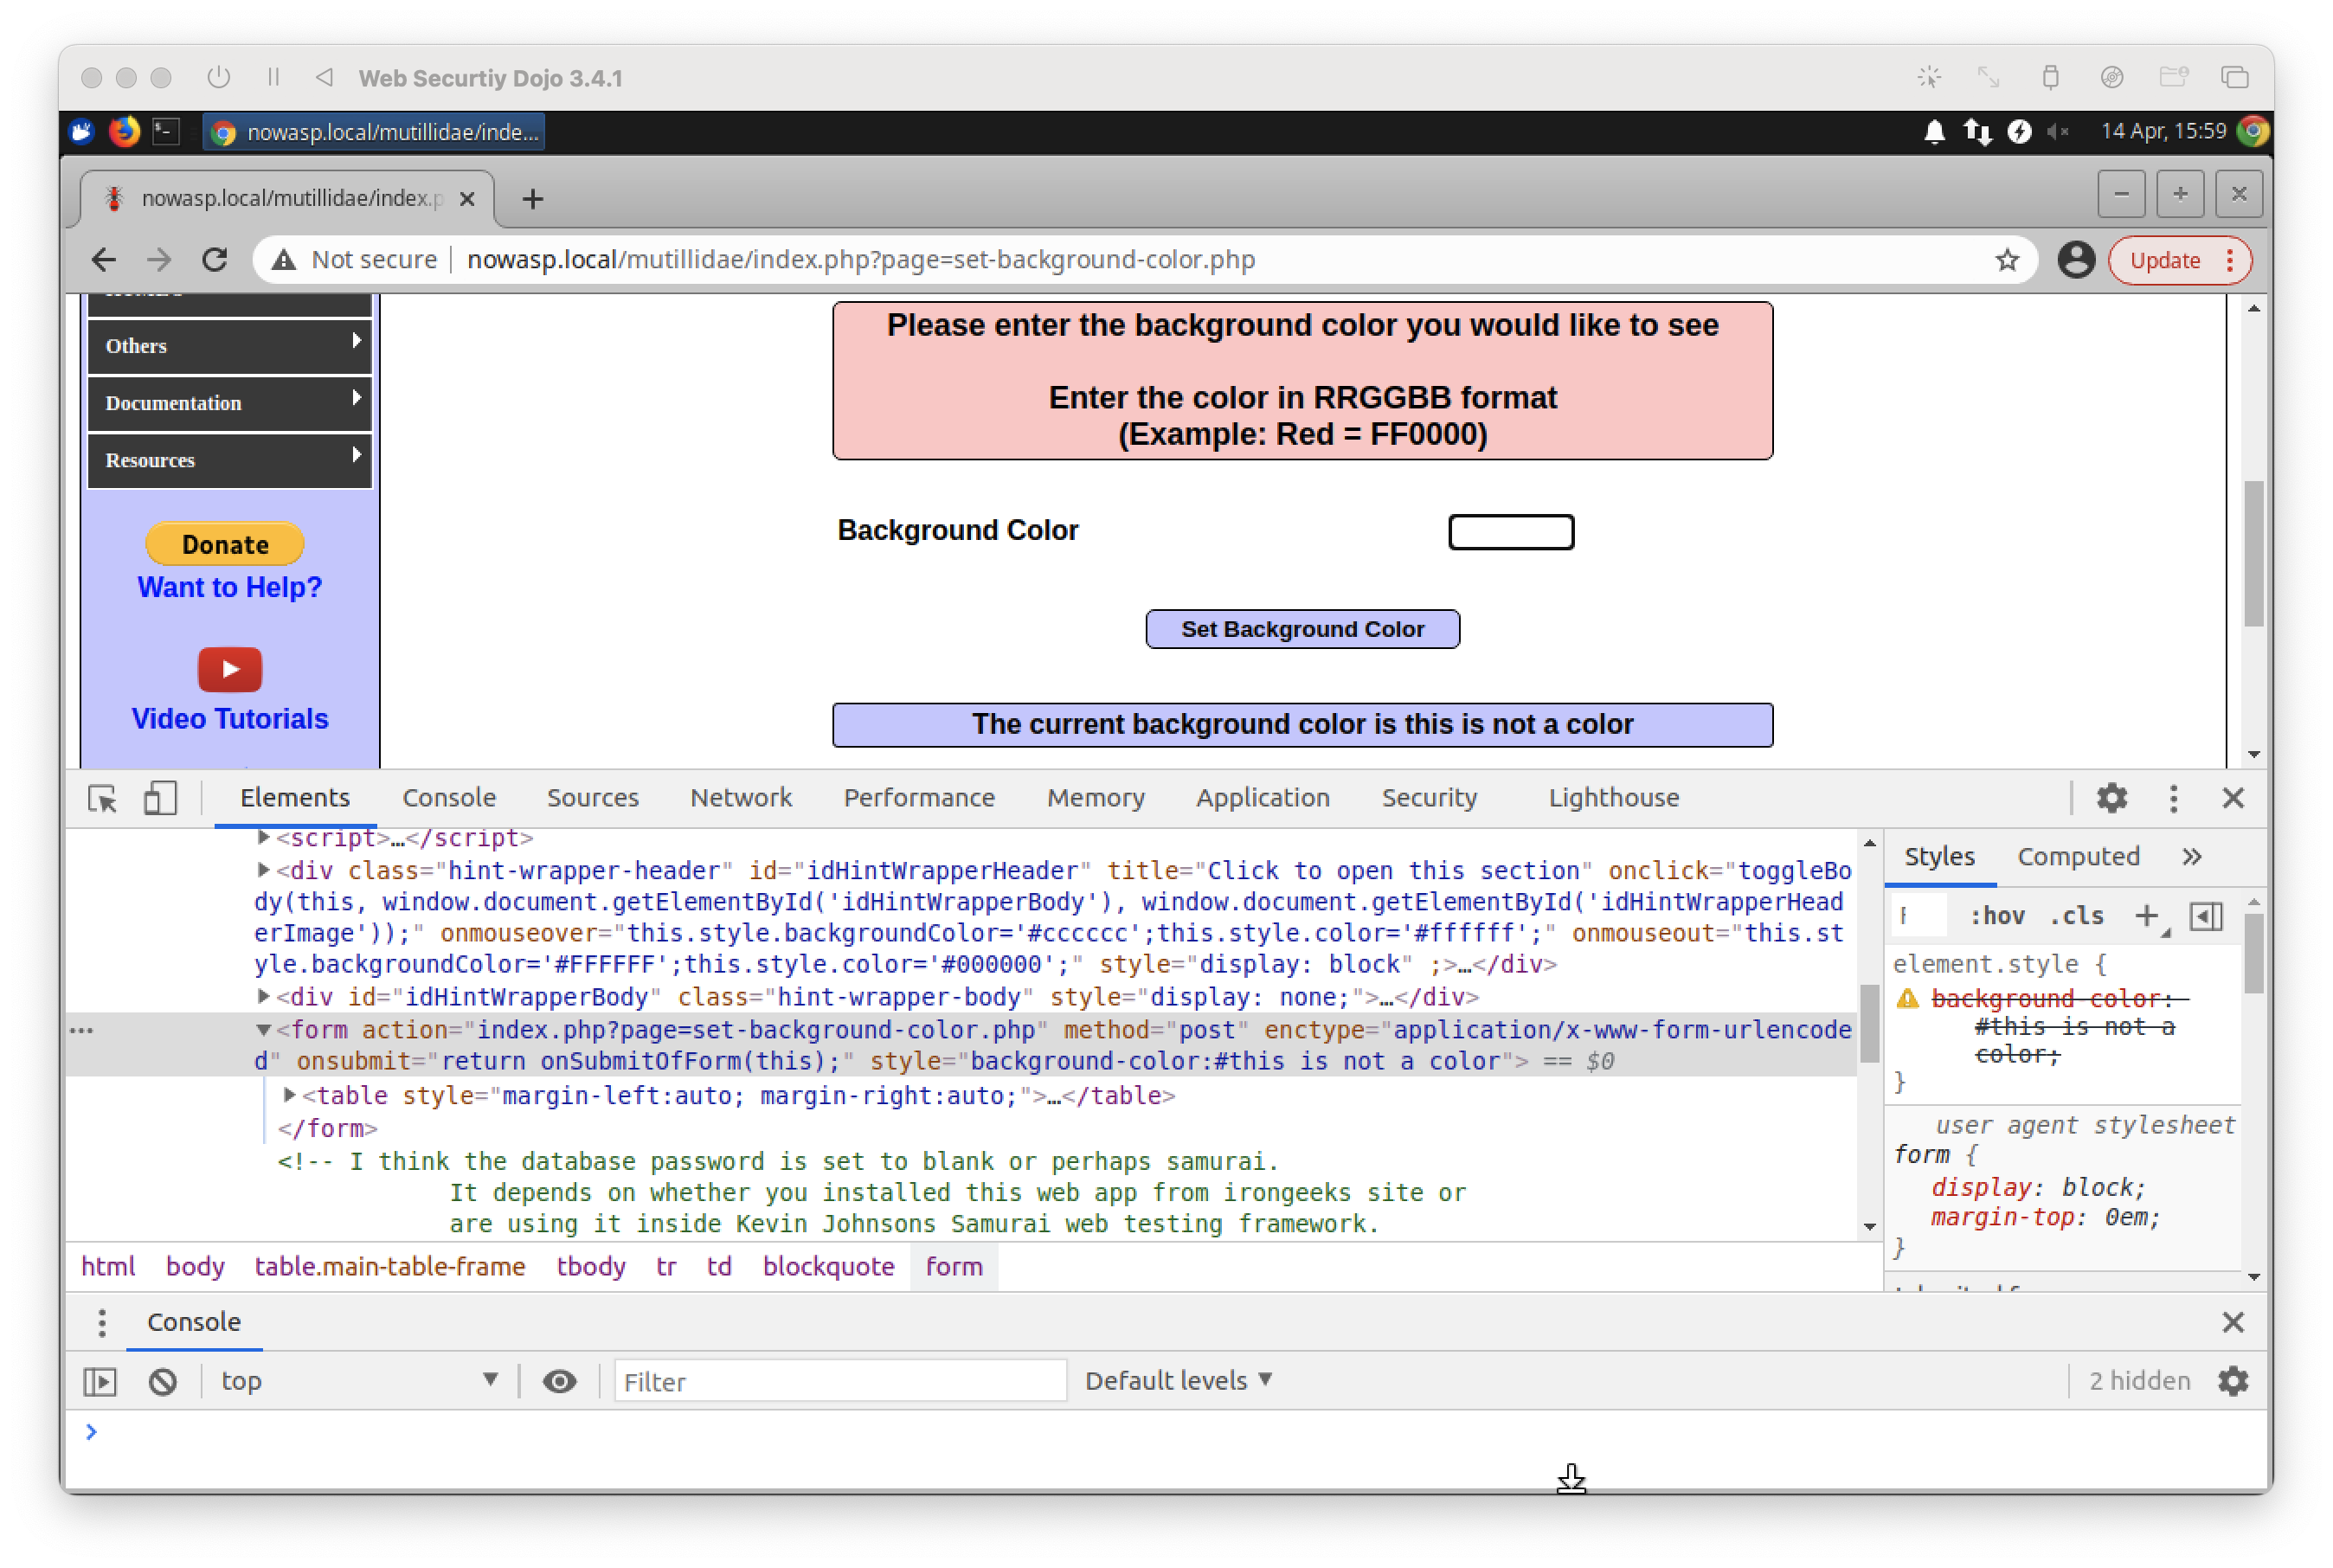
\includegraphics[width=0.8\textwidth]{step_00009}
    \caption{В коде страницы видим, что значение подставилось as is}
  \end{figure}

  Это означает, что в такое поле для ввода мы потенциально можем встроить вредоносный код
  и при установке цвета он отработает. В частности, можно ввести валидный цвет, закрыть
  кавычку, чтобы выйти из редактирования атрибу-та style, и, наконец, закрыть треугольную
  кавычку, чтобы получить возможность вставлять свой собственный html код:

  \begin{figure}[H]
    \centering
    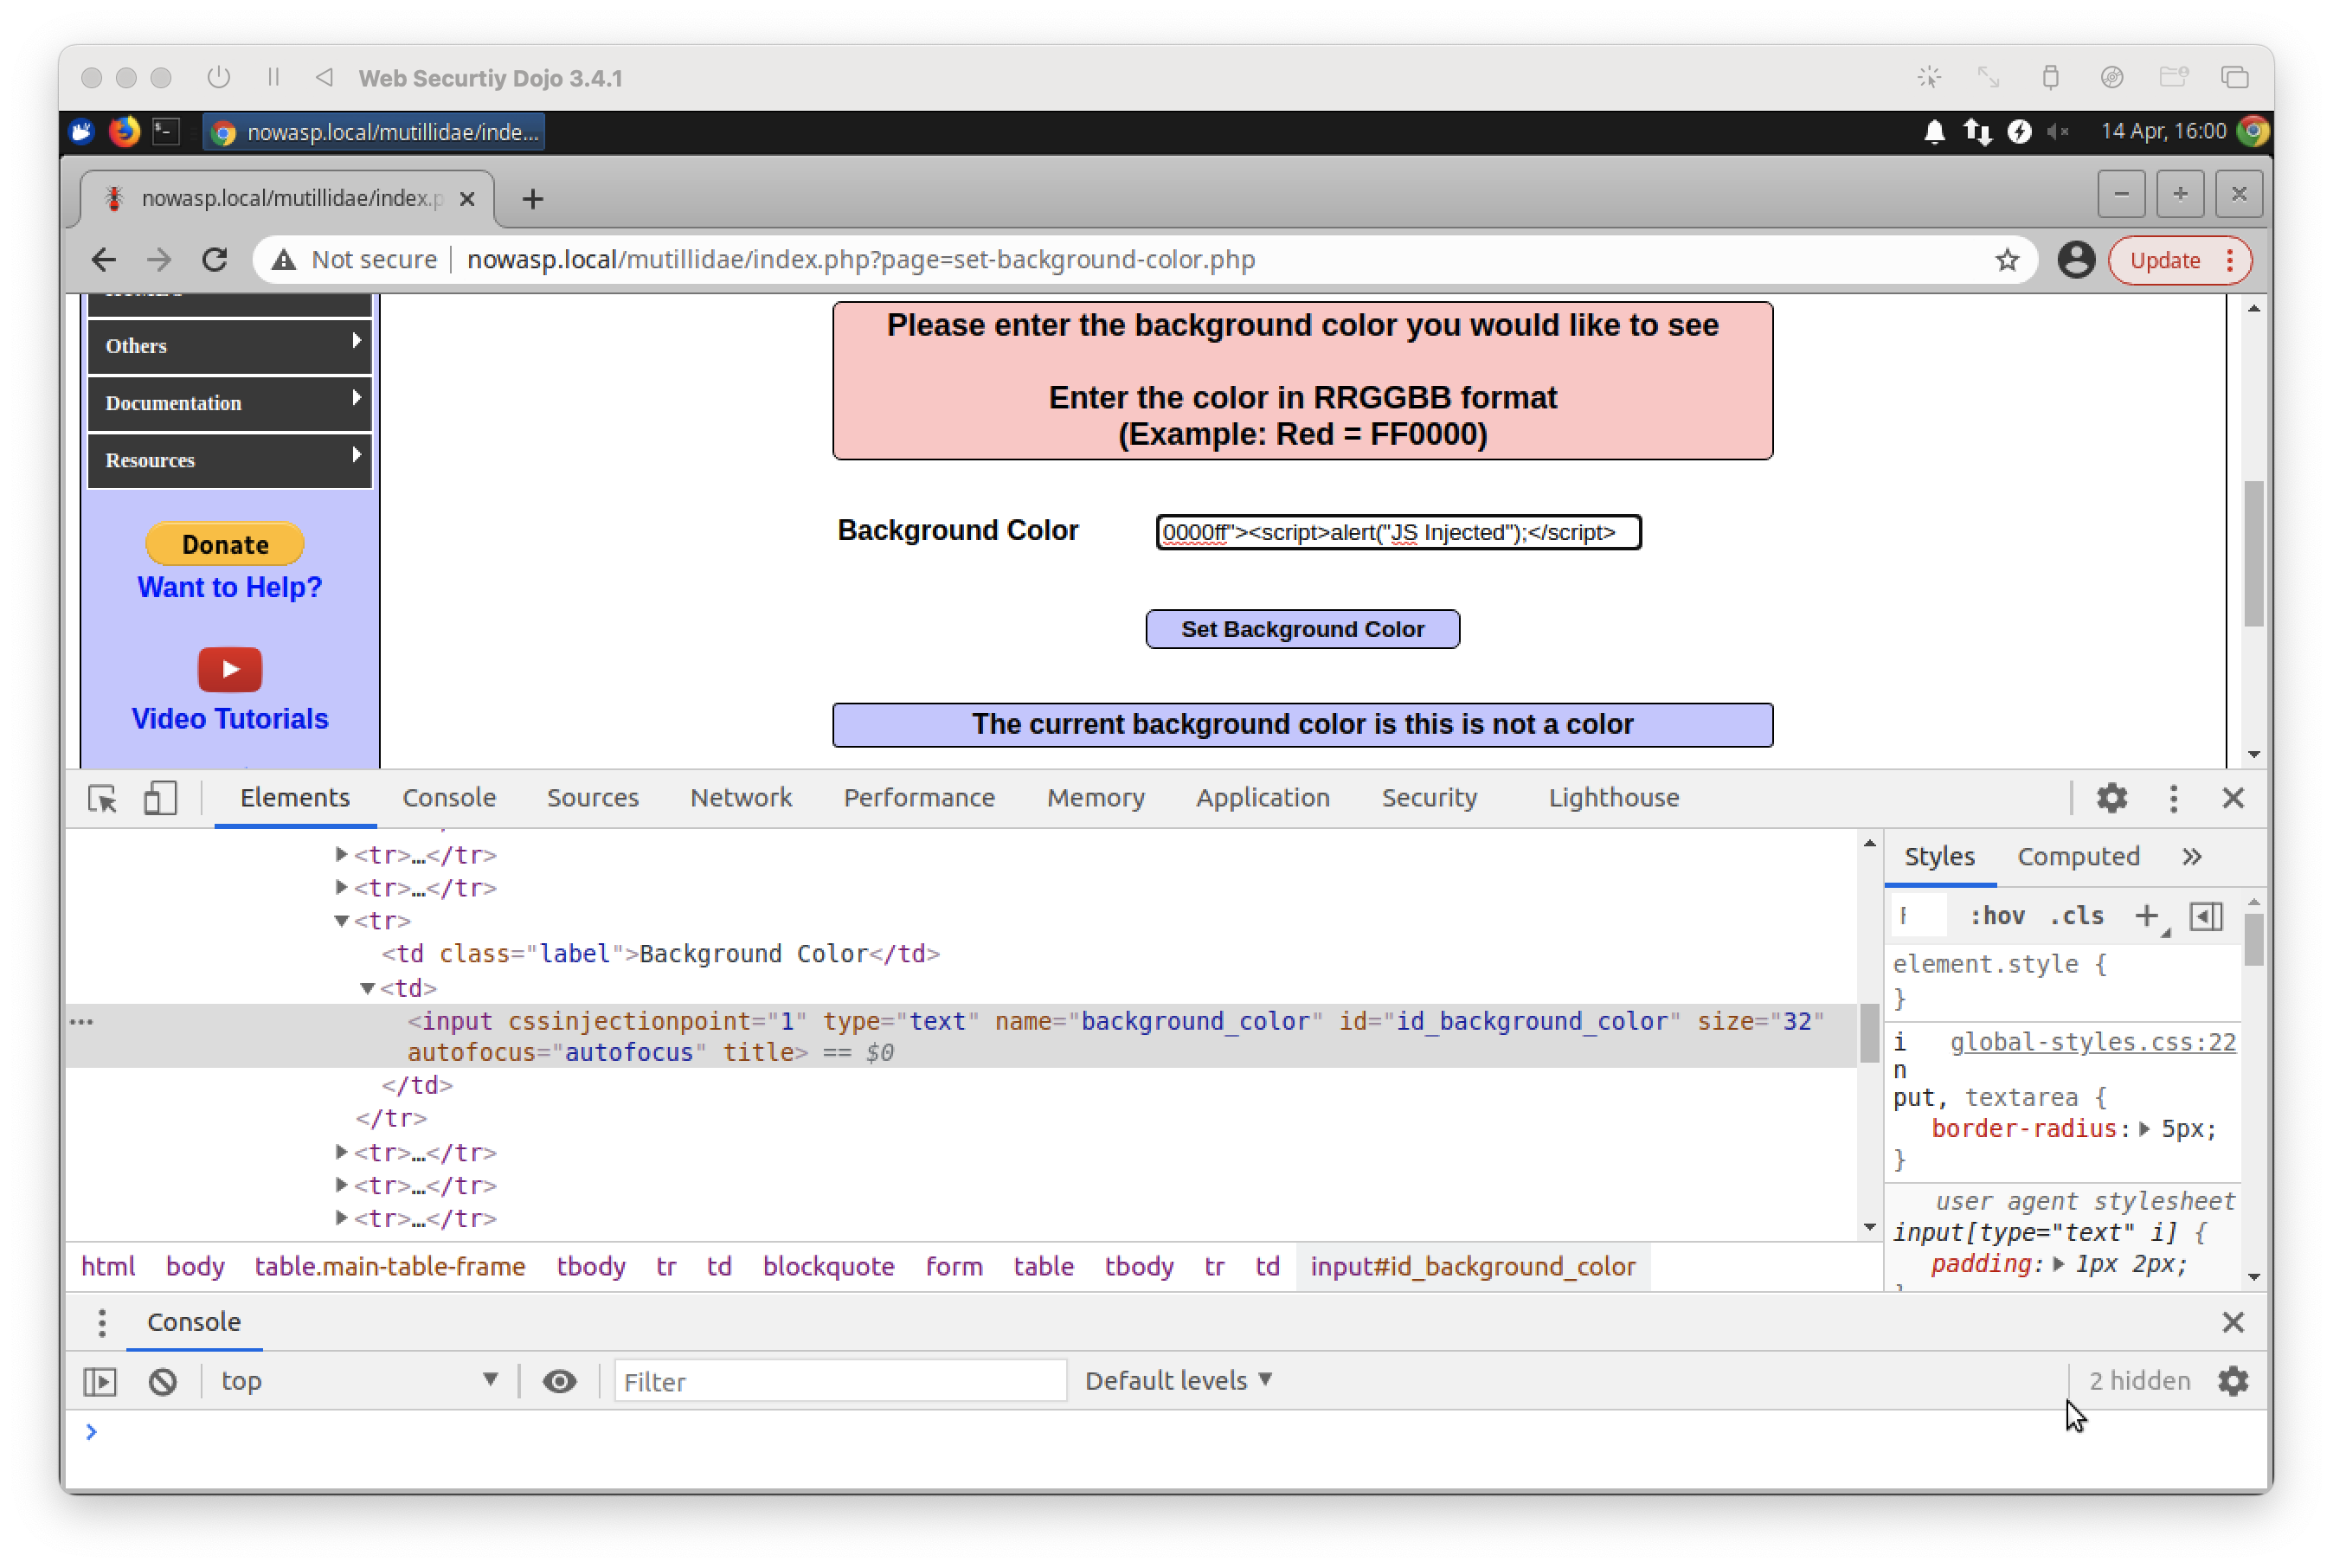
\includegraphics[width=0.8\textwidth]{step_00010}
    \caption{Закрыли все теги и вставили собственный script тег с вызовом сообщения о взломе}
  \end{figure}

  \begin{figure}[H]
    \centering
    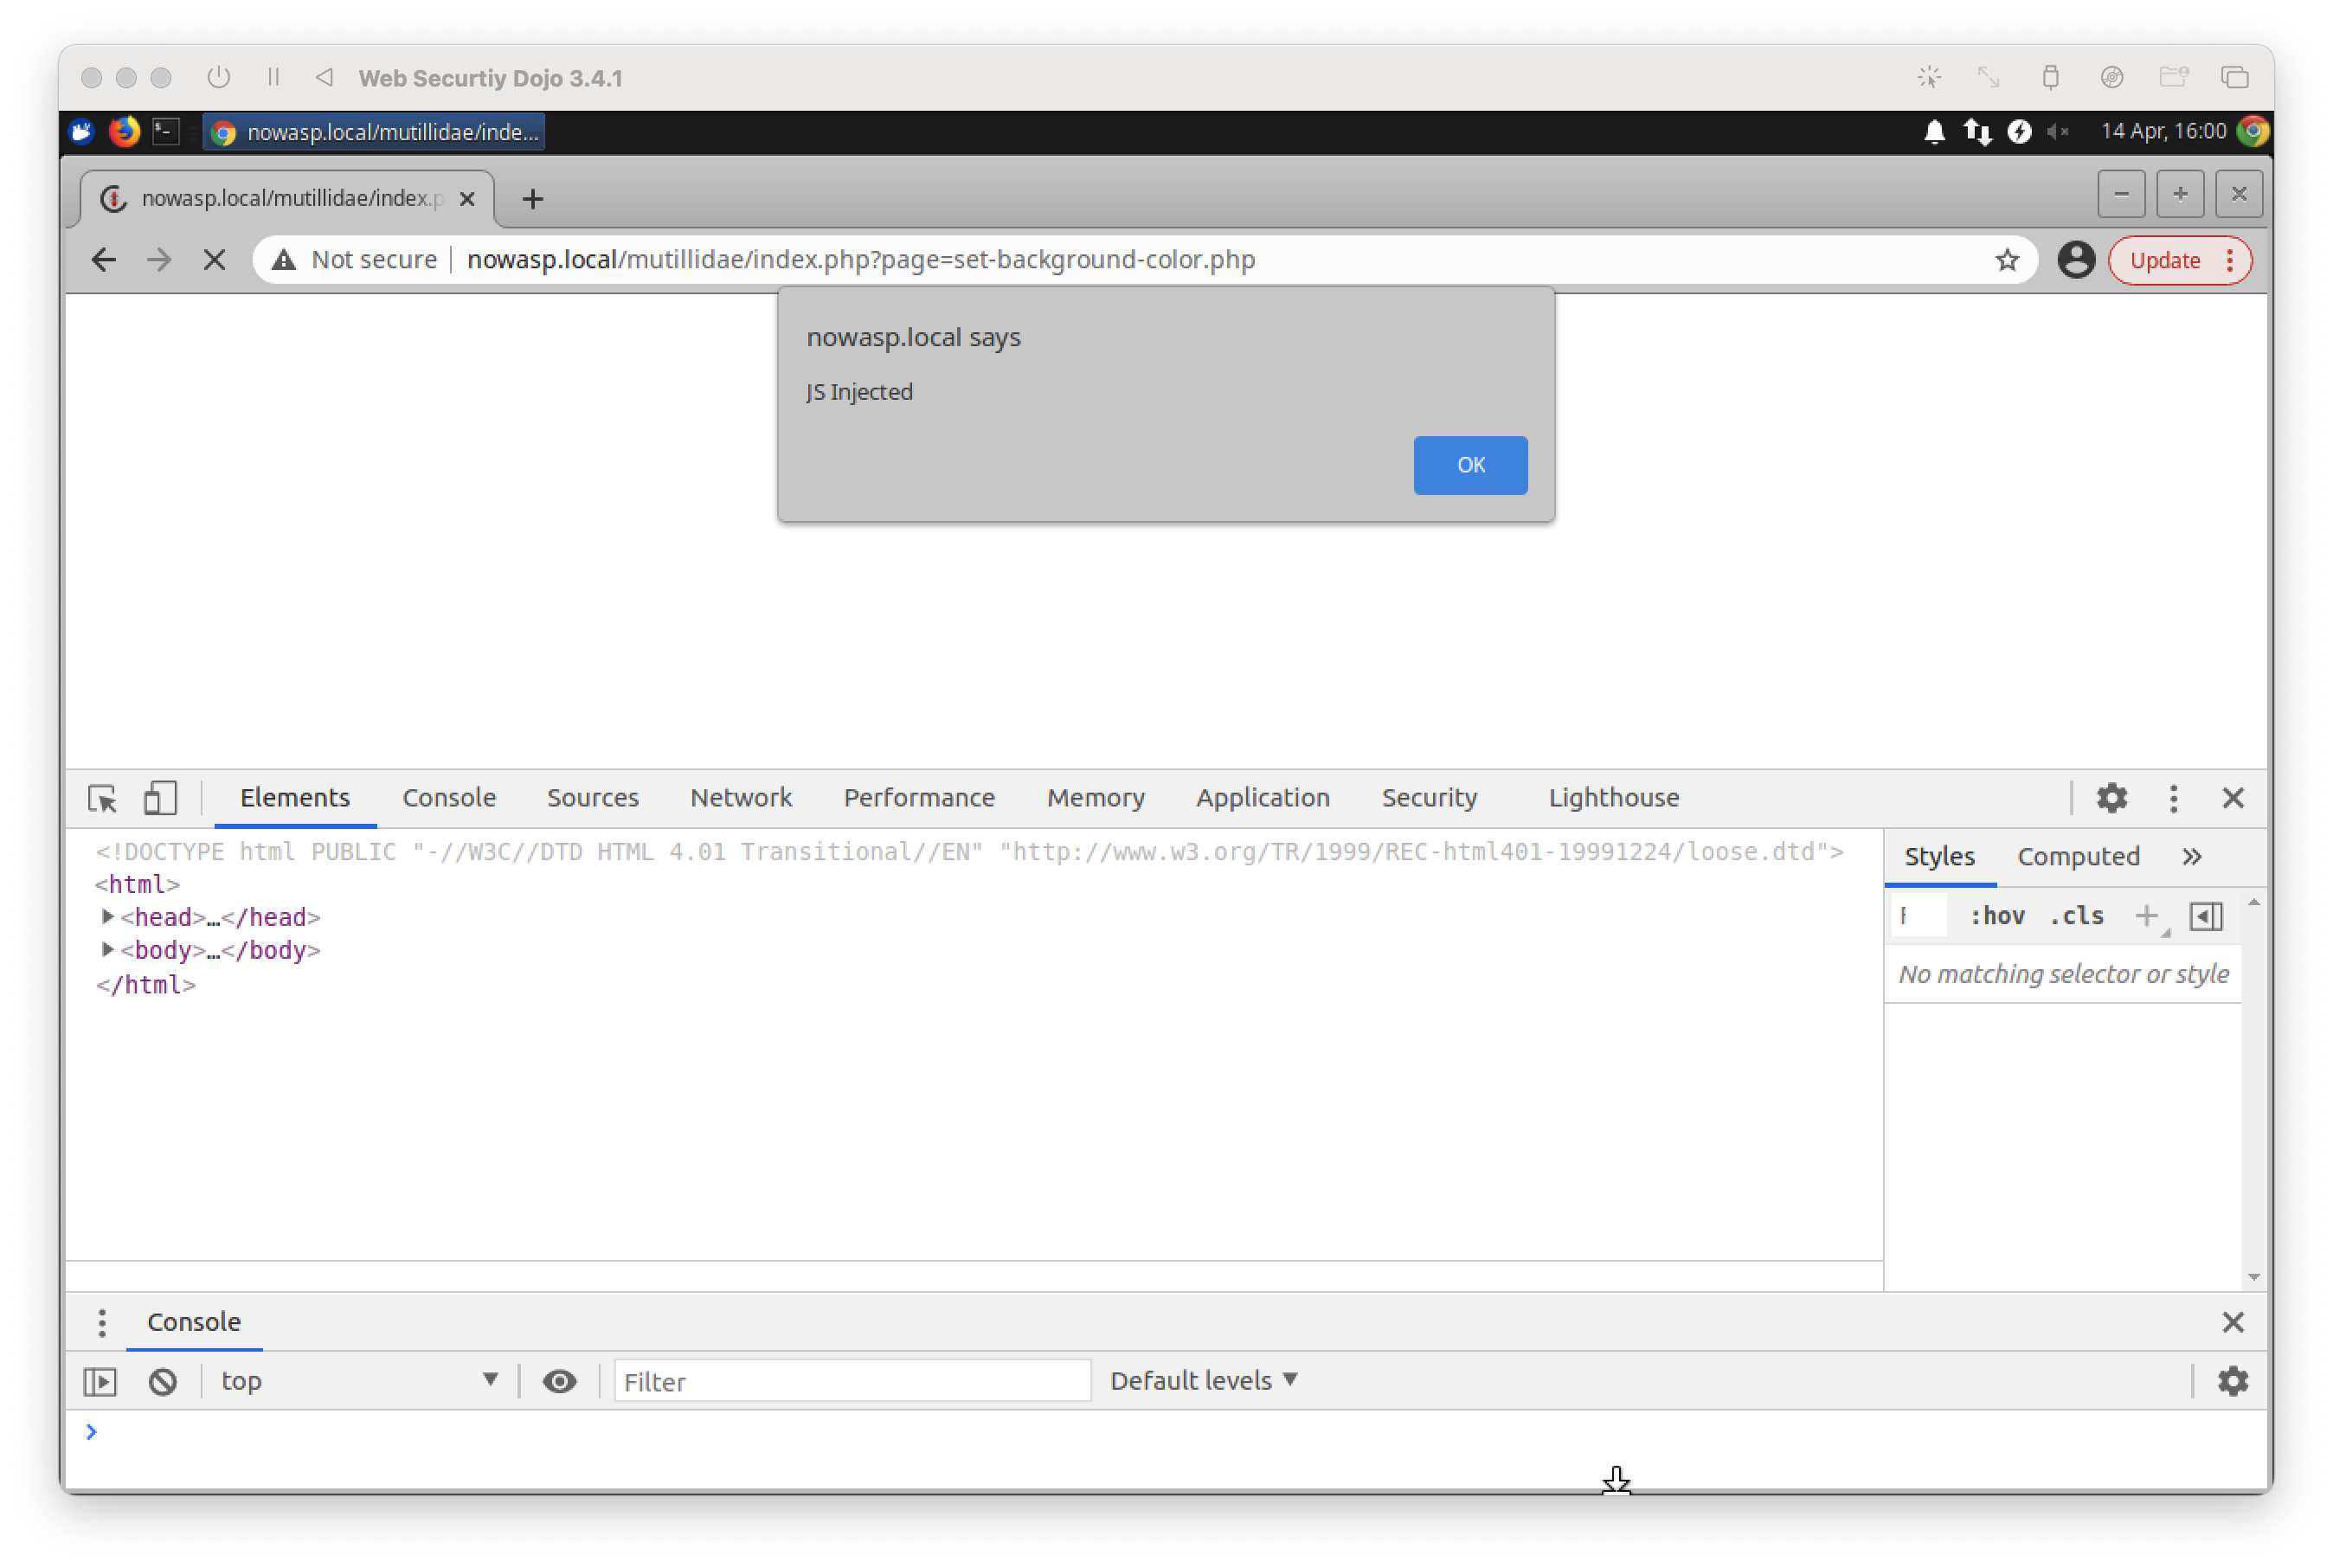
\includegraphics[width=0.8\textwidth]{step_00011}
    \caption{Нажатие на кнопку привело к ожидаемому результату}
  \end{figure}

  \begin{figure}[H]
    \centering
    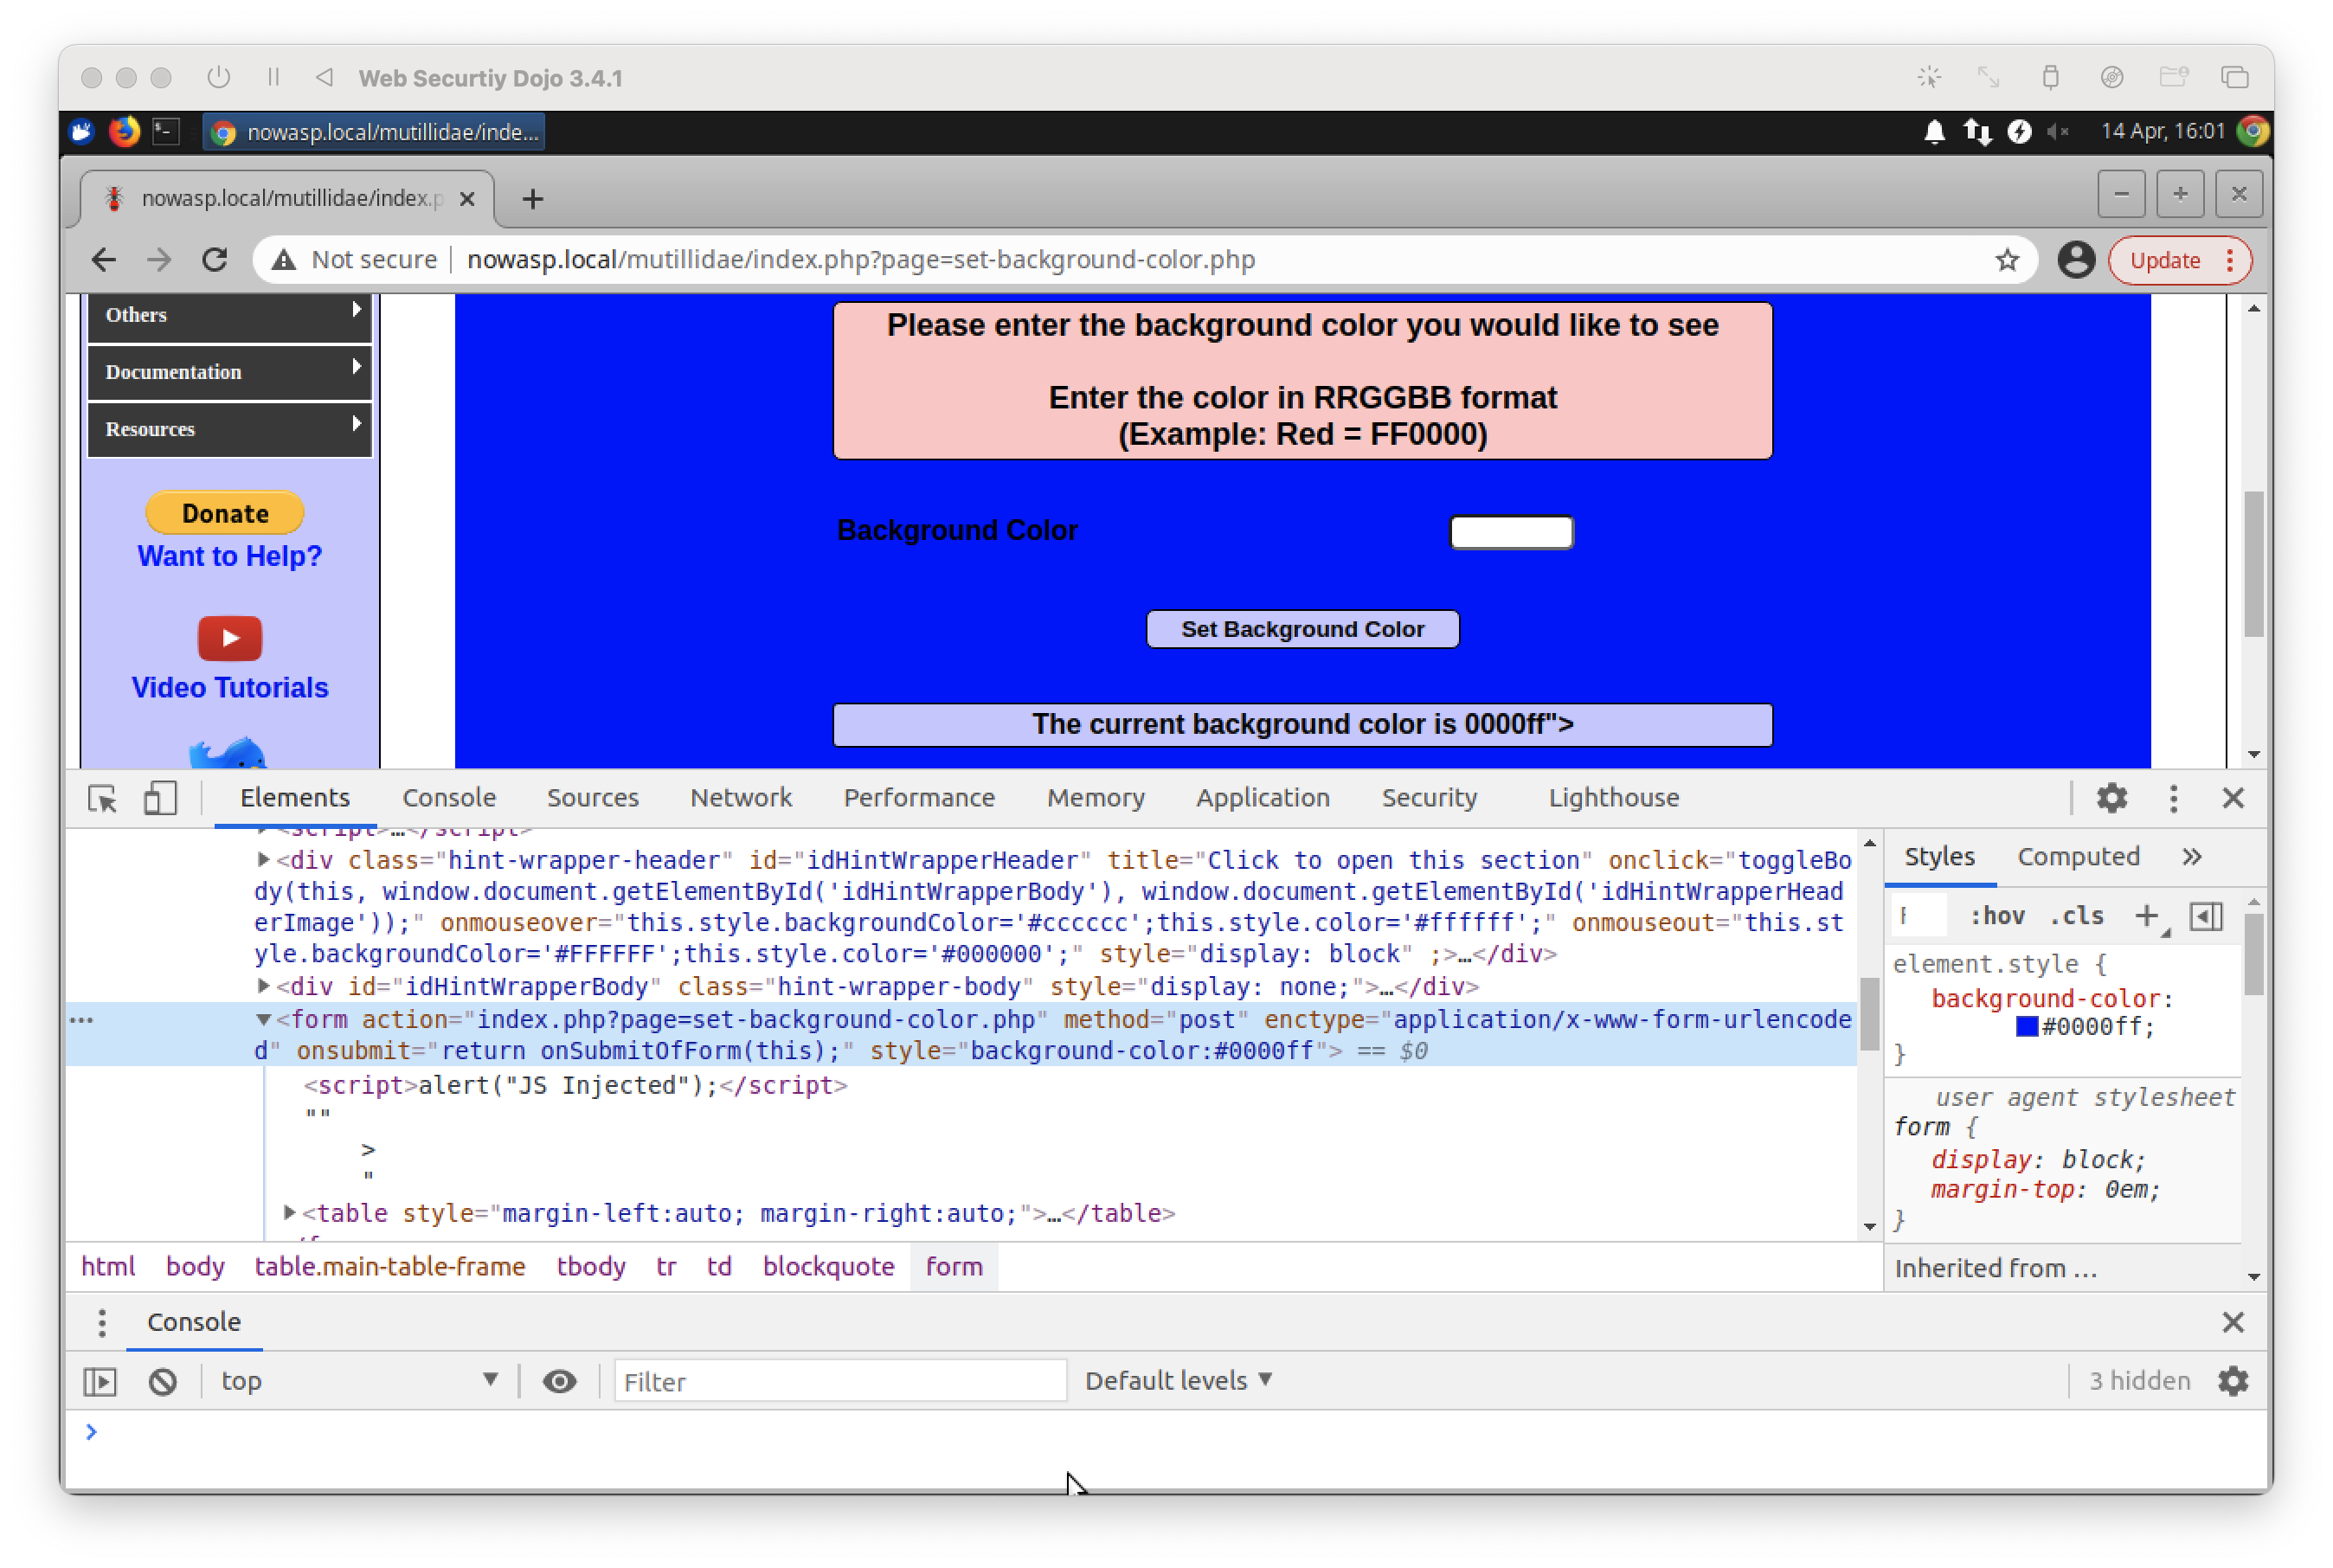
\includegraphics[width=0.8\textwidth]{step_00012}
    \caption{При рассмотрении html разметки видим наш script тег}
  \end{figure}

  Теперь попробуем вставить полноценный, незаметный для пользователя ajax запрос,
  ворующий все Cookie ресурса:

  \begin{figure}[H]
    \centering
    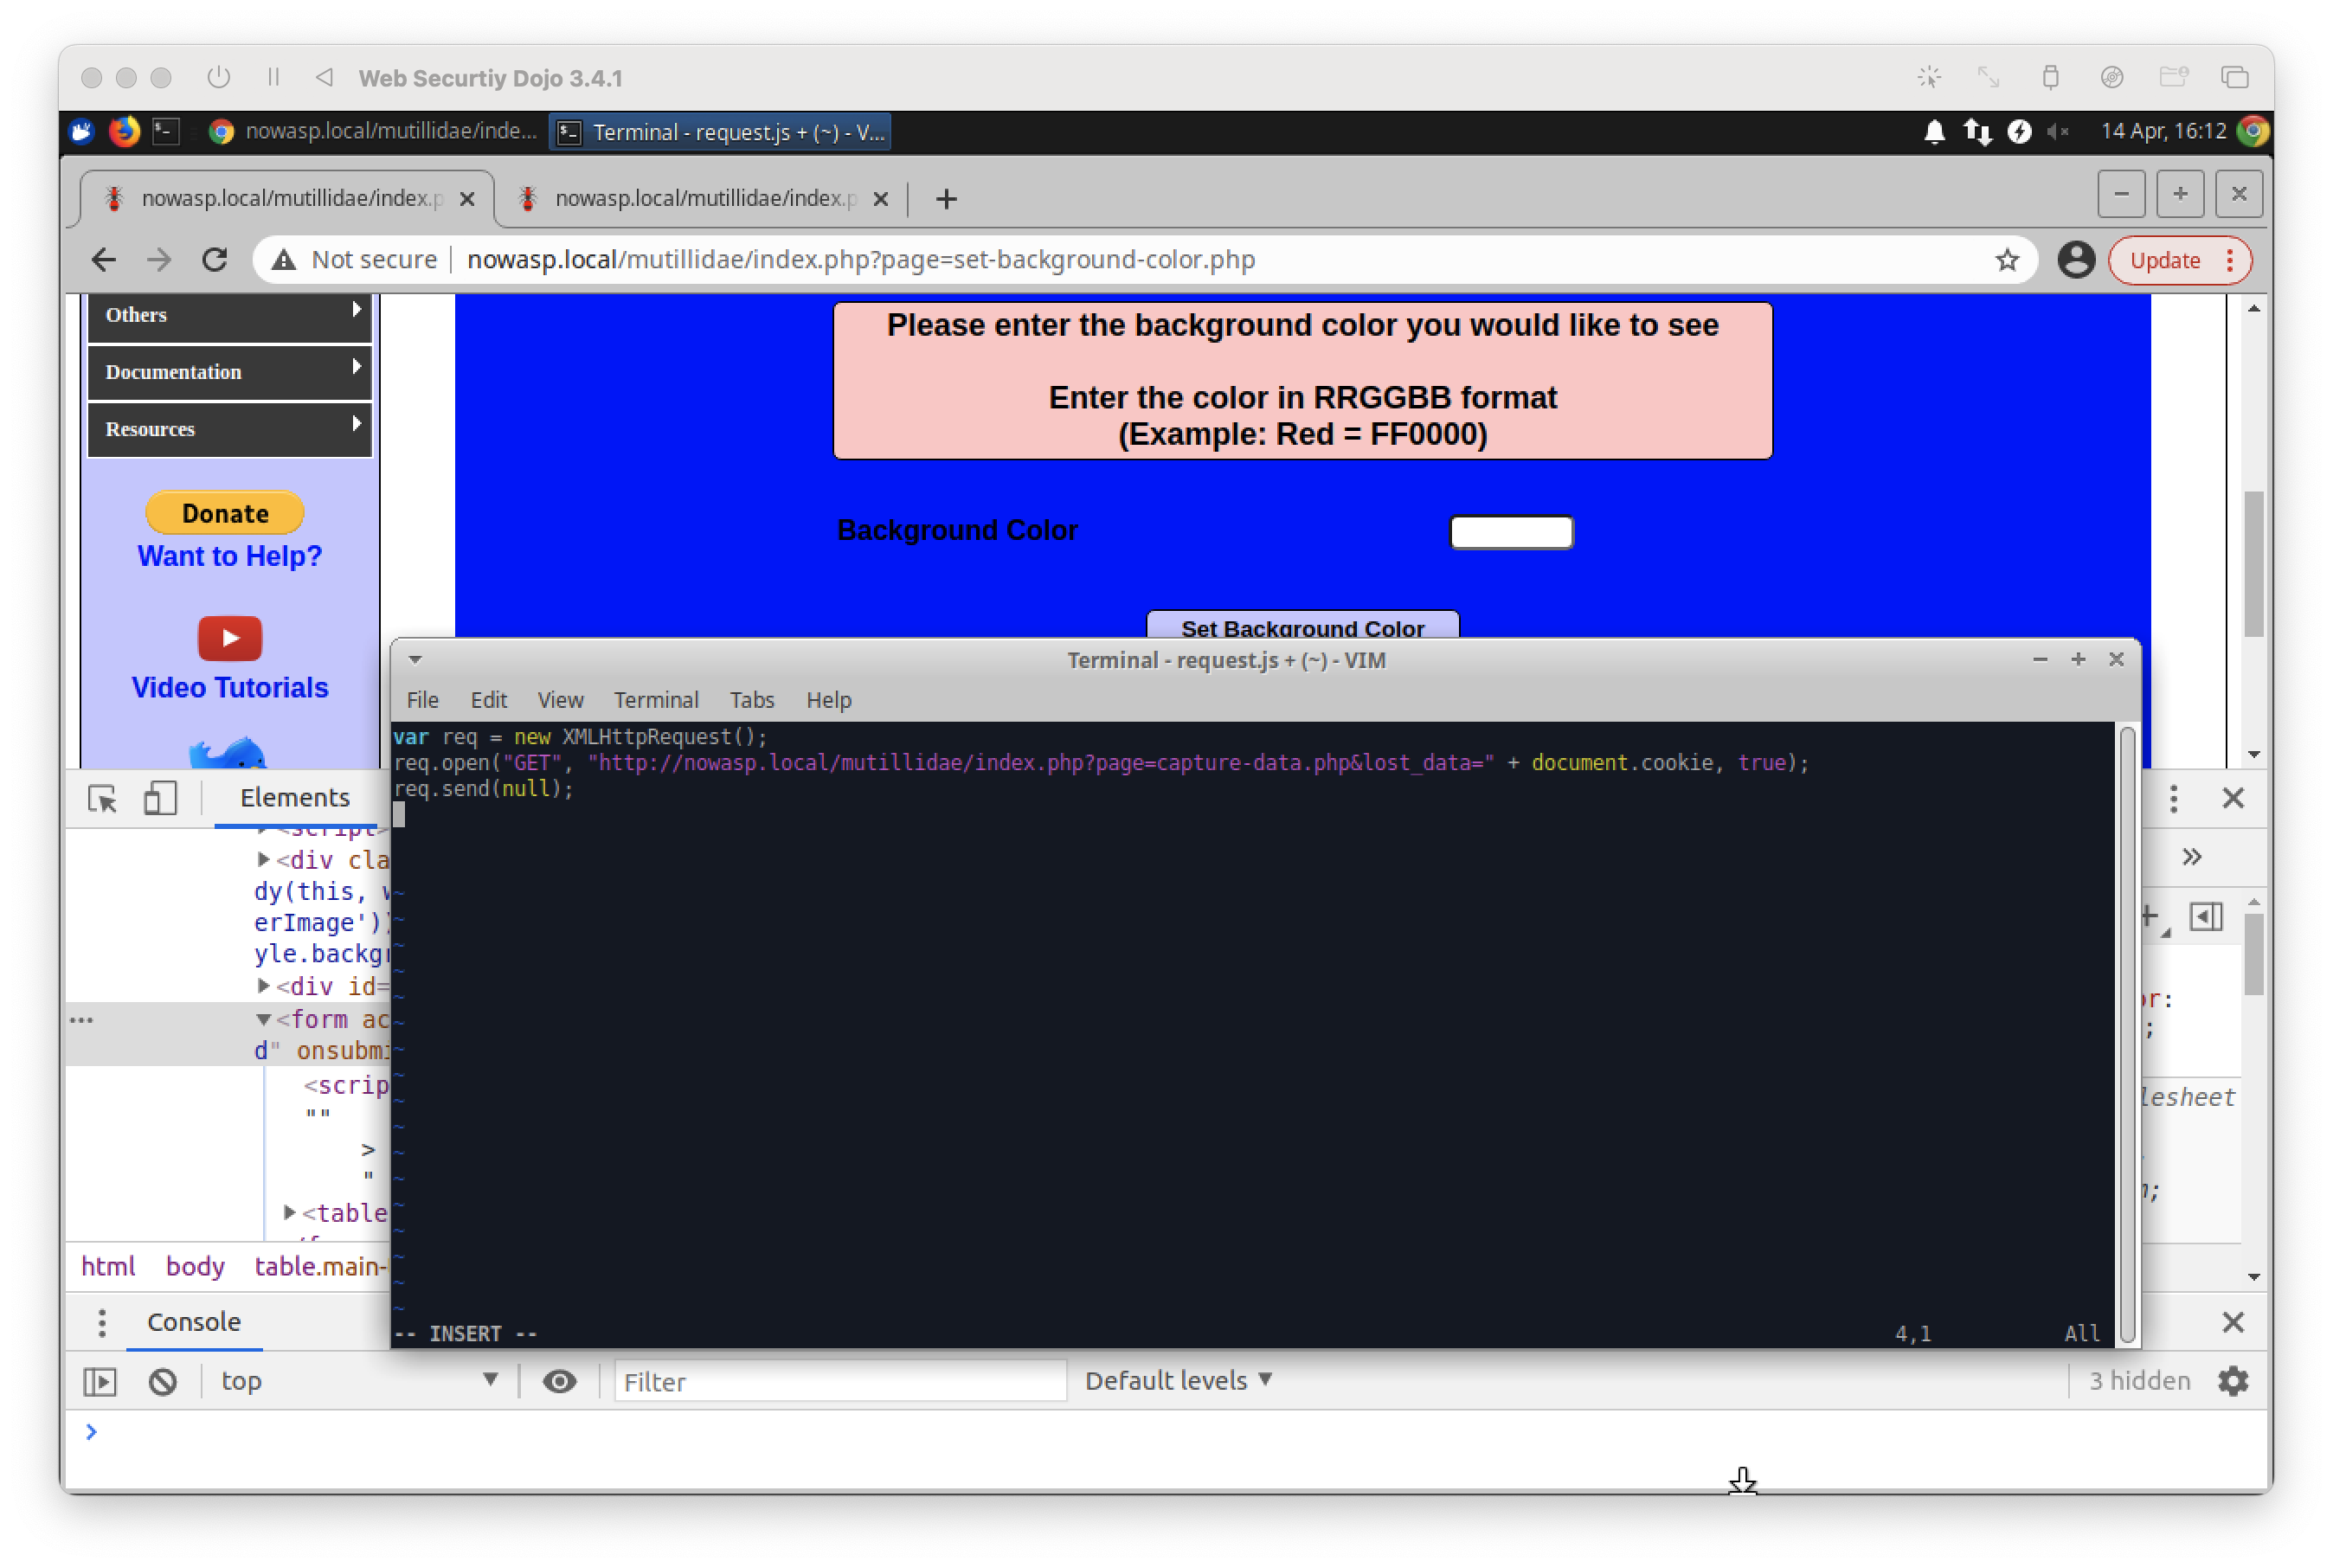
\includegraphics[width=0.8\textwidth]{step_00016}
    \caption{Код запроса на JS}
  \end{figure}

  \begin{figure}[H]
    \centering
    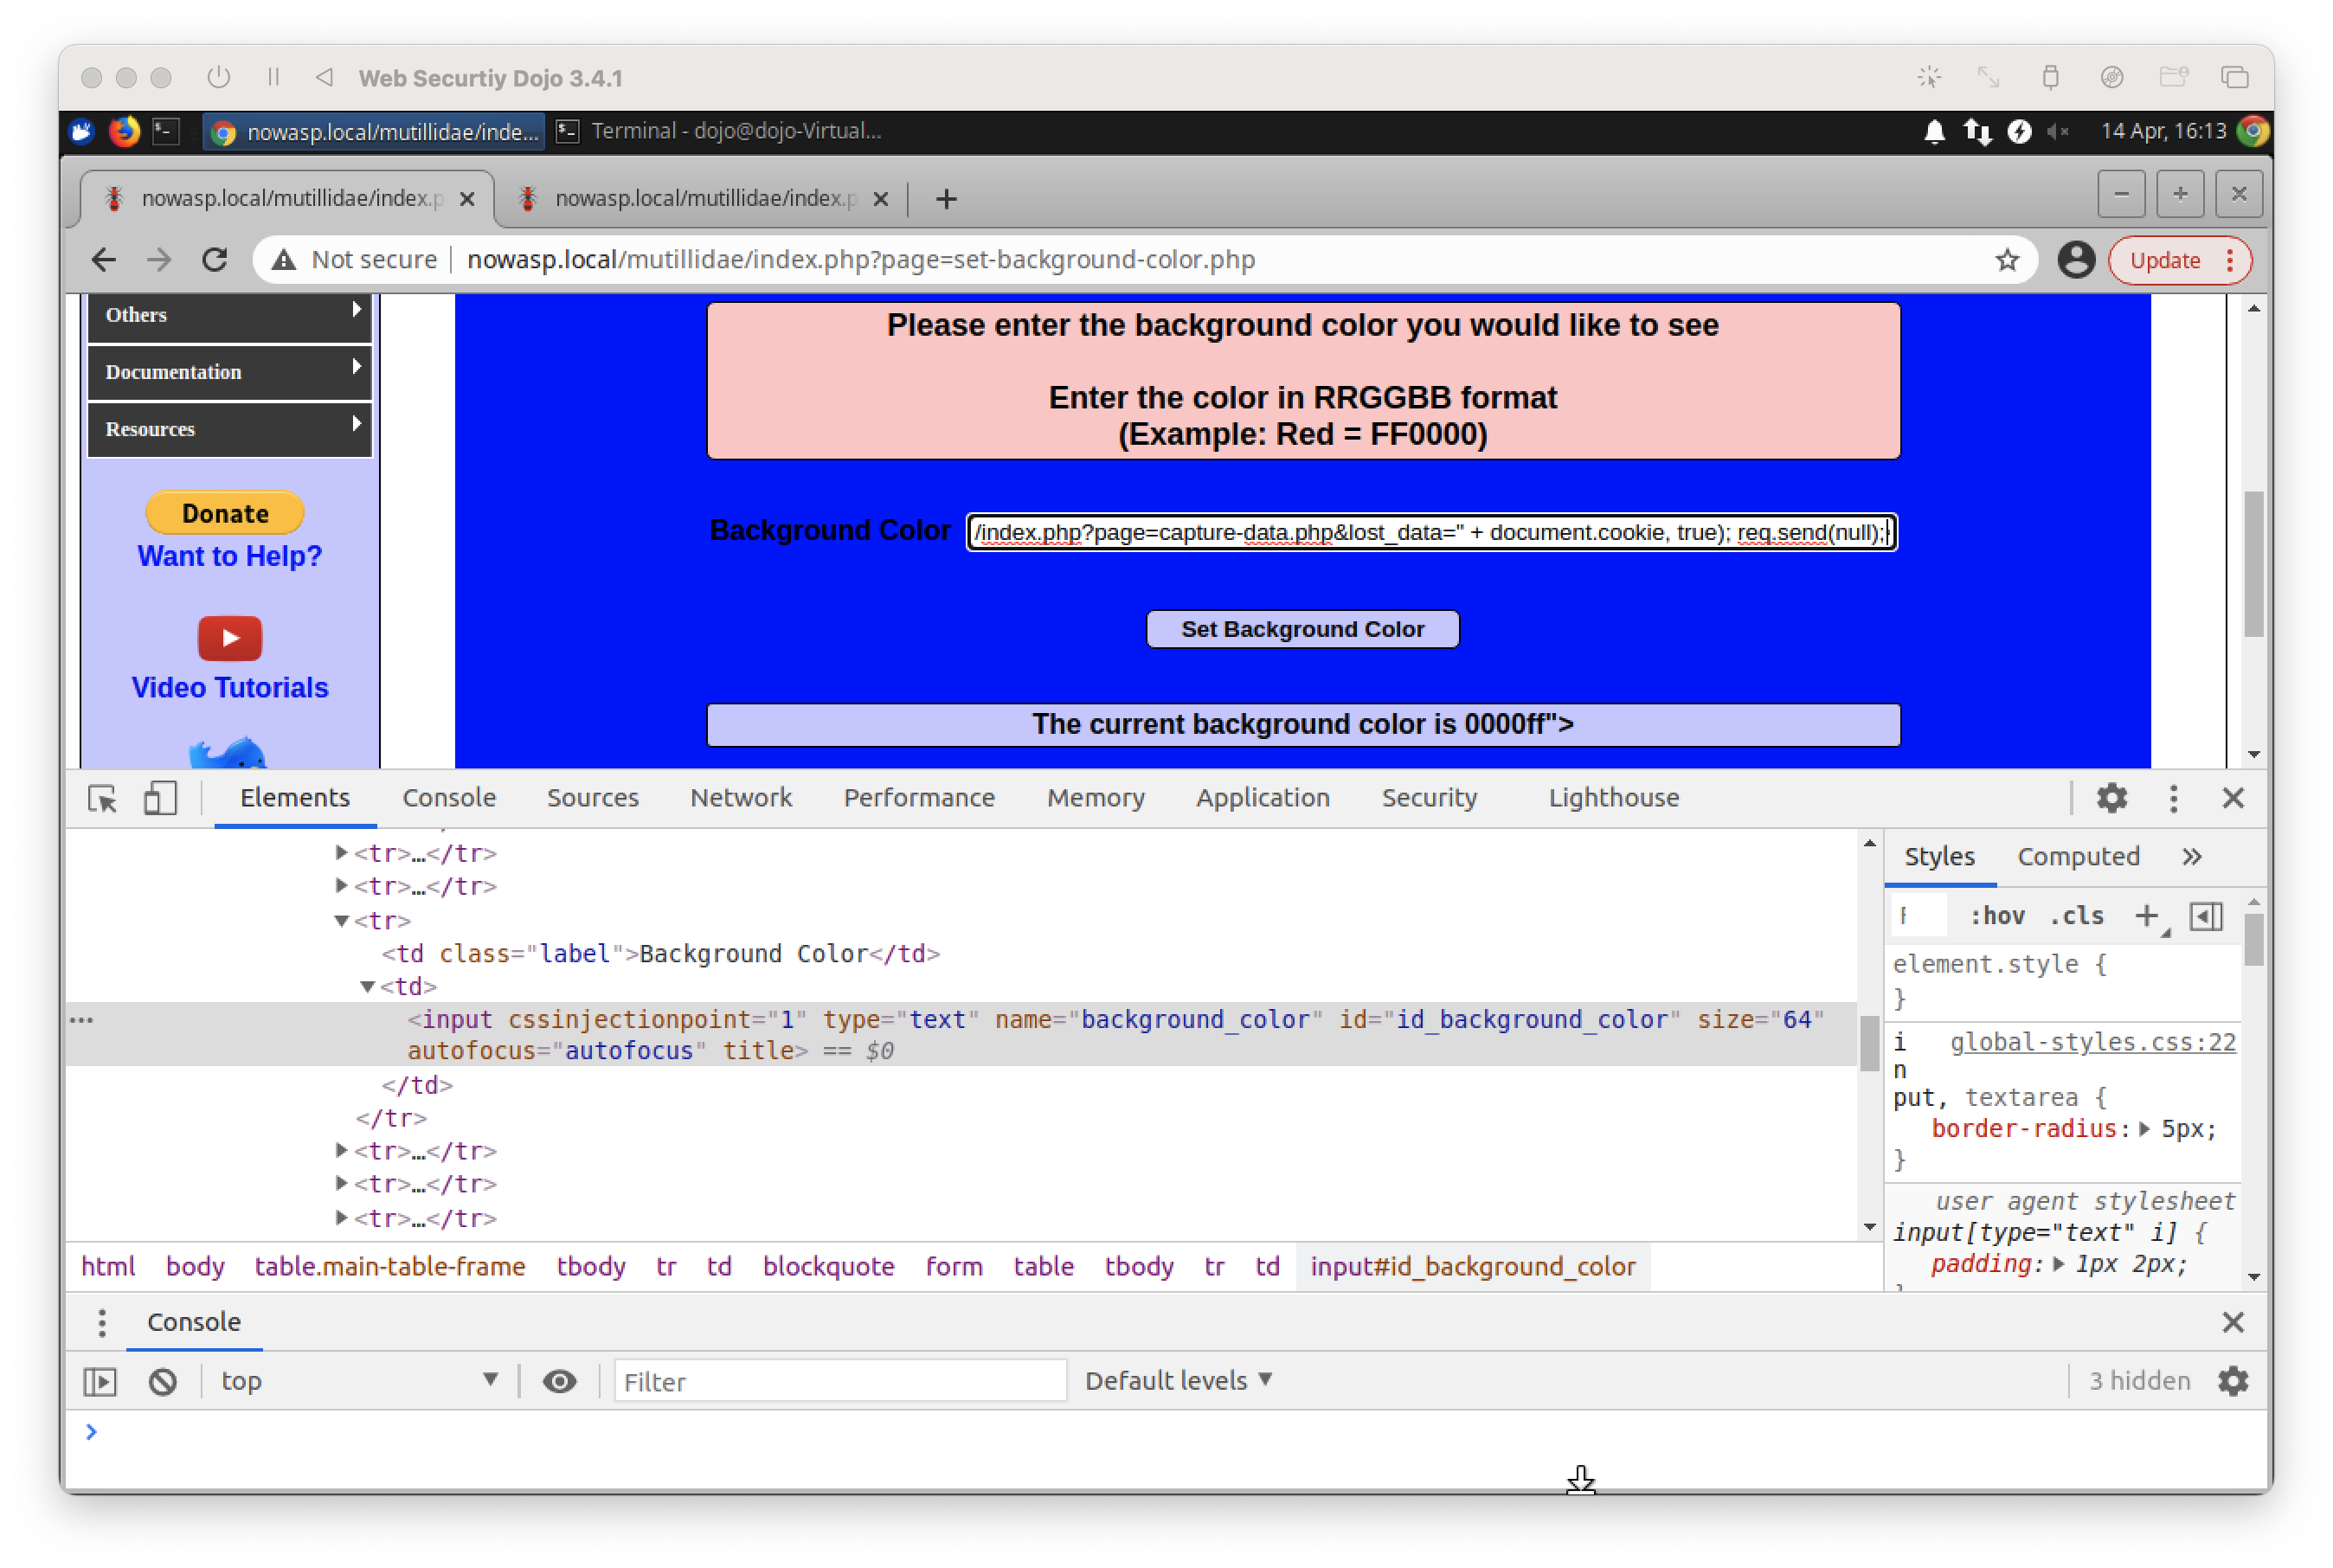
\includegraphics[width=0.8\textwidth]{step_00017}
    \caption{Встаиваем код в объект атаки}
  \end{figure}

  \begin{figure}[H]
    \centering
    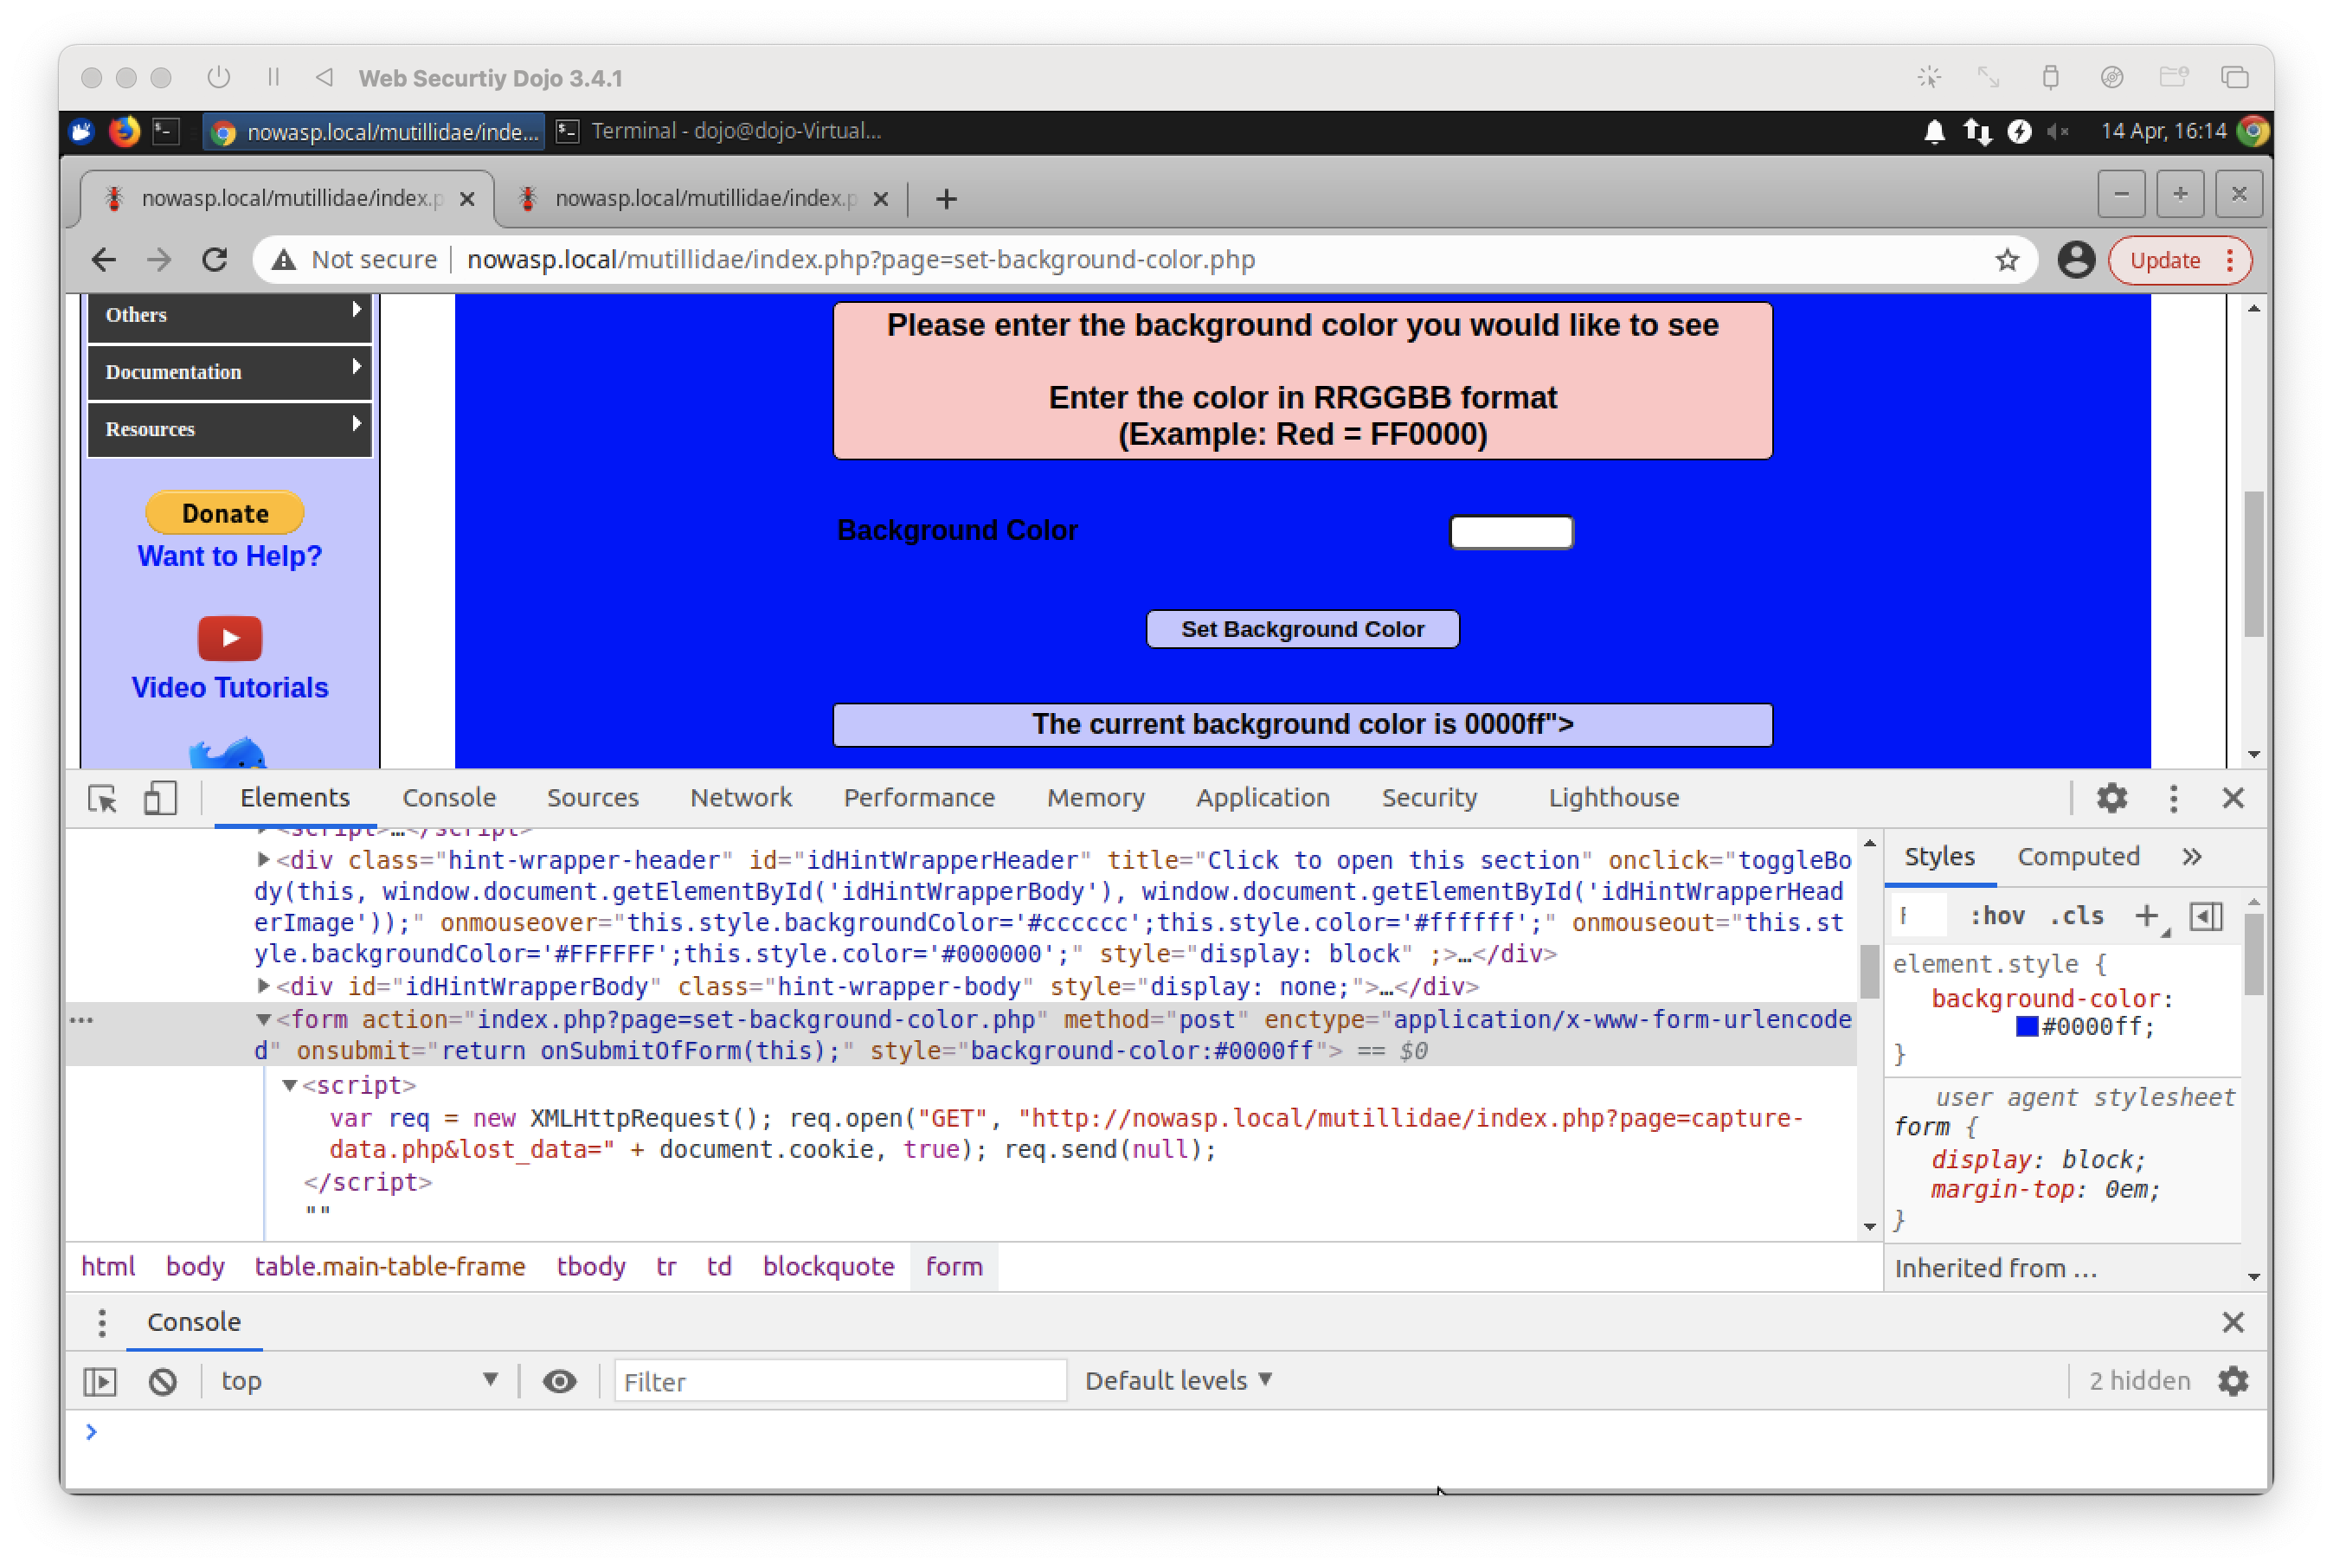
\includegraphics[width=0.8\textwidth]{step_00018}
    \caption{После нажатия кнопки обновления цвета видим в html разметке незаметную отправку Cookie злоумышленнику}
  \end{figure}

  \begin{figure}[H]
    \centering
    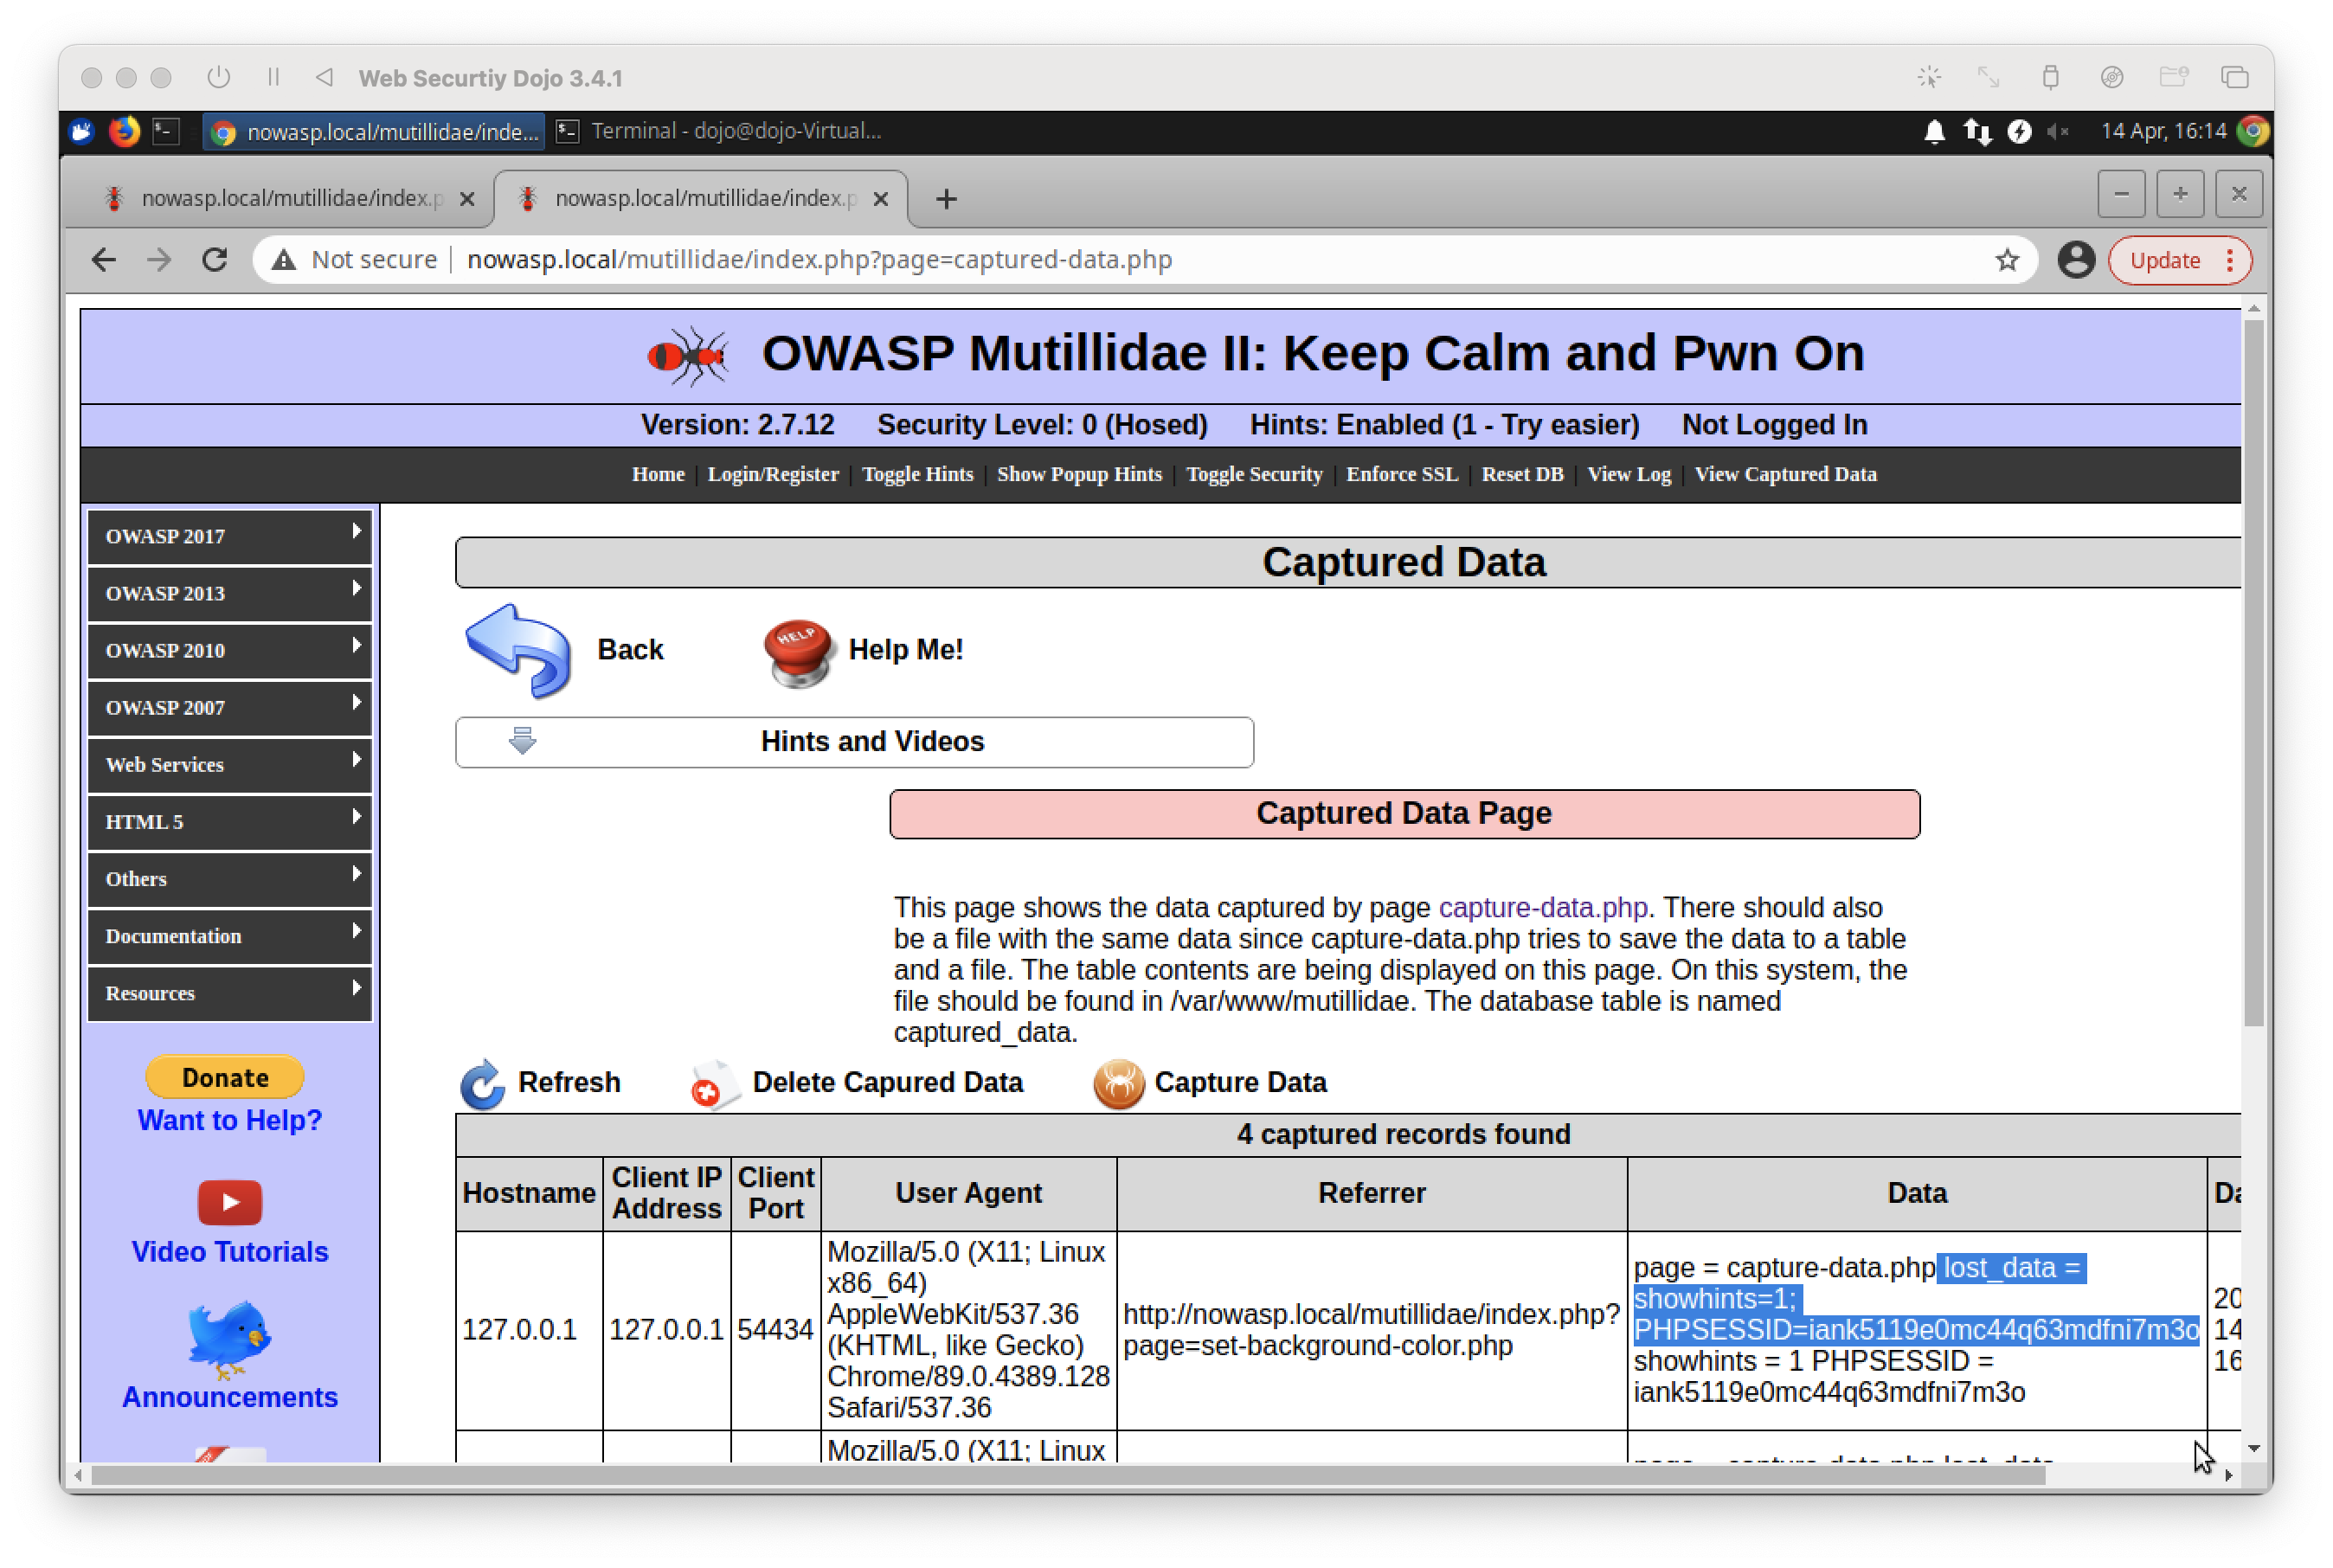
\includegraphics[width=0.8\textwidth]{step_00019}
    \caption{По истории видим, что сессия действительно была украдена}
  \end{figure}

  \subsection{Атака Data Capture Page}

  Эту страницу мы используем для обработки украденных Cookie, но мо-жет и она
  обладает некими уязвимостями. Попробуем узнать, может ли хакер быть взломан
  другим хакером:

  \begin{figure}[H]
    \centering
    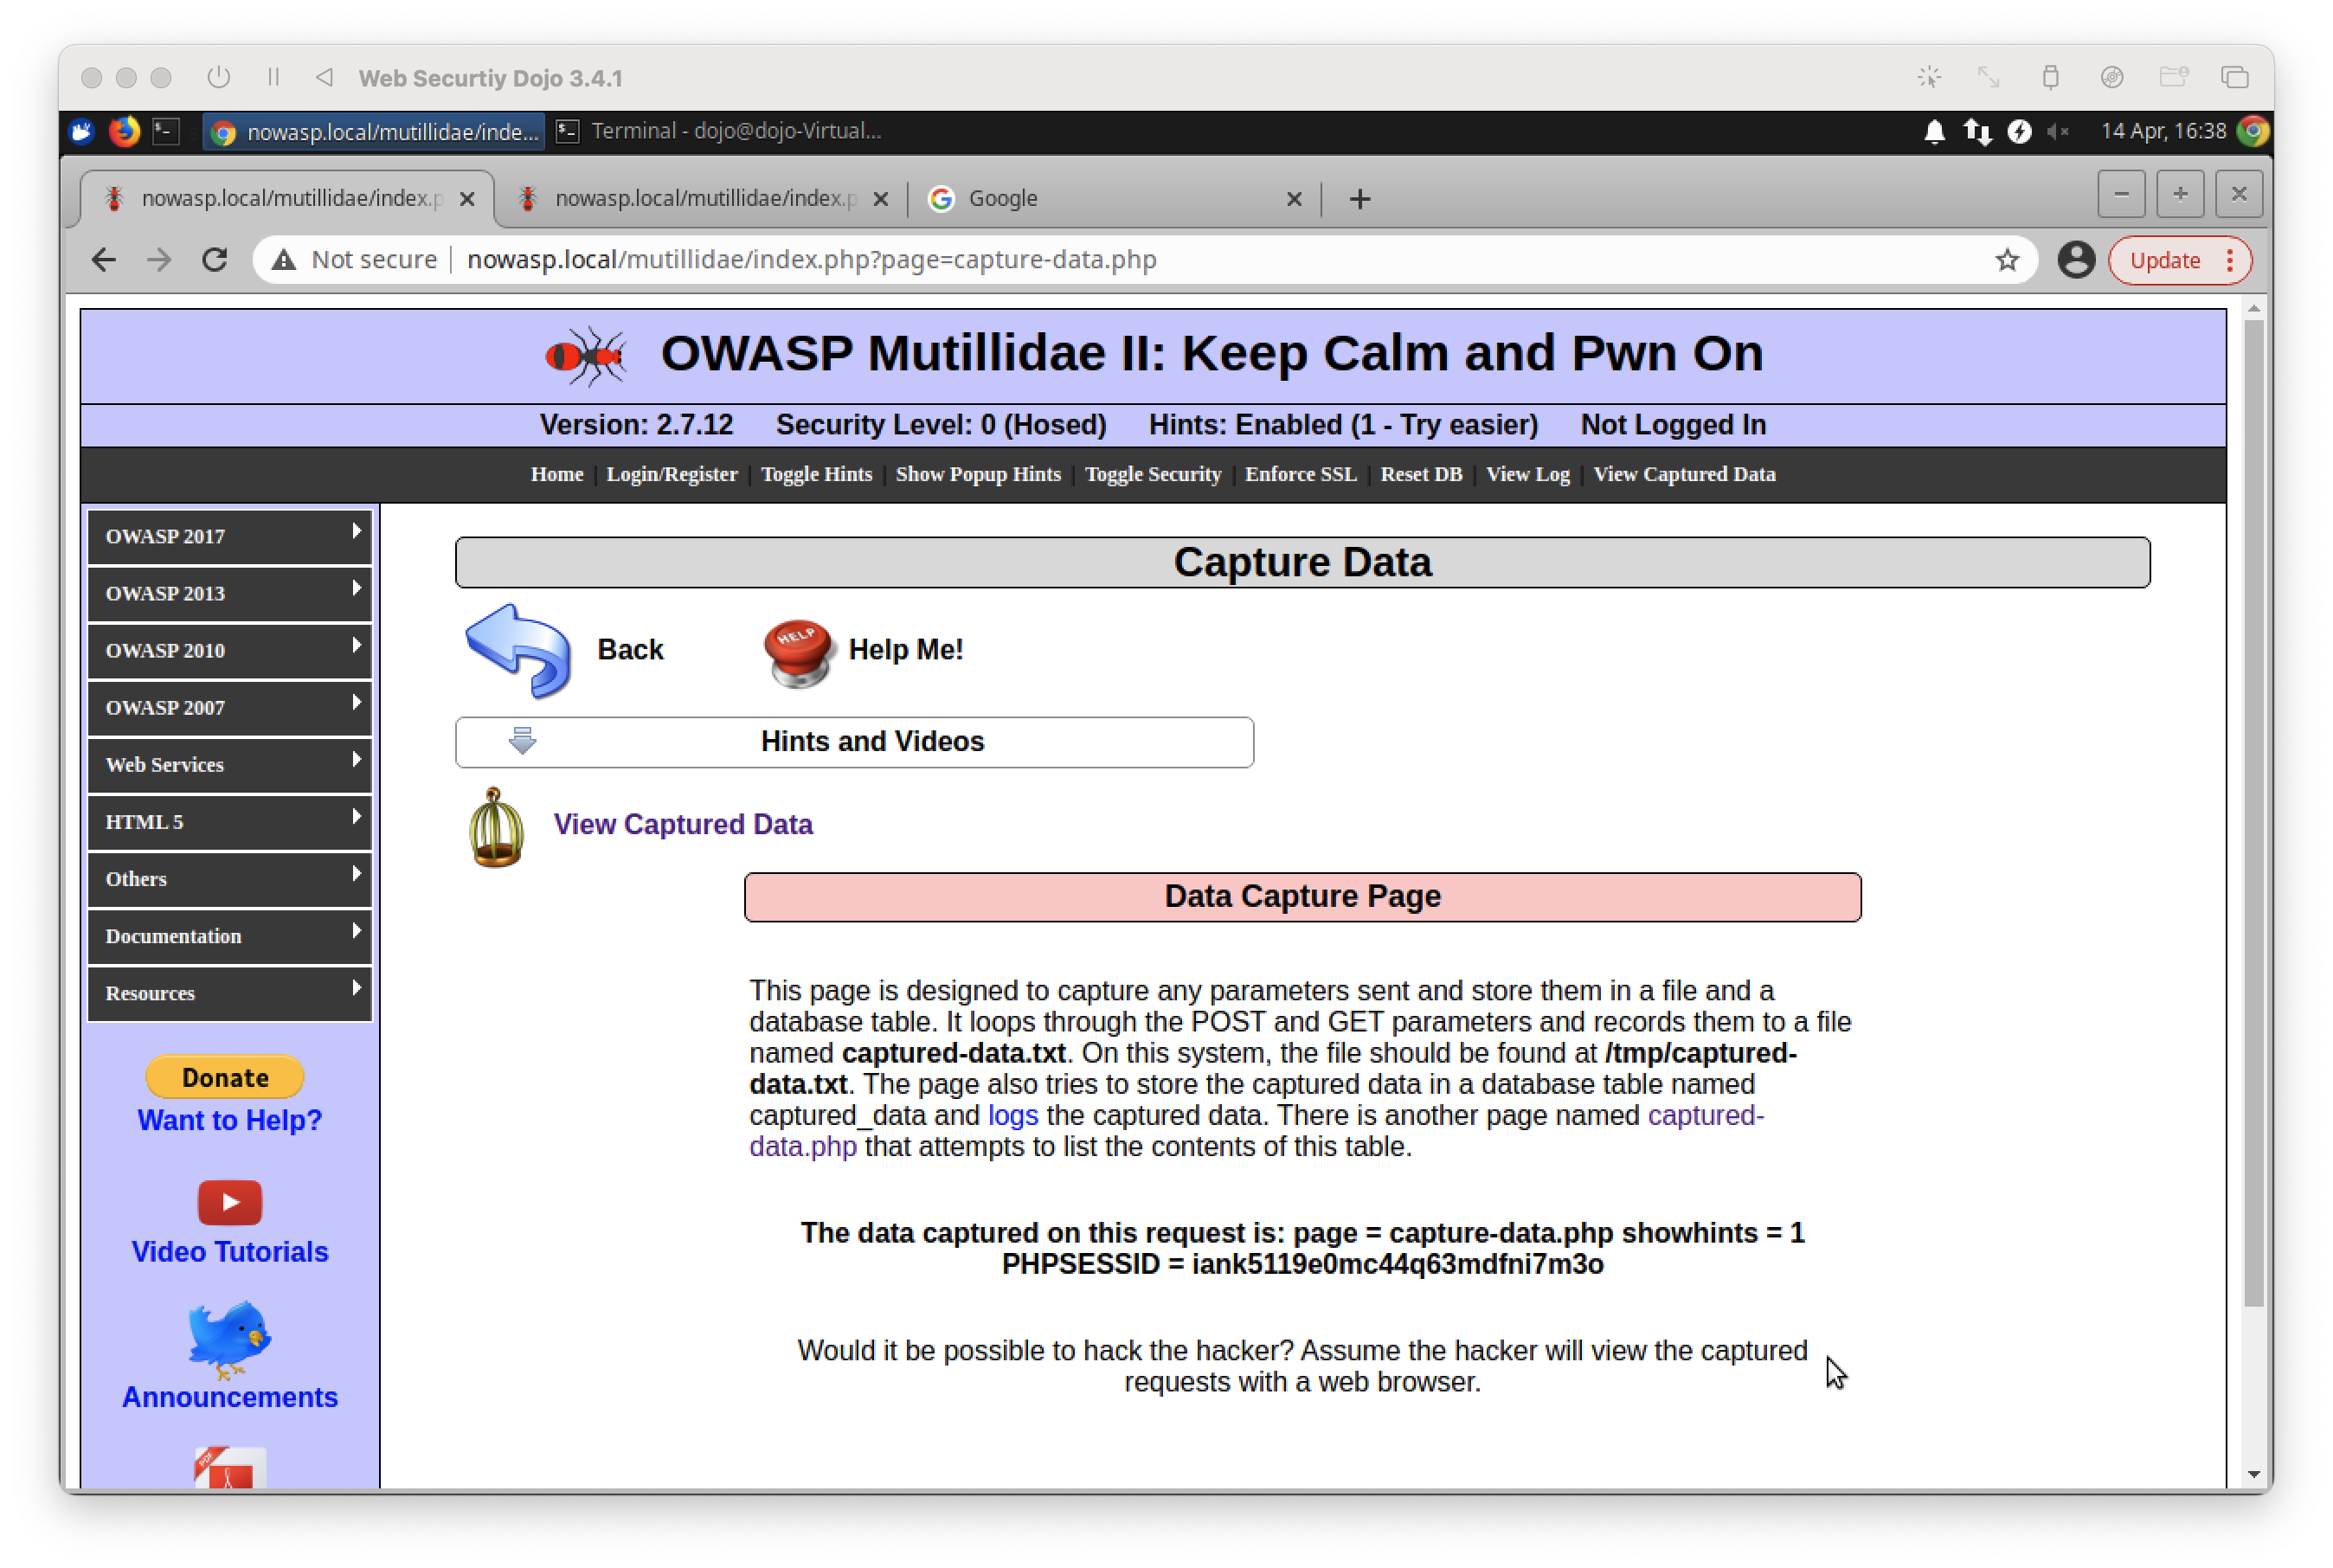
\includegraphics[width=0.8\textwidth]{step_00020}
    \caption{Видим страницу для атаки}
  \end{figure}

  Мы уже знаем, что она отобразит все переданные ей query-параметры, попробуем
  встроить код туда (в url):

  \begin{figure}[H]
    \centering
    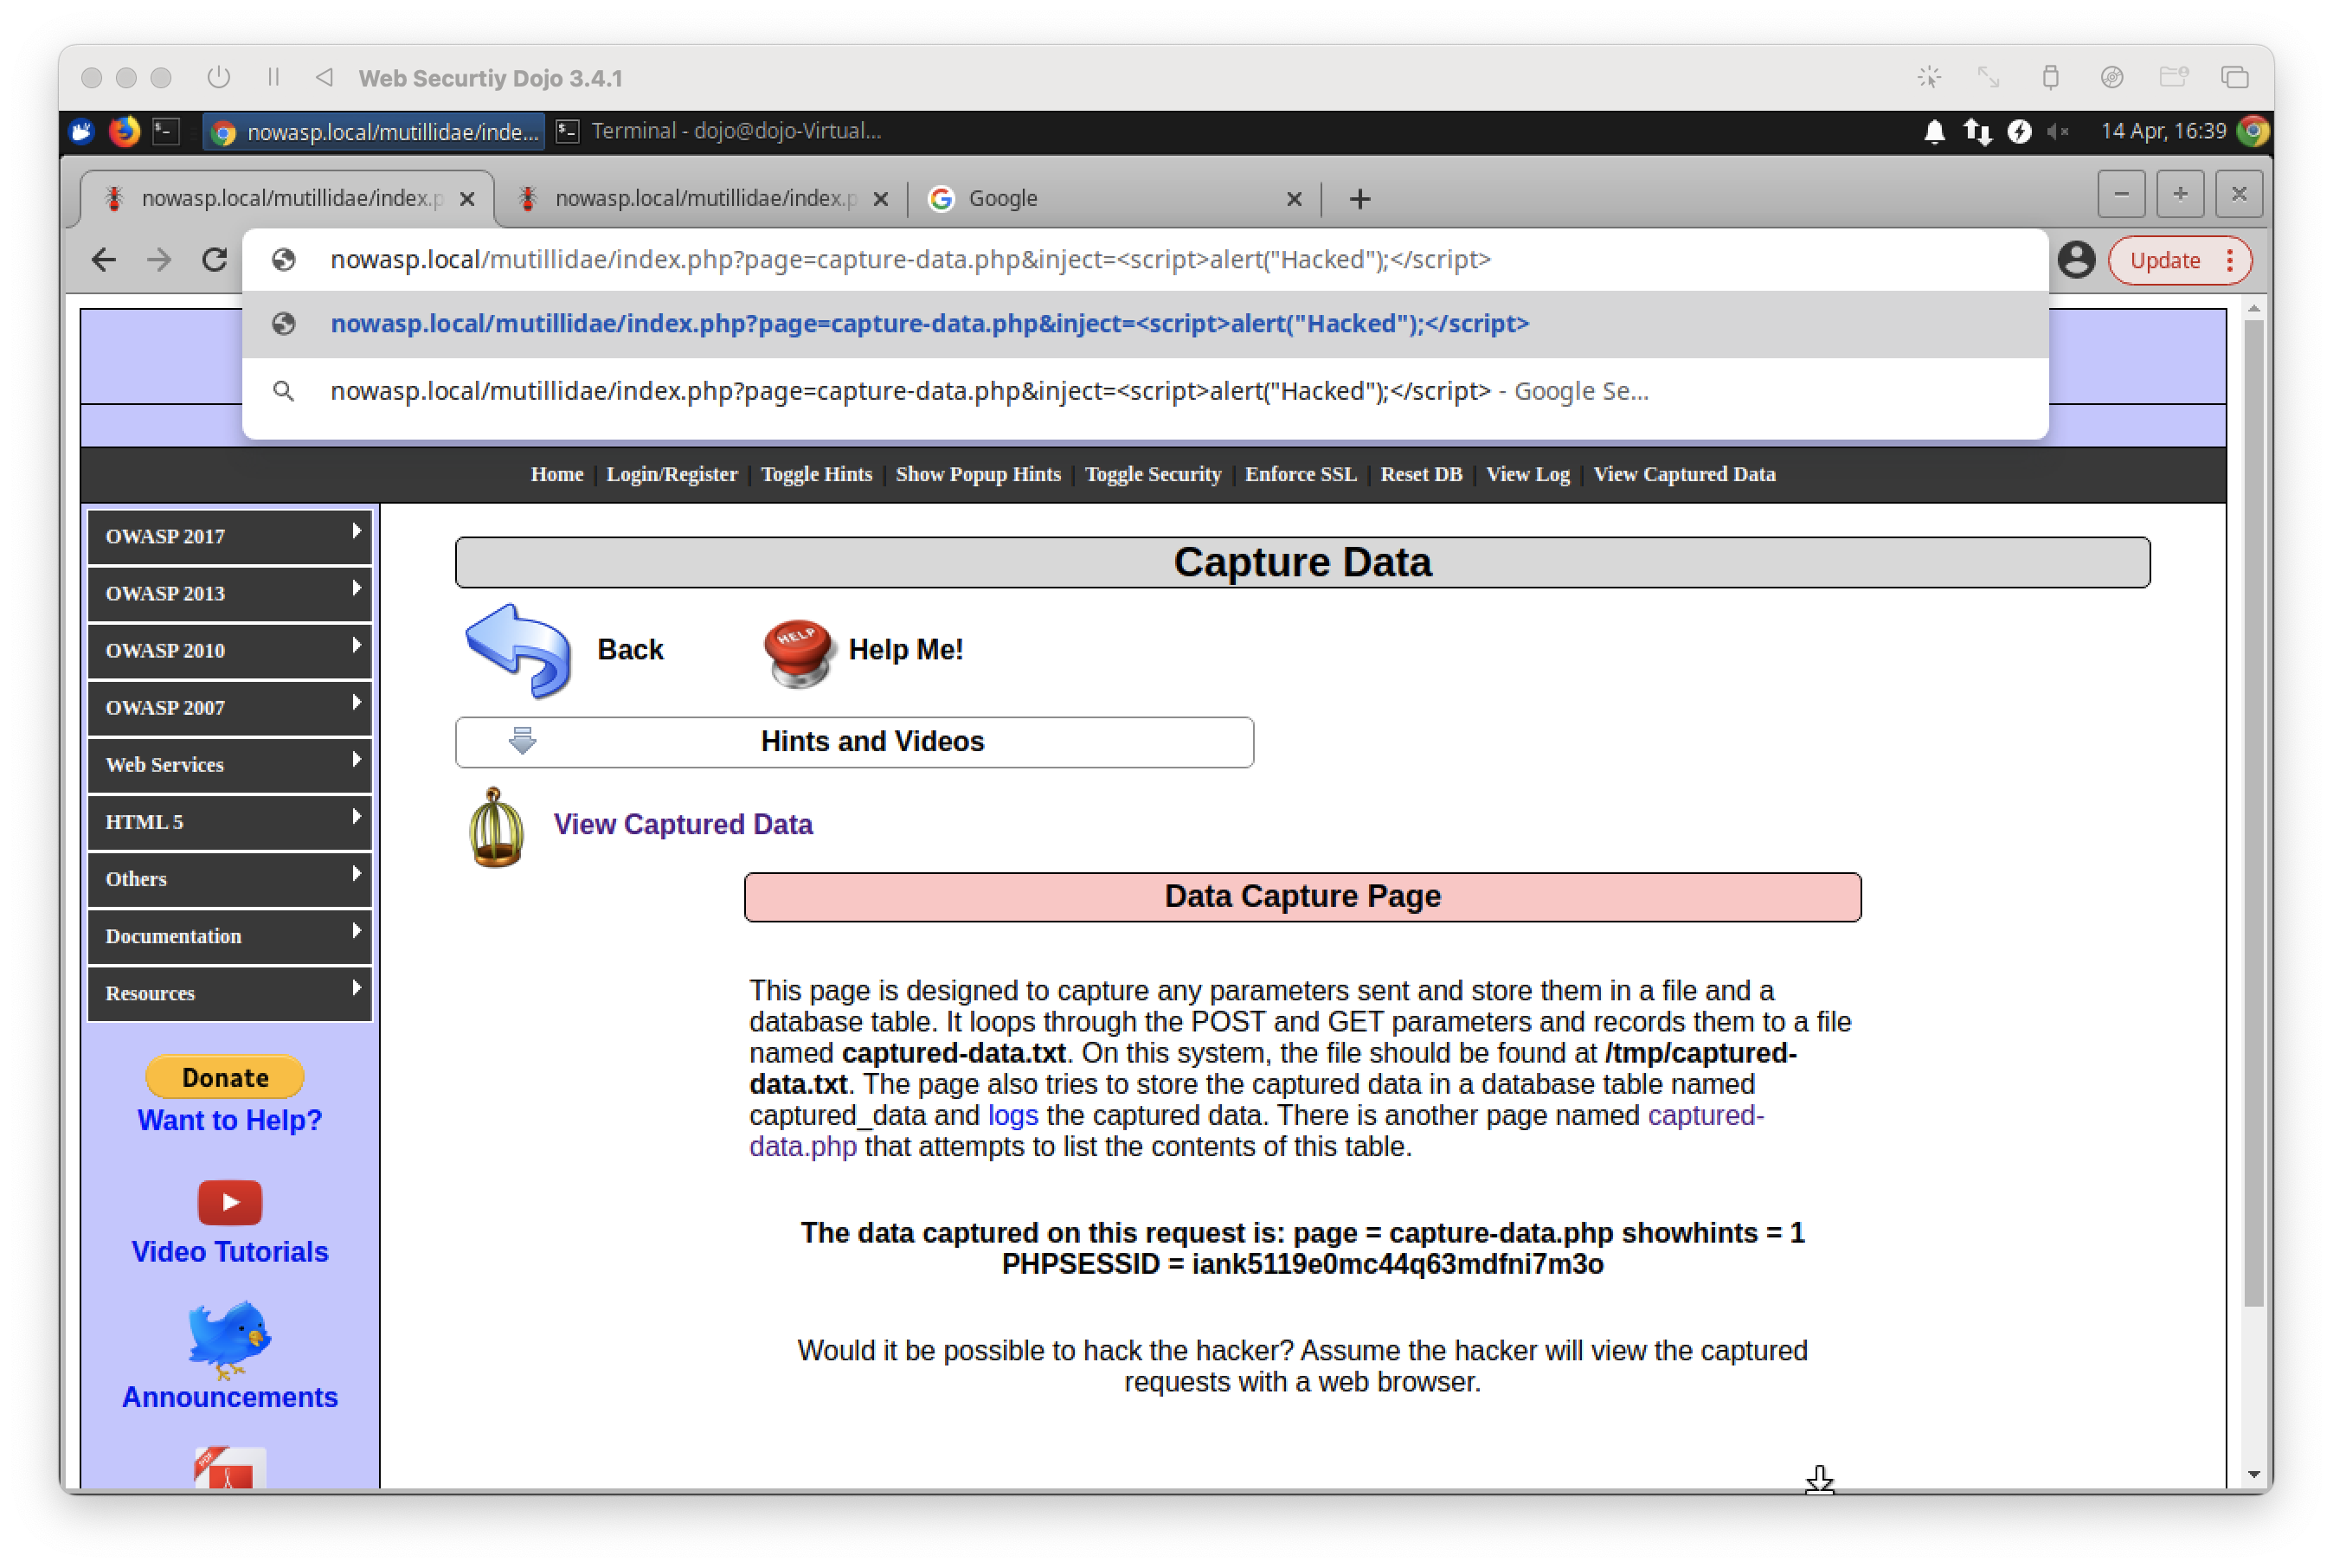
\includegraphics[width=0.8\textwidth]{step_00021}
    \caption{Добавляем новый query-параметр, значение которого - JS код внутри html тега script}
  \end{figure}

  \begin{figure}[H]
    \centering
    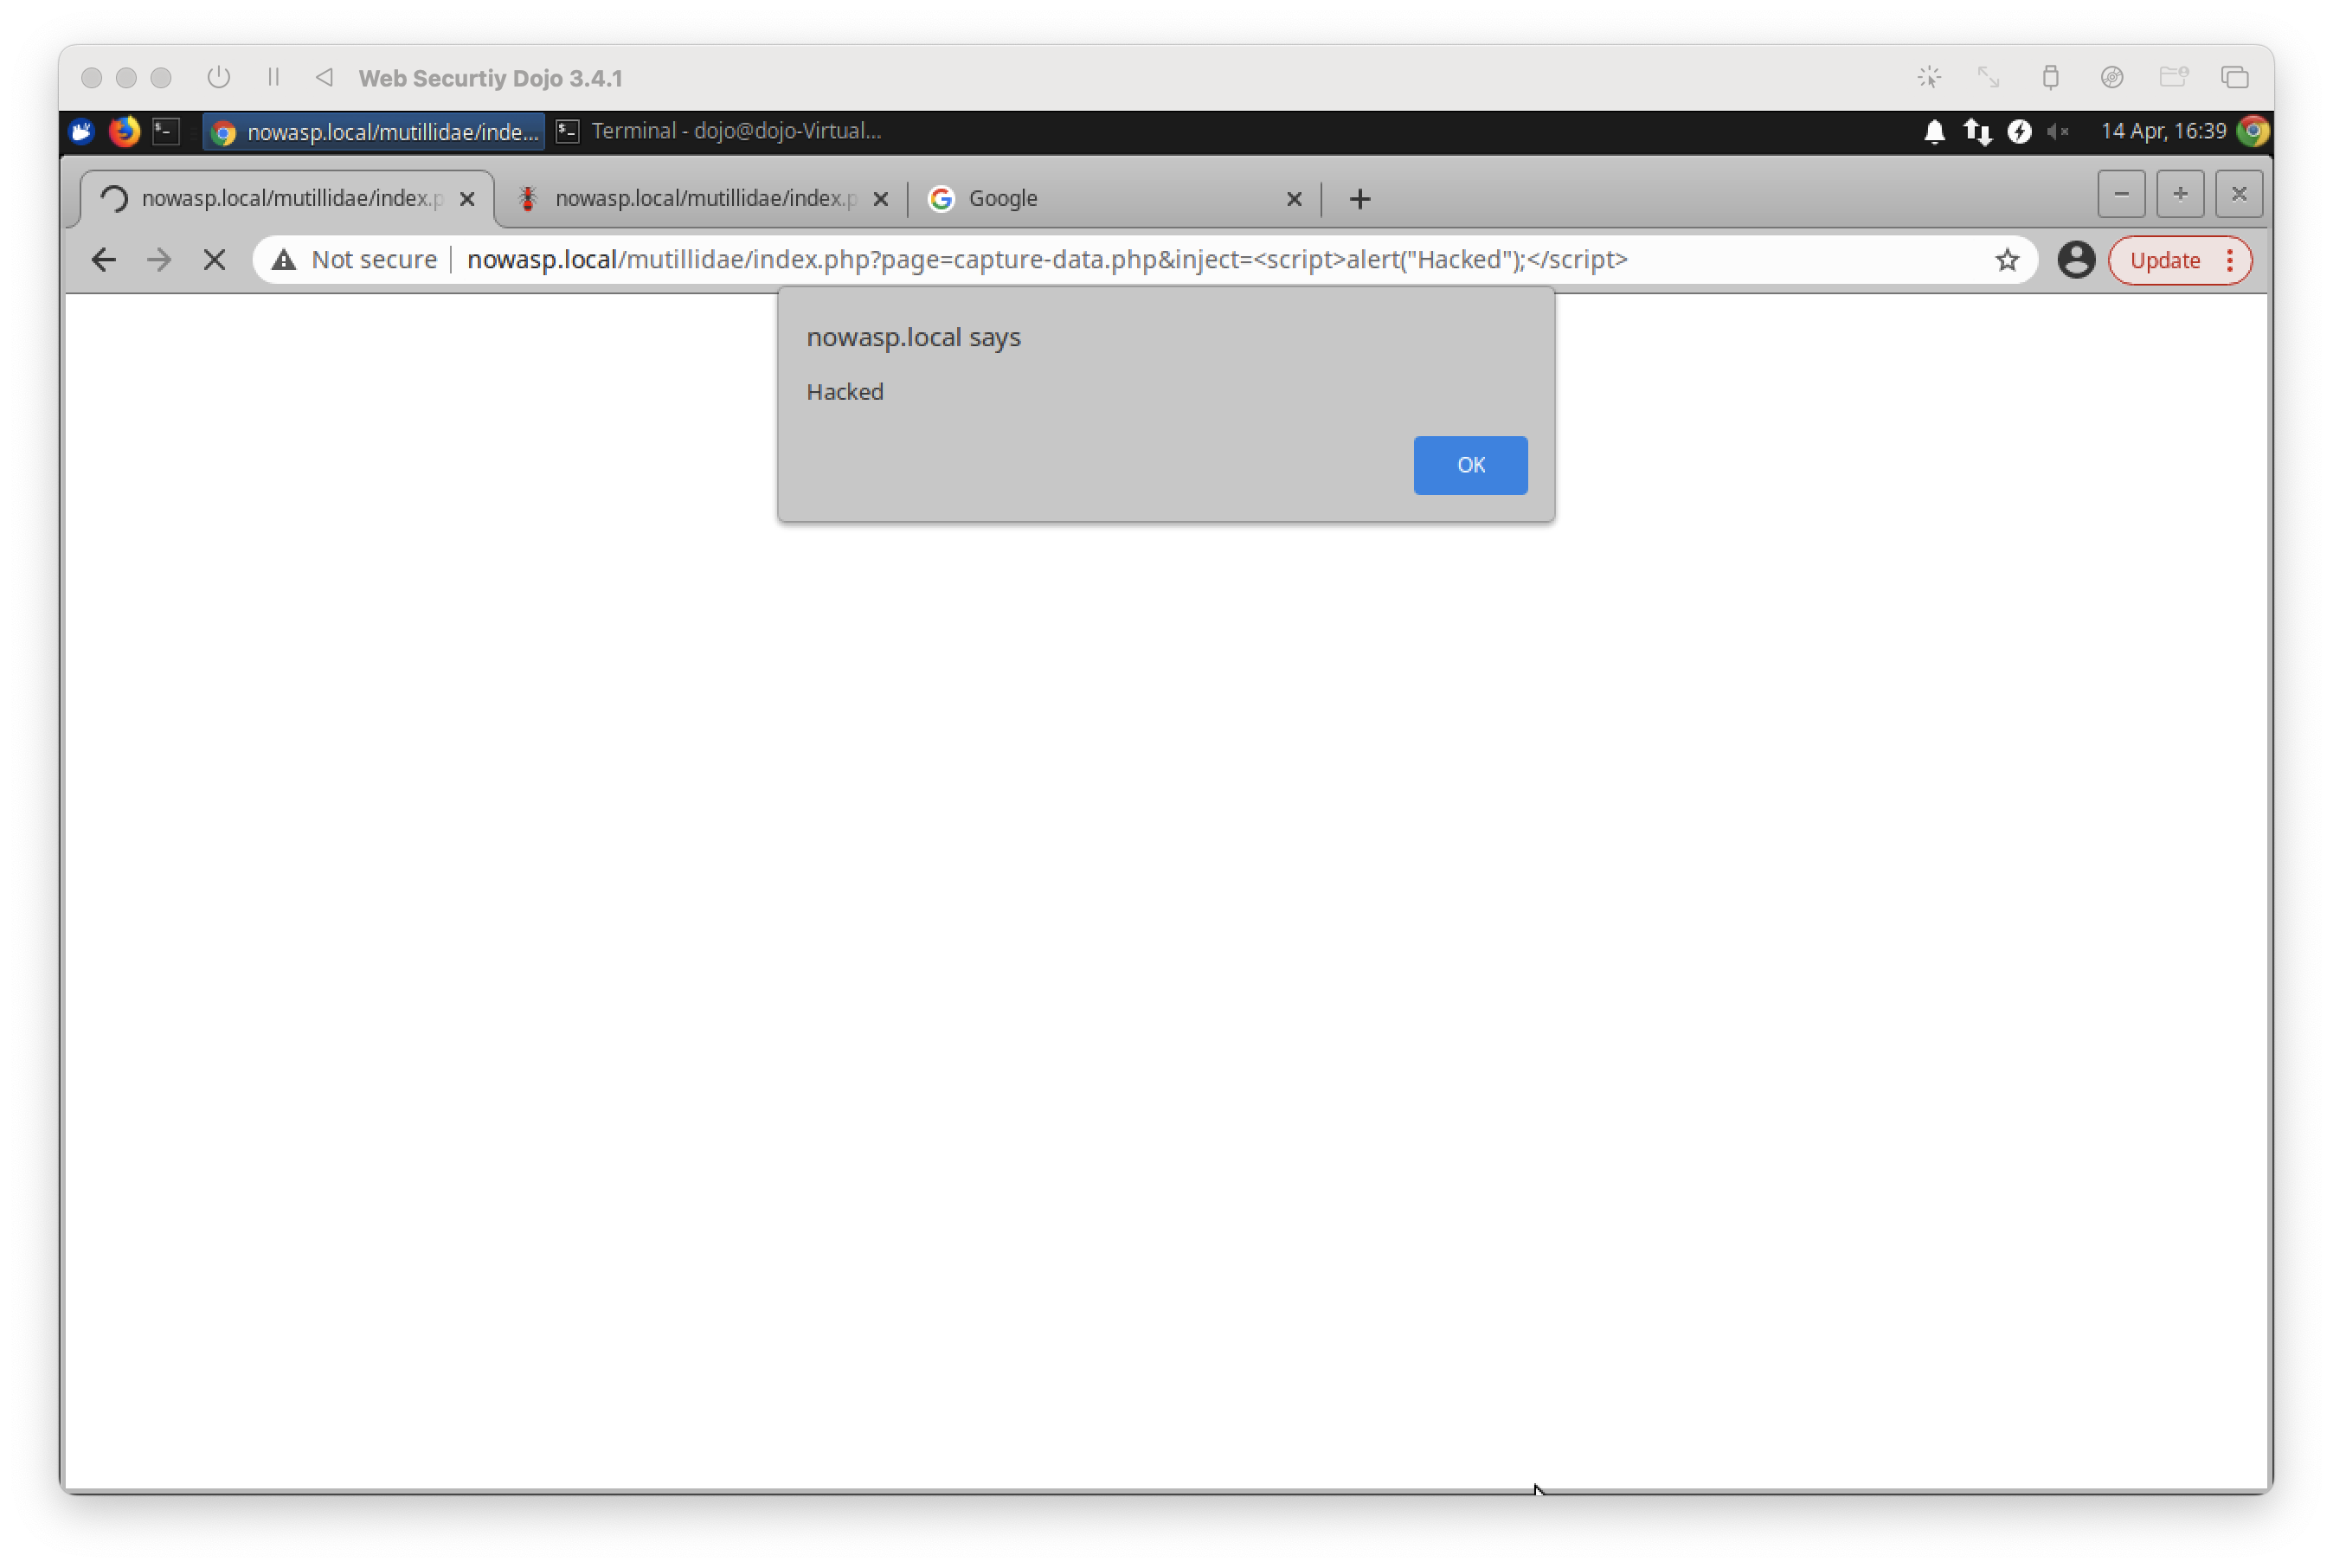
\includegraphics[width=0.8\textwidth]{step_00022}
    \caption{Сработало}
  \end{figure}

  \begin{figure}[H]
    \centering
    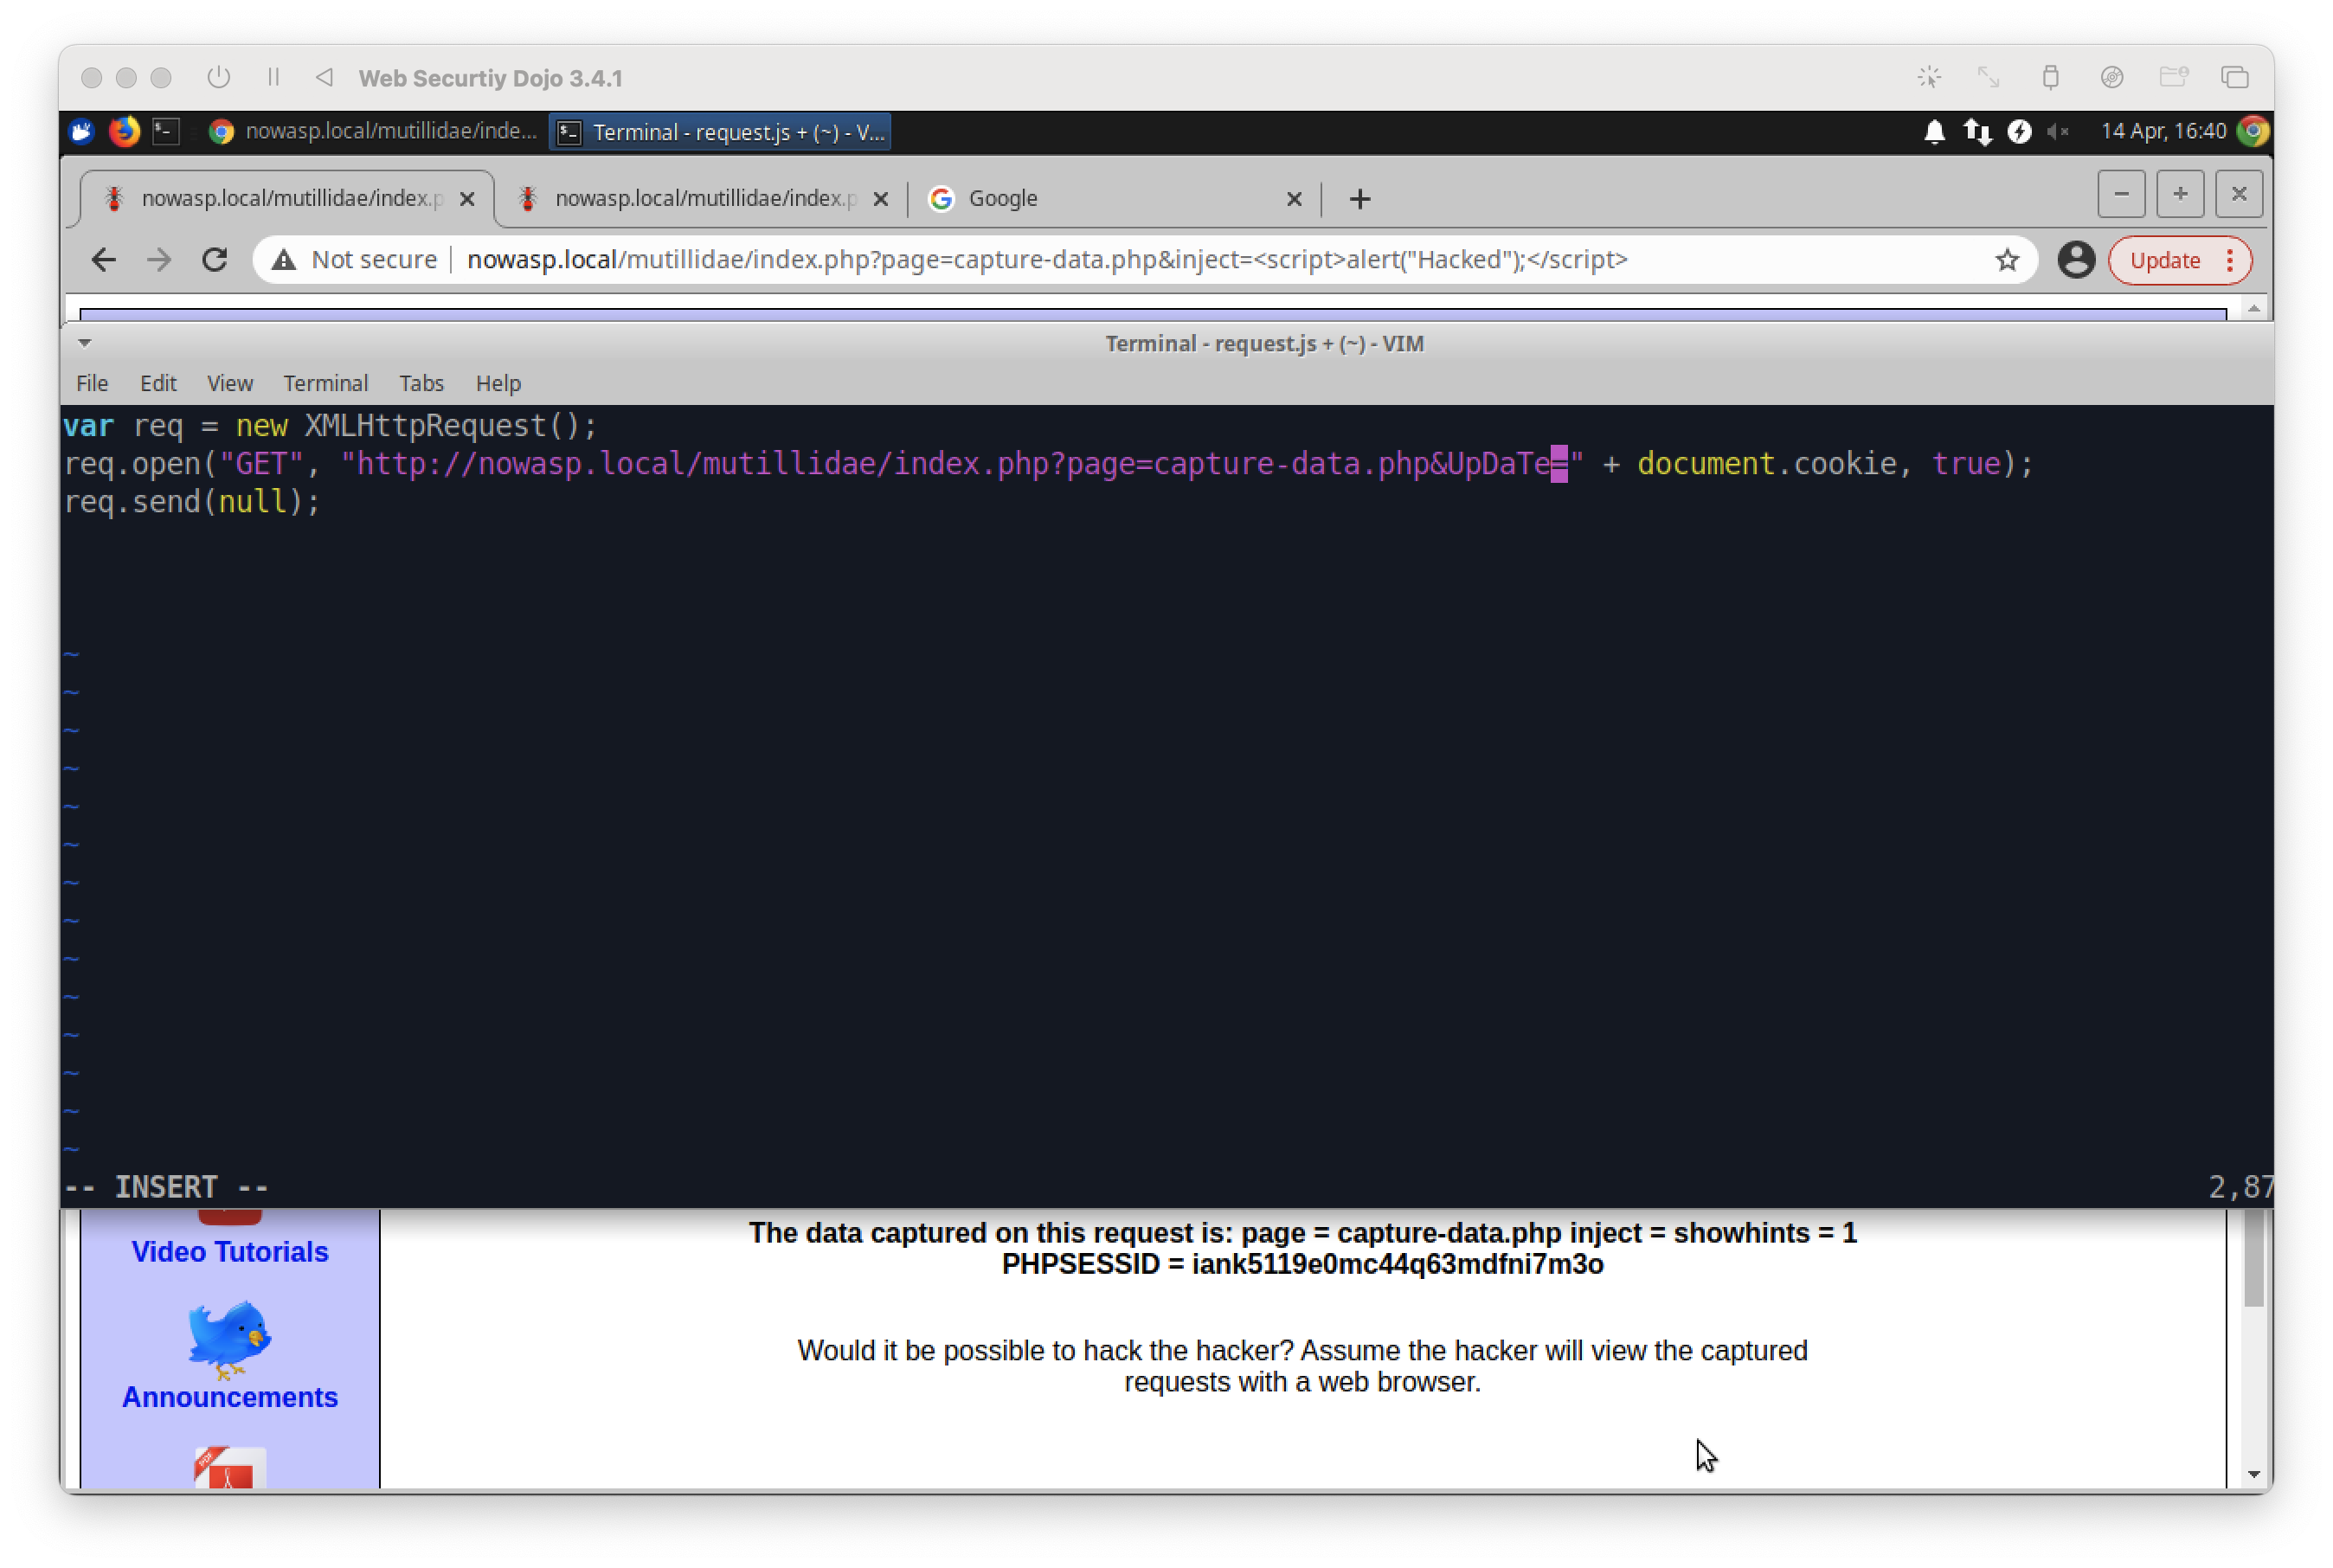
\includegraphics[width=0.8\textwidth]{step_00023}
    \caption{Попробуем встроить уже известный нам JS код для незаметной отправки (имя параметра изменилось, чтобы можно было отличить один запрос, от другого)}
  \end{figure}

  \begin{figure}[H]
    \centering
    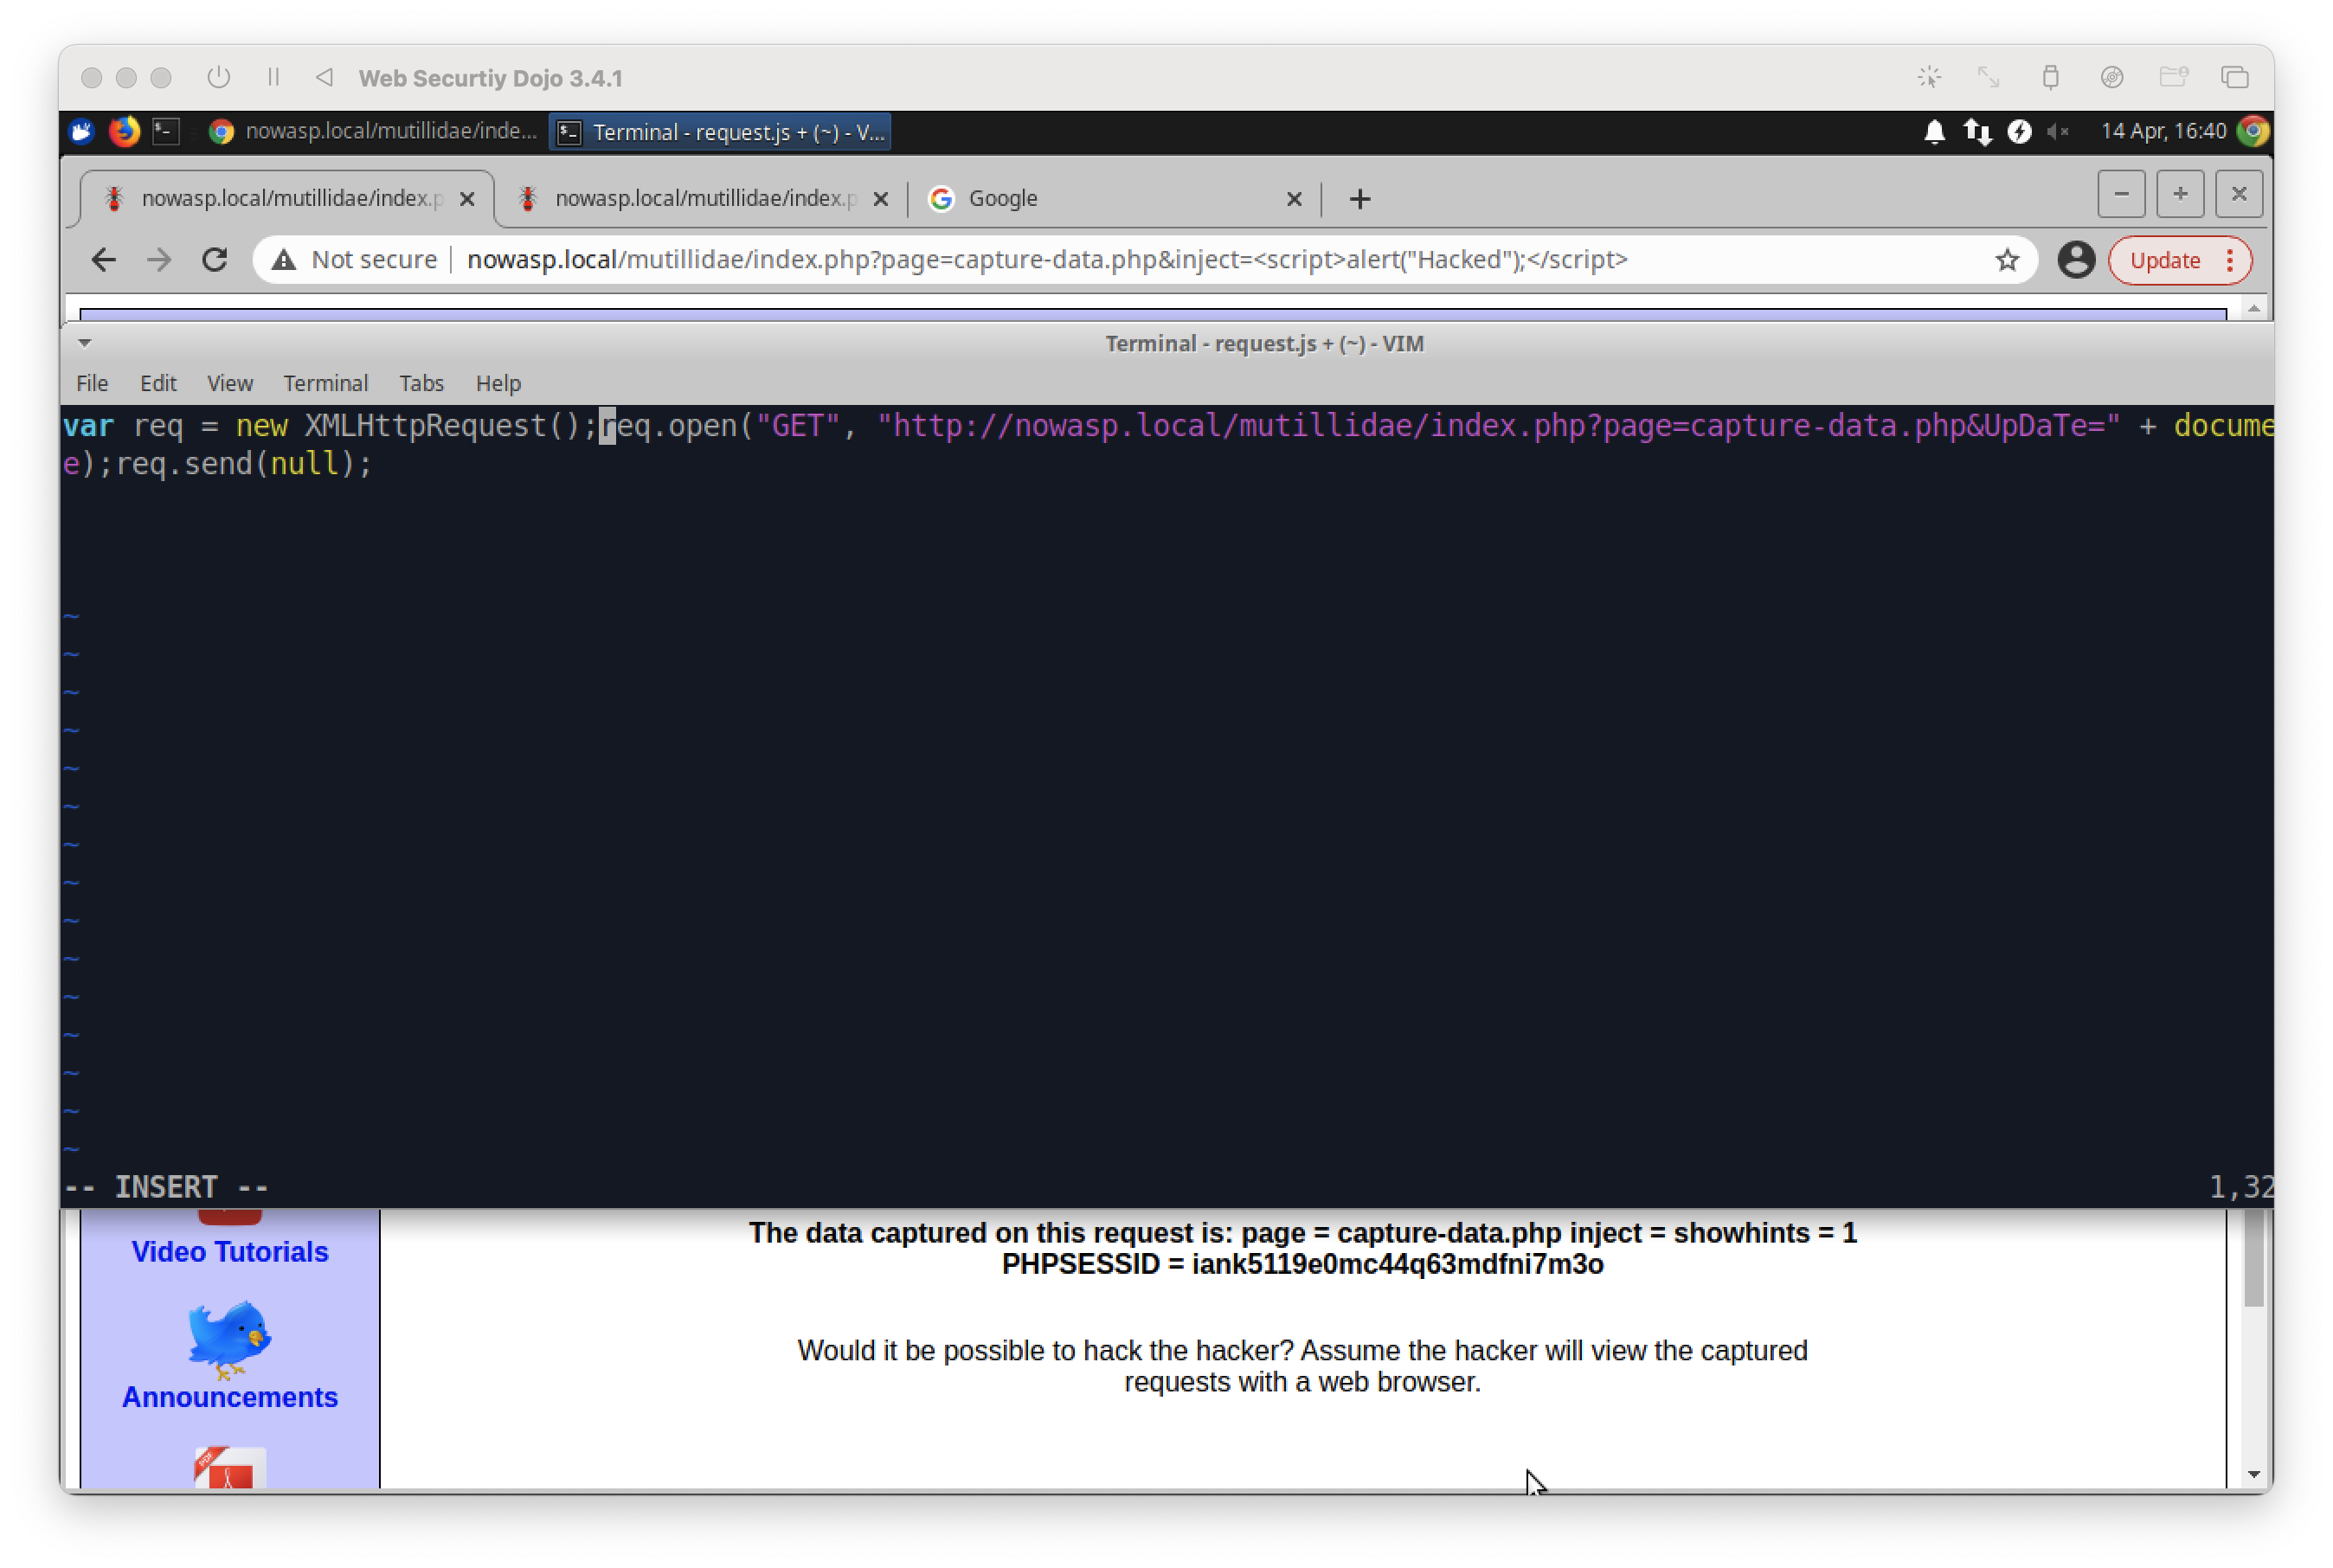
\includegraphics[width=0.8\textwidth]{step_00024}
    \caption{Понадобилось уместить всё в одну строку для удобства встраивания}
  \end{figure}

  \begin{figure}[H]
    \centering
    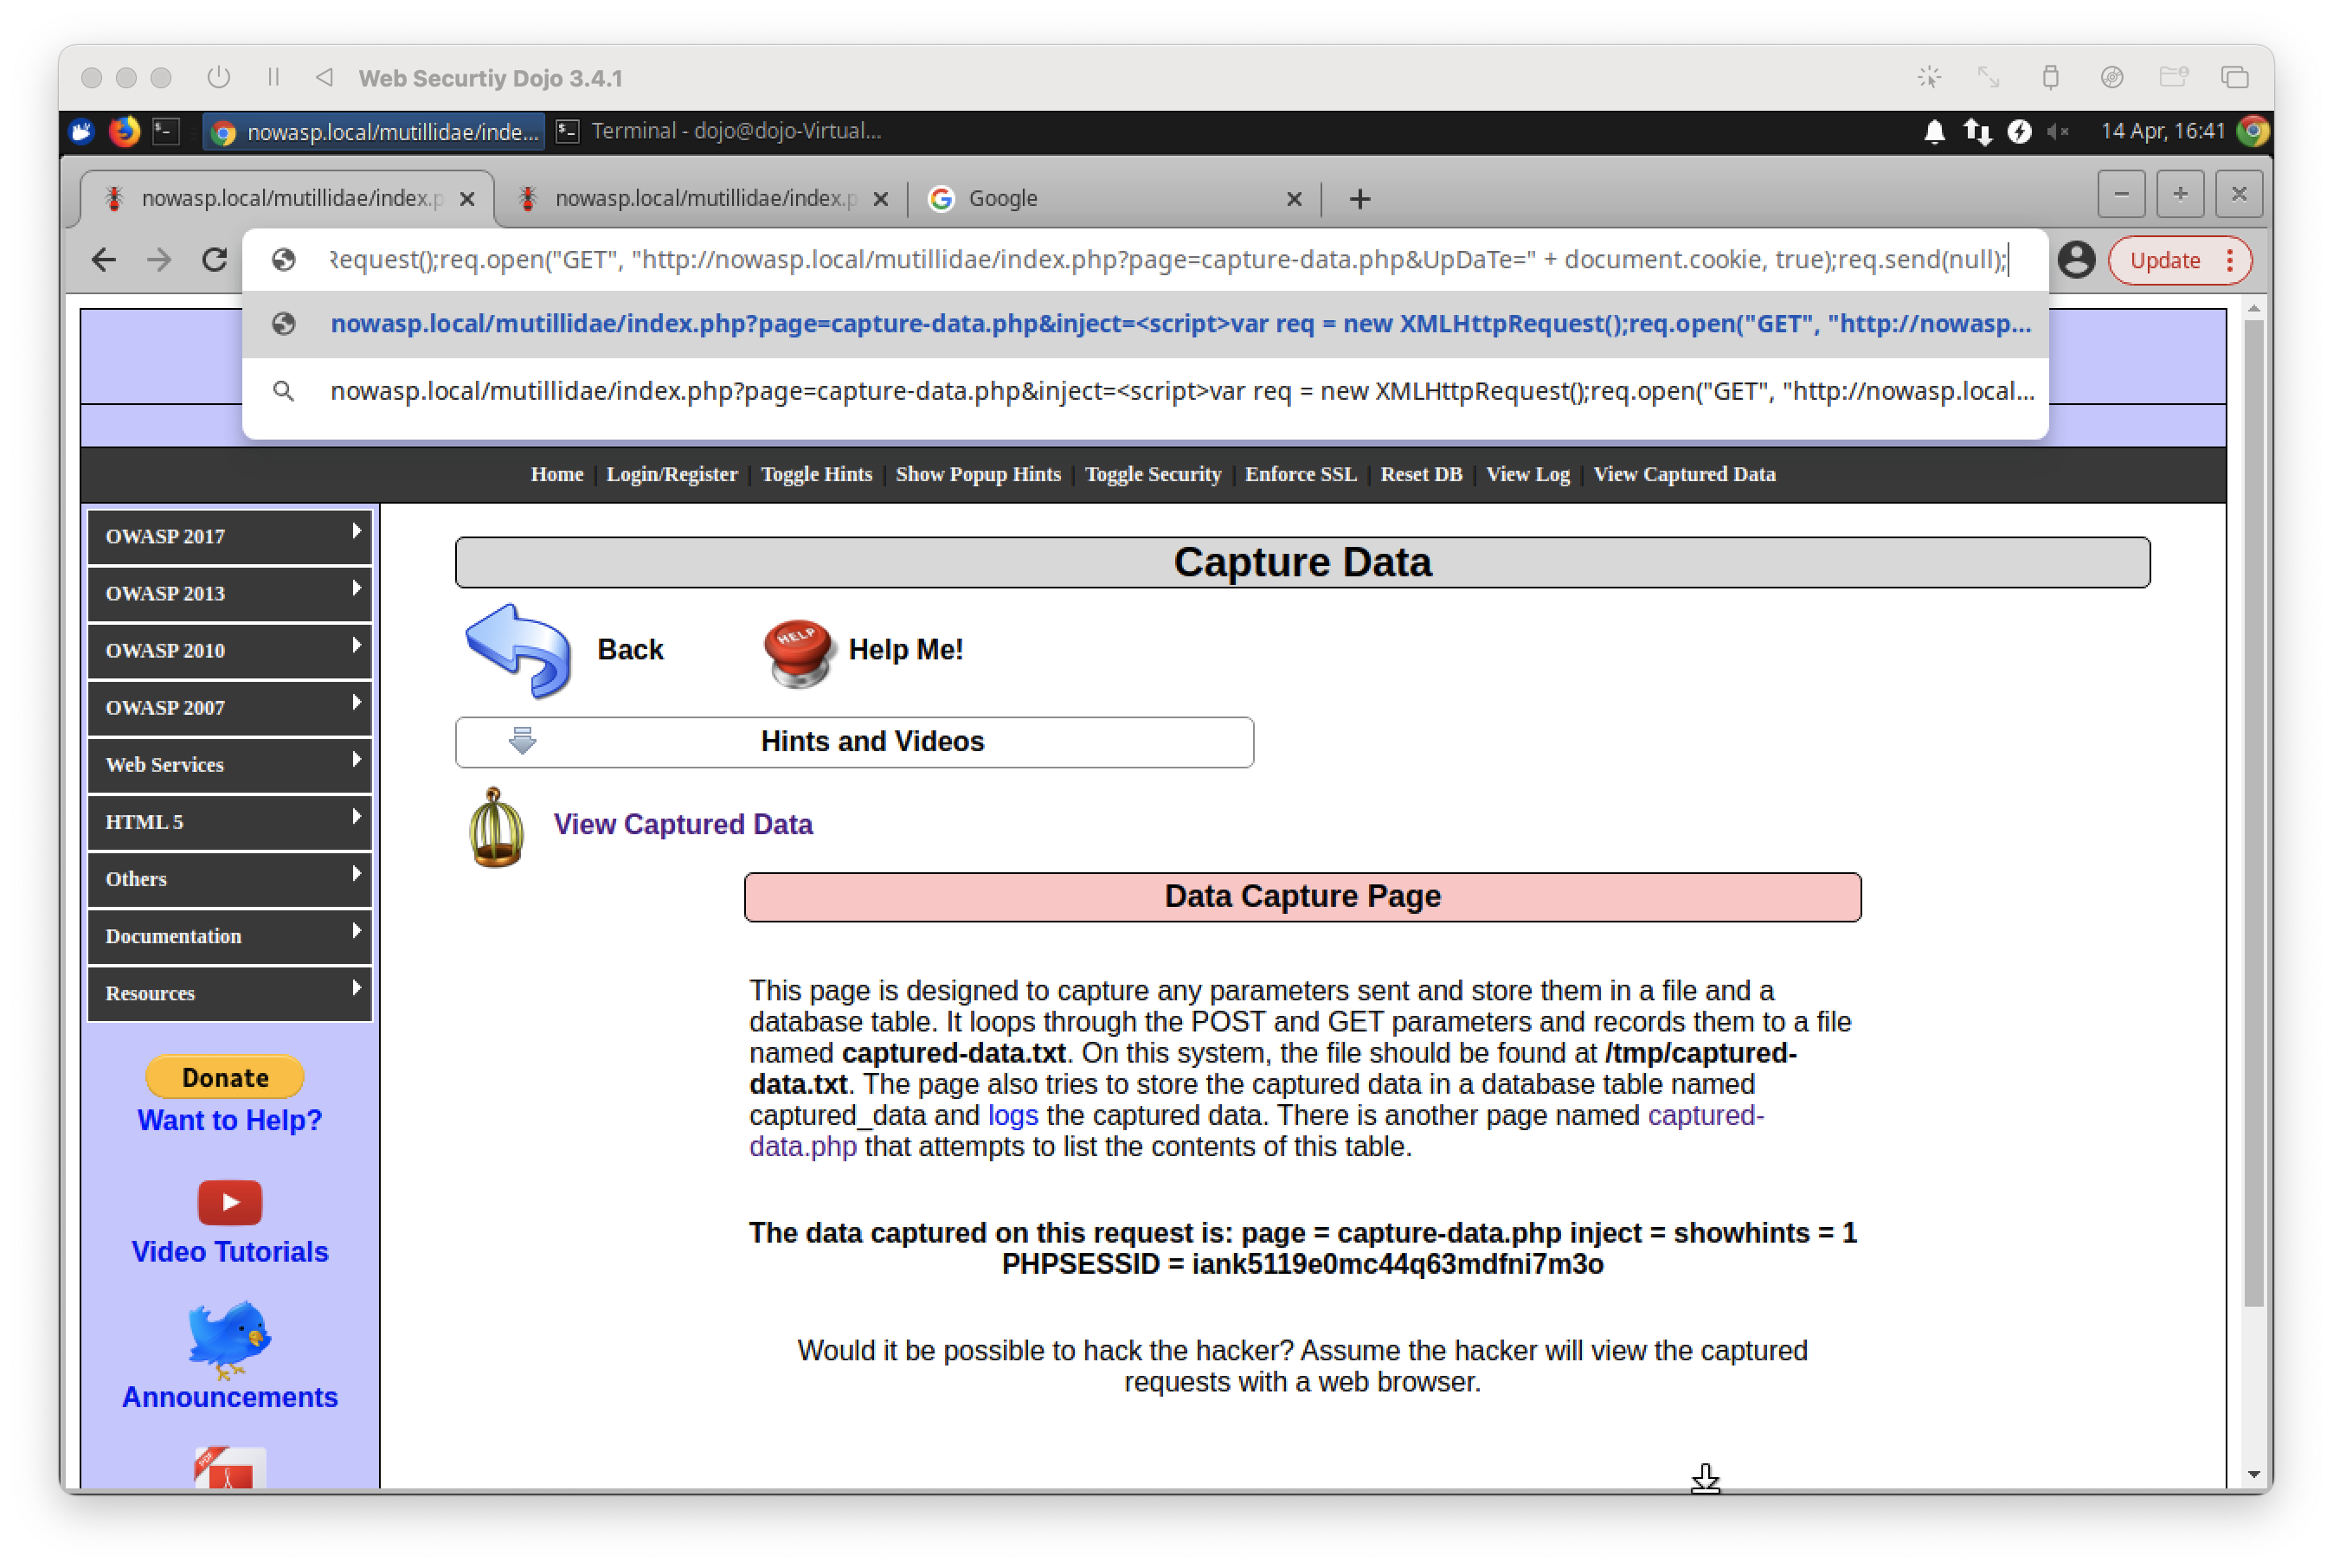
\includegraphics[width=0.8\textwidth]{step_00025}
    \caption{Пробуем встроить полноценный JS внутрь url}
  \end{figure}

  \begin{figure}[H]
    \centering
    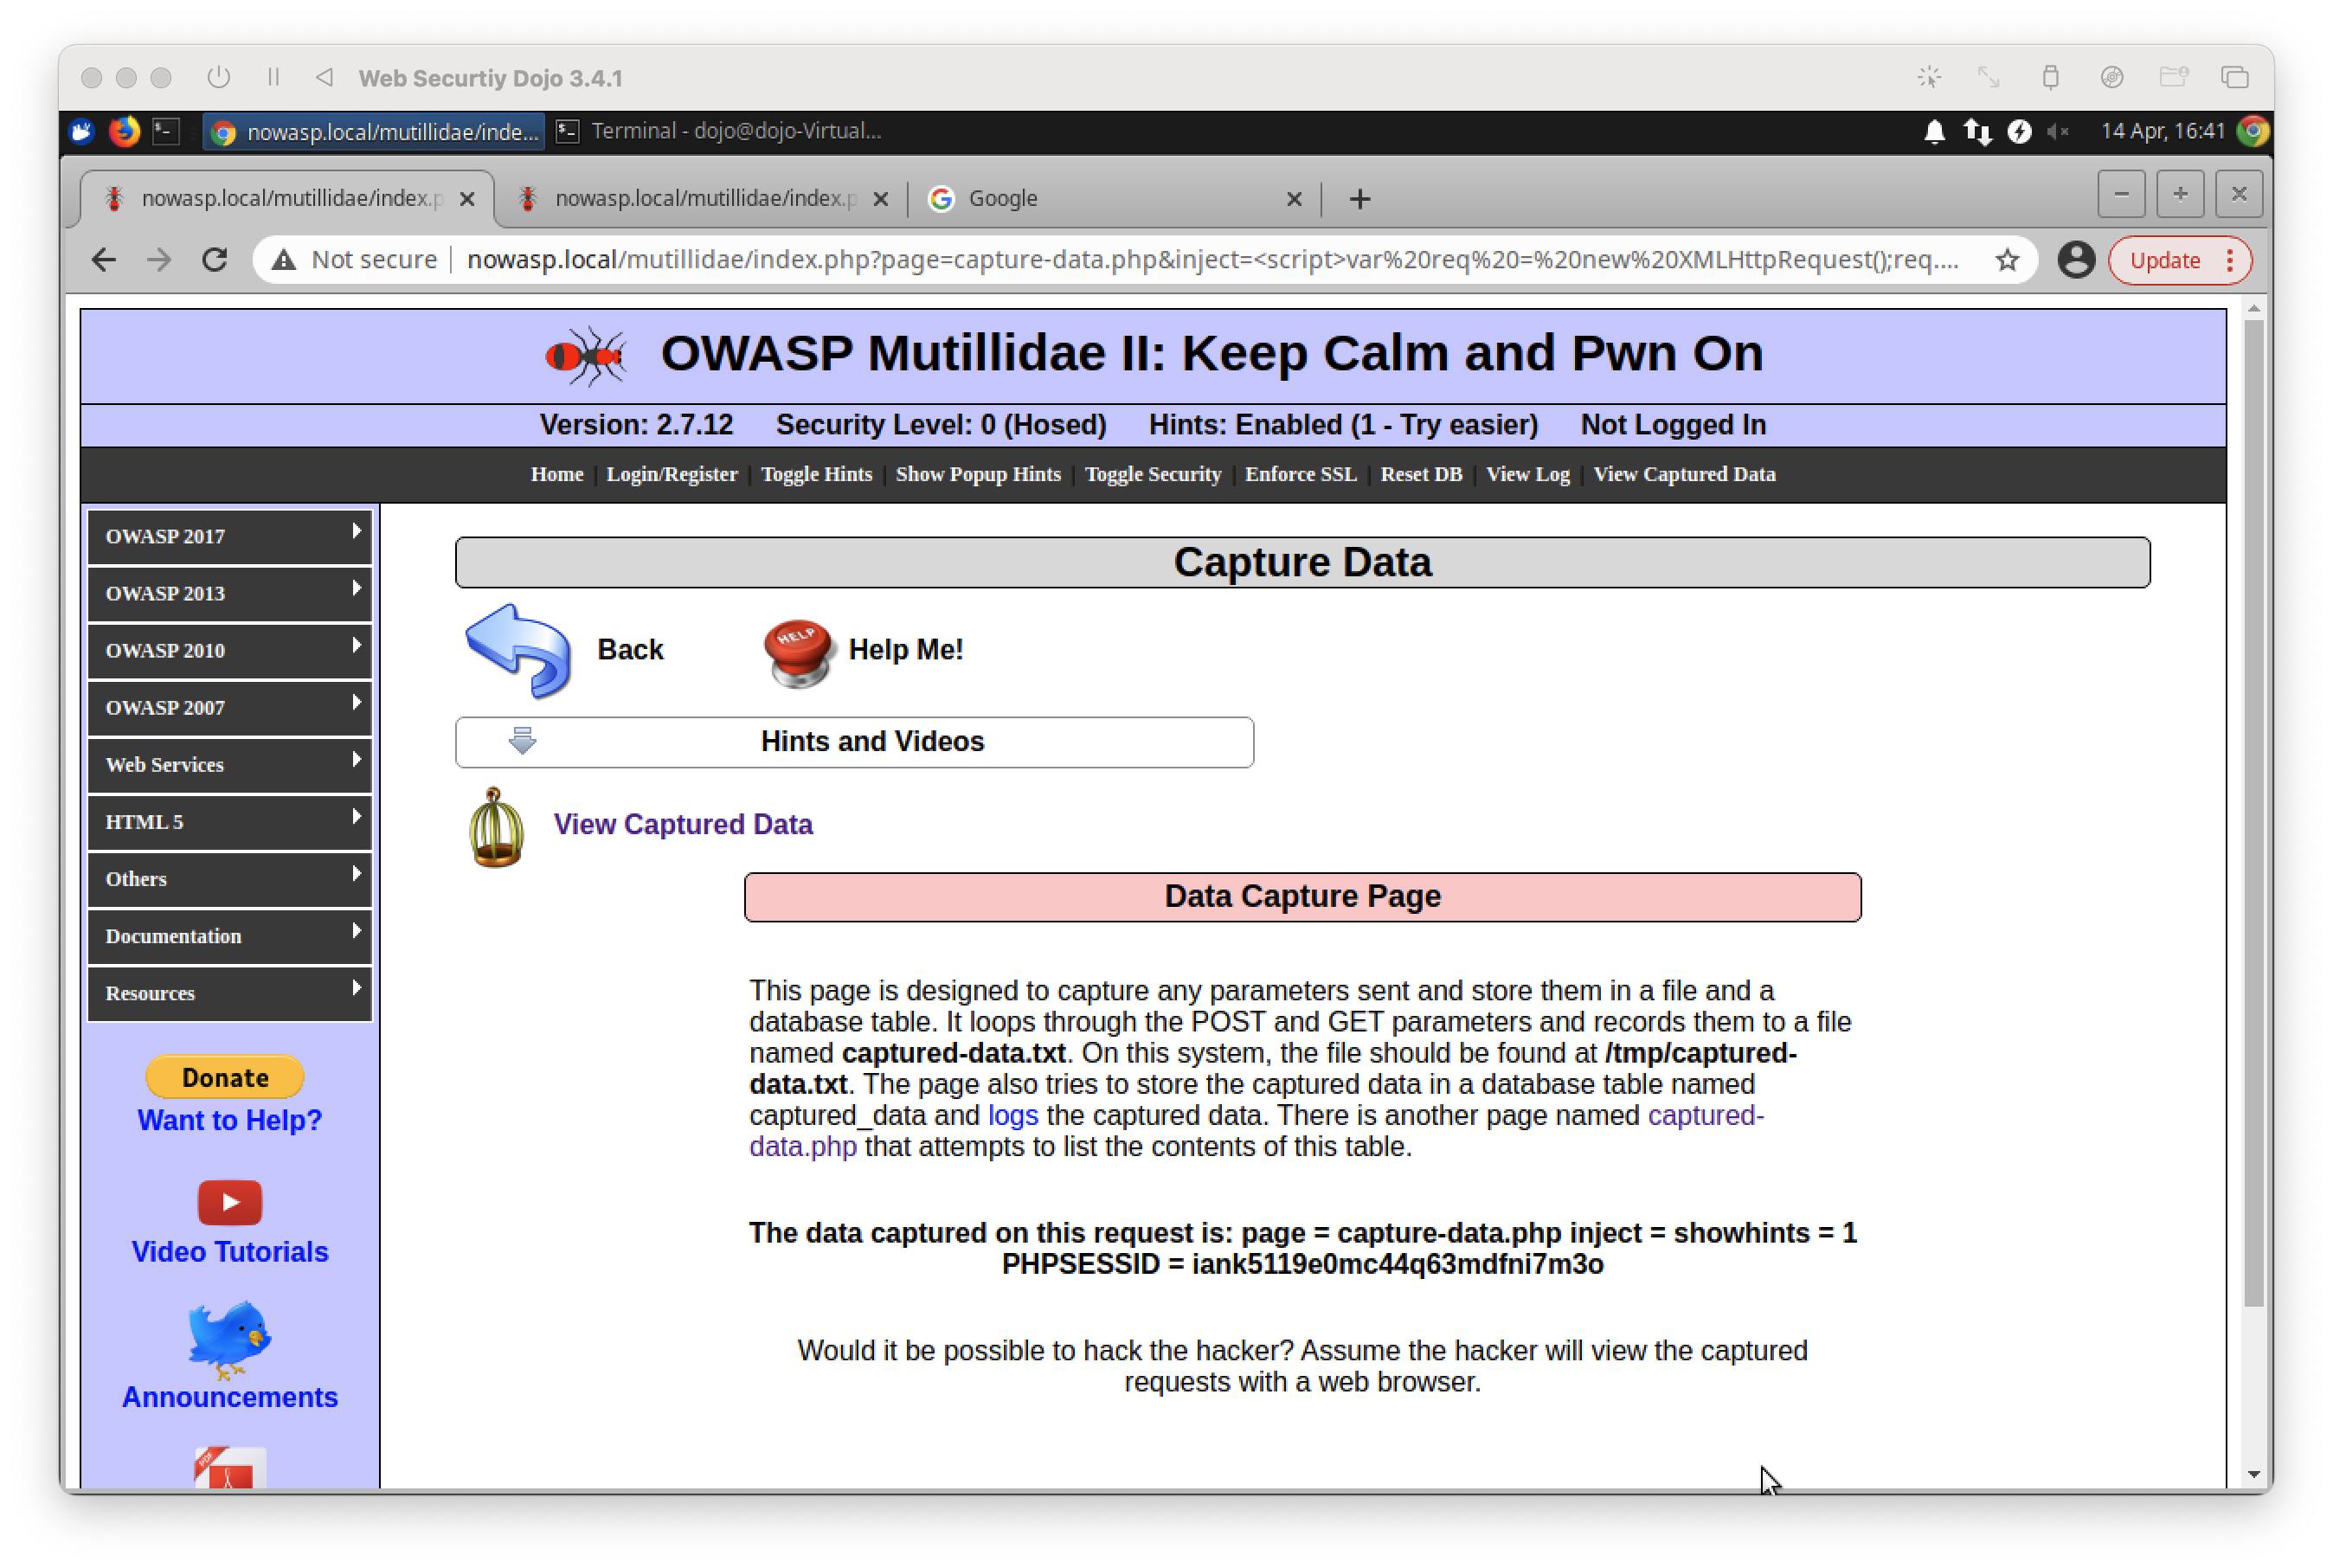
\includegraphics[width=0.8\textwidth]{step_00026}
    \caption{Страница загрузилась, но случилось ли что-то?}
  \end{figure}

  Как оказалось - код для атаки был встроен неправильно, потому что в 
  нём содержались символы, которые нельзя передавть внутри url в явном виде:

  \begin{figure}[H]
    \centering
    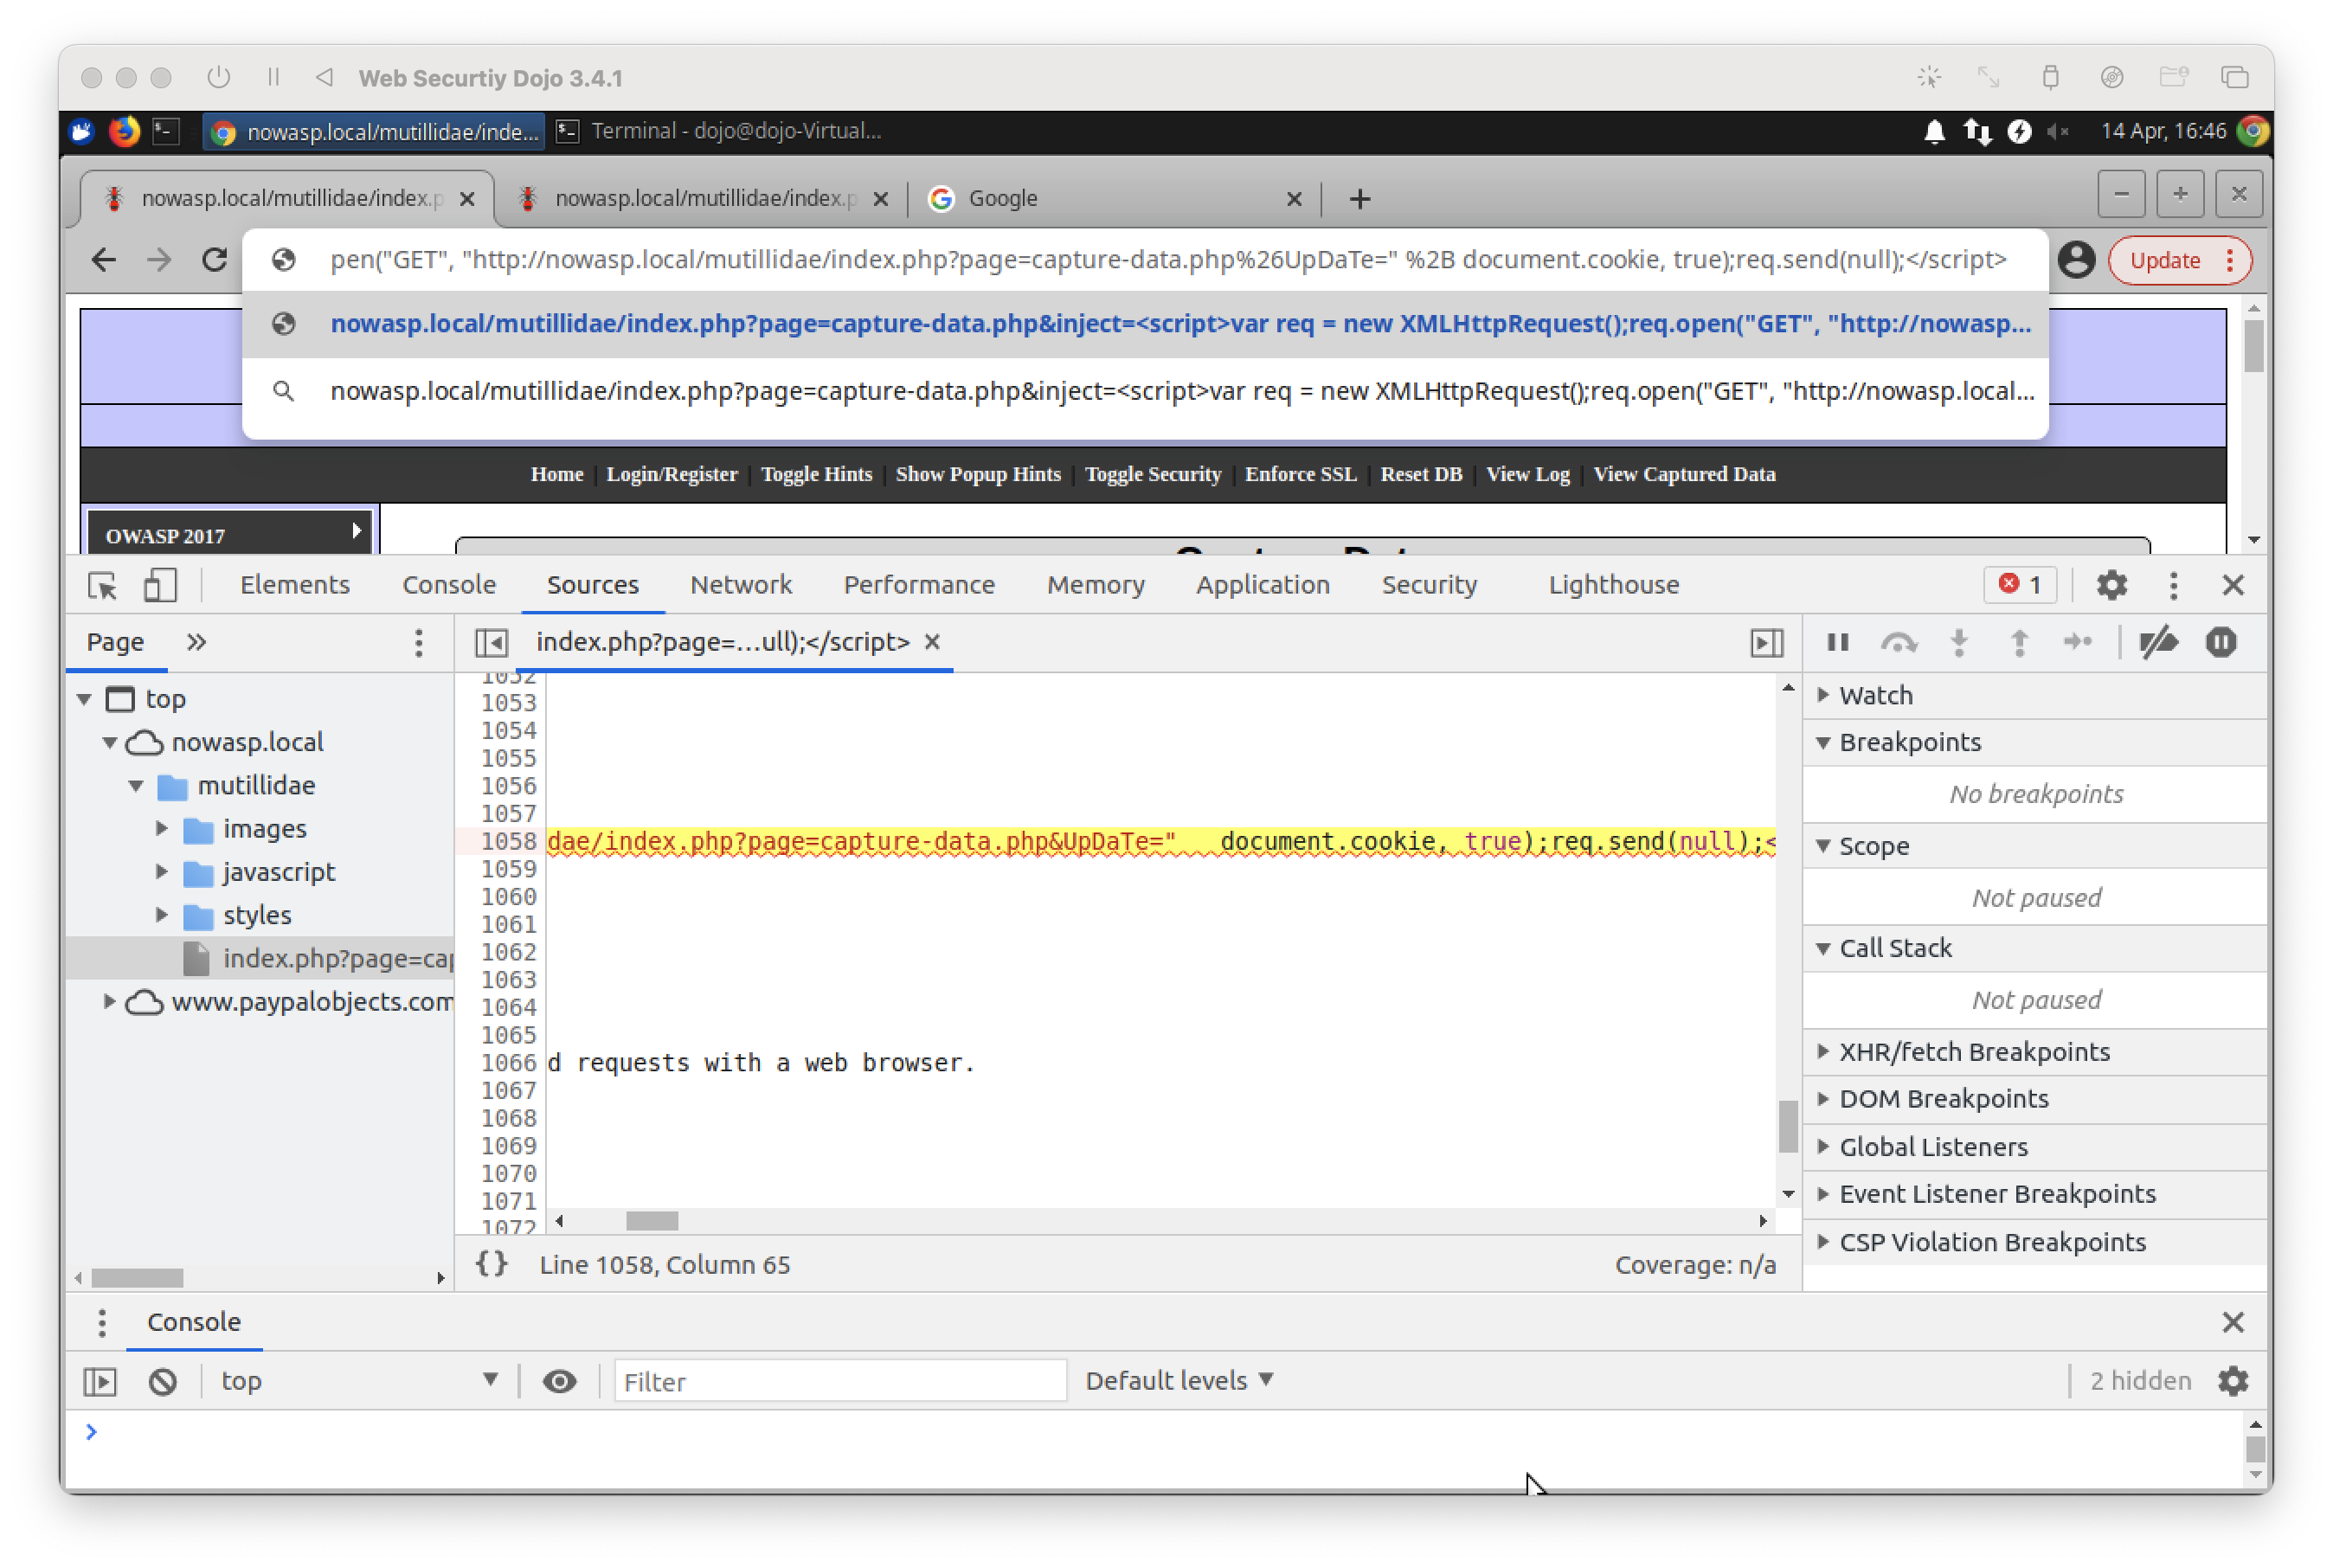
\includegraphics[width=0.8\textwidth]{step_00029}
    \caption{Поломанный код без плюса}
  \end{figure}

  Заменяем внутри url знак $+$ на эквивалентный ему код $\%26$

  \begin{figure}[H]
    \centering
    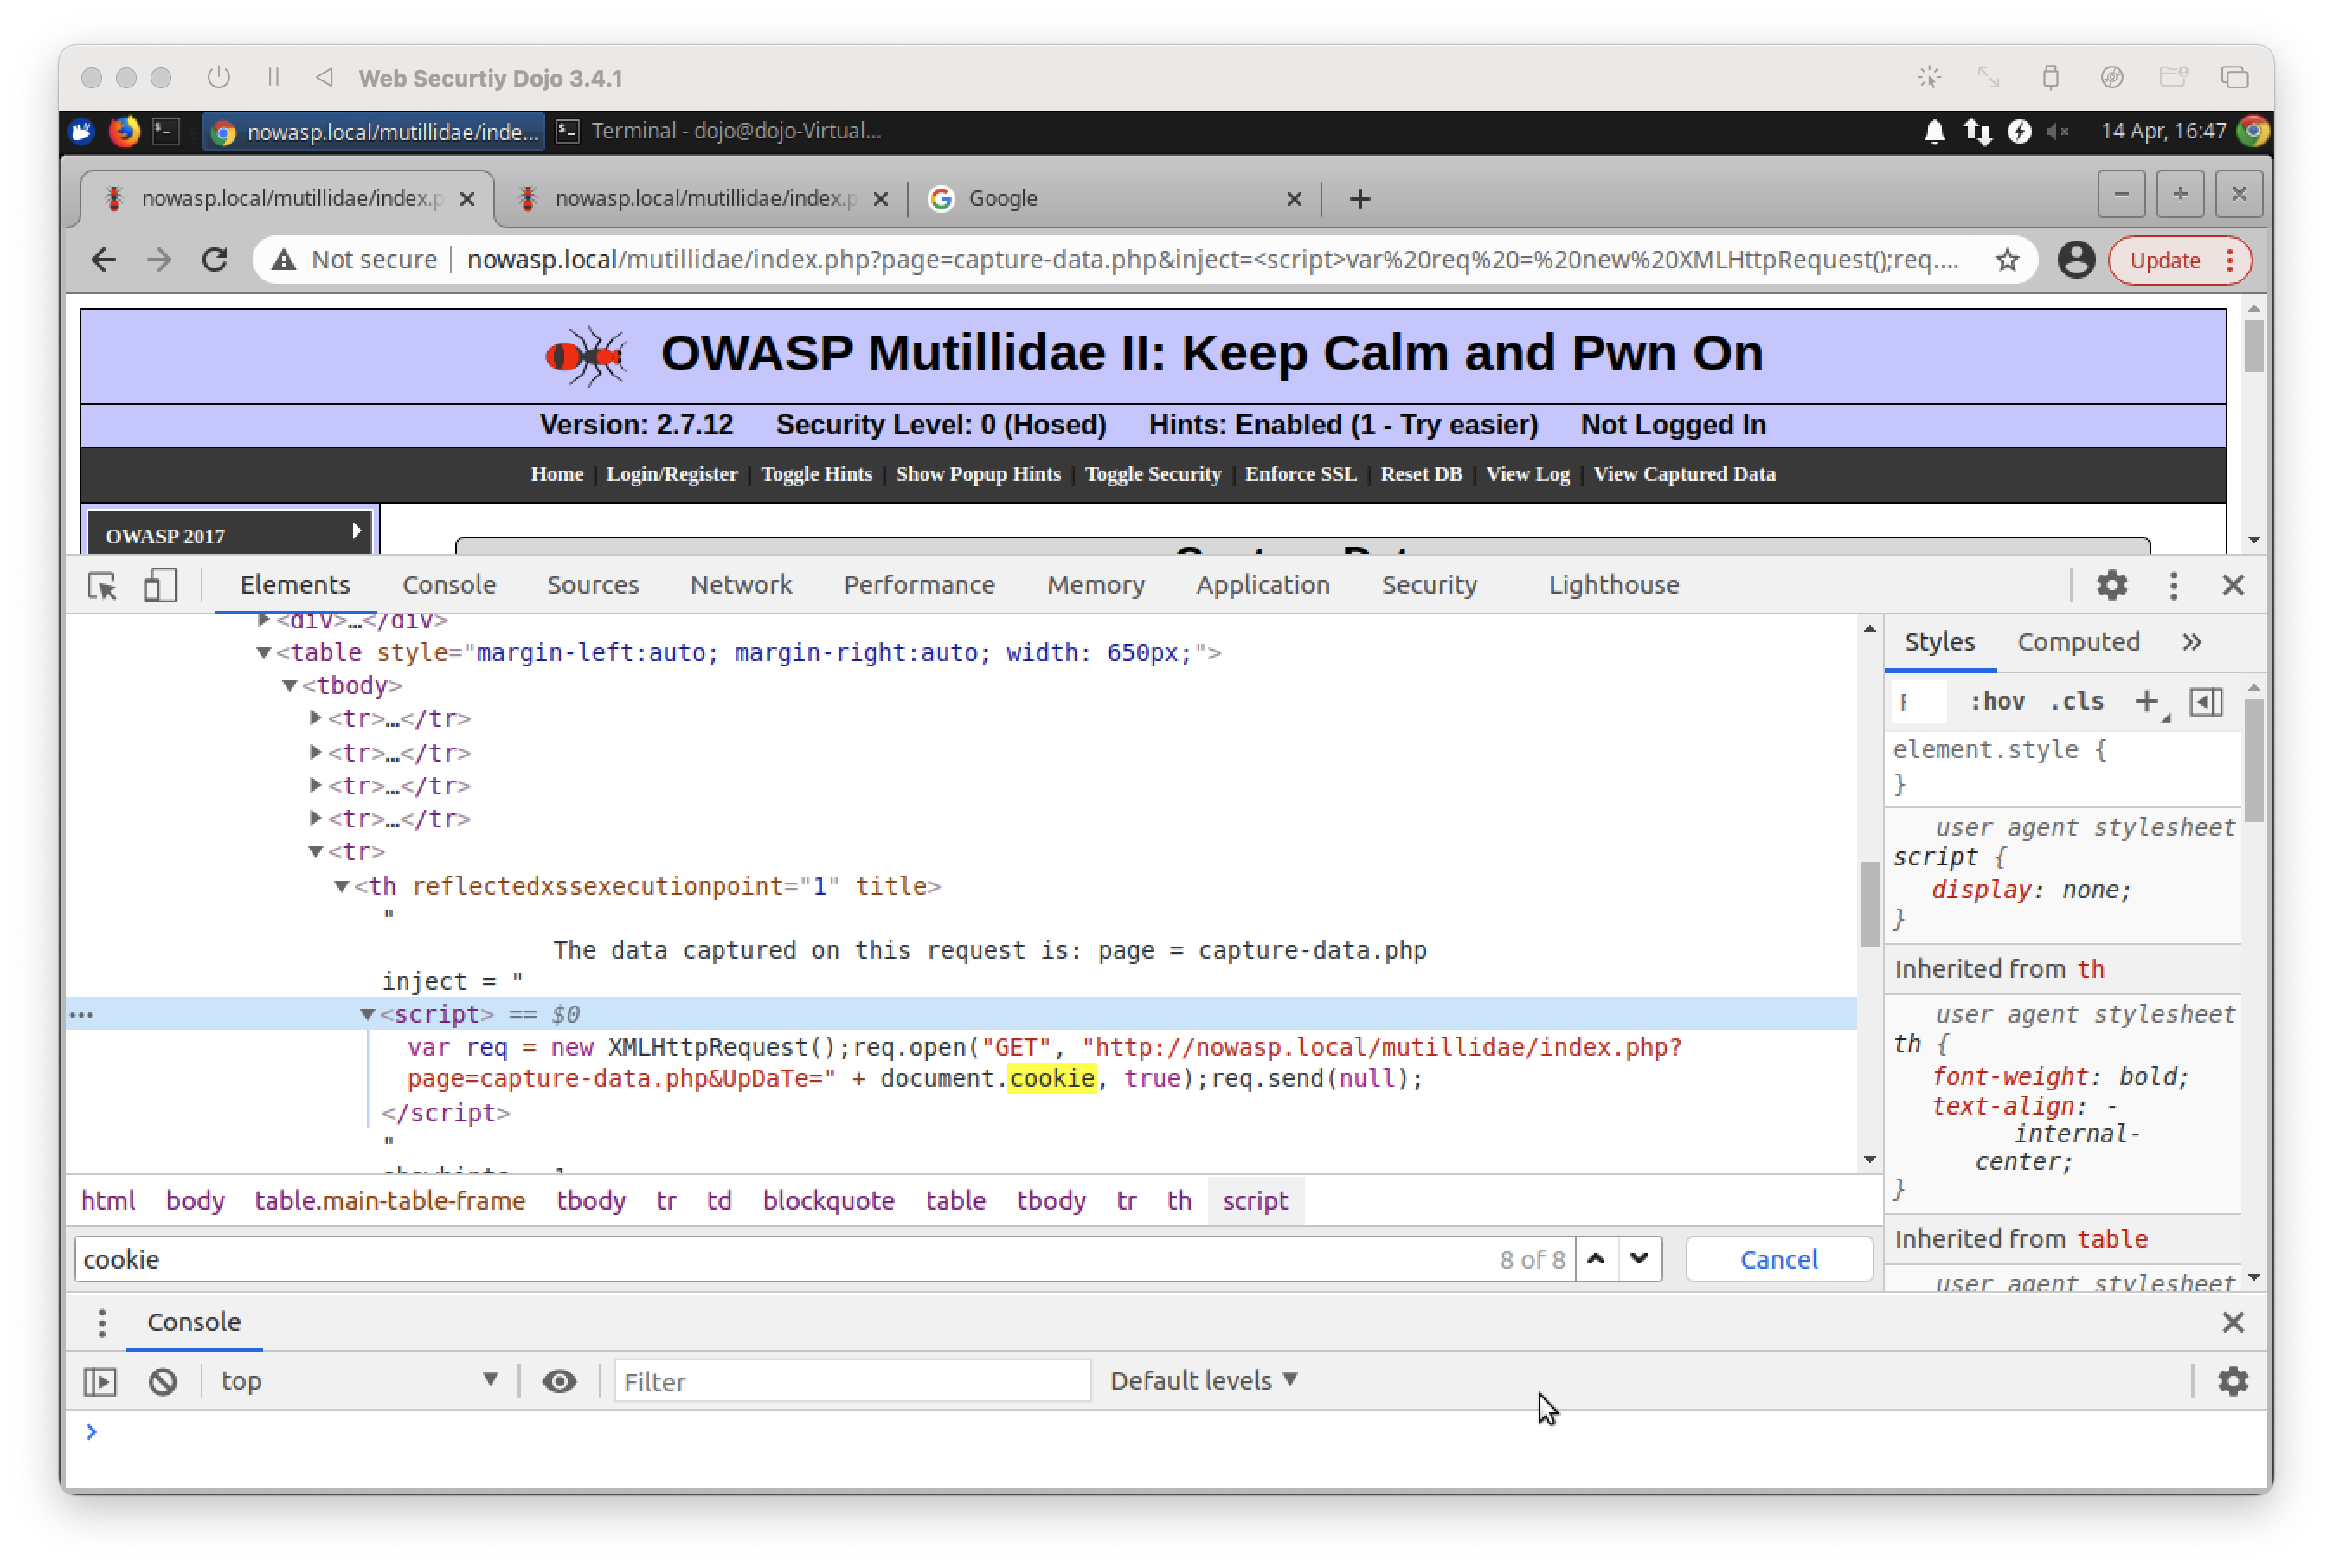
\includegraphics[width=0.8\textwidth]{step_00030}
    \caption{Теперь код злоумышленника встроен верно}
  \end{figure}

  \begin{figure}[H]
    \centering
    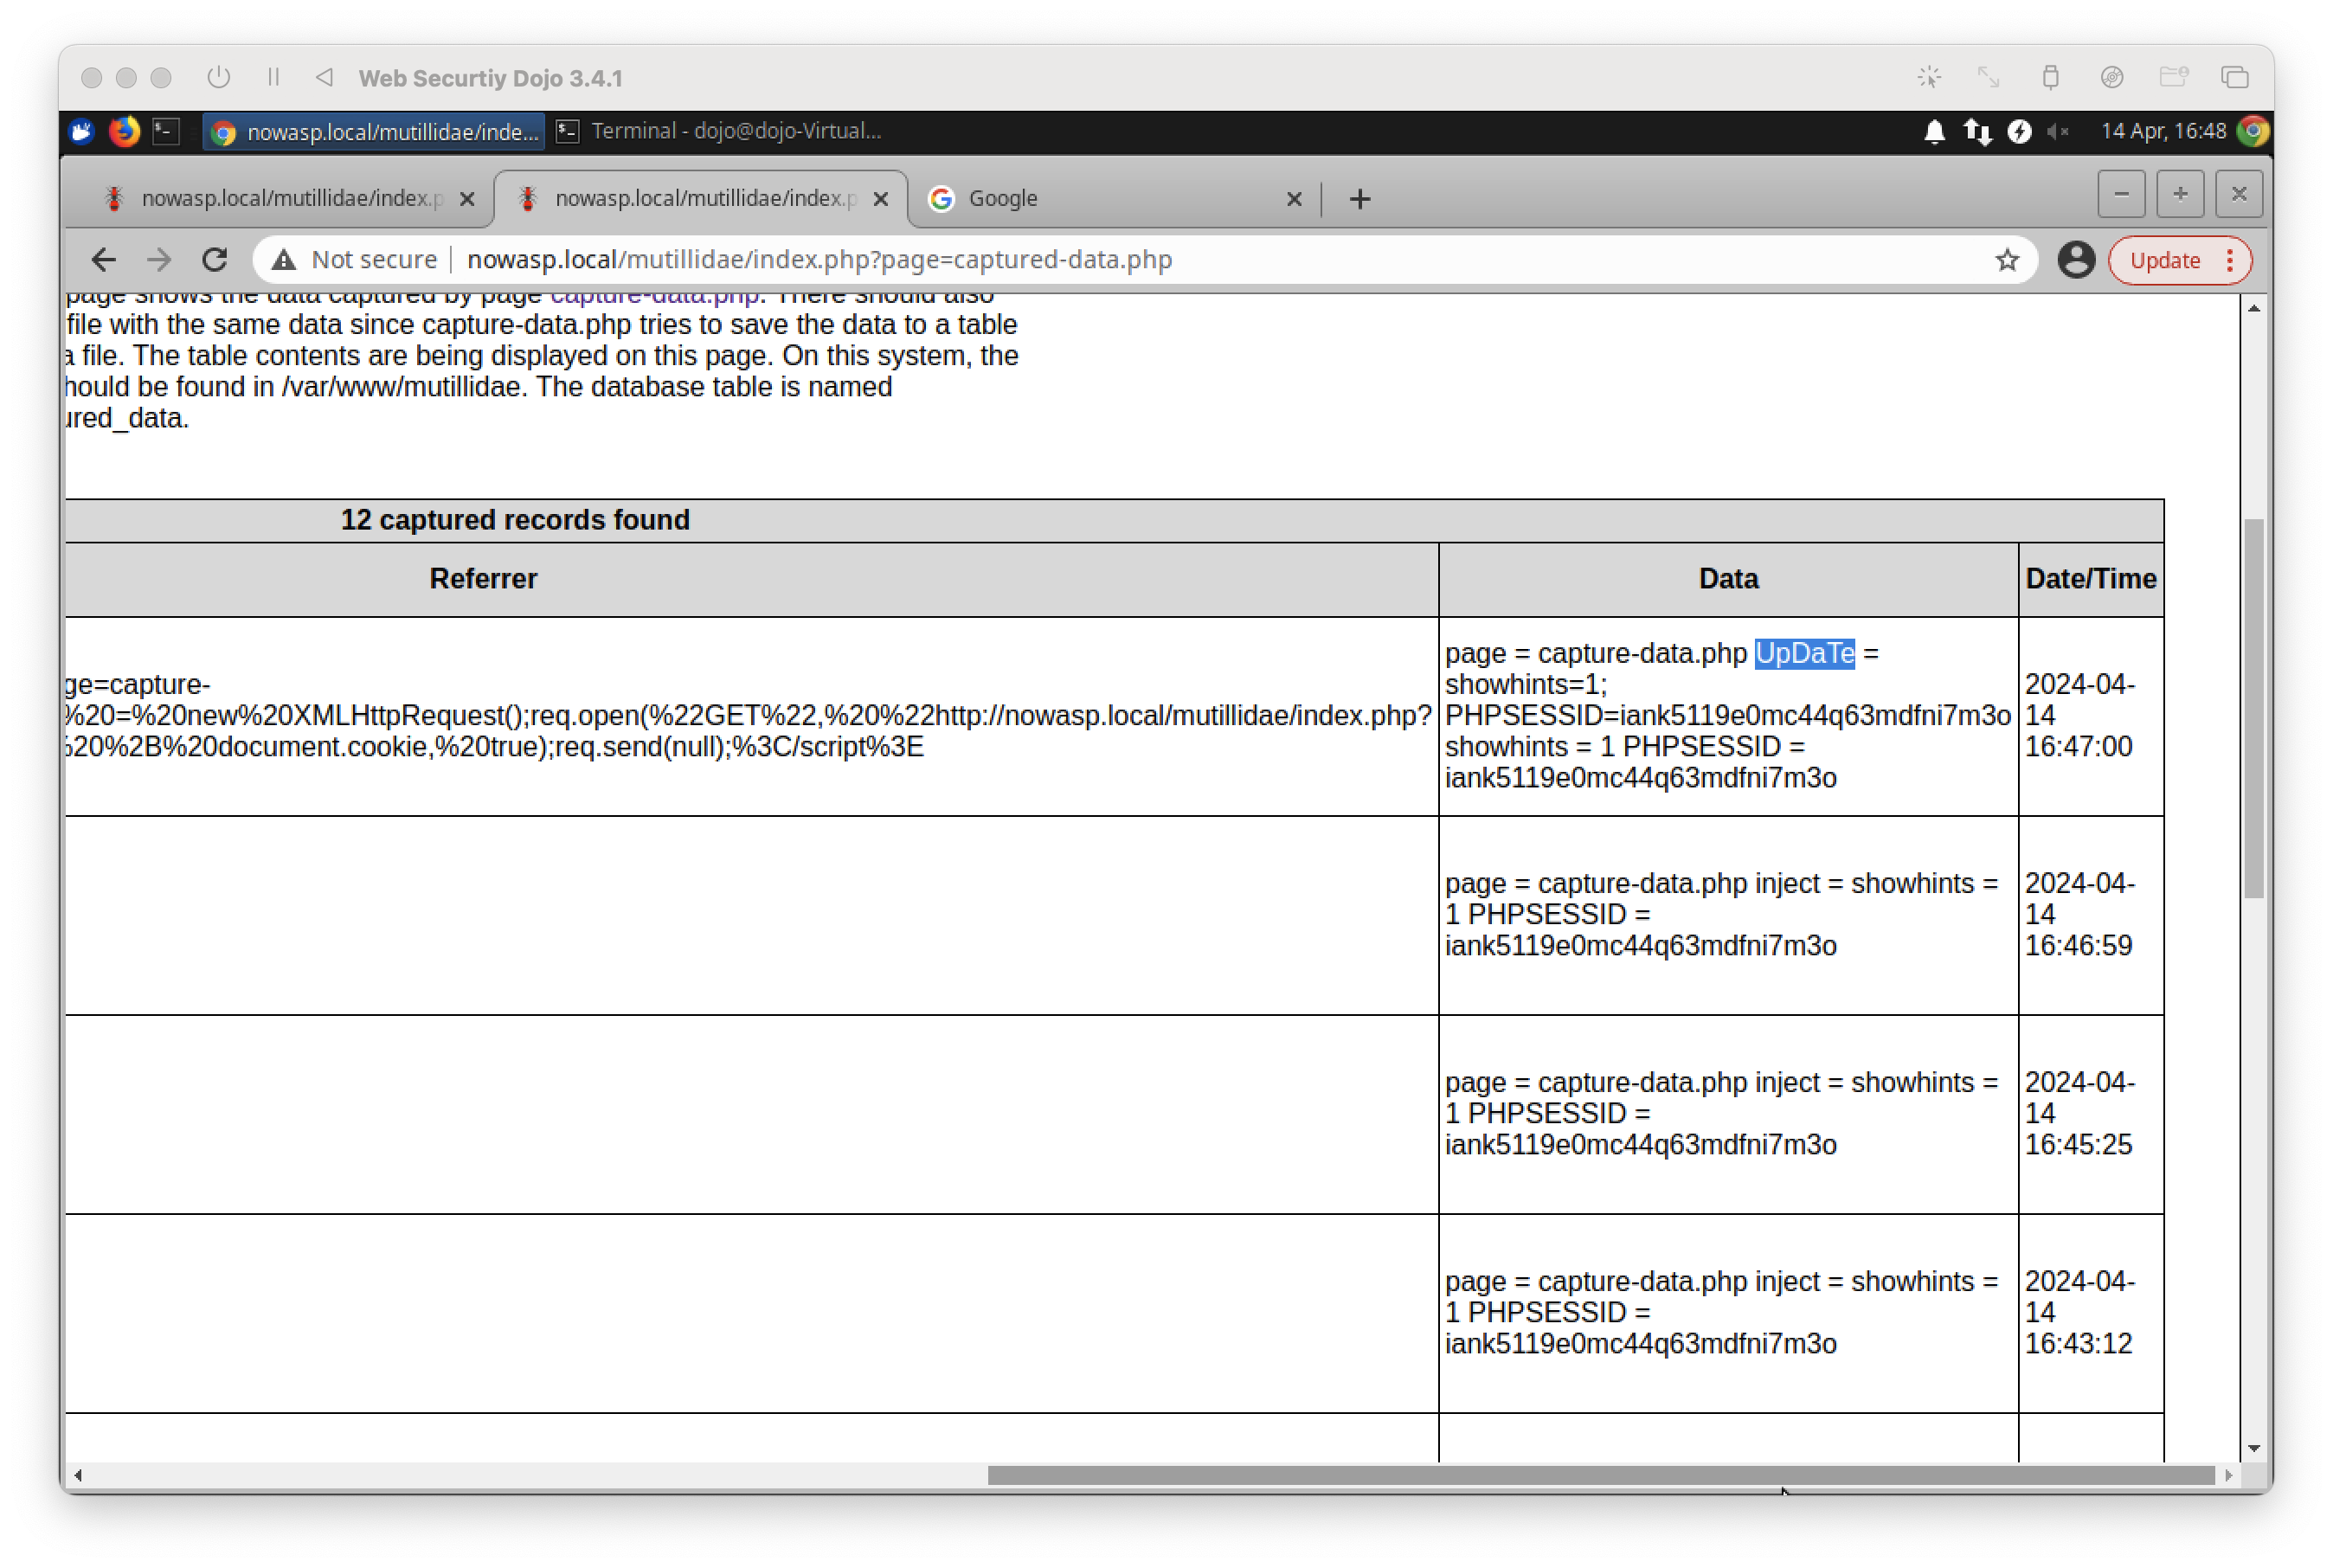
\includegraphics[width=0.8\textwidth]{step_00031}
    \caption{И по истории видим, что он отработал}
  \end{figure}

  \subsection{Атака HTML 5 Web Storage}

  \begin{figure}[H]
    \centering
    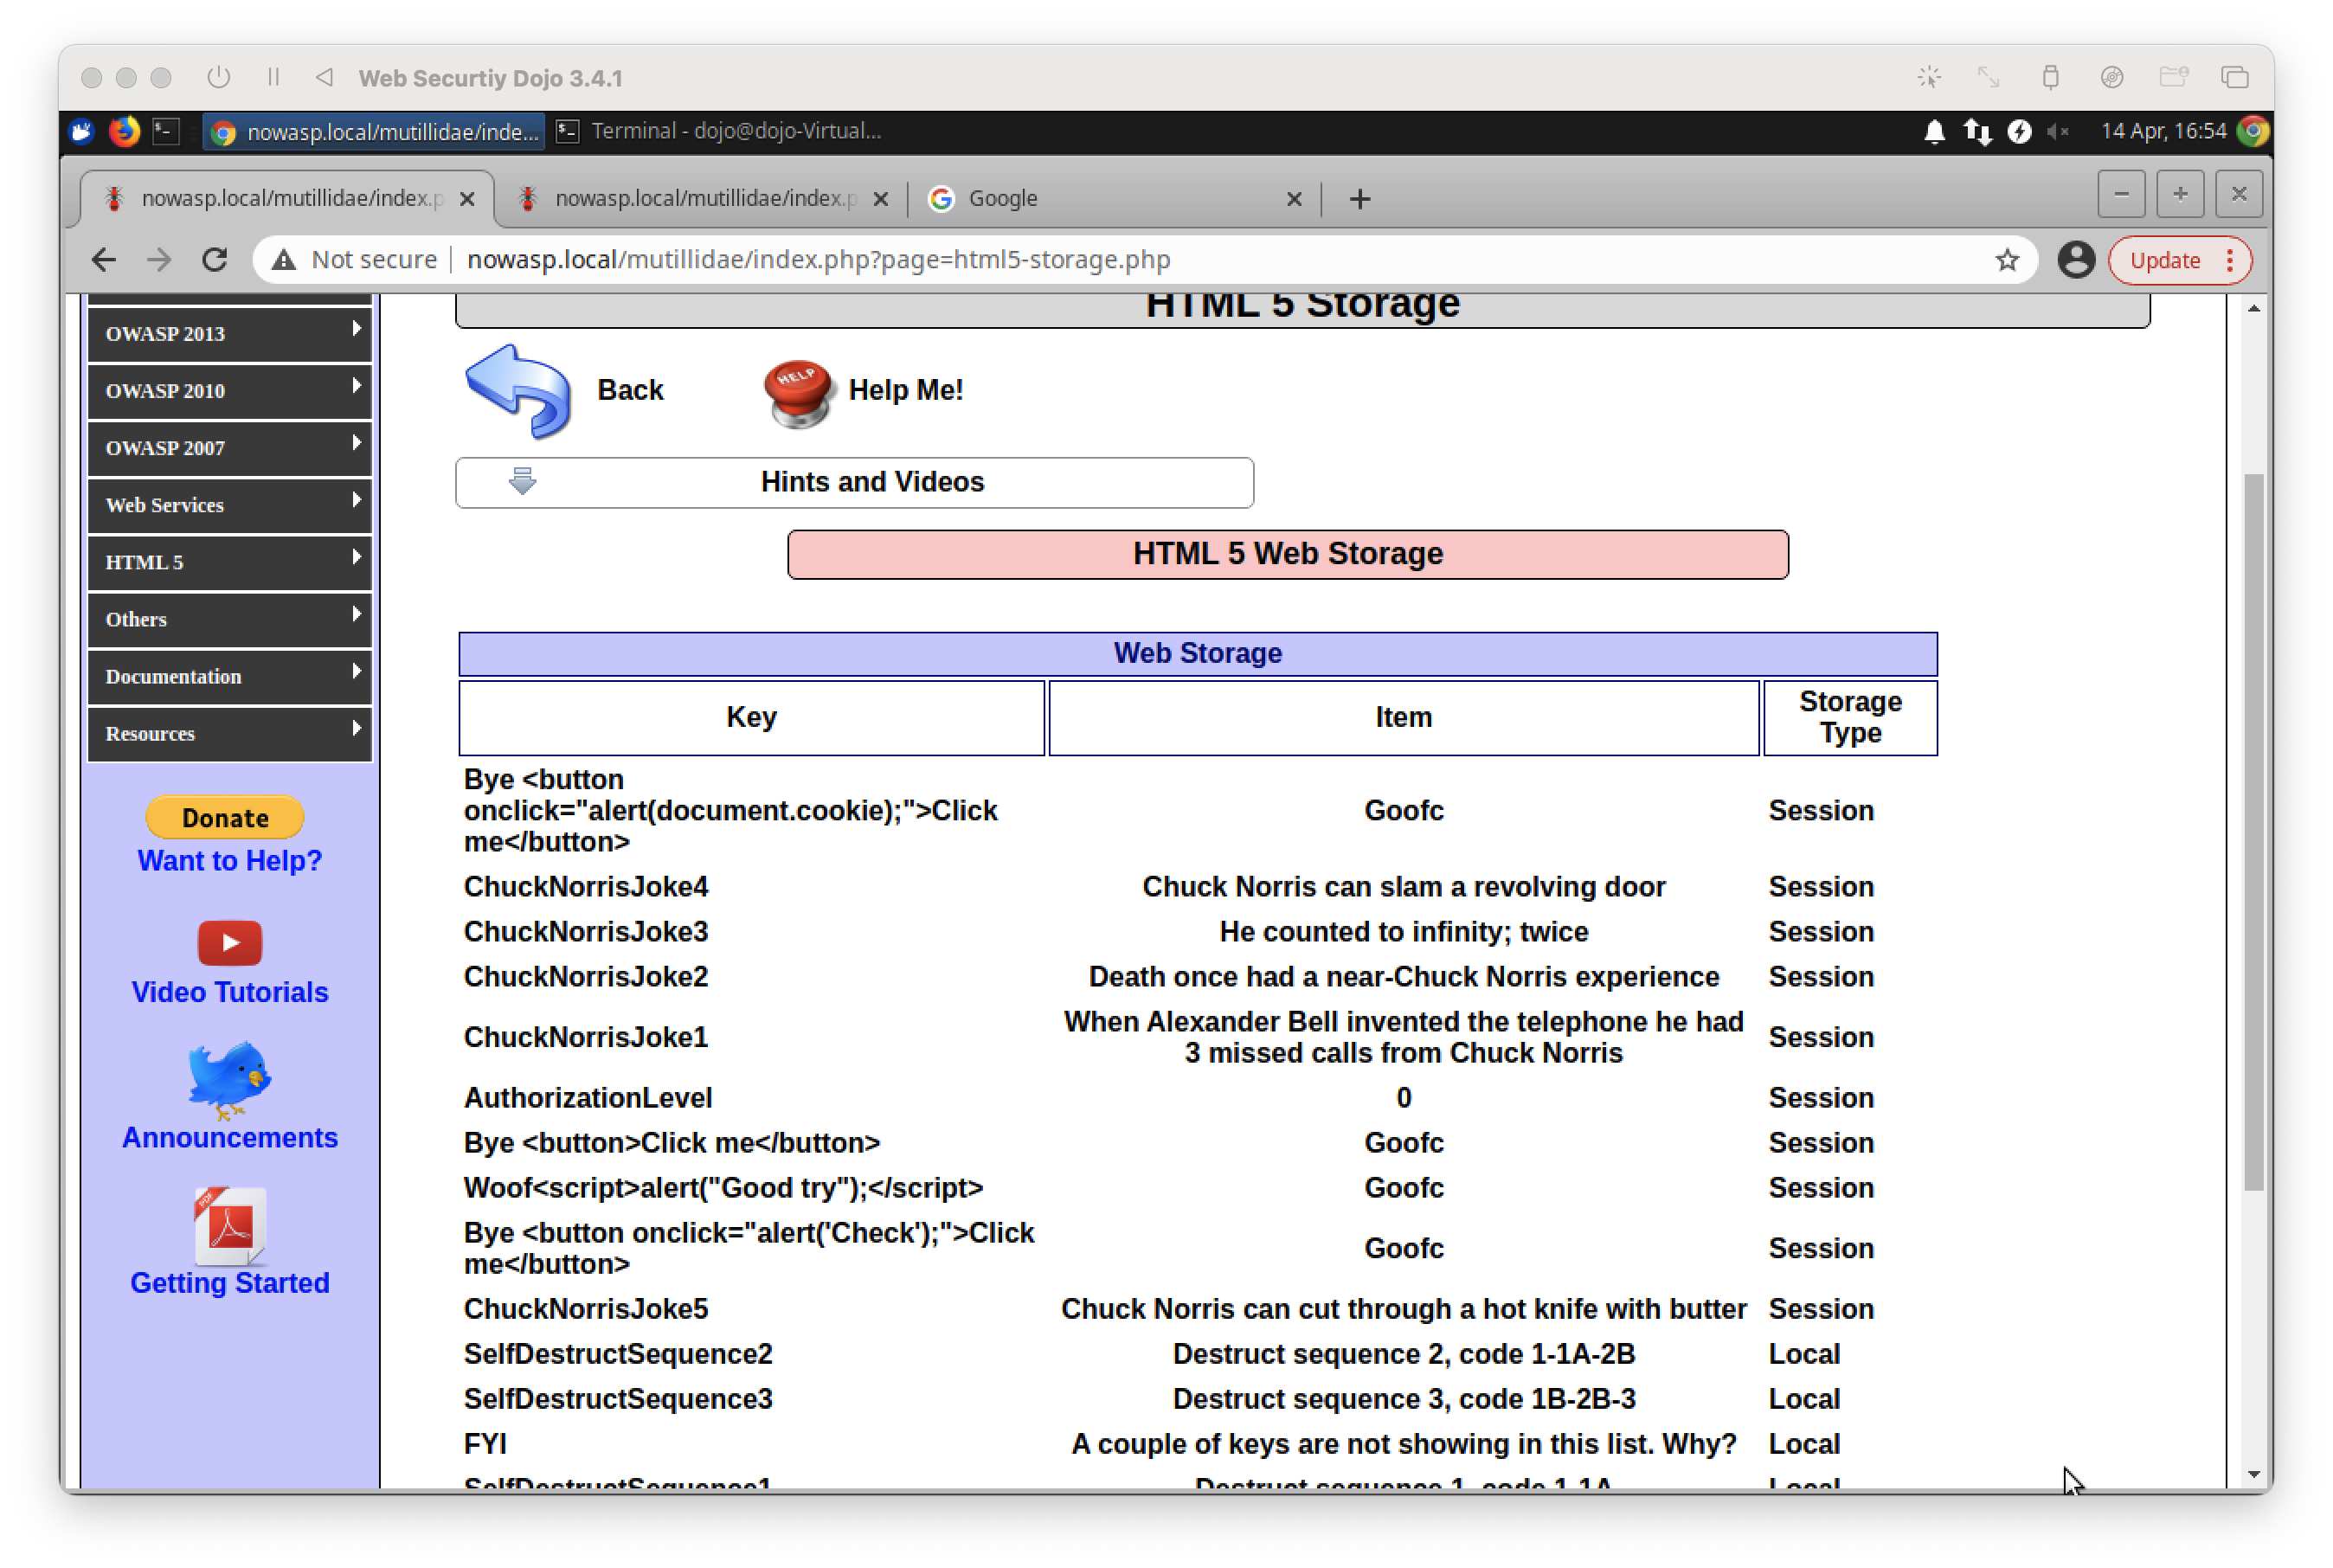
\includegraphics[width=0.8\textwidth]{step_00032}
    \caption{Рассмотрим страницу для атаки}
  \end{figure}

  \begin{figure}[H]
    \centering
    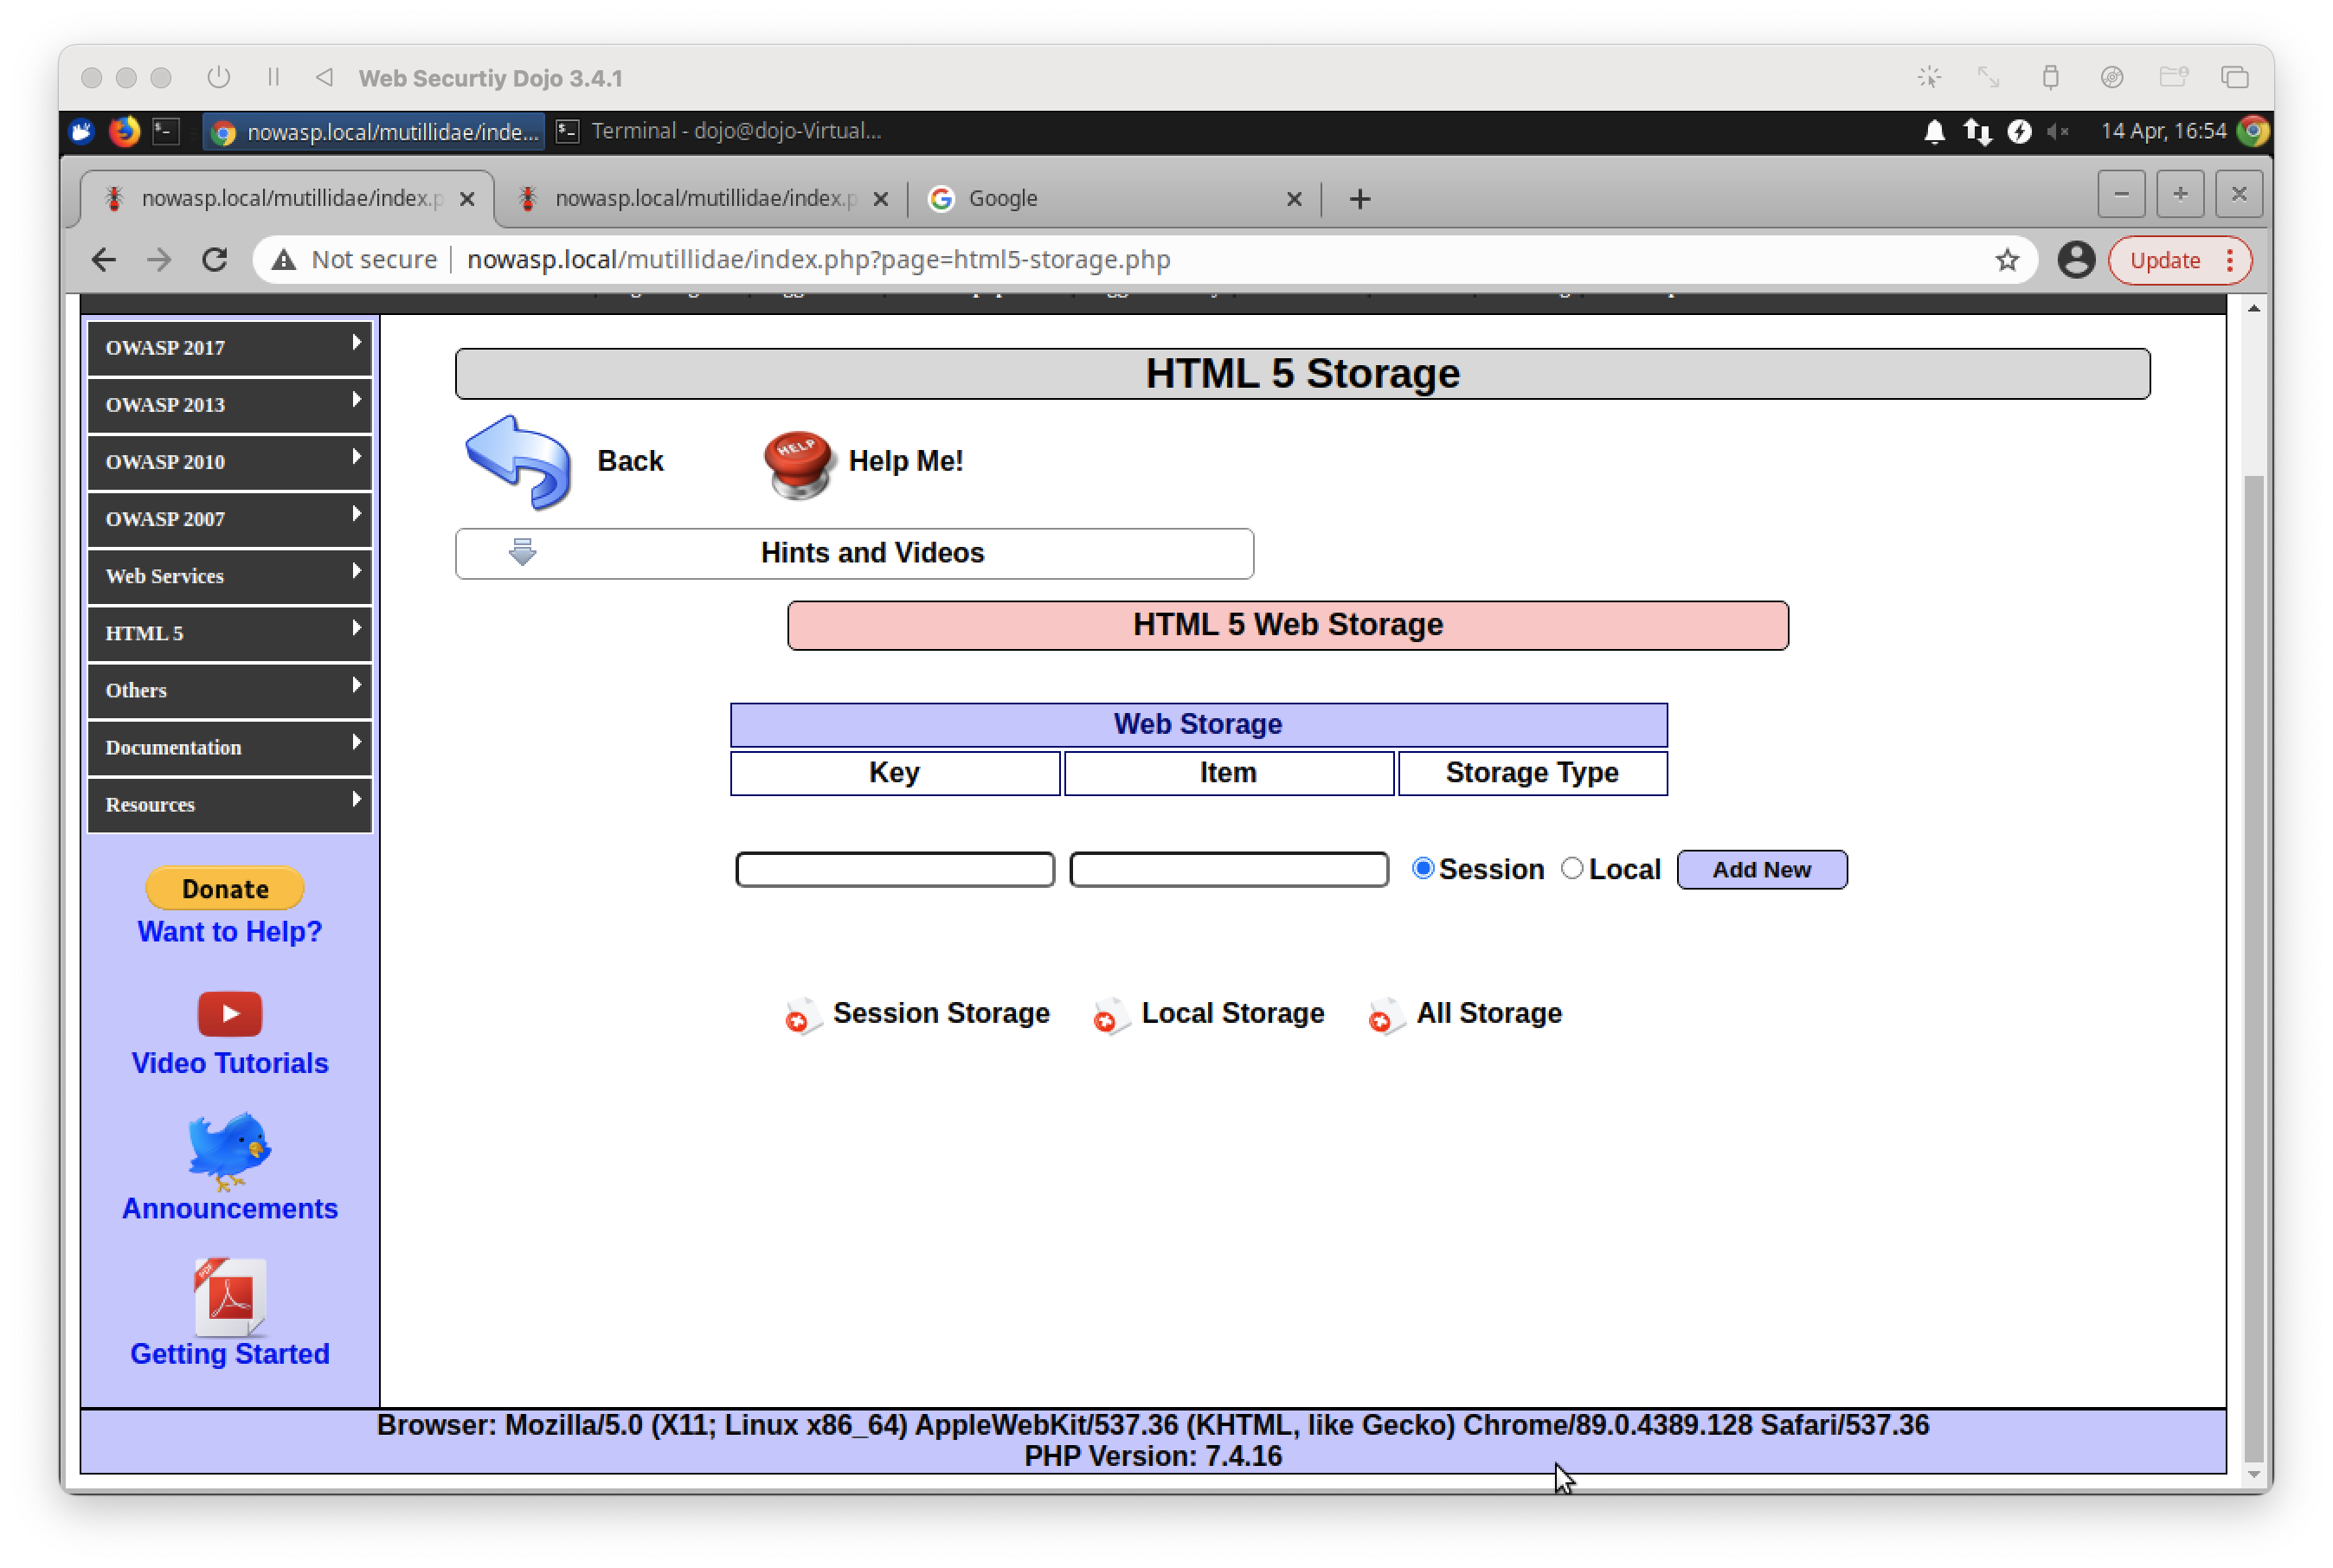
\includegraphics[width=0.8\textwidth]{step_00033}
    \caption{Изначально почистим её, чтобы старые записи не мешали}
  \end{figure}

  \begin{figure}[H]
    \centering
    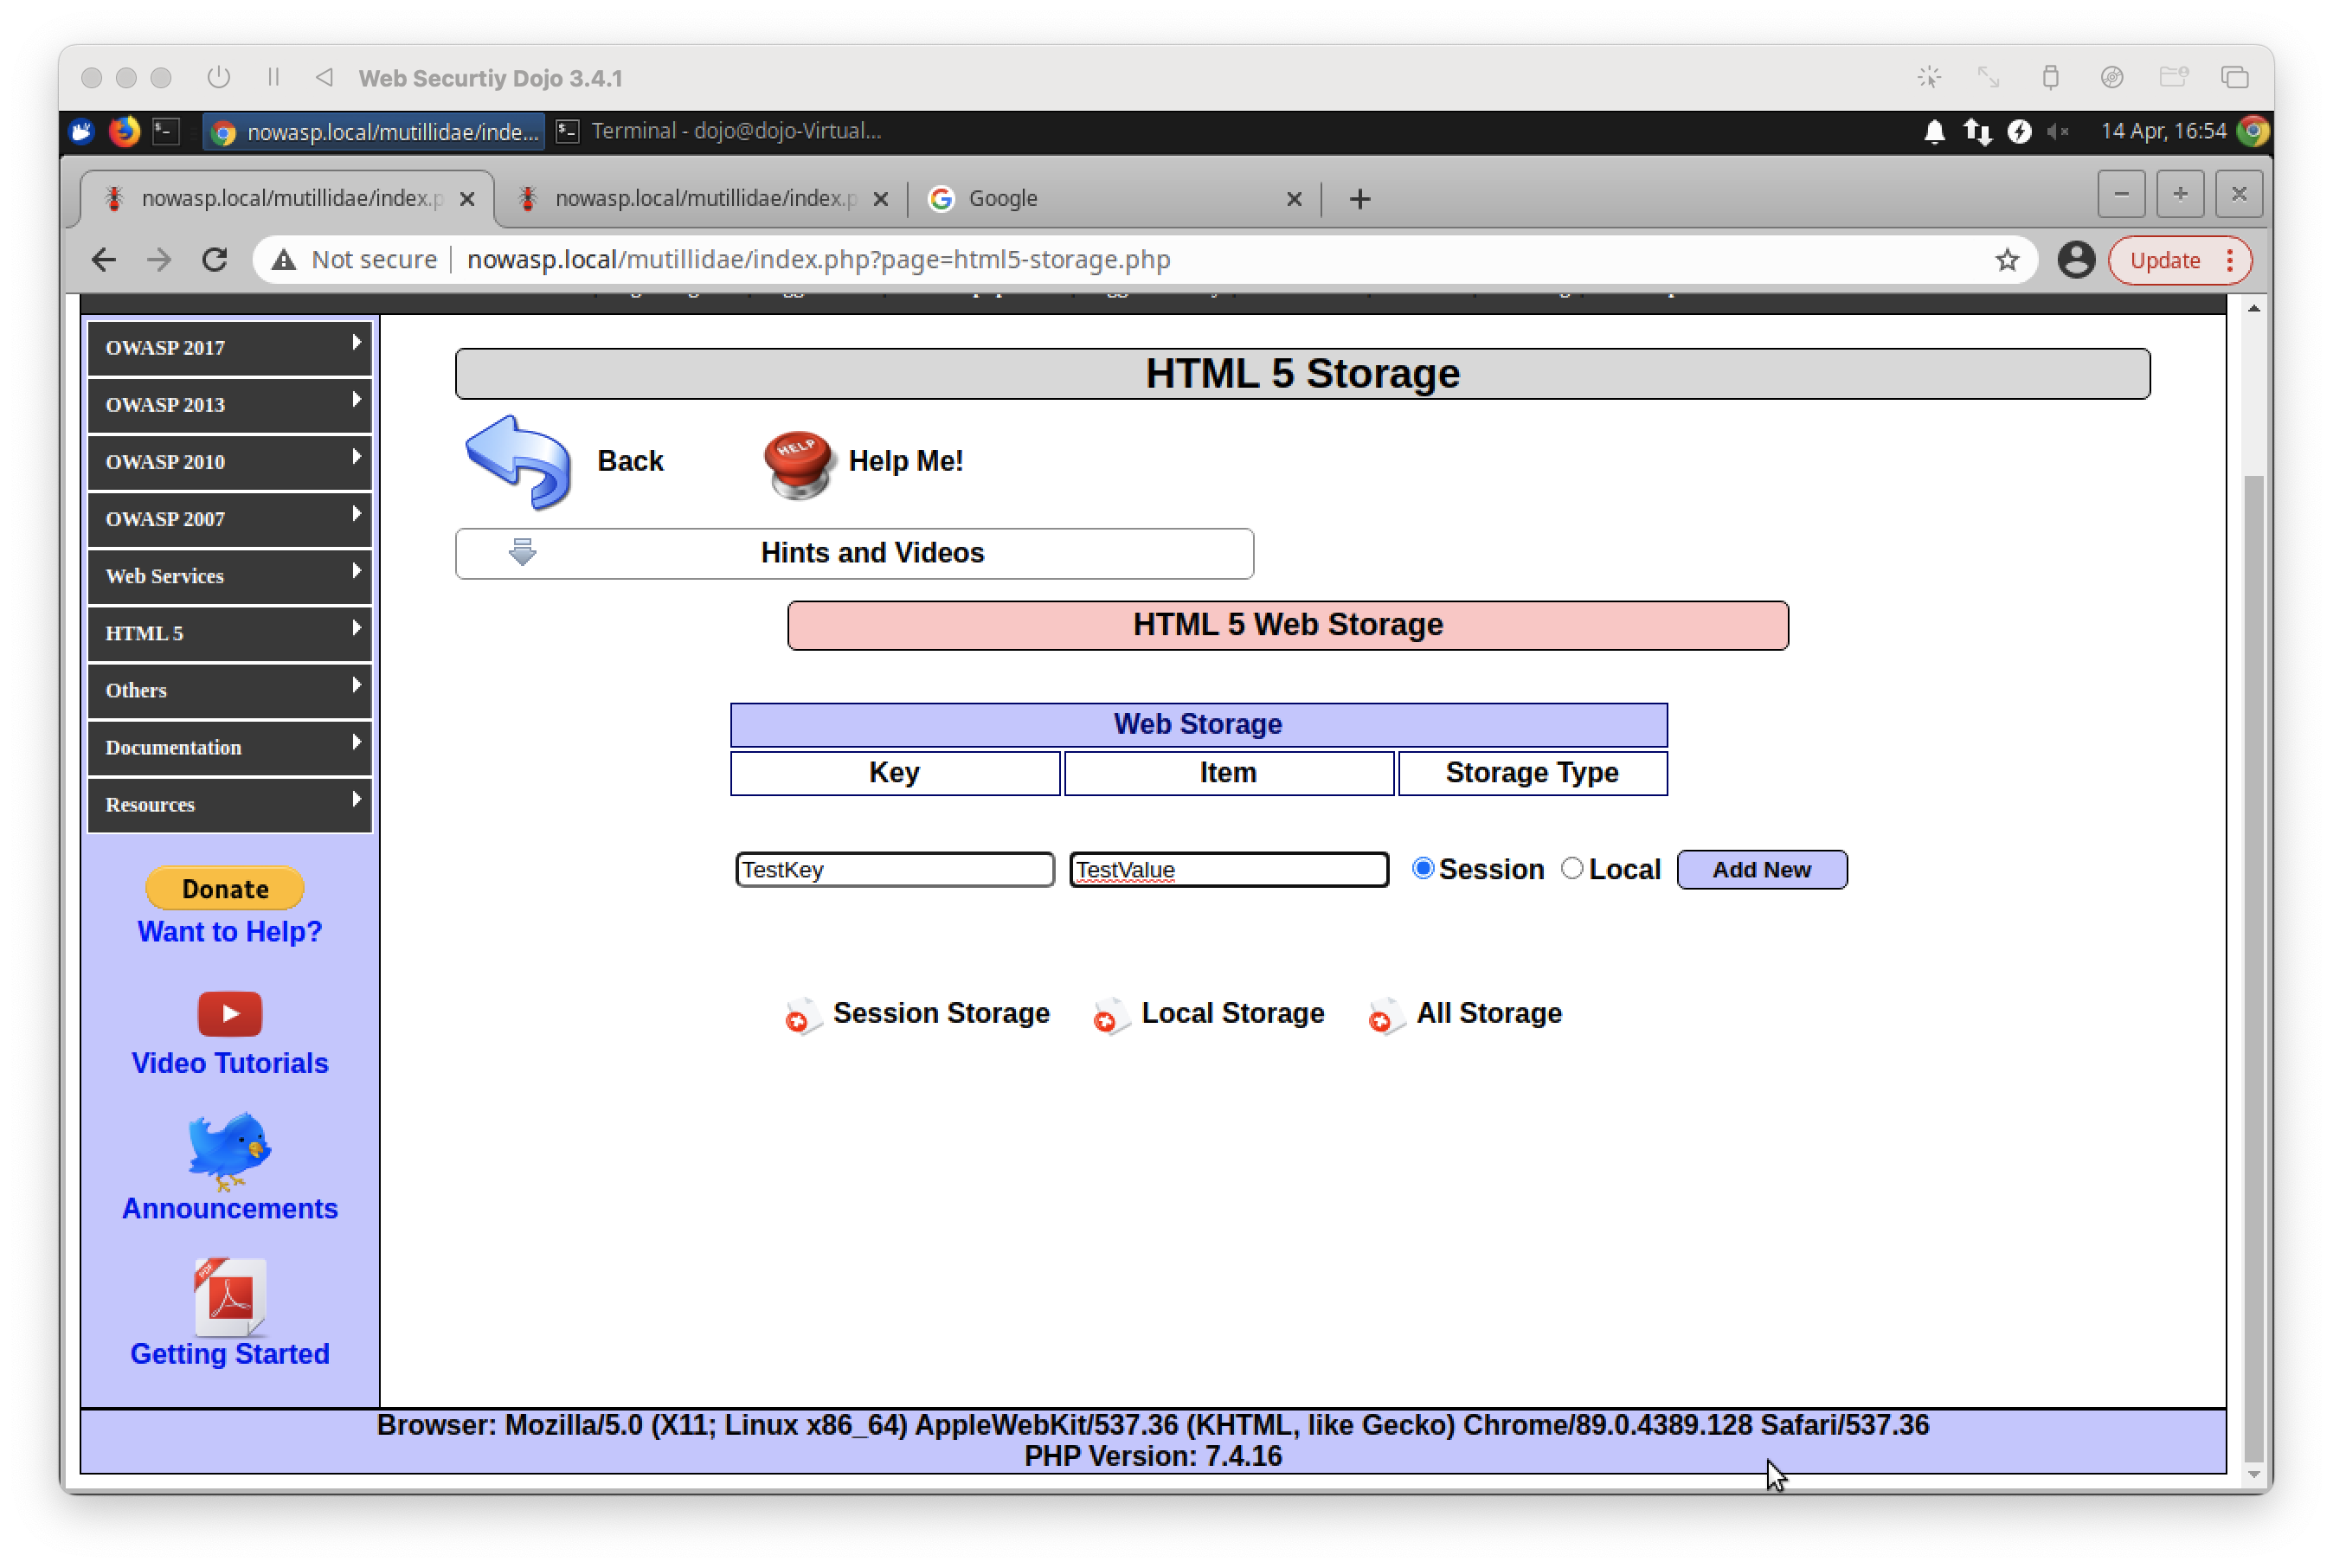
\includegraphics[width=0.8\textwidth]{step_00034}
    \caption{Пробуем добавить обычную запись}
  \end{figure}

  \begin{figure}[H]
    \centering
    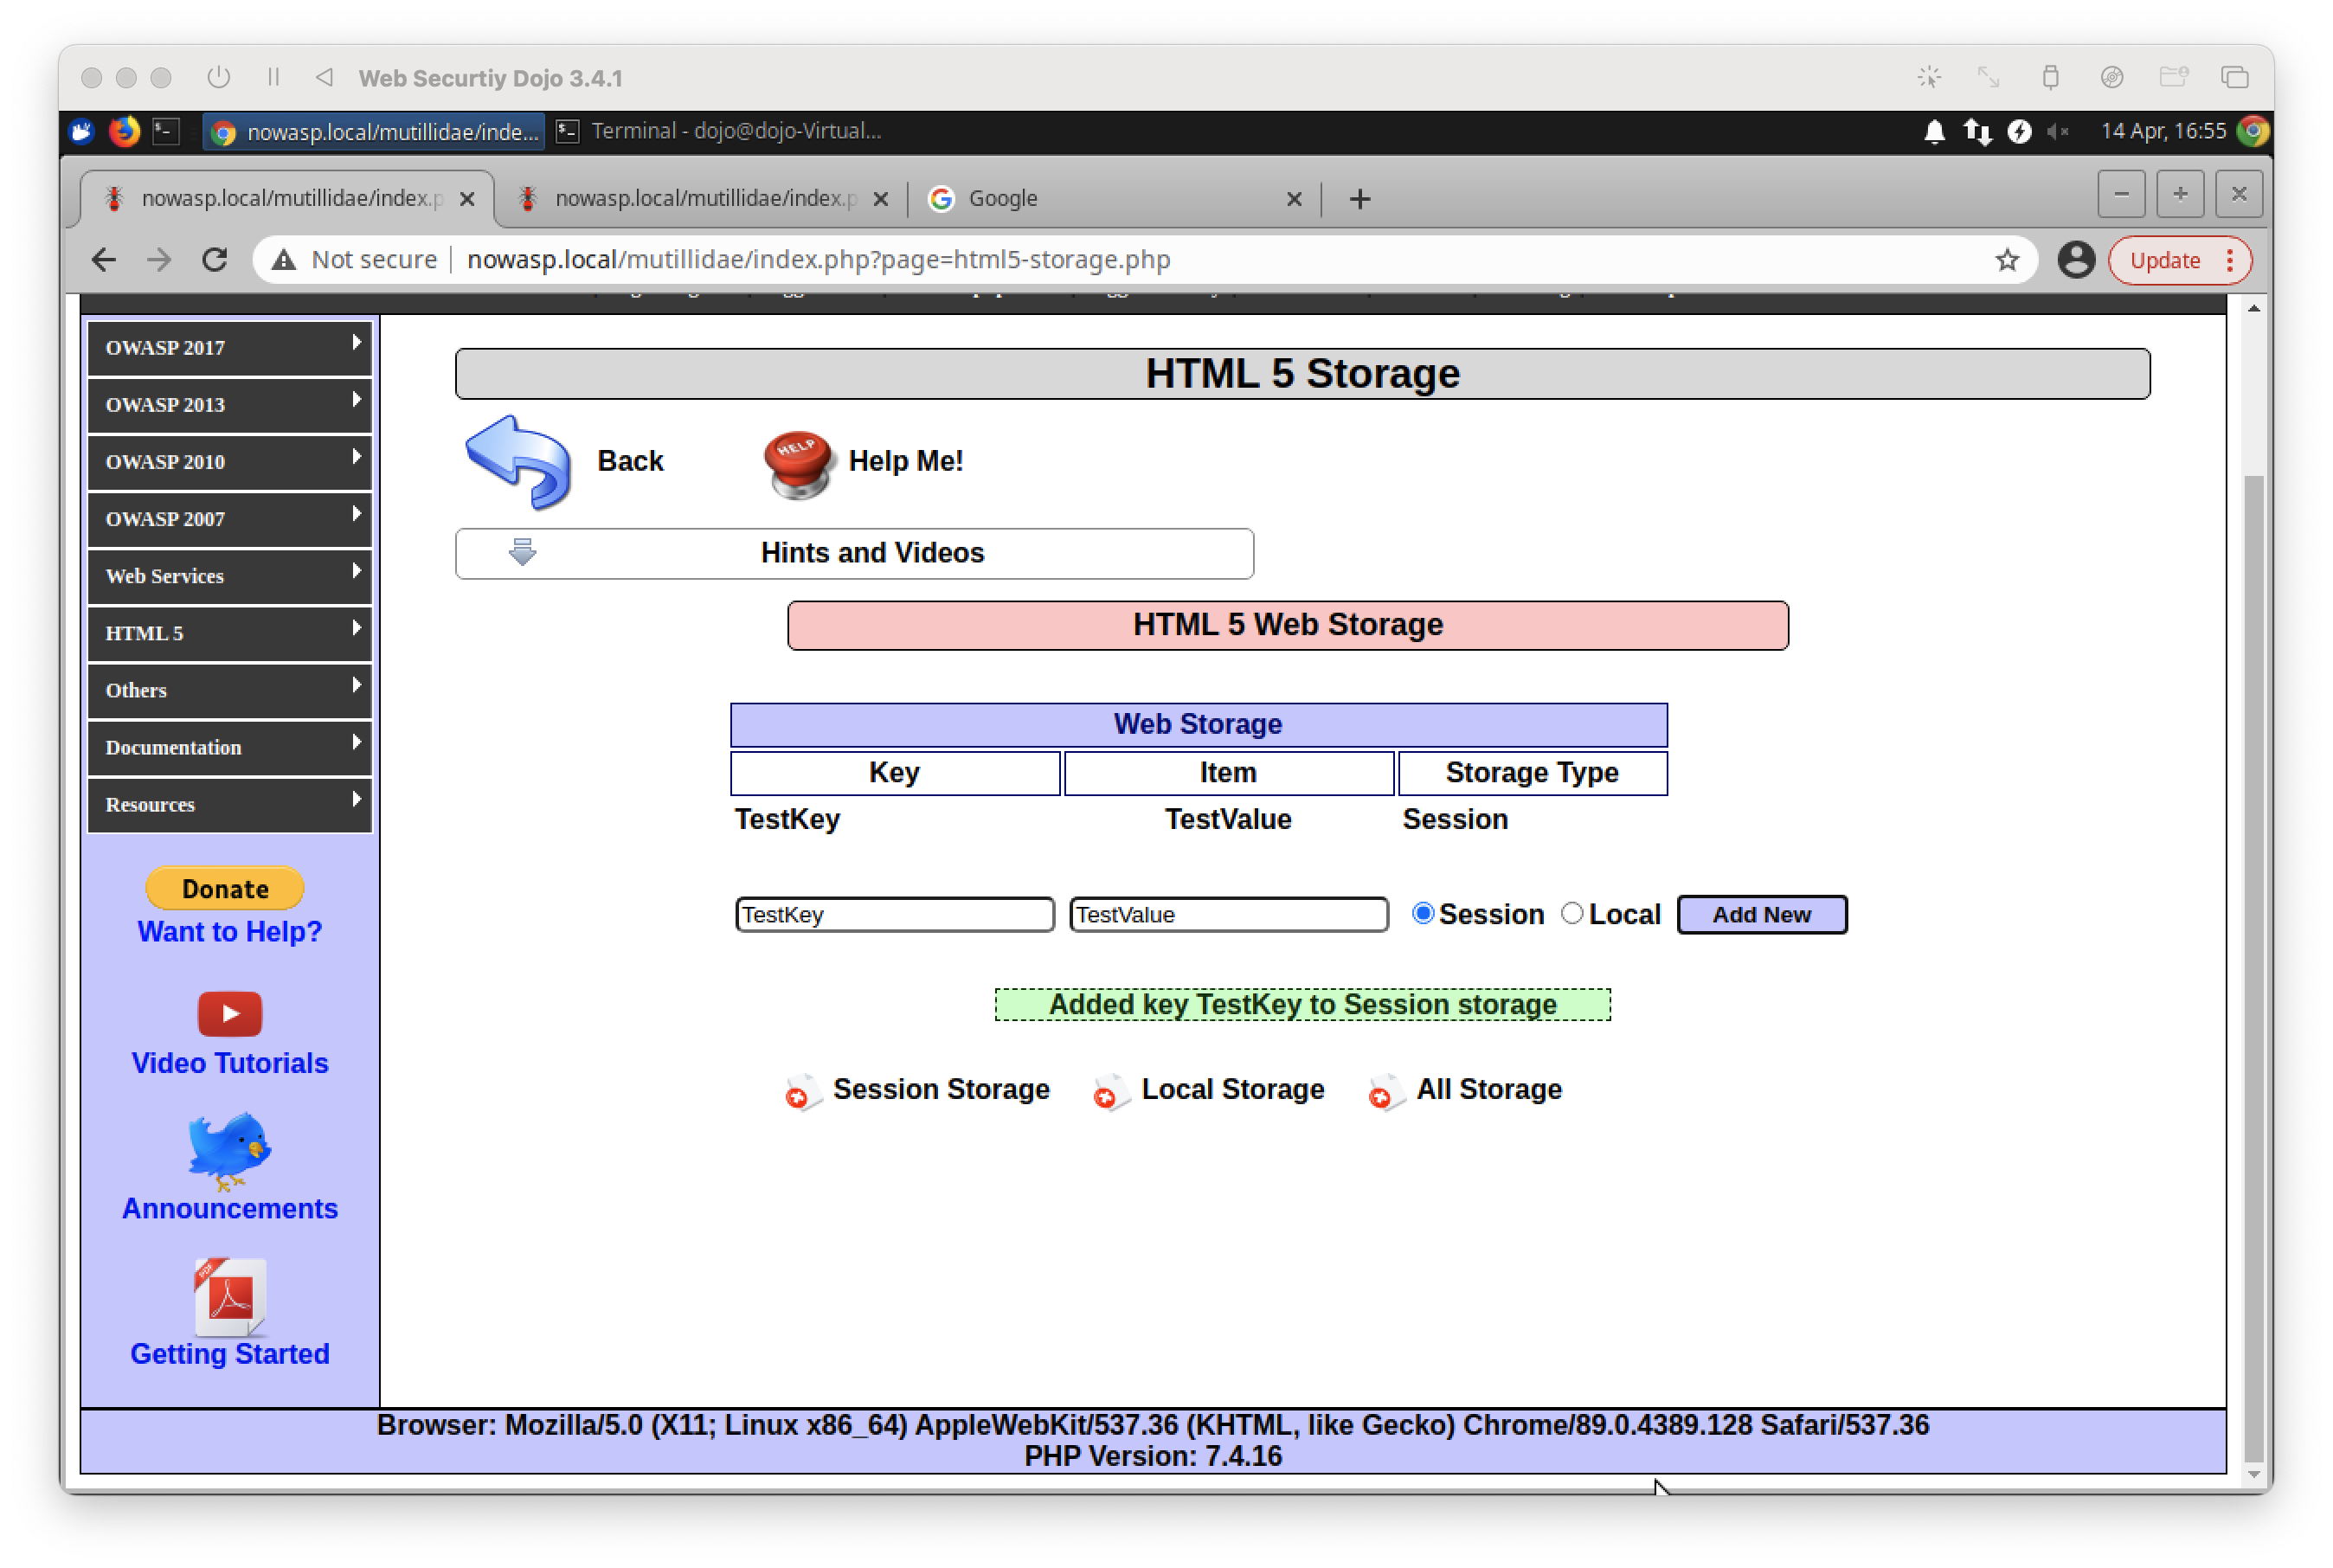
\includegraphics[width=0.8\textwidth]{step_00035}
    \caption{Всё просто работает}
  \end{figure}

  \begin{figure}[H]
    \centering
    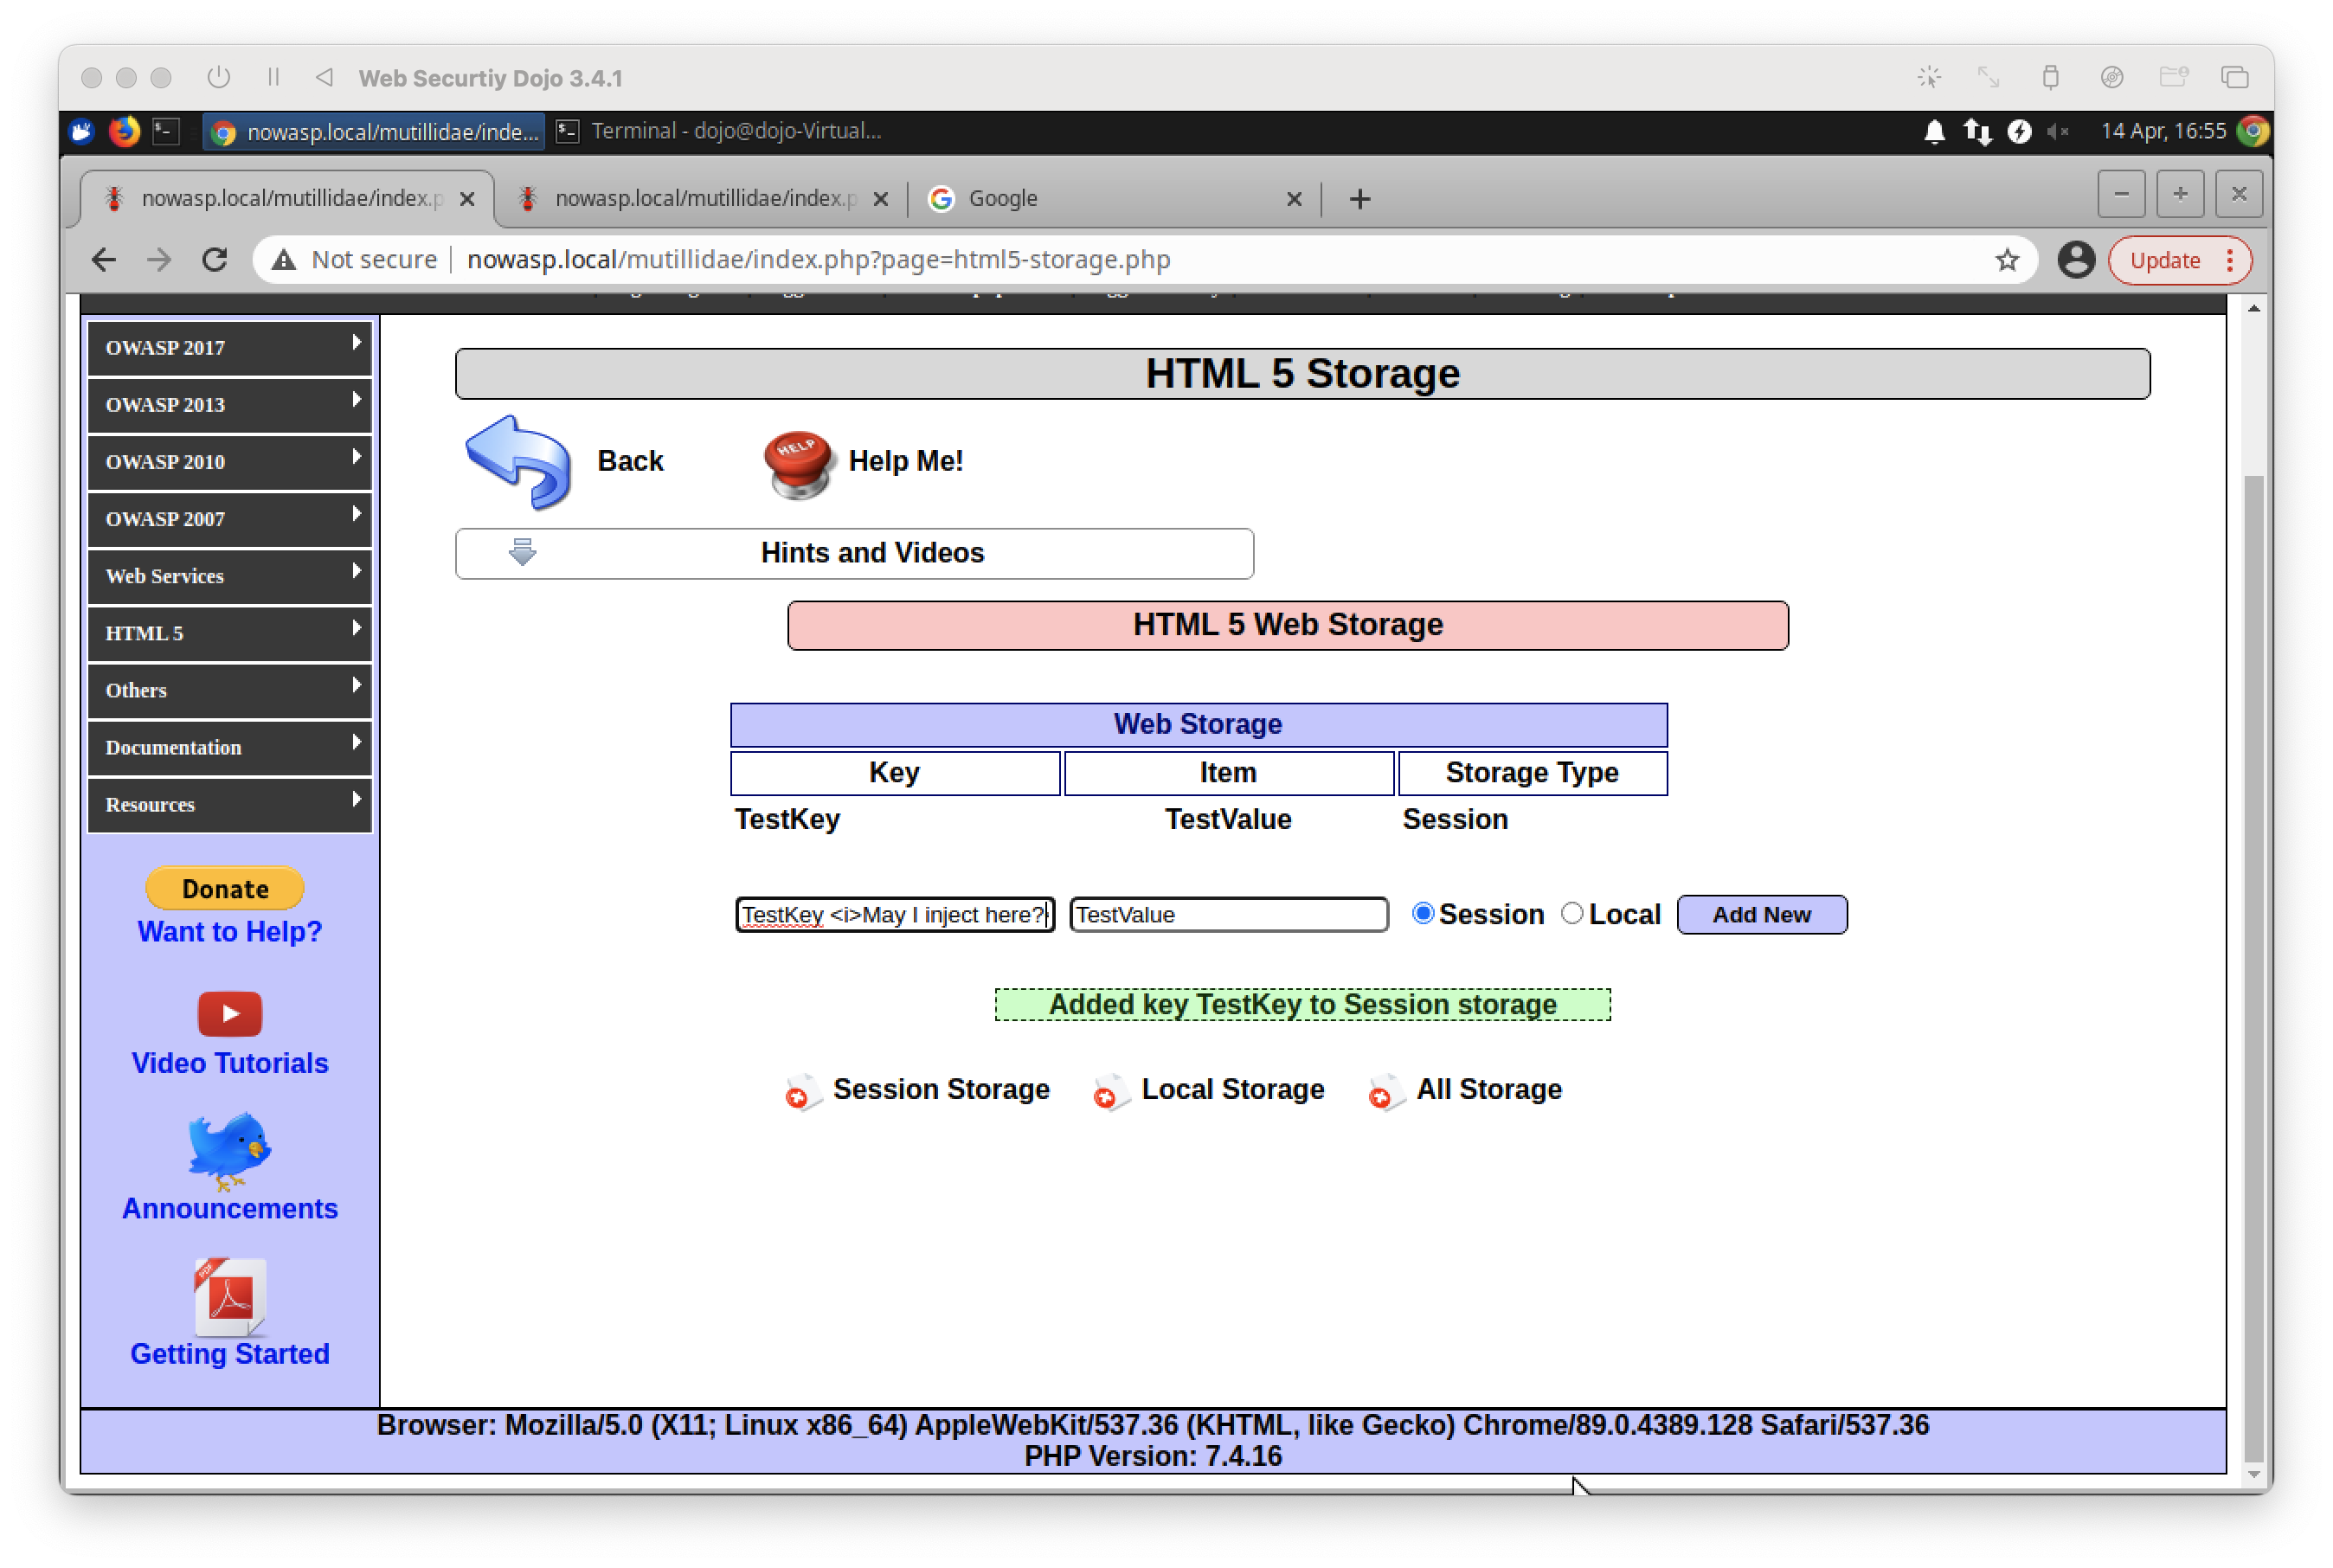
\includegraphics[width=0.8\textwidth]{step_00036}
    \caption{Пробуем встроить JS в ключ}
  \end{figure}

  \begin{figure}[H]
    \centering
    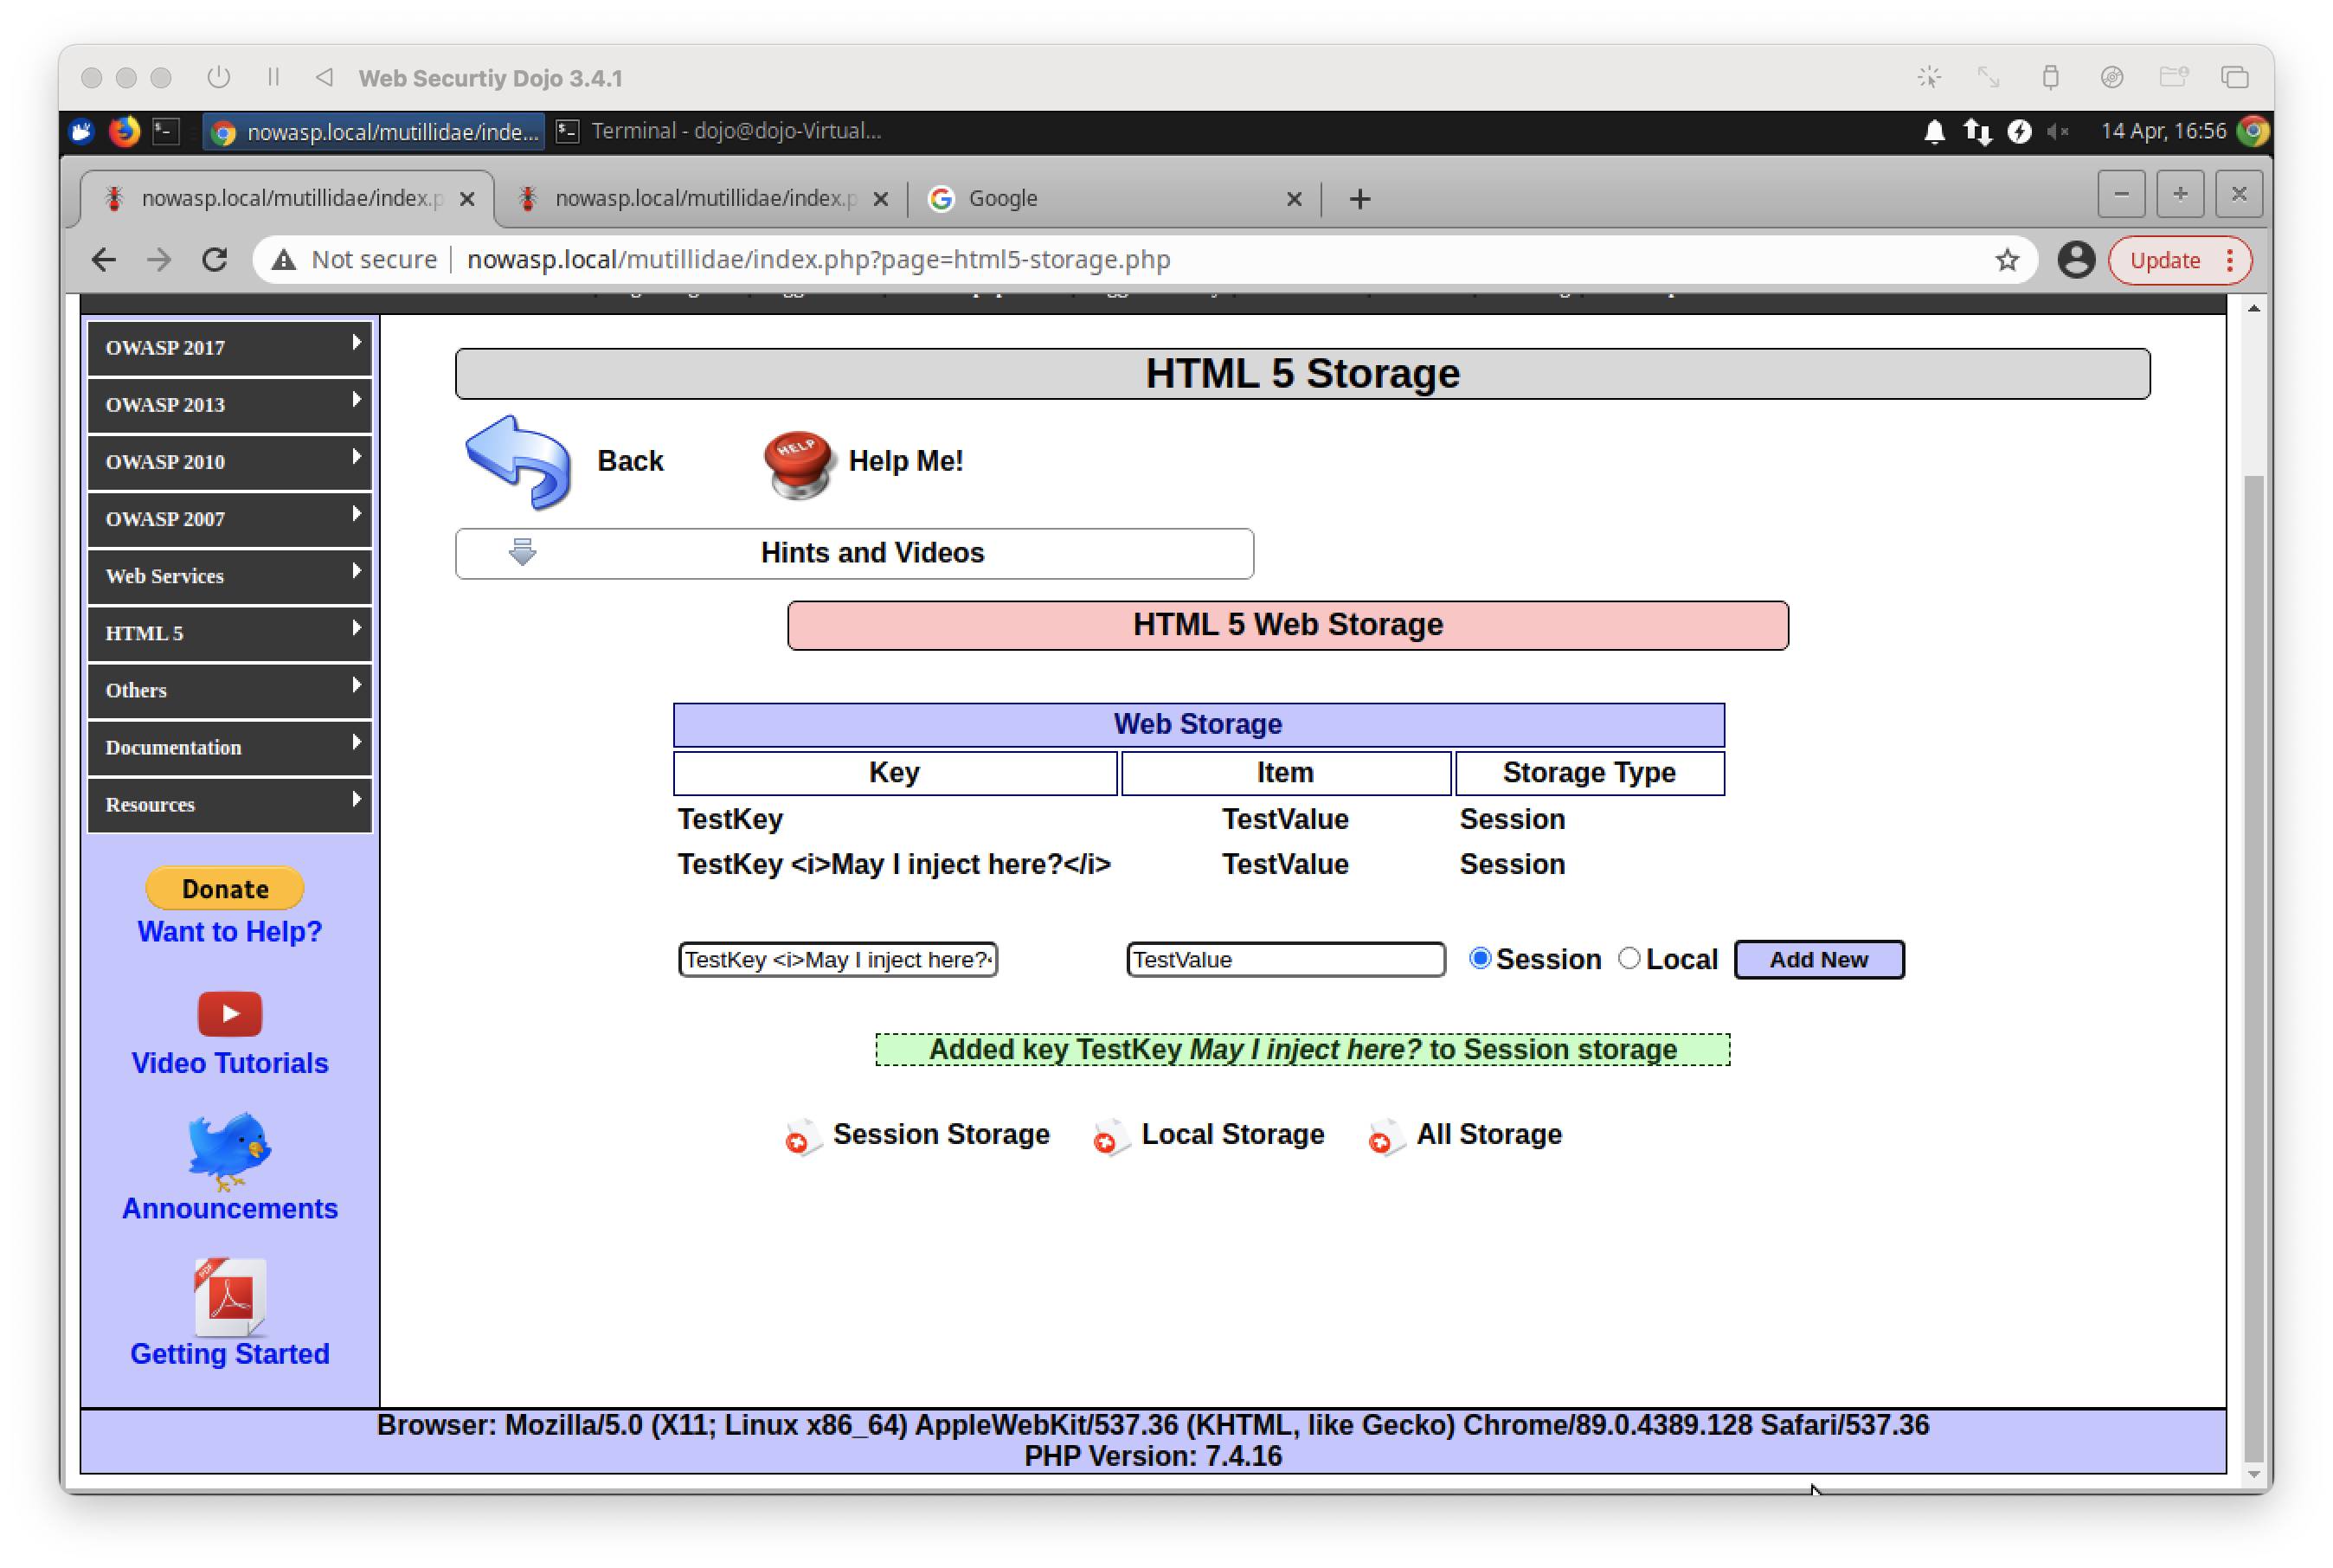
\includegraphics[width=0.8\textwidth]{step_00037}
    \caption{Почти}
  \end{figure}

  В таблице наш текст перекодировали так, что код в нём не виполнился, однако в
  тексте на зеленом фоне (уведомление об успехе) дополнительных про-верок нет.

  \begin{figure}[H]
    \centering
    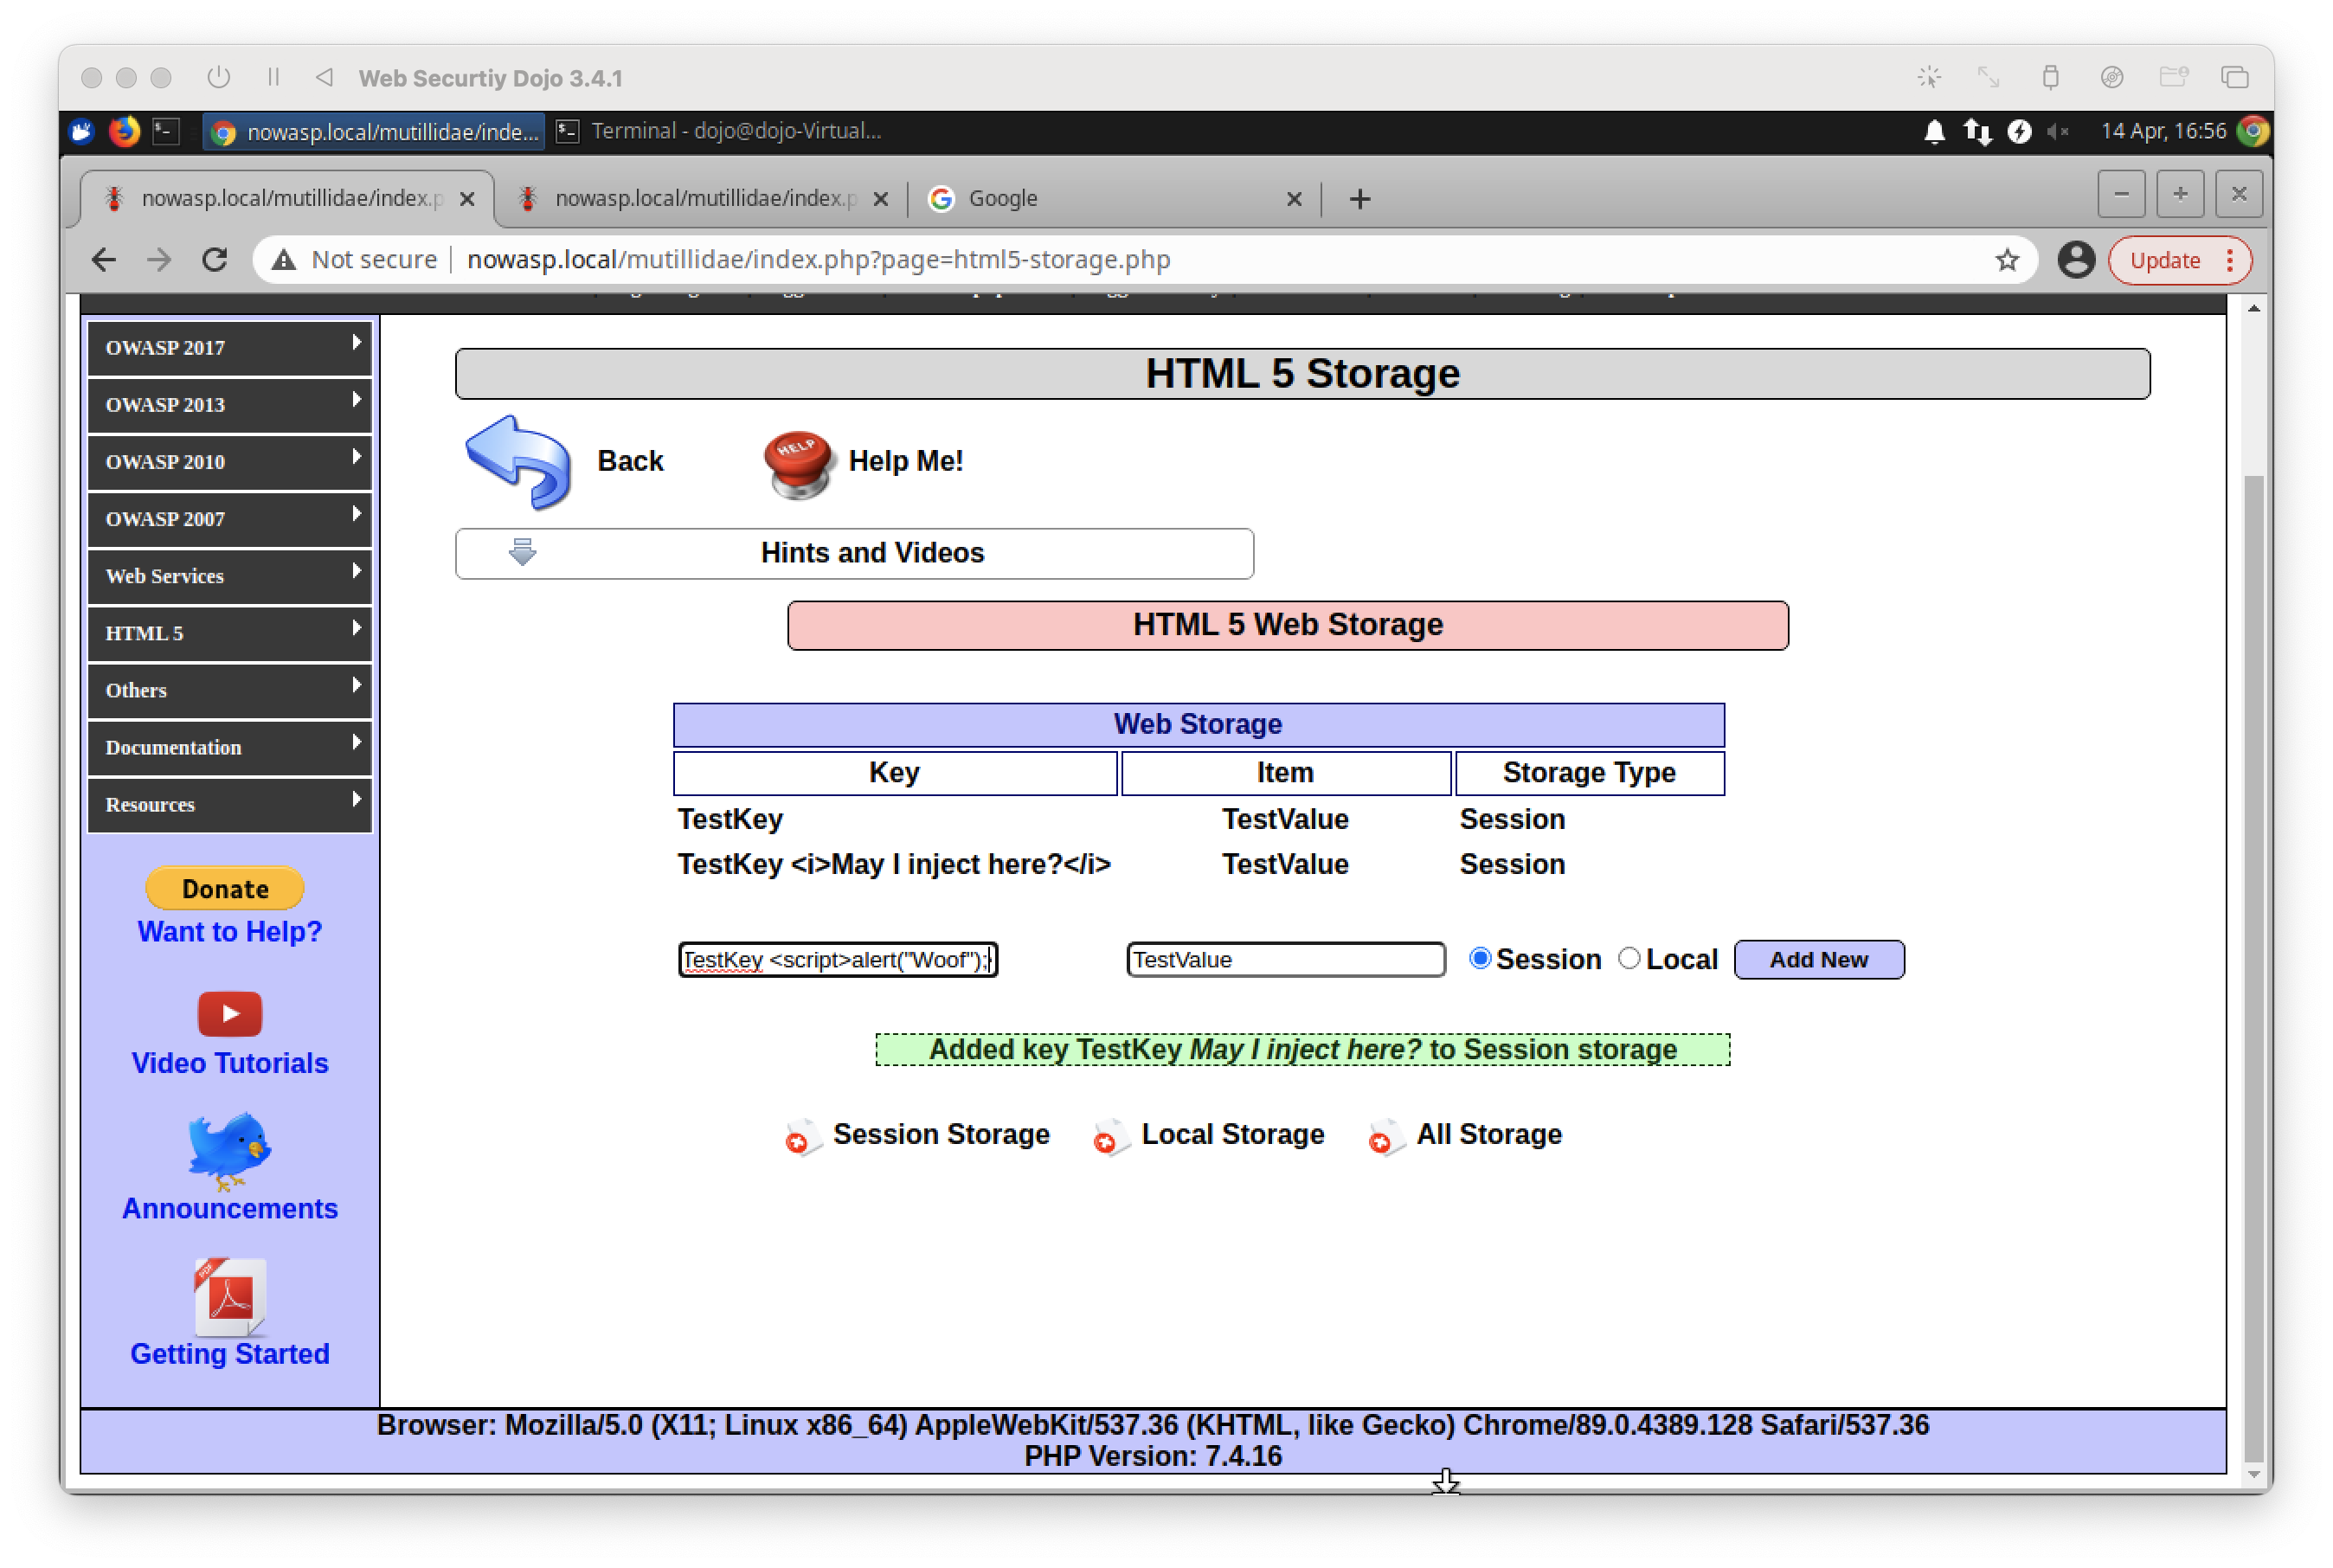
\includegraphics[width=0.8\textwidth]{step_00038}
    \caption{Пробуем встроить JS код}
  \end{figure}

  Т.к. страница после нажатия на кнопку добавления не перезугружалась,
  JS код не выполнился, однако разметка на самом деле применилась.

  \begin{figure}[H]
    \centering
    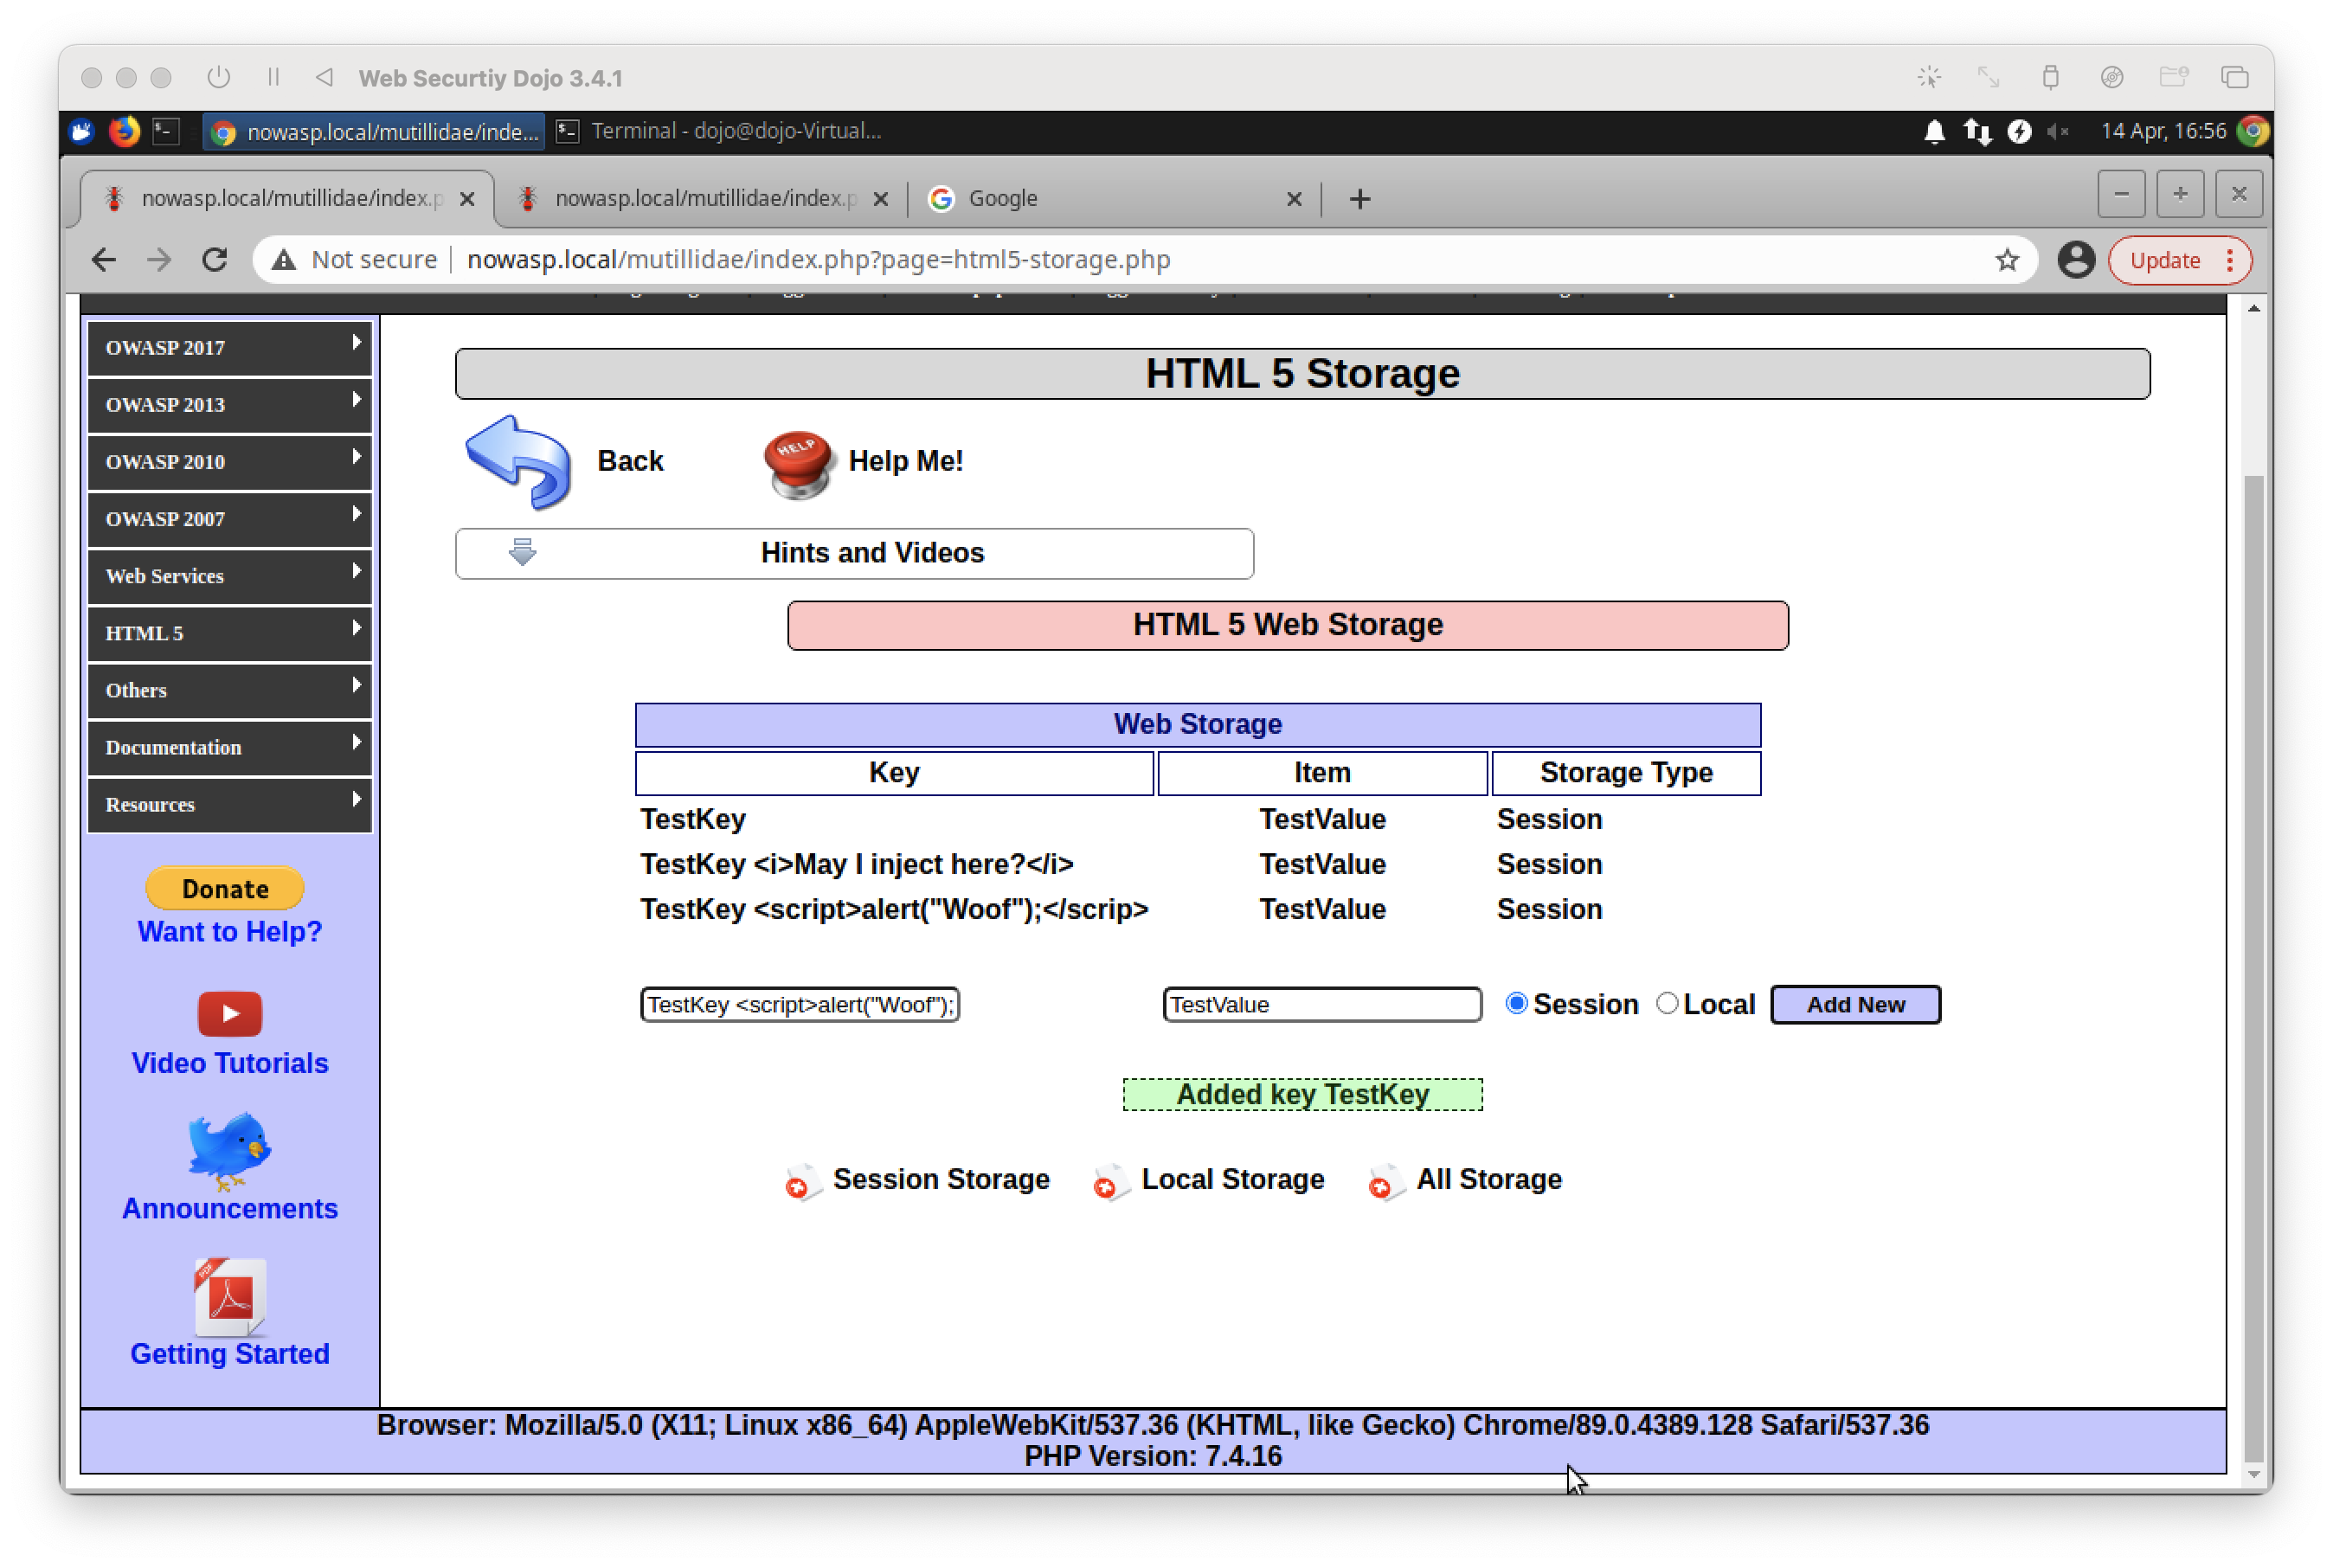
\includegraphics[width=0.8\textwidth]{step_00039}
    \caption{Как будто бы ничего}
  \end{figure}

  \begin{figure}[H]
    \centering
    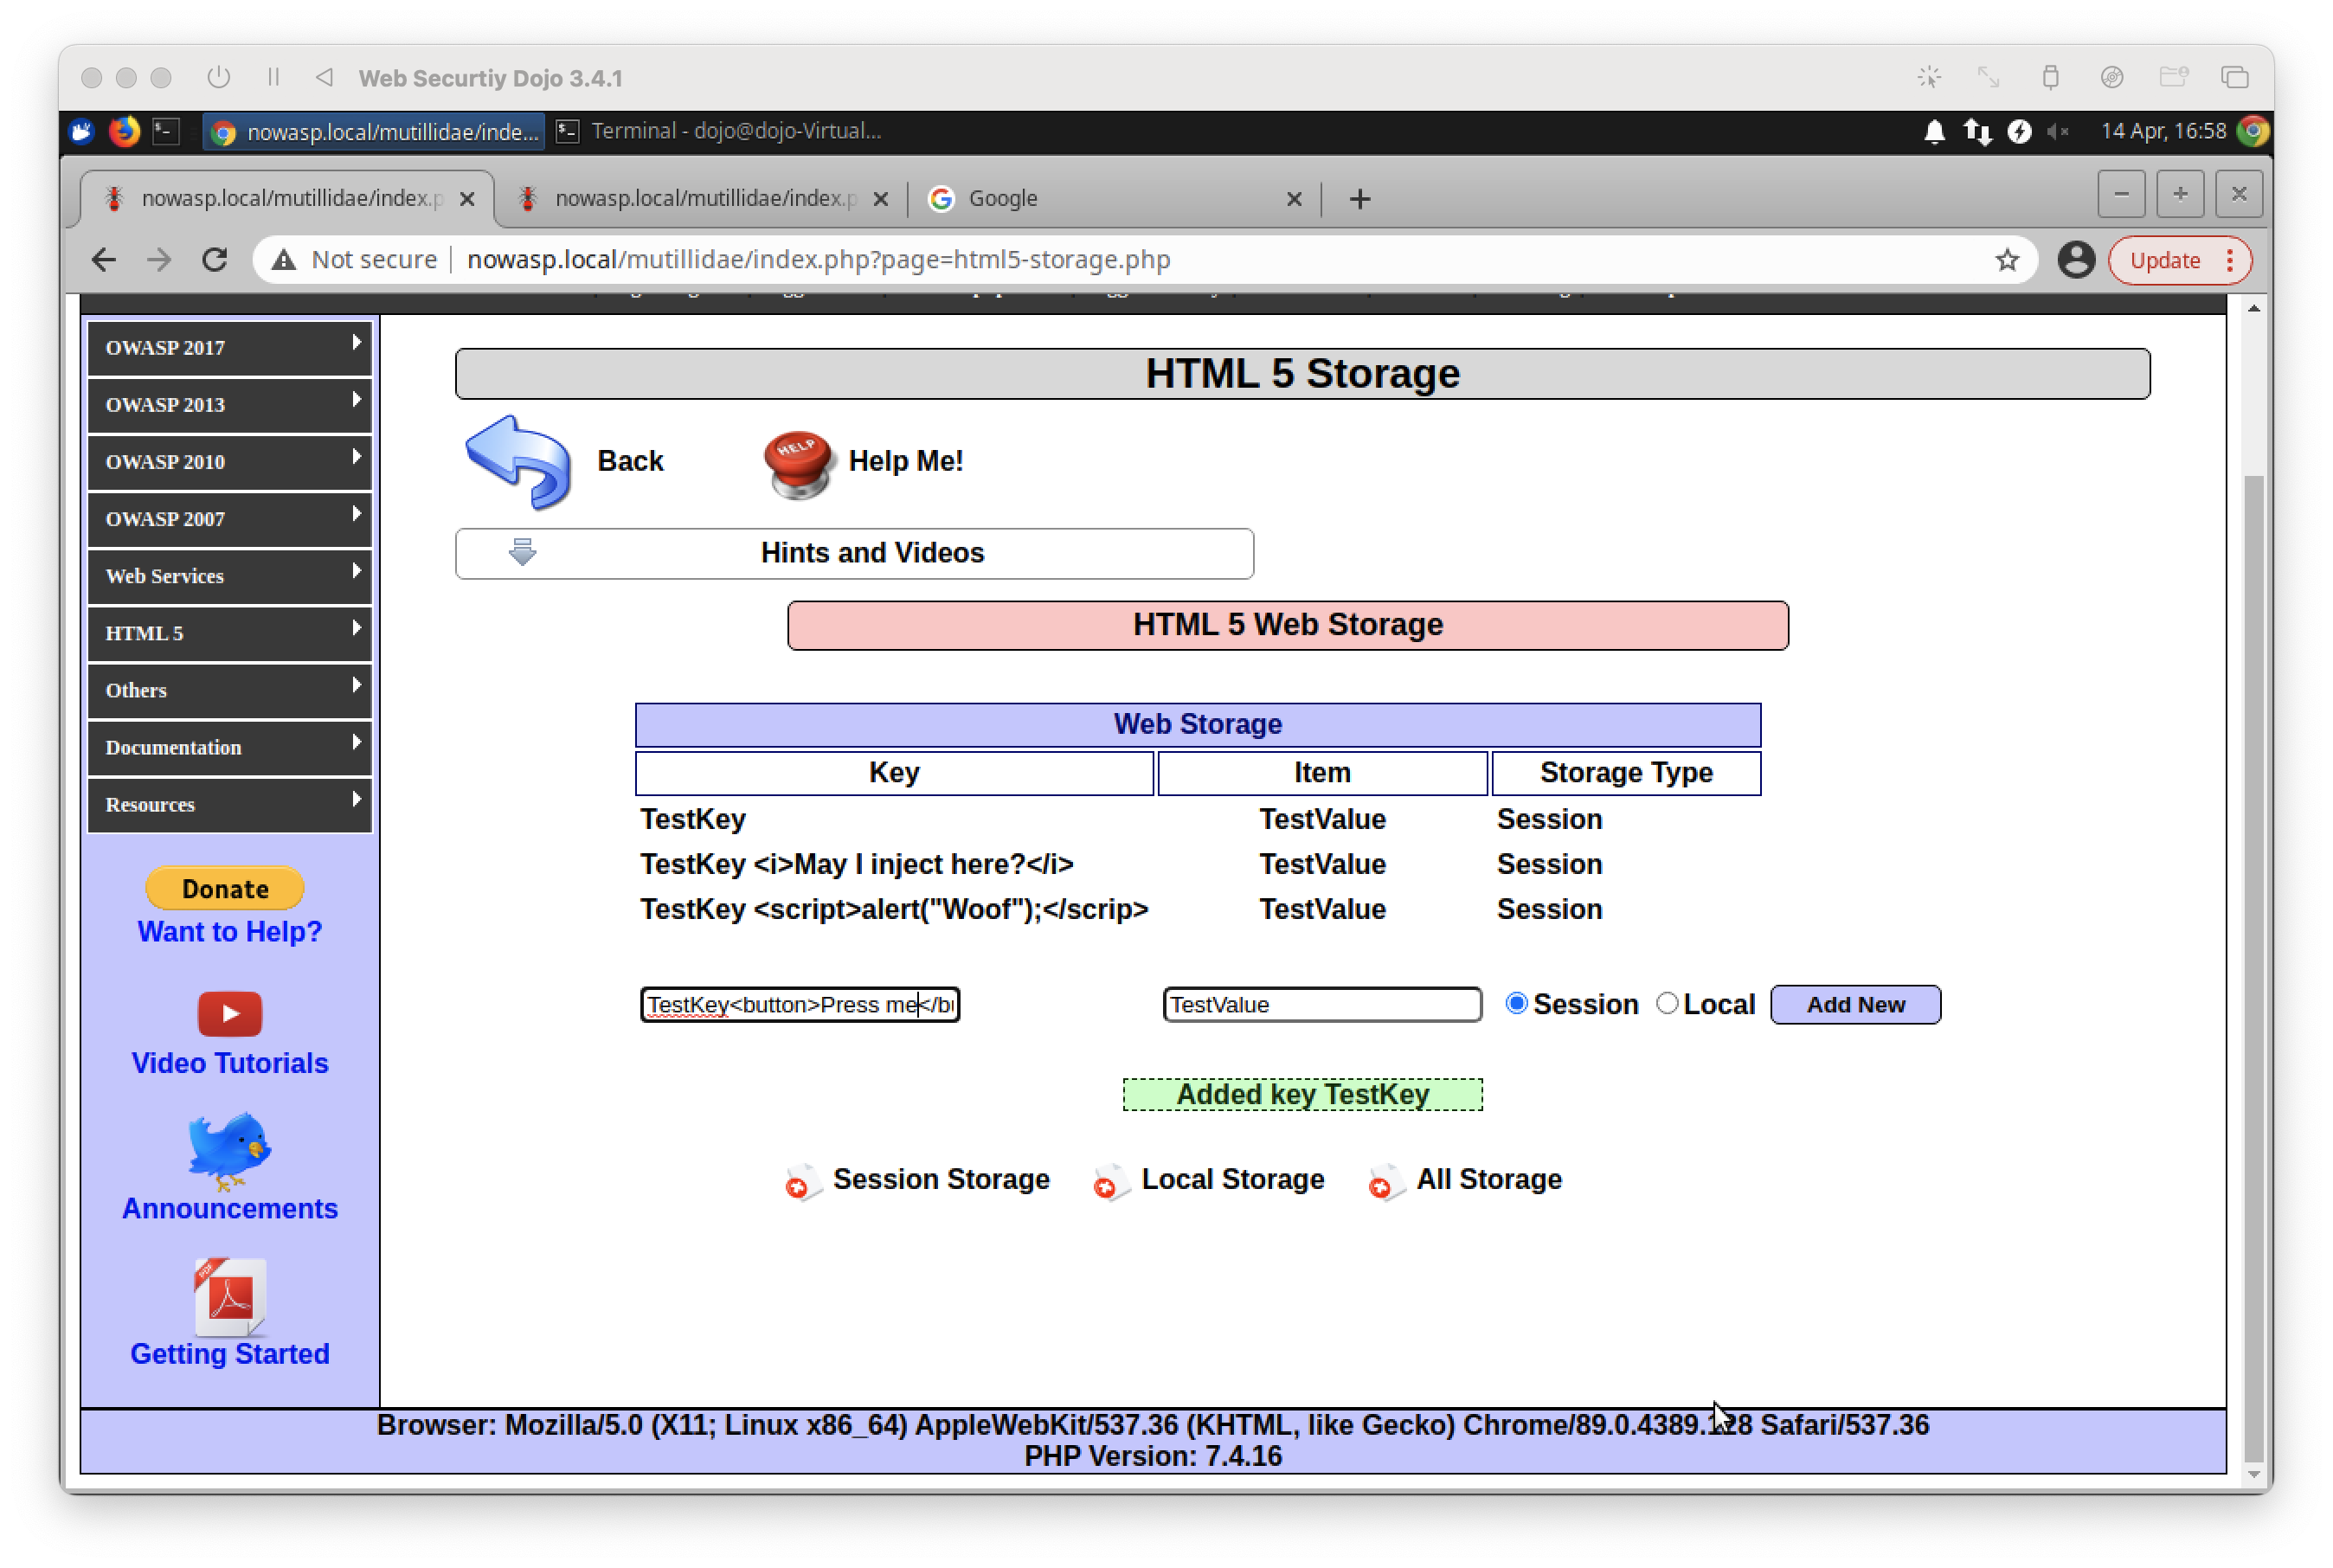
\includegraphics[width=0.8\textwidth]{step_00040}
    \caption{Не можем встроить код - встроим кнопку}
  \end{figure}

  \begin{figure}[H]
    \centering
    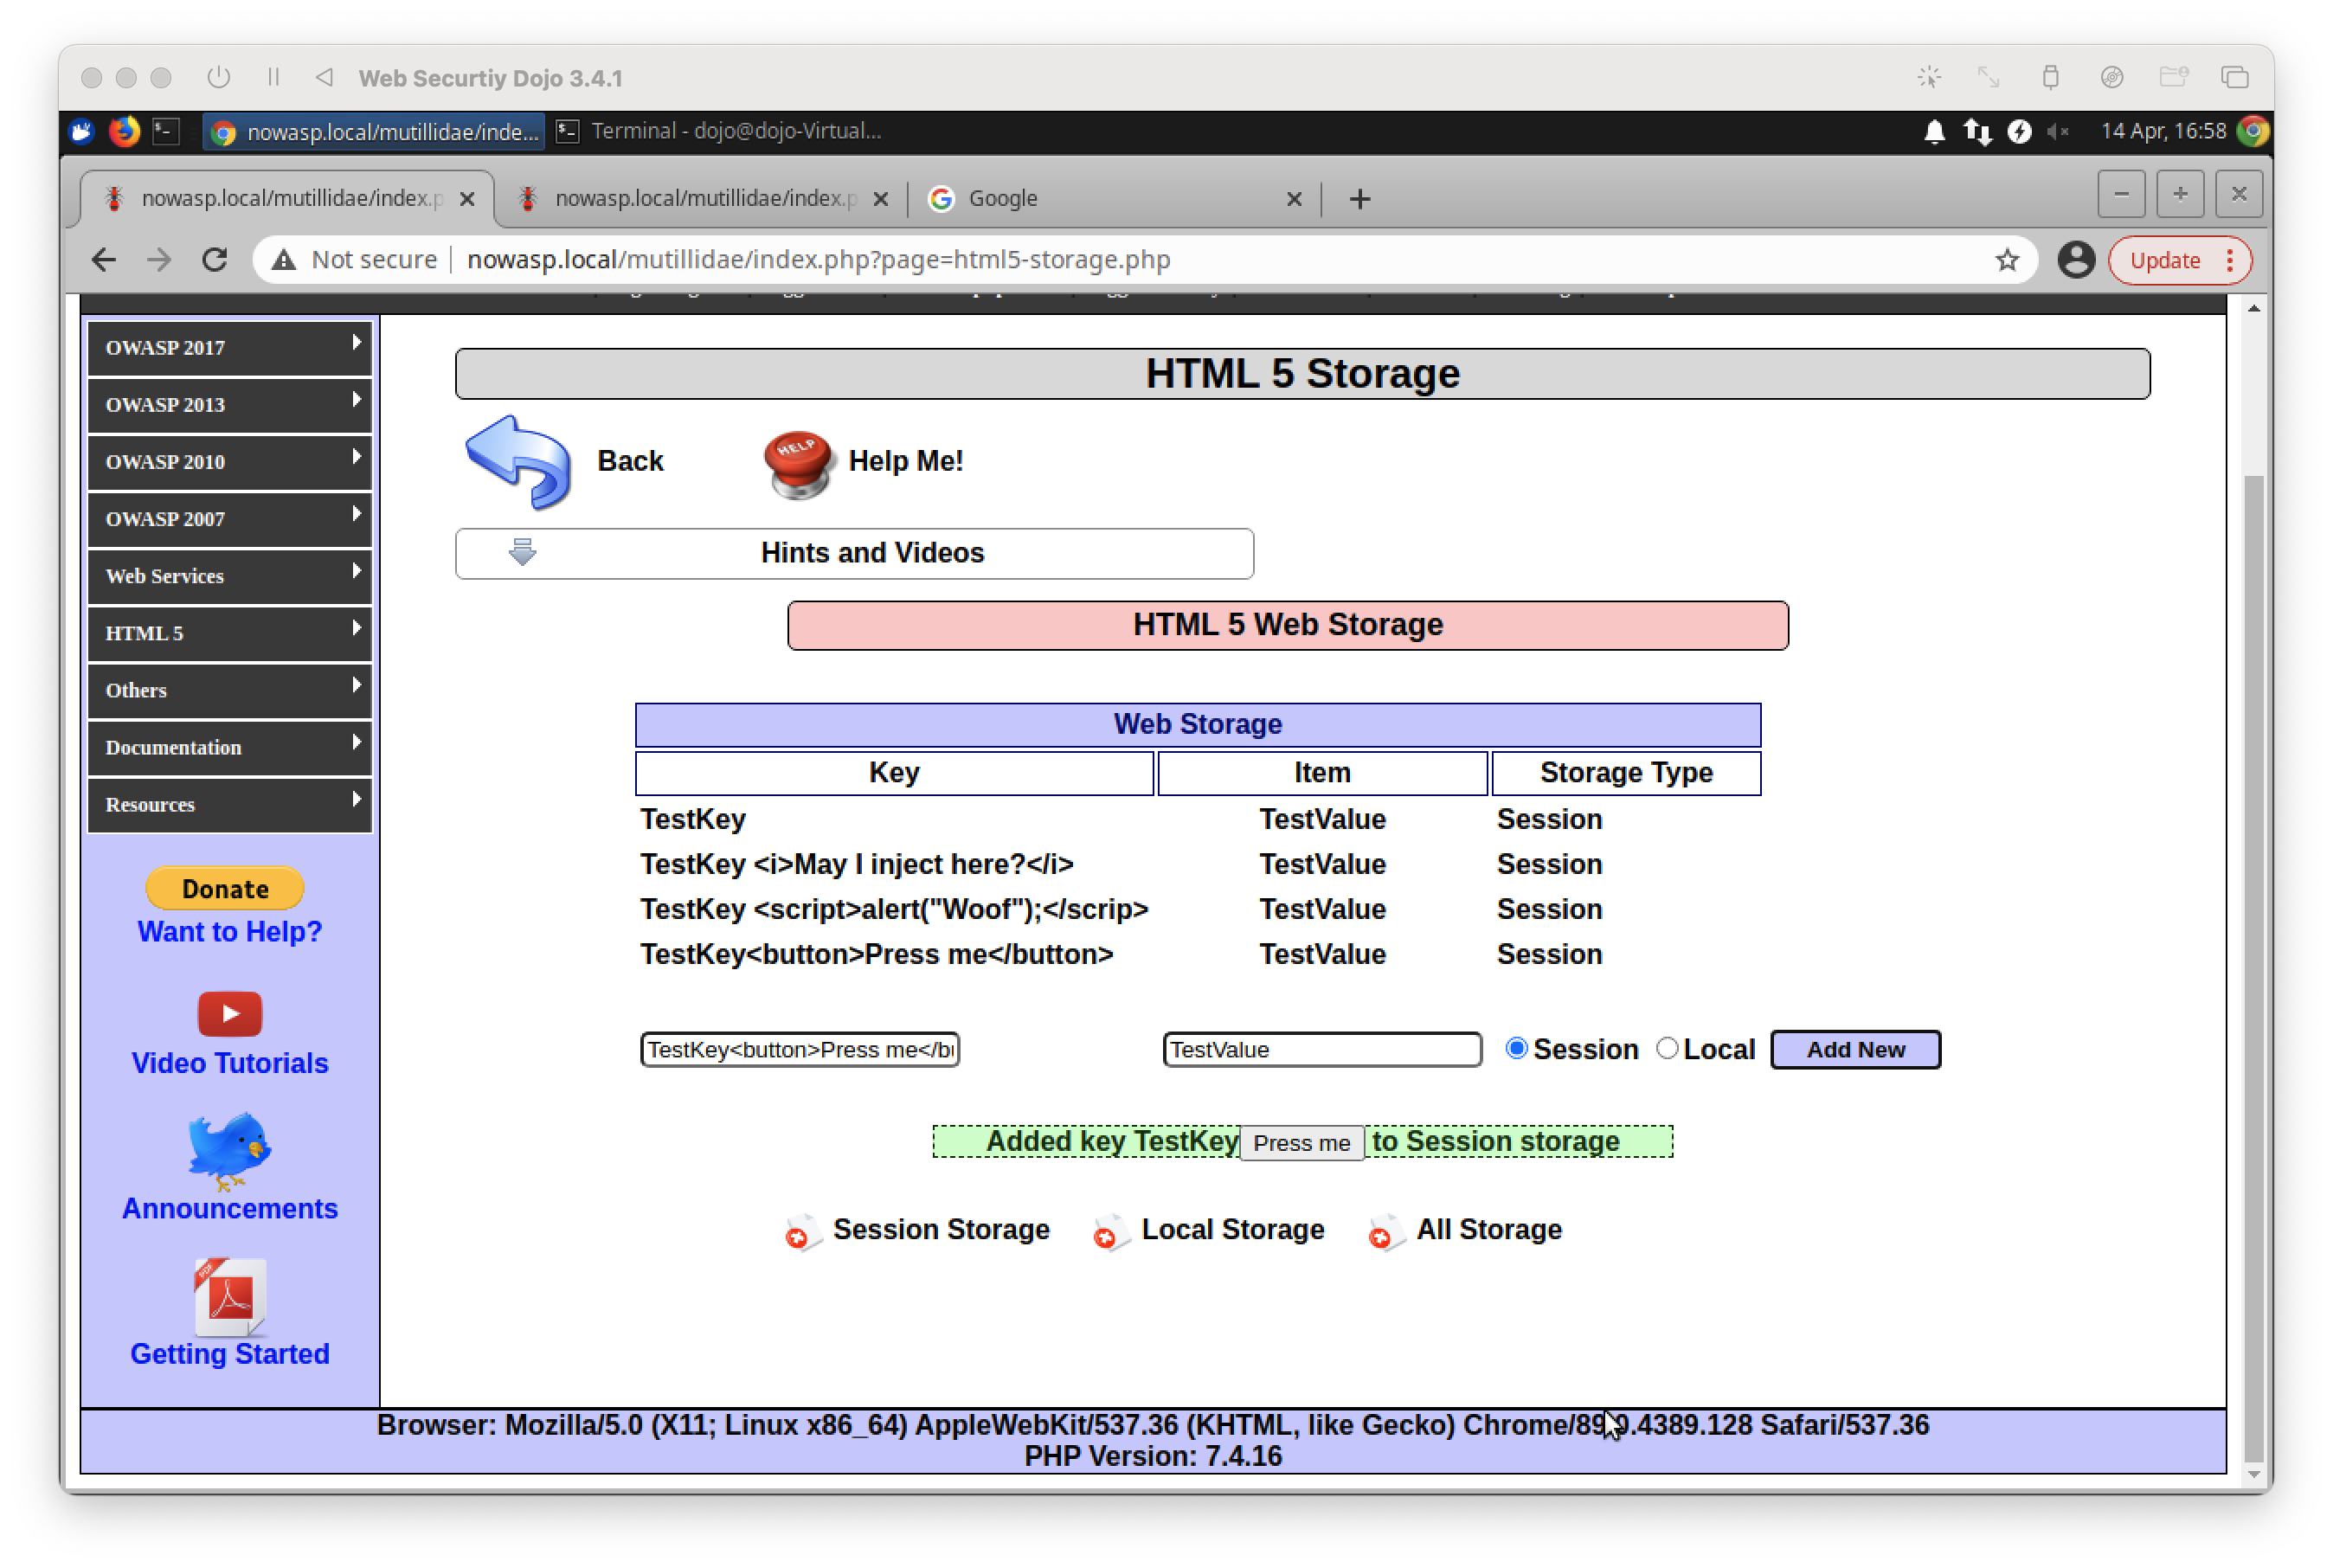
\includegraphics[width=0.8\textwidth]{step_00041}
    \caption{Кнопка}
  \end{figure}

  \begin{figure}[H]
    \centering
    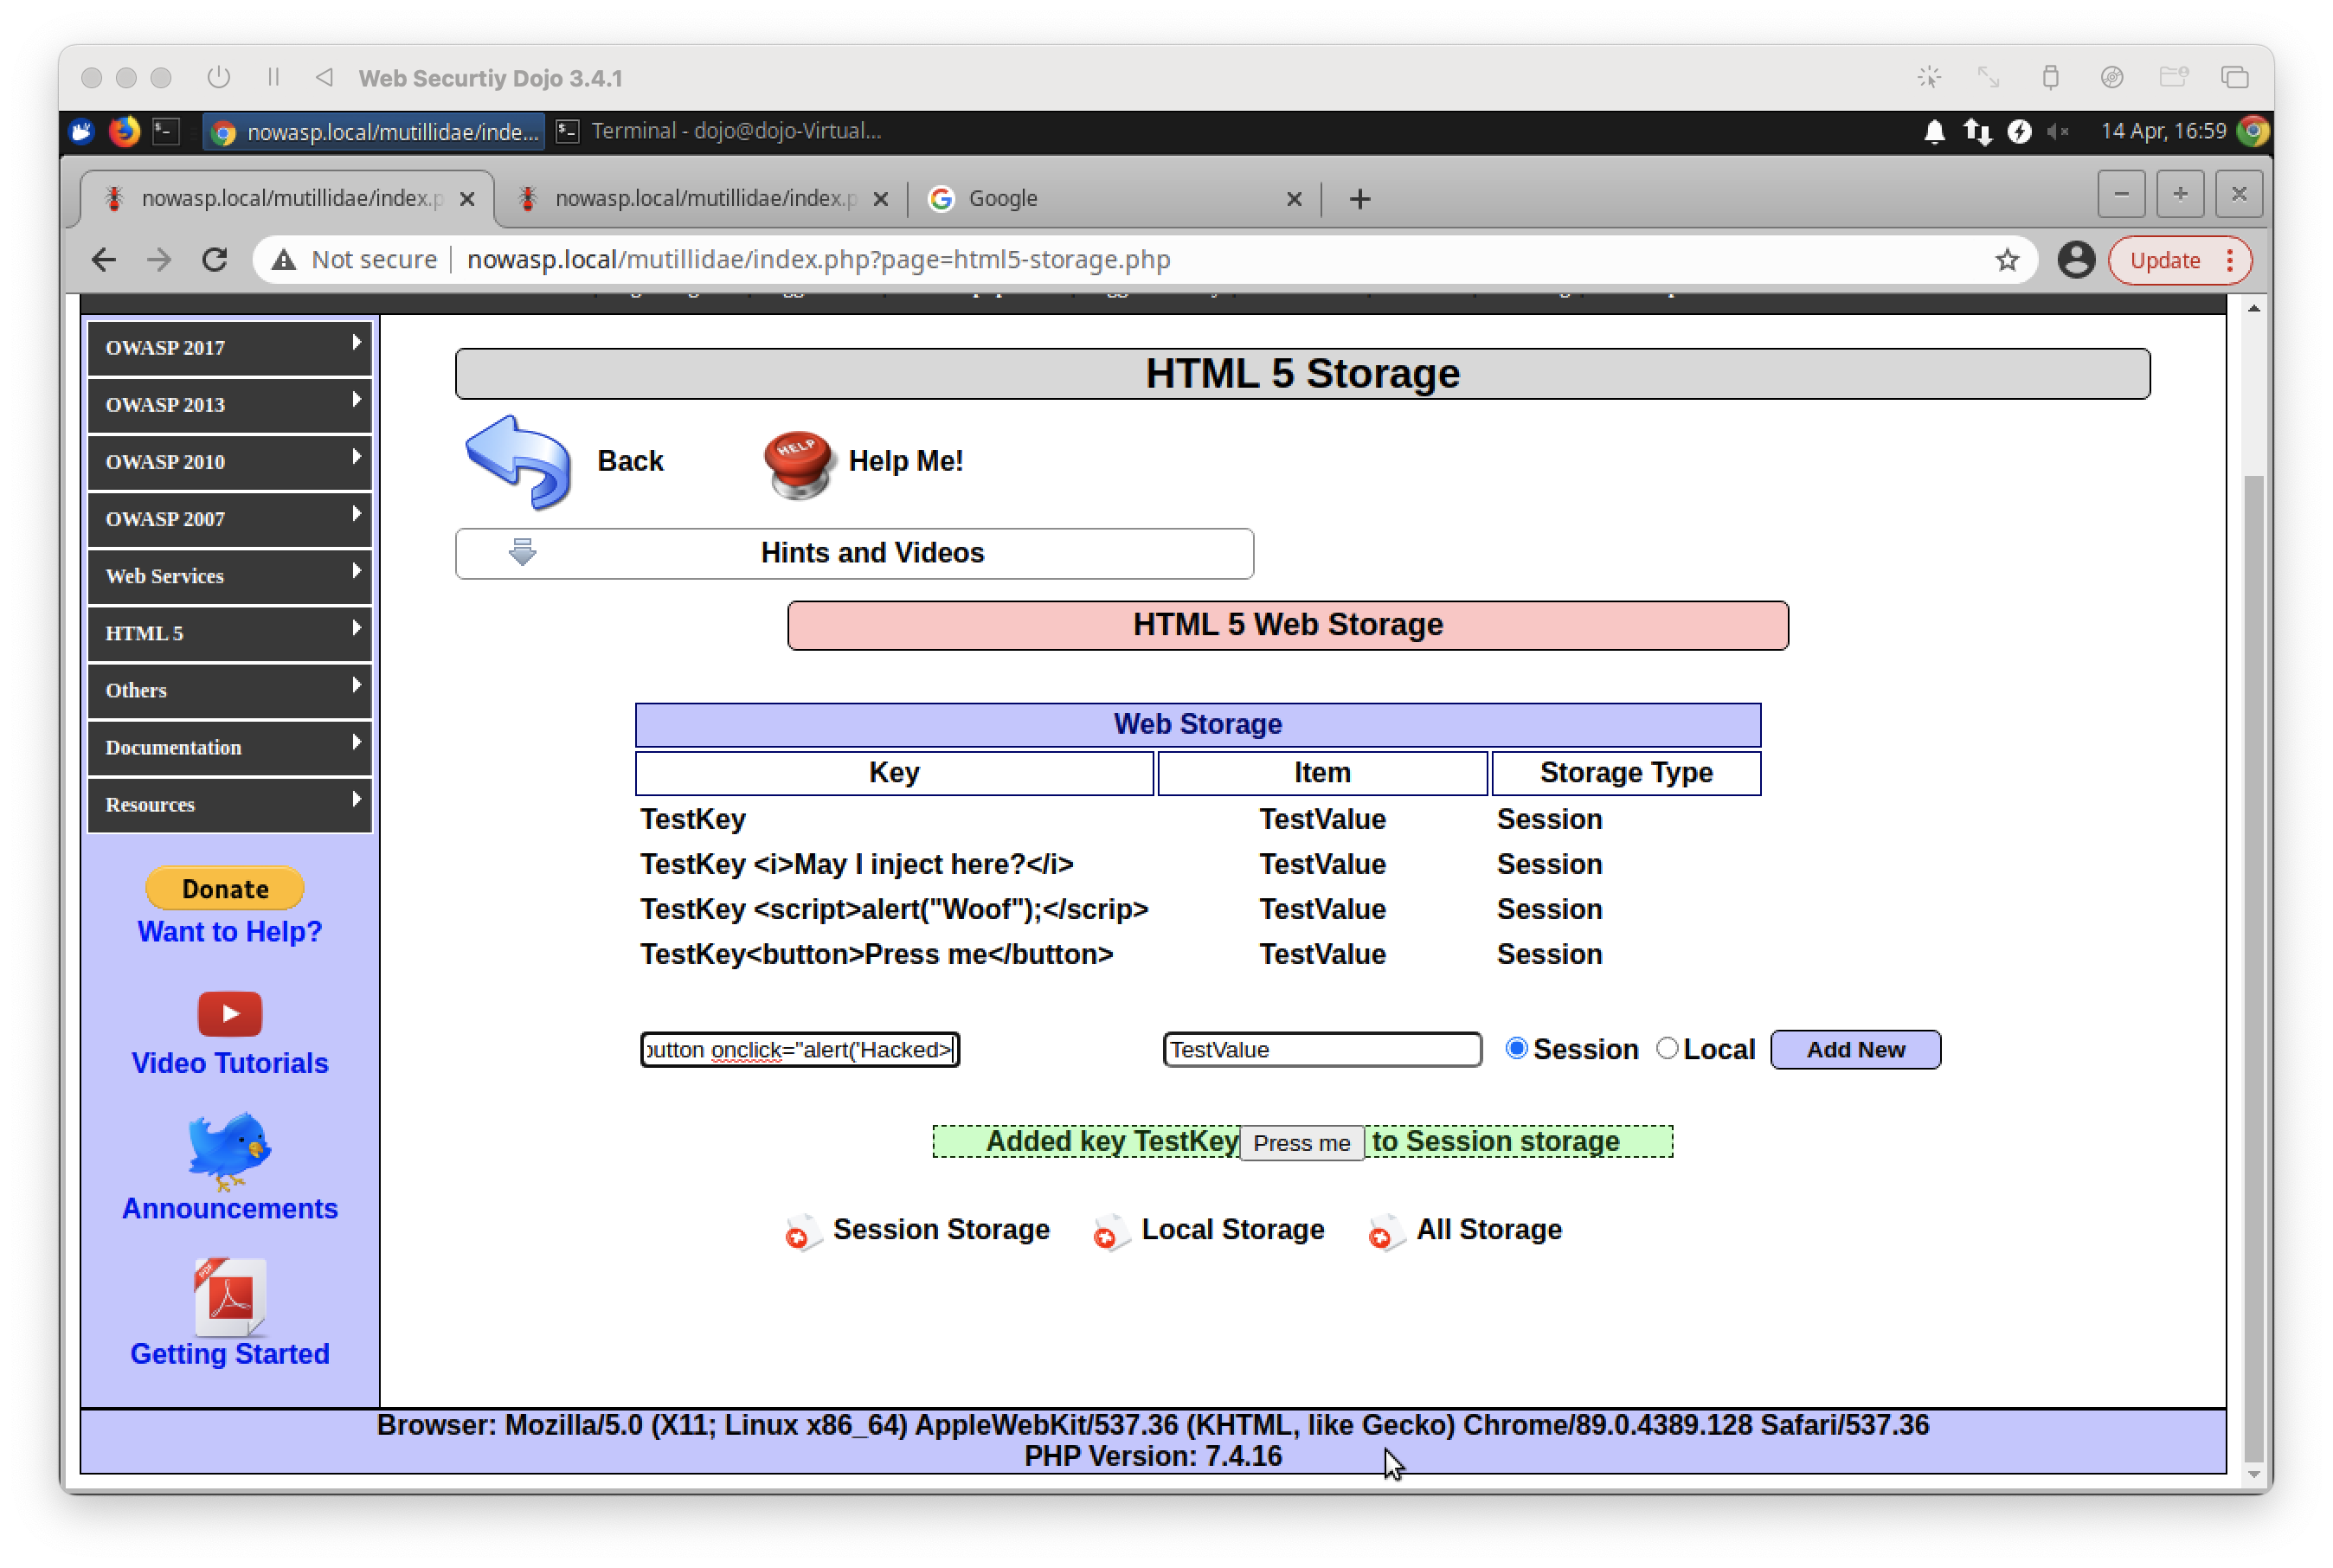
\includegraphics[width=0.8\textwidth]{step_00042}
    \caption{Добавим кнопке атрибут onclick, чтобы по нажатию на неё выводилось сообщение}
  \end{figure}

  \begin{figure}[H]
    \centering
    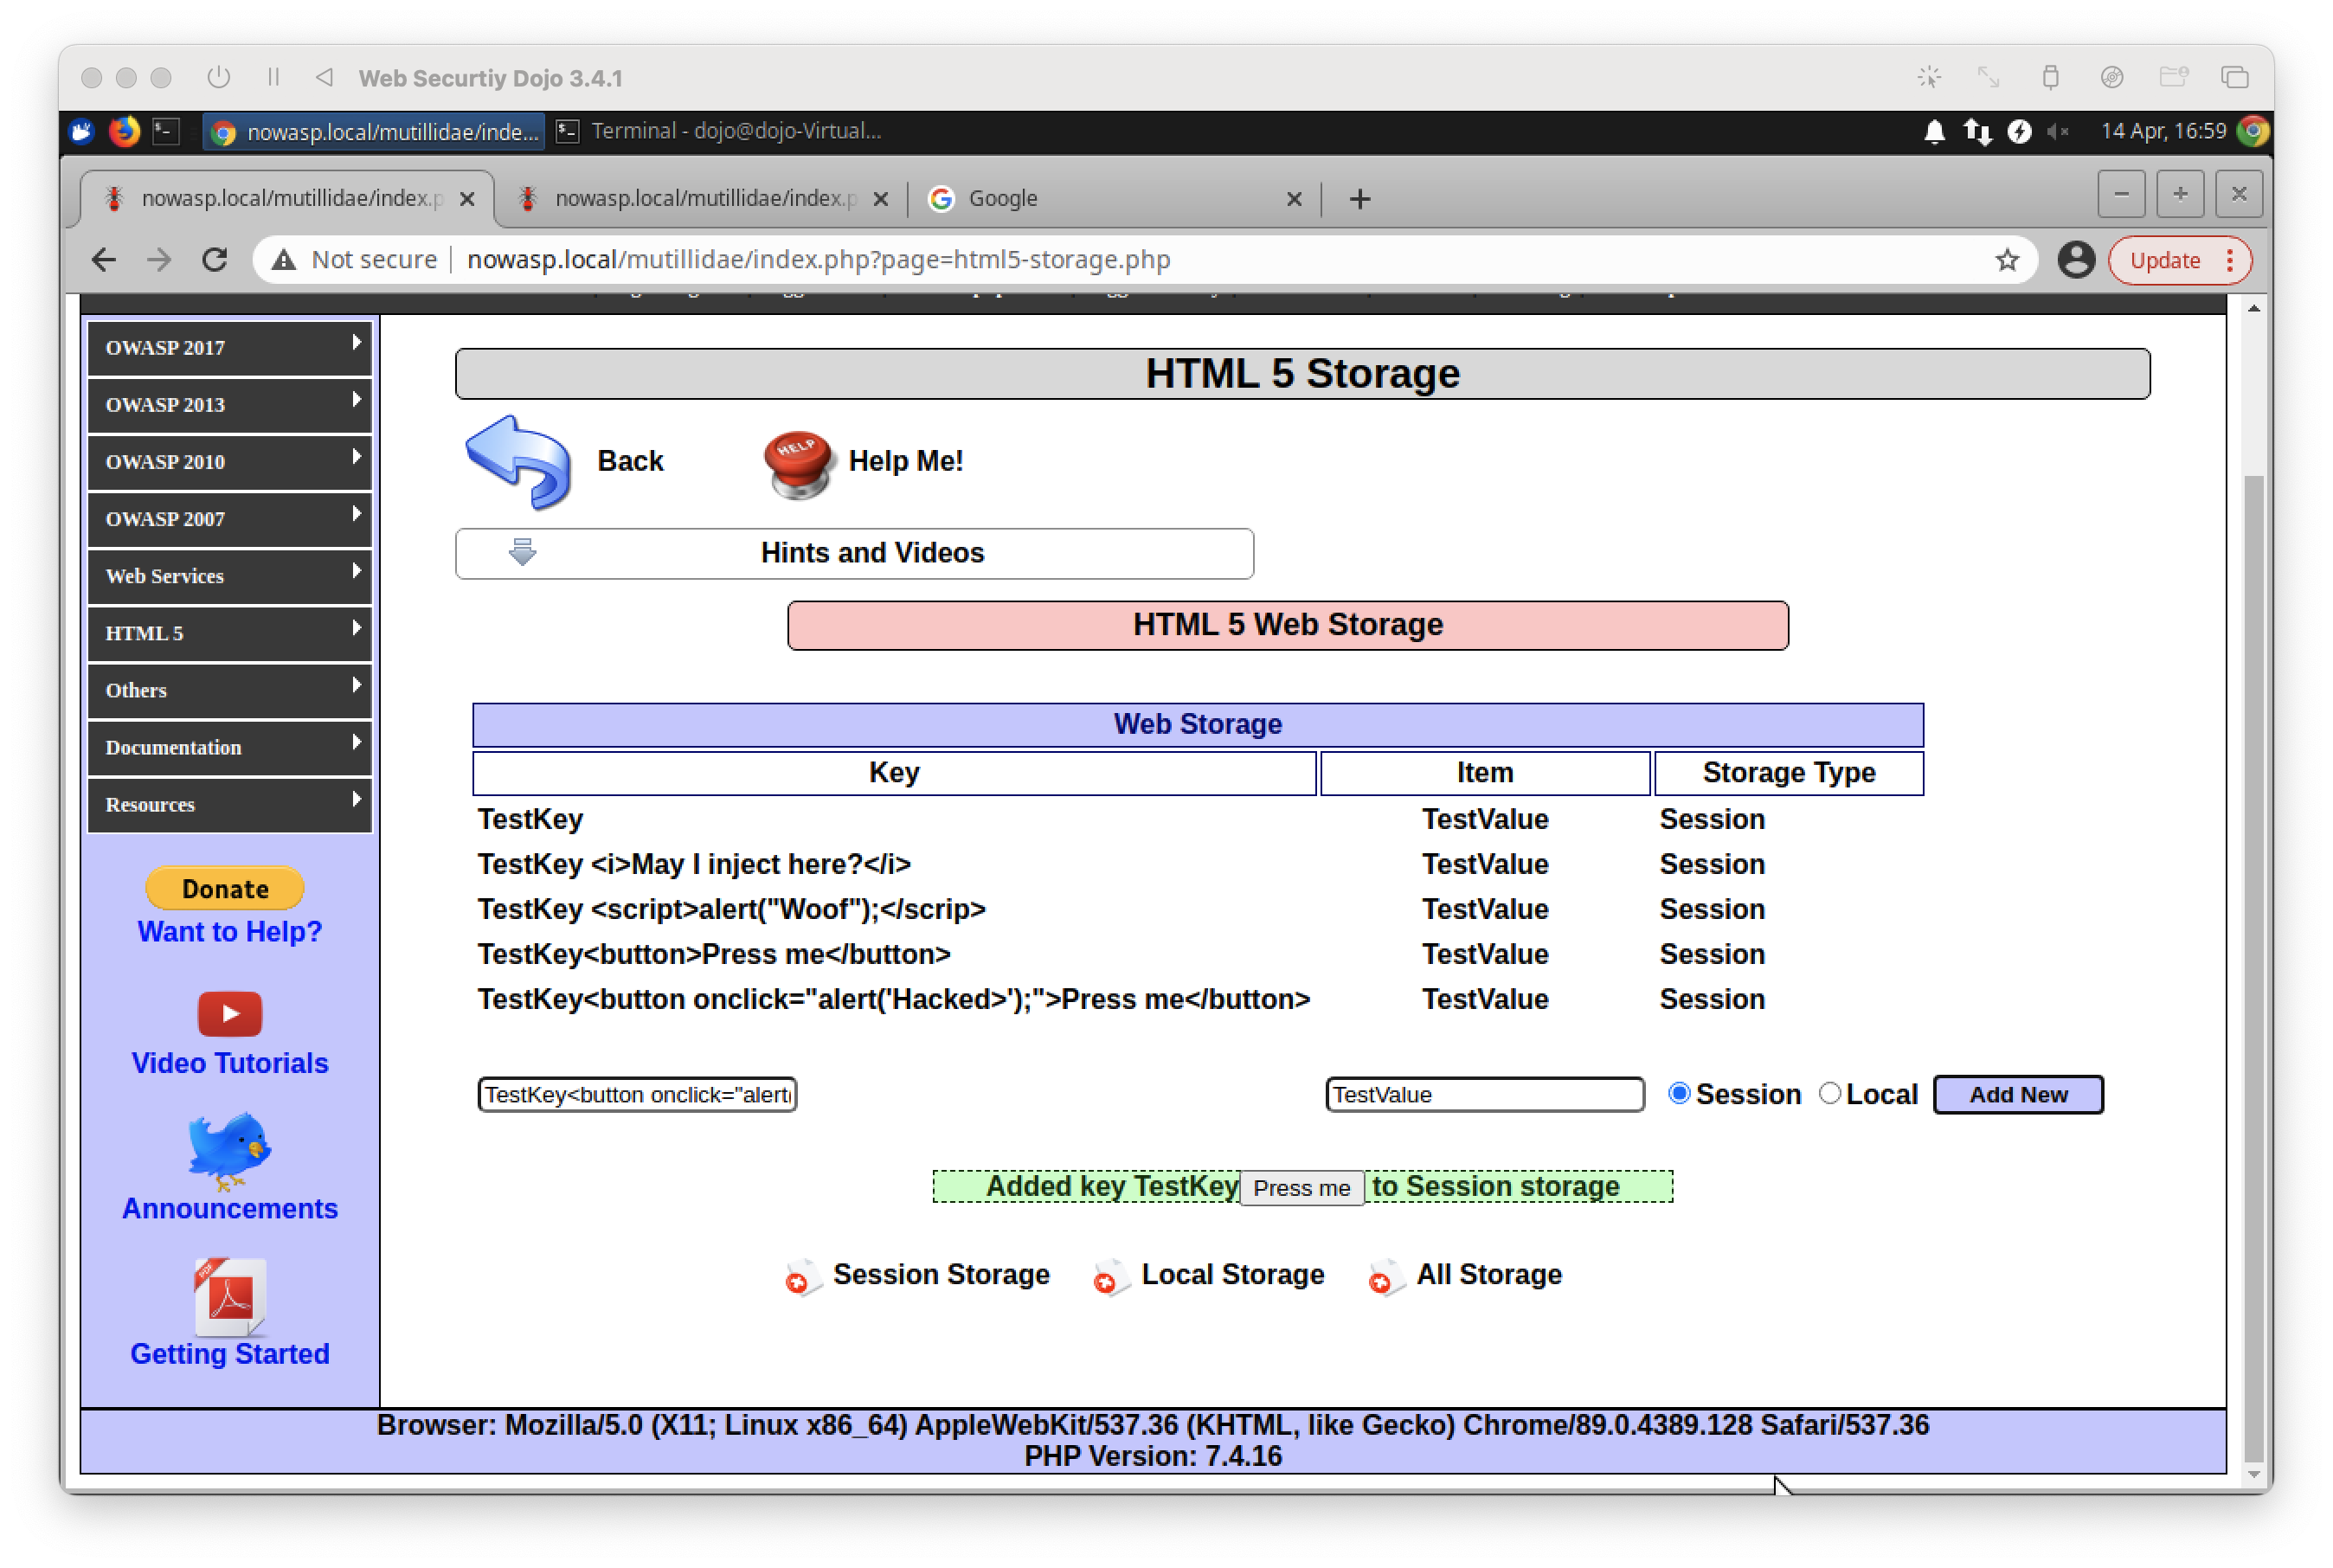
\includegraphics[width=0.8\textwidth]{step_00043}
    \caption{Кнопка с обработчиком нажатия установлена}
  \end{figure}

  \begin{figure}[H]
    \centering
    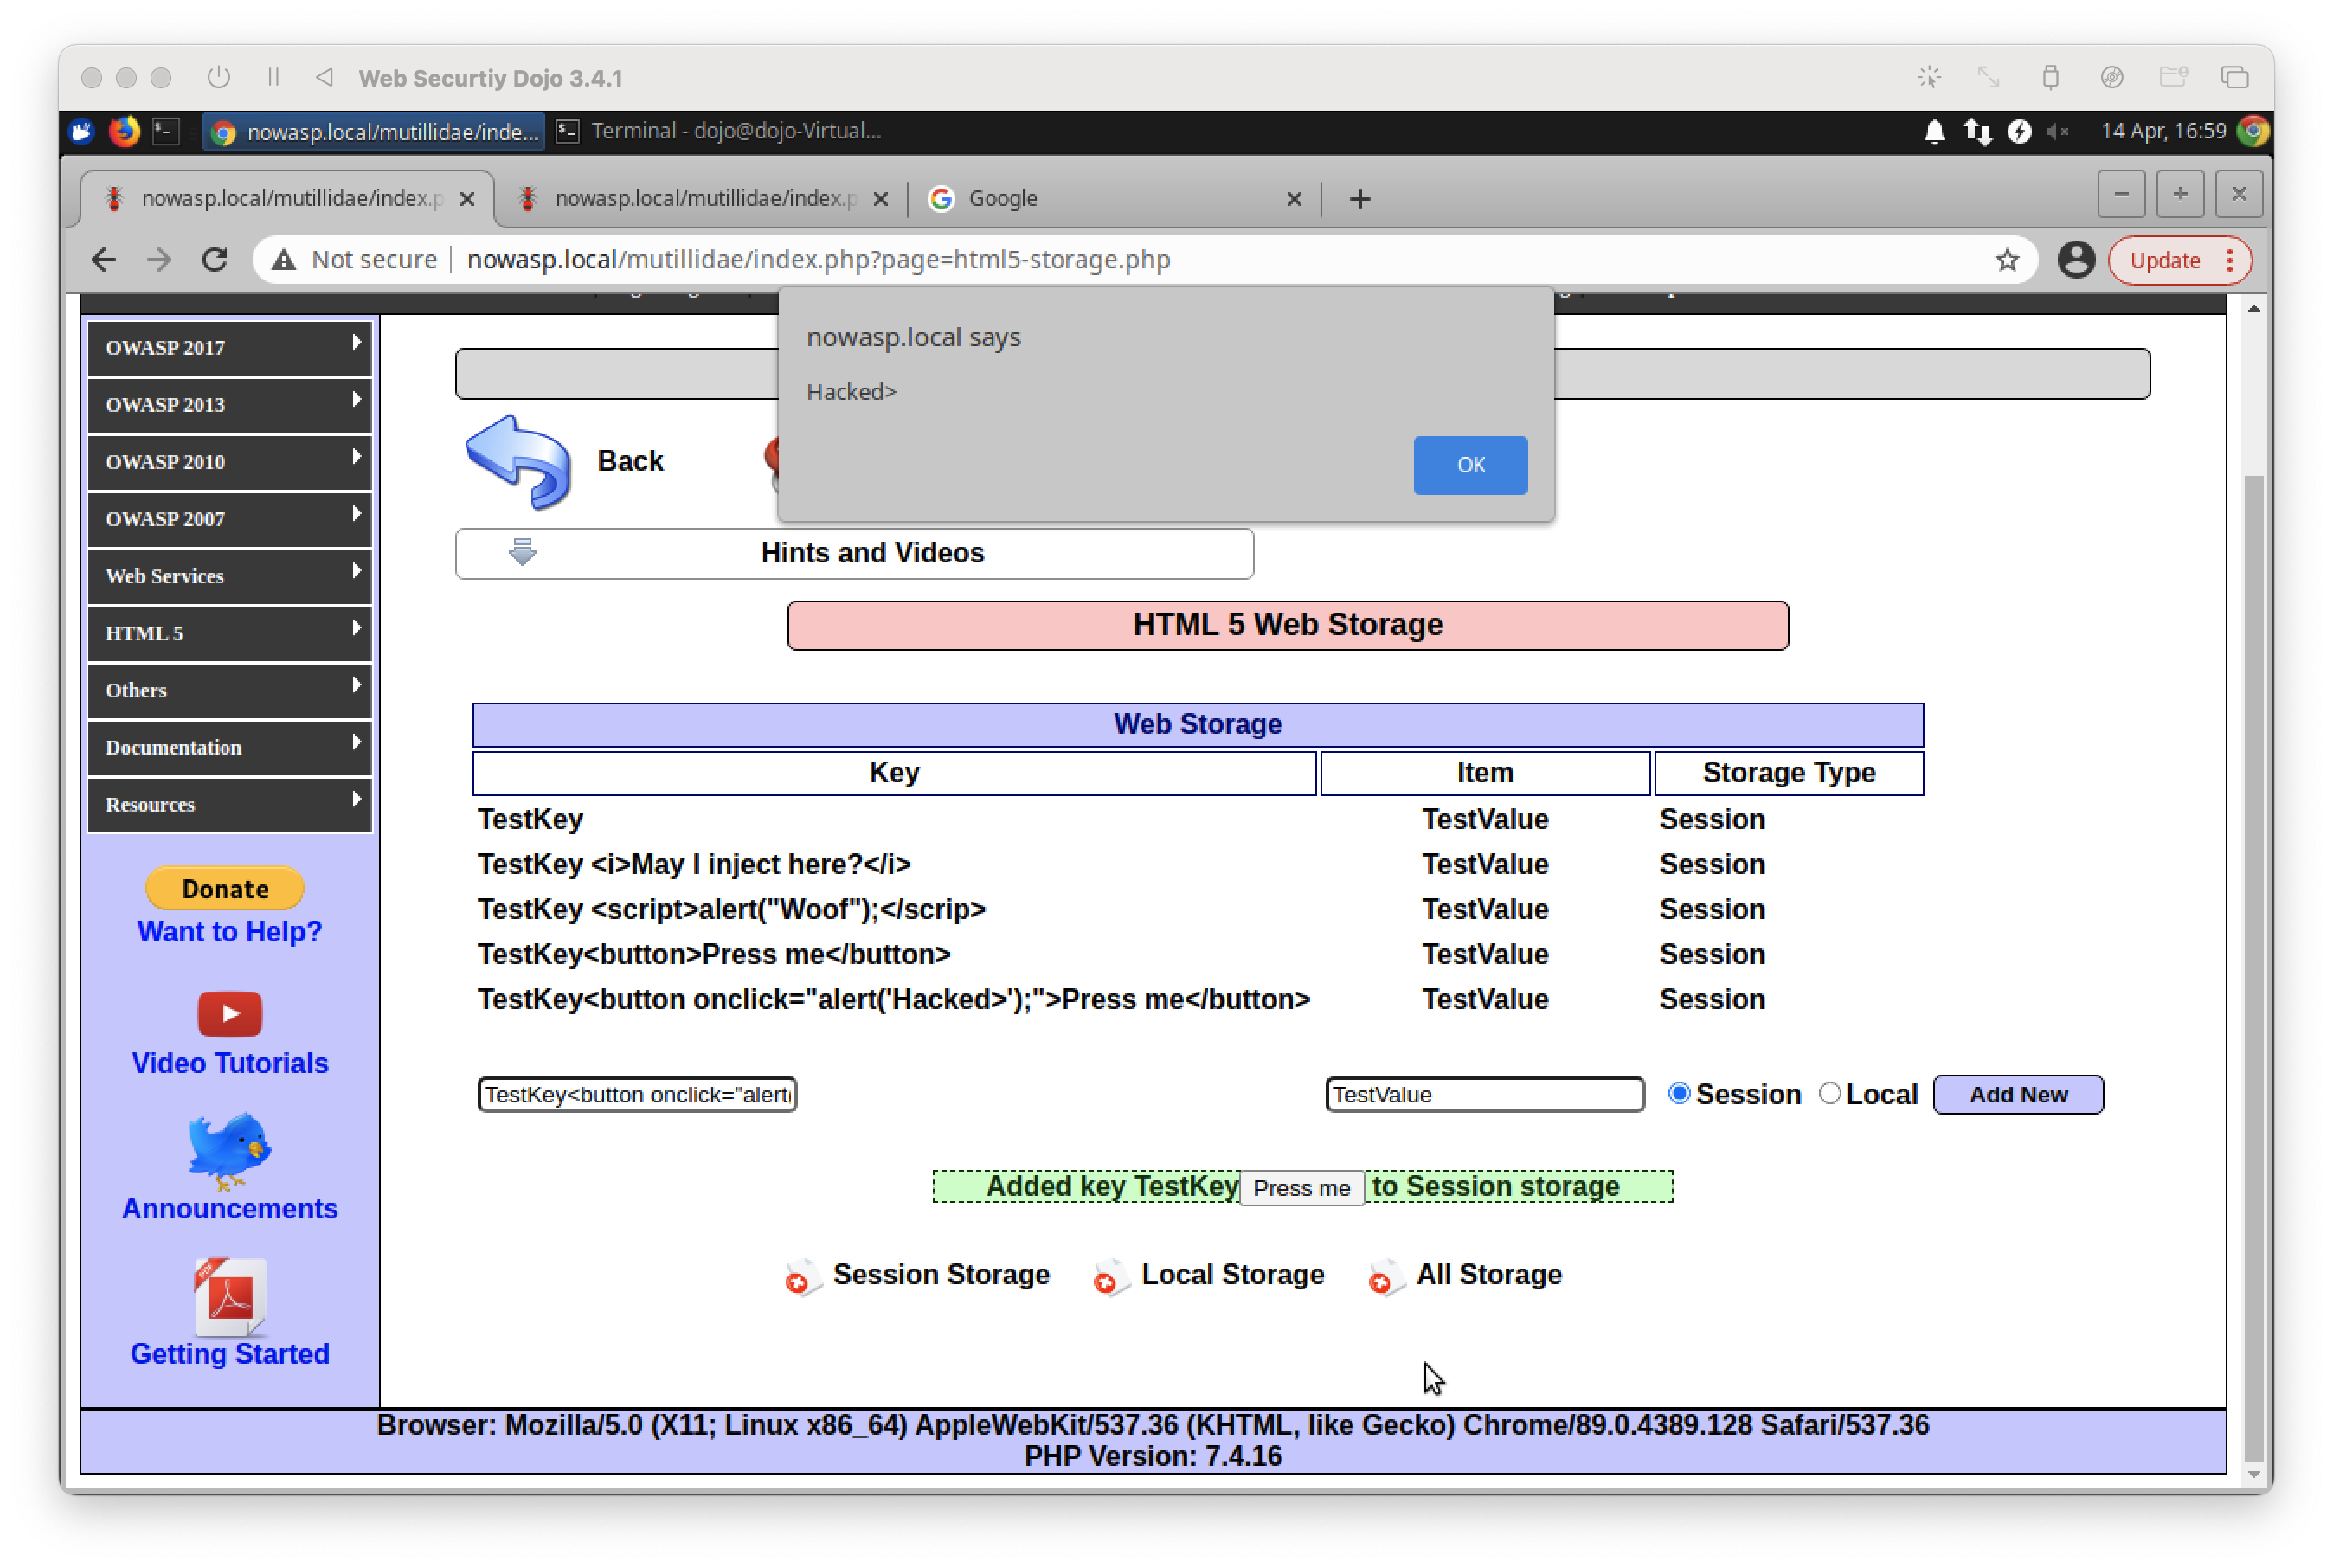
\includegraphics[width=0.8\textwidth]{step_00044}
    \caption{Кнопка работает}
  \end{figure}

  \begin{figure}[H]
    \centering
    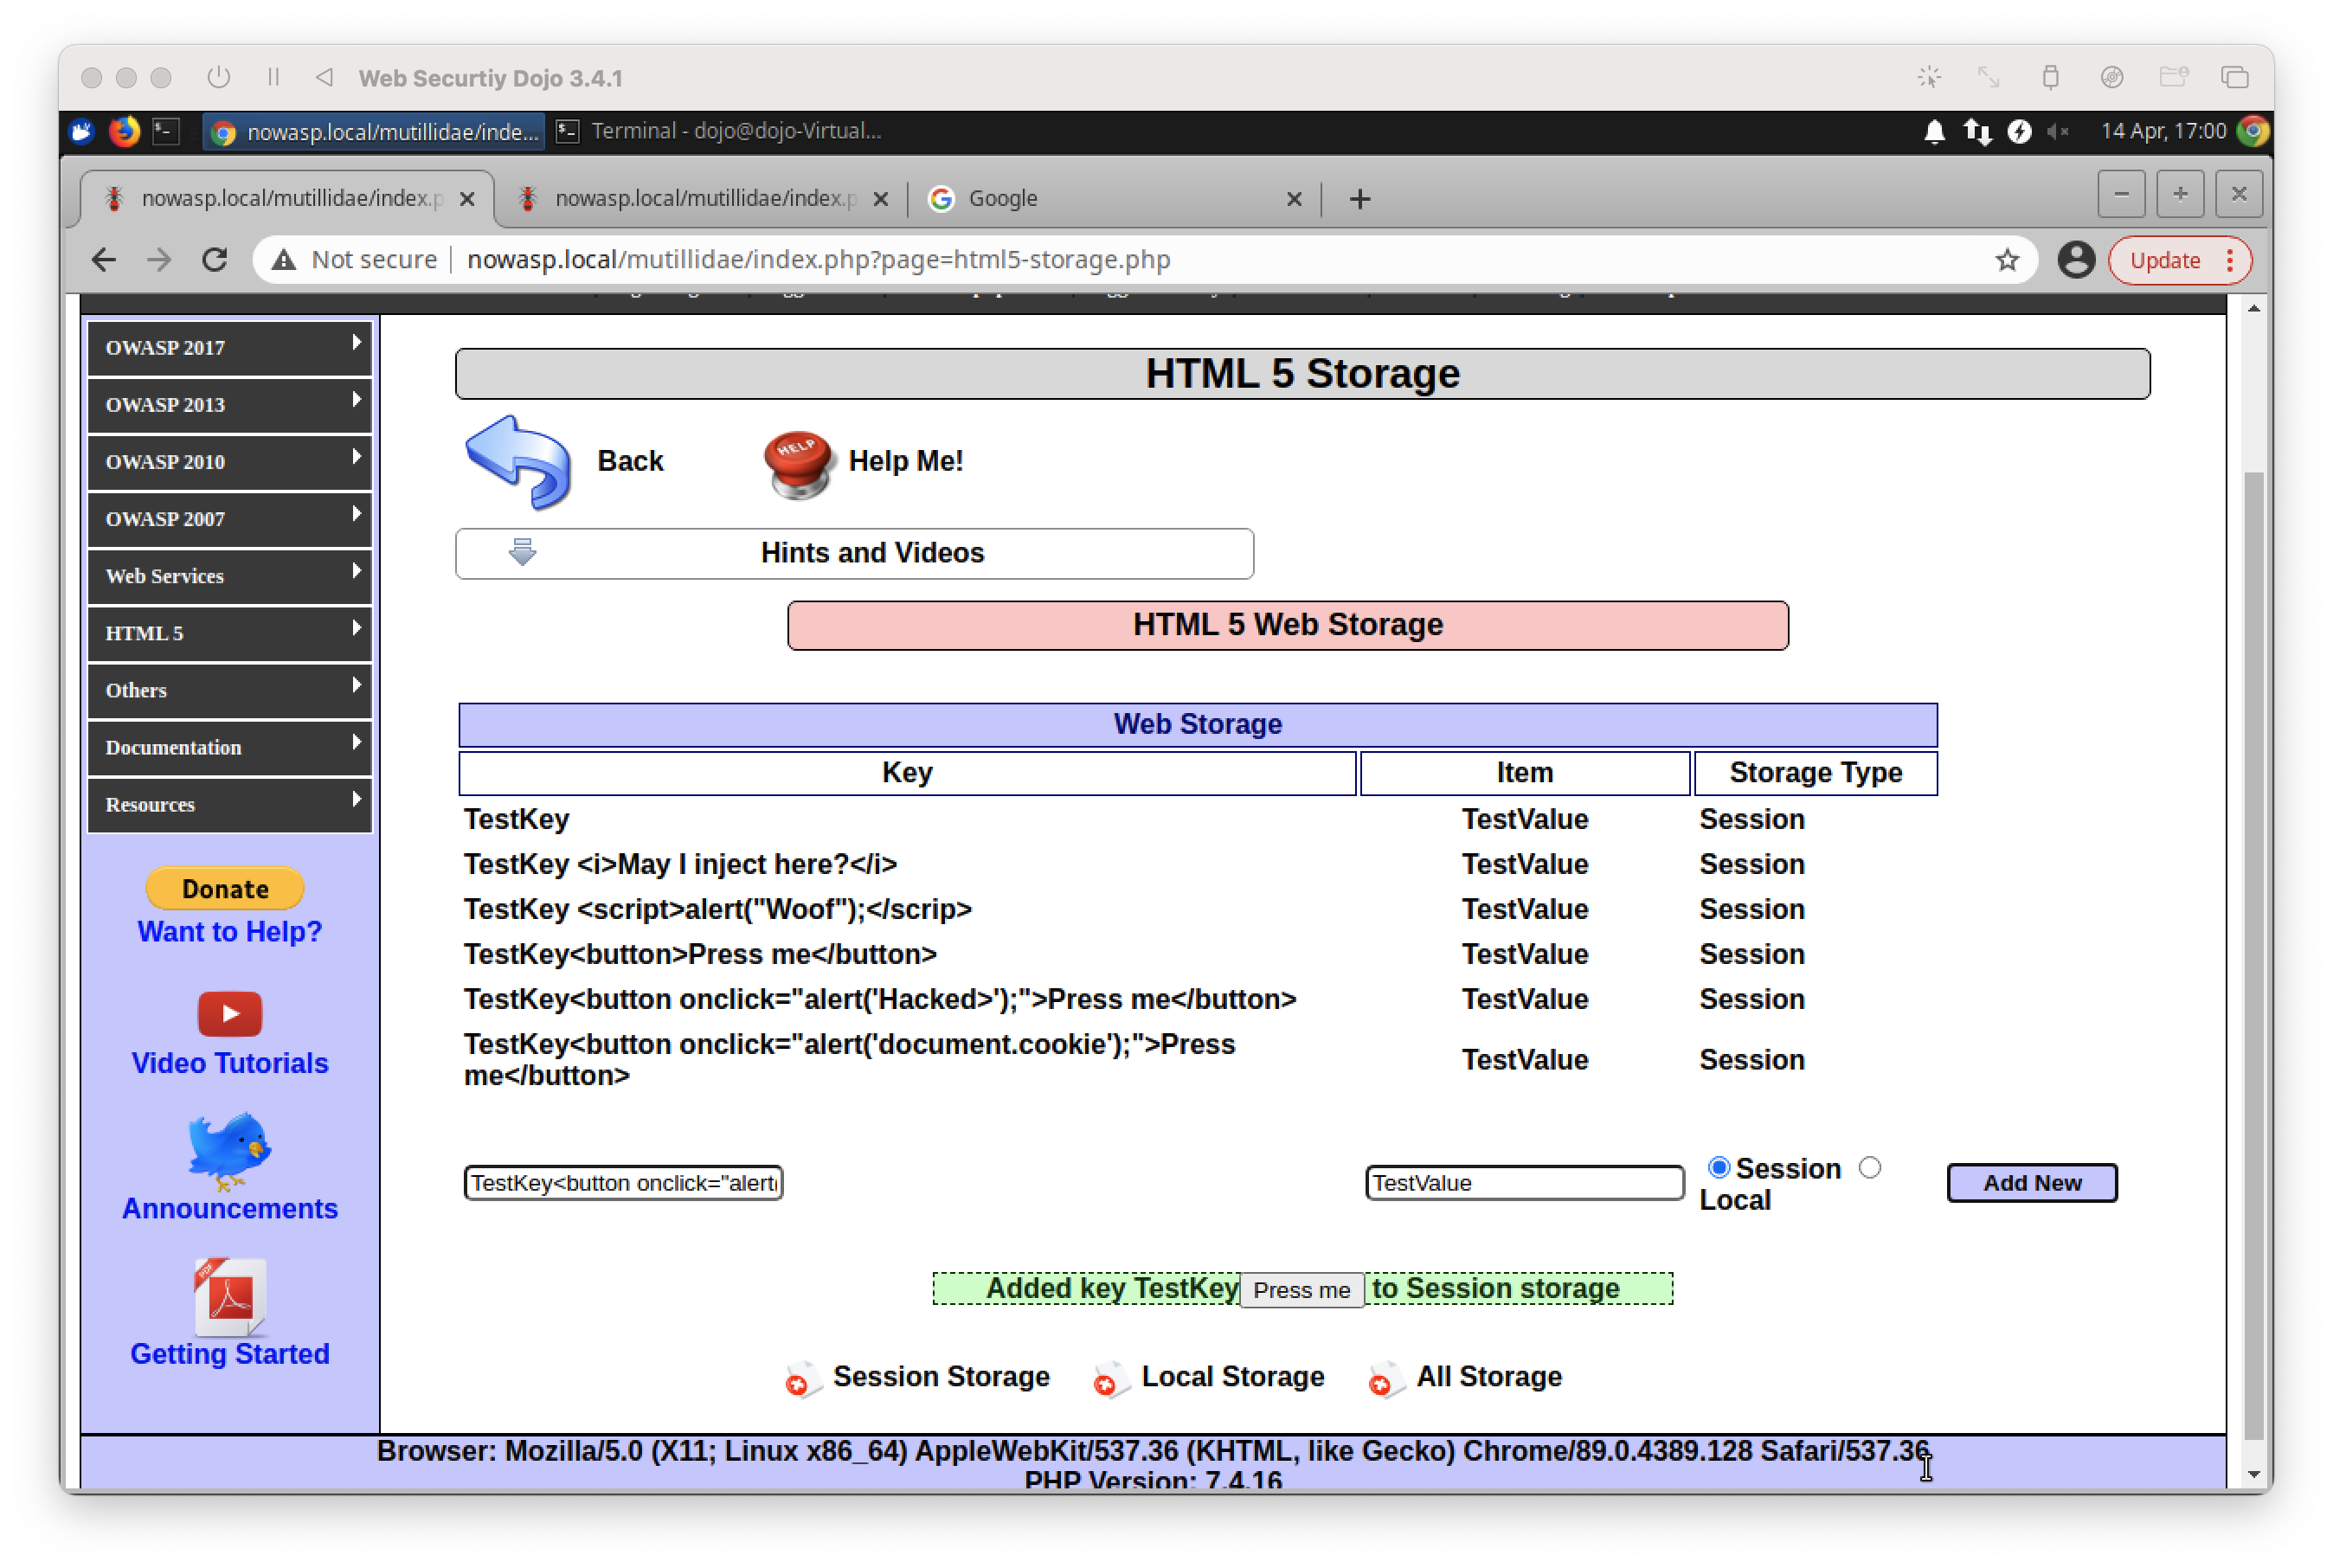
\includegraphics[width=0.8\textwidth]{step_00045}
    \caption{Таким образом можно укарсть cookie}
  \end{figure}

  \begin{figure}[H]
    \centering
    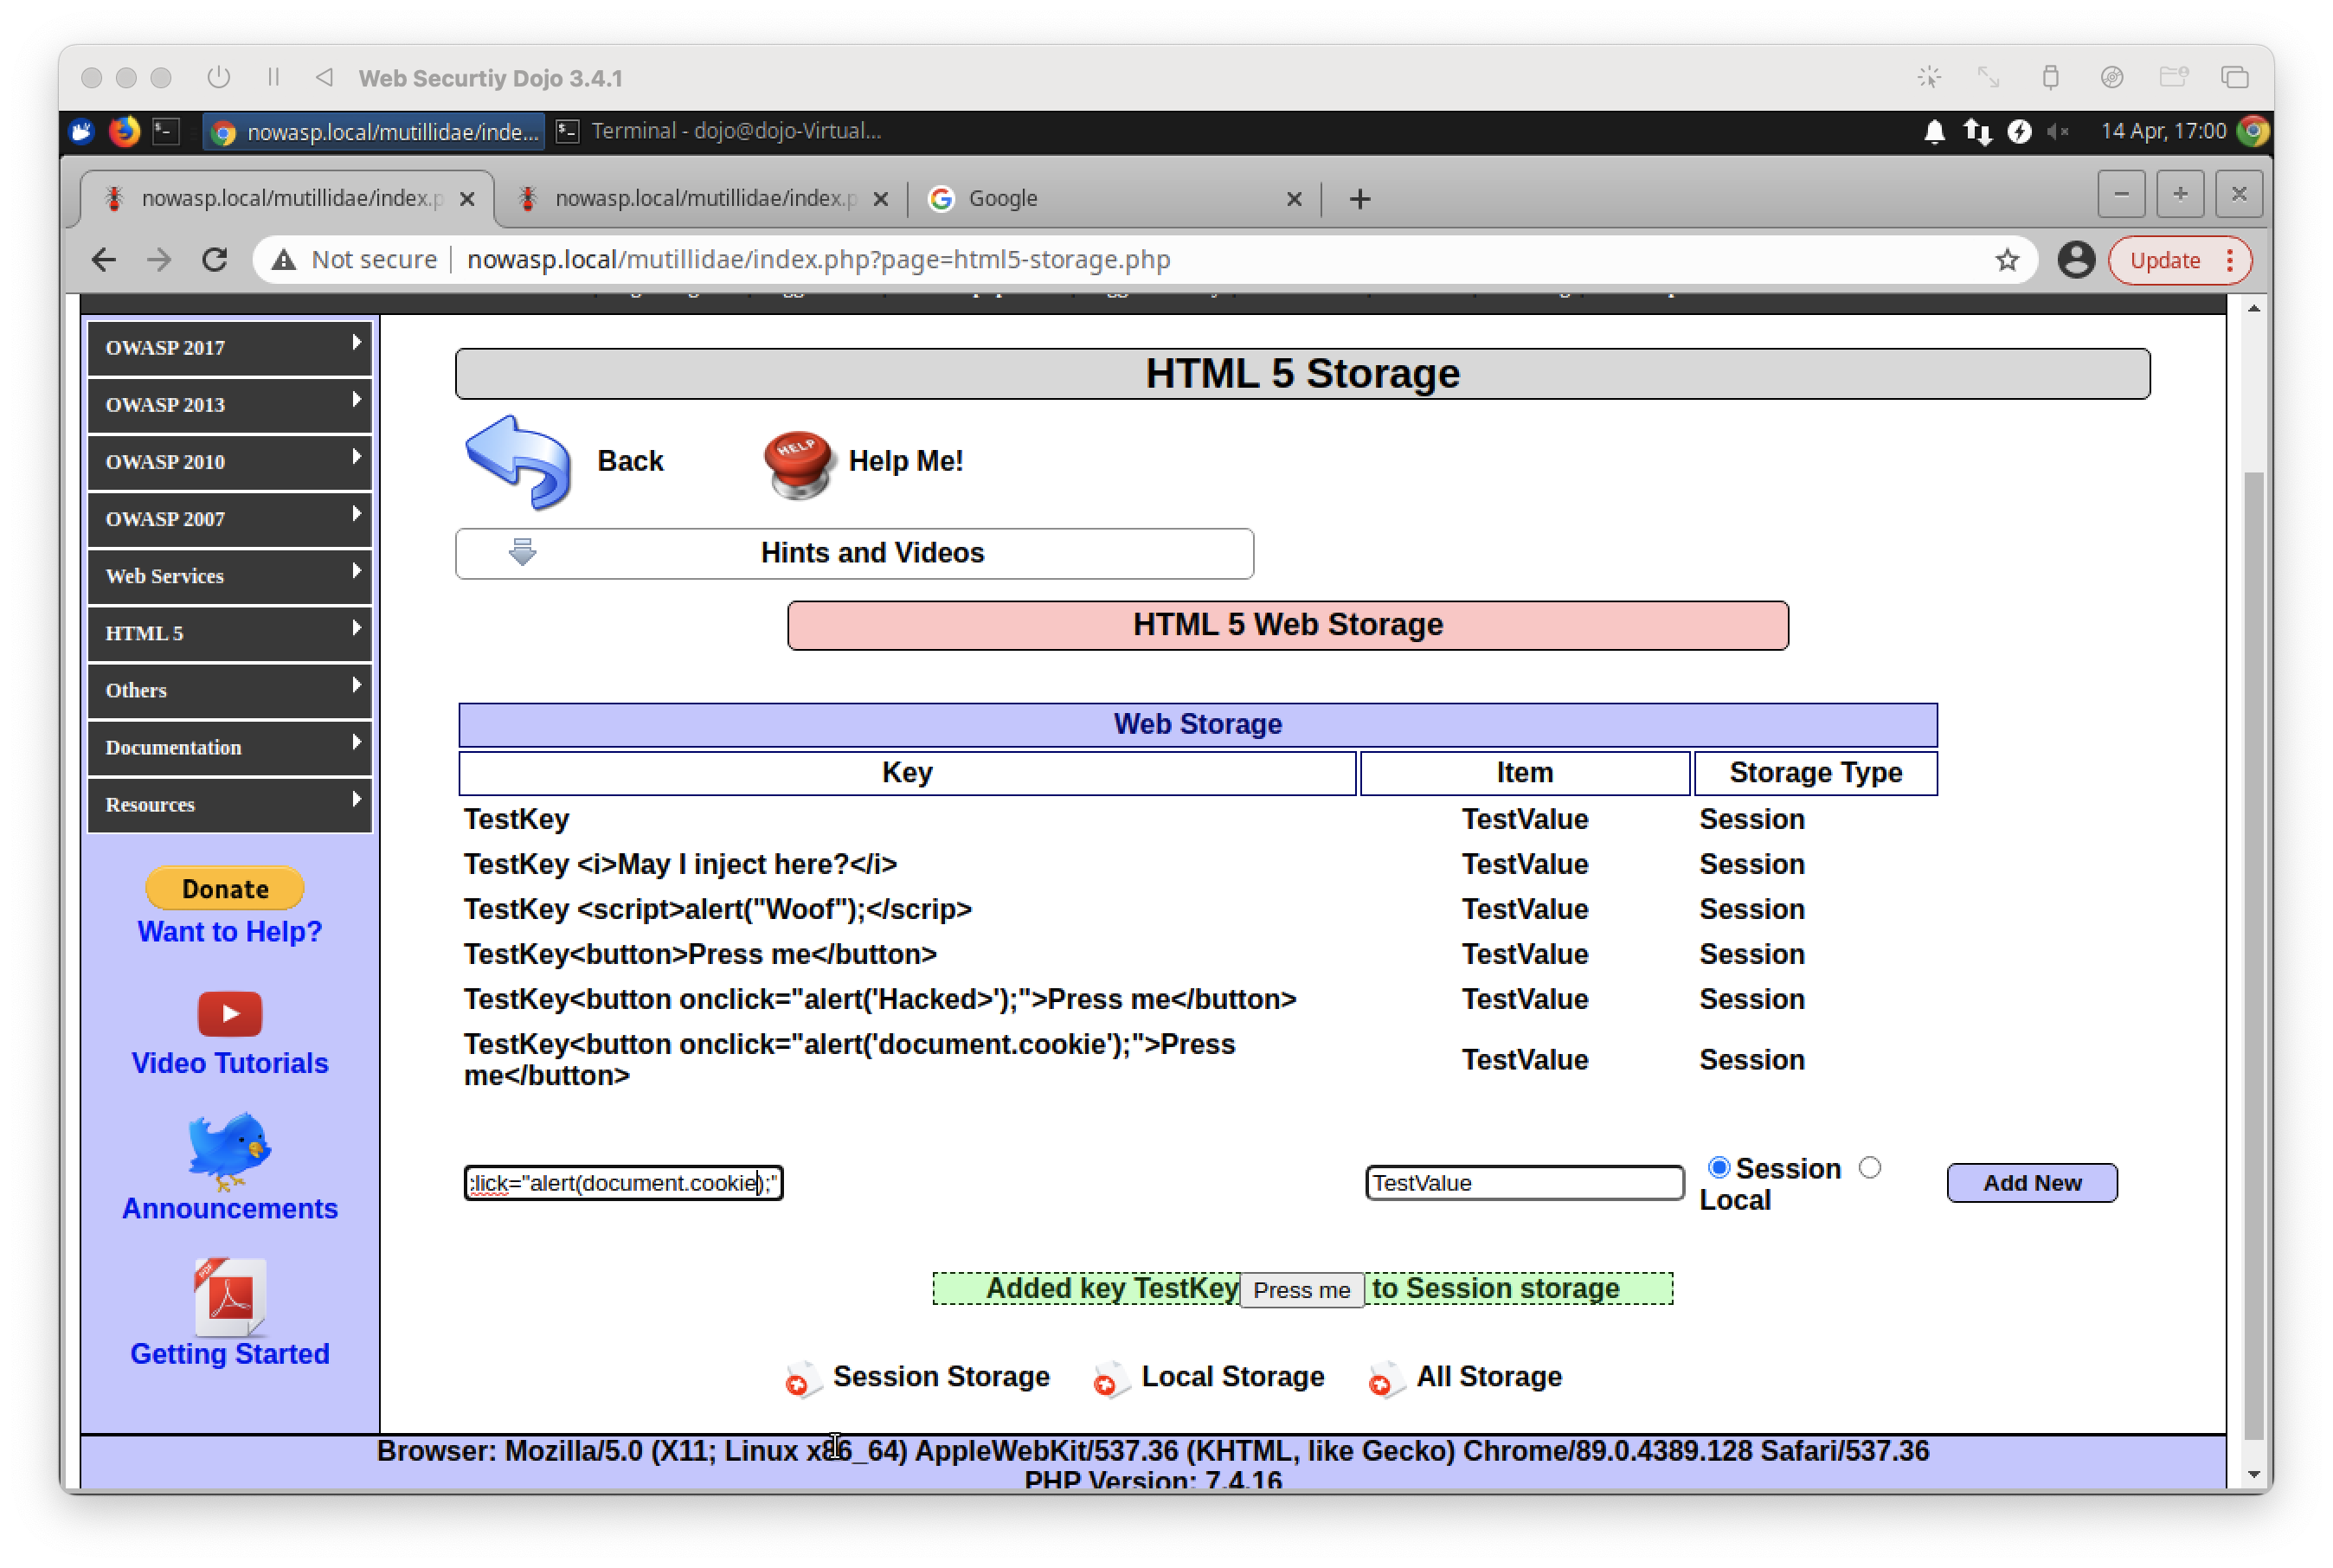
\includegraphics[width=0.8\textwidth]{step_00047}
    \caption{Сделаем это через обычное сообщение}
  \end{figure}

  \begin{figure}[H]
    \centering
    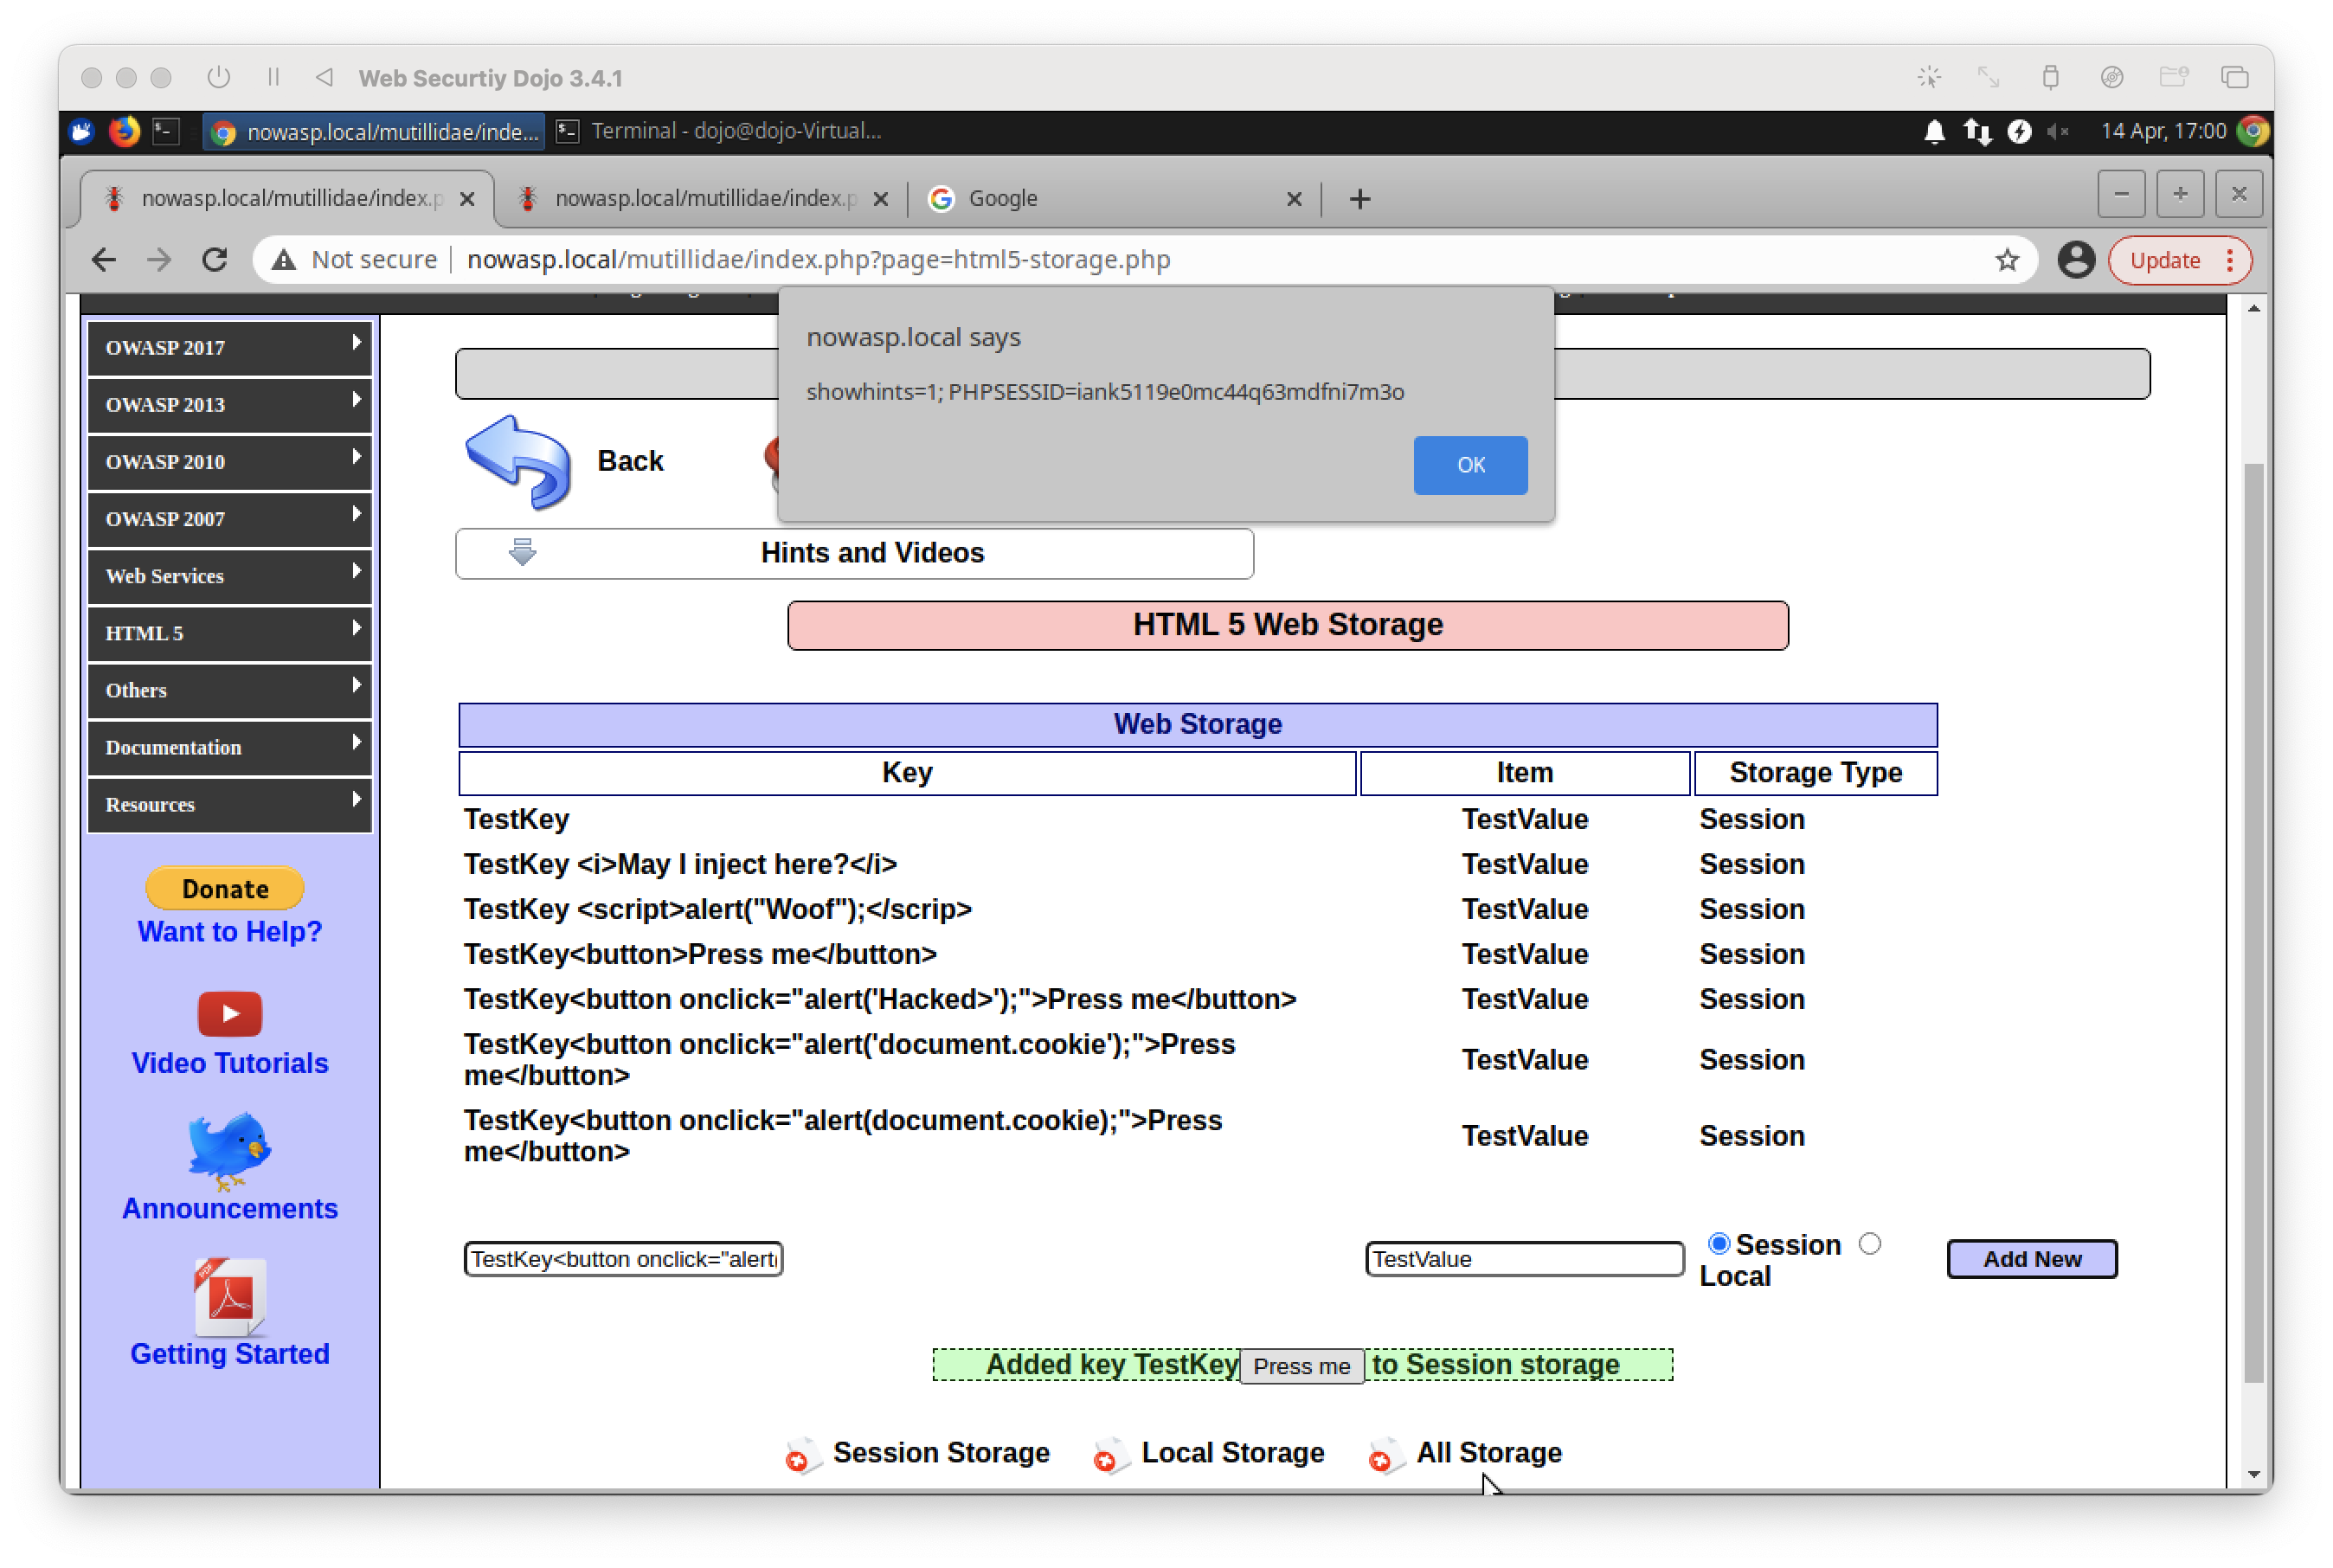
\includegraphics[width=0.8\textwidth]{step_00048}
    \caption{Сессия утекла}
  \end{figure}

  \newpage

  \section{Вывод}

  В ходе данной практической работы были выполнены 3 различные вариа-ции XSS атаки.

\end{document}

